% This file: 			Draft Compiling New Information and Analysis
% Contributors: 		Pietro Biroli, Daniela Del Boca, Linor Kiknadze,
%					Yu Kyung Koh, Sylvi Kuperman, Sidharth Moktan,
%					Chiara Pronzato, Anna Ziff
% Original date: 		10/3/16
% Project: 			Reggio Evaluation

\documentclass[12pt]{article}
\usepackage[top=1in, bottom=1in, left=1in, right=1in]{geometry}
\parindent 22pt

\usepackage{adjustbox}
\usepackage{amsmath}
\usepackage{amssymb}
\usepackage{array}
\usepackage{booktabs}
\usepackage{datetime}
\usepackage{fancyhdr}
\usepackage{float}
\usepackage{graphicx}
\usepackage[colorlinks=true,linkcolor=blue,urlcolor=blue,anchorcolor=blue,citecolor=blue]{hyperref}
\usepackage{lscape}
\usepackage{multirow}
\usepackage{natbib}
\usepackage{setspace}
\usepackage{tabularx}
\usepackage[colorinlistoftodos,linecolor=black]{todonotes}
\usepackage{appendix}
\usepackage{pgffor}
\usepackage{caption} 
\usepackage{threeparttable}
\captionsetup[table]{skip=3pt}

\settimeformat{hhmmsstime}

\newcolumntype{L}[1]{>{\raggedright\arraybackslash}p{#1}}
\newcolumntype{C}[1]{>{\centering\arraybackslash}p{#1}}
\newcolumntype{R}[1]{>{\raggedleft\arraybackslash}p{#1}}

\setcounter{table}{0}
\renewcommand{\thetable}{A\arabic{table}}
\setcounter{figure}{0}
\renewcommand{\thefigure}{A\arabic{figure}}

\externaldocument{reggioEvaluation_main}

\begin{document}

\title{\Large \textbf{Additional Materials}}
\author{\normalsize Reggio Team}
\date{\normalsize Original version: October 3, 2016 \\ Current version: \today}
\maketitle

\textbf{[JJH: Can we present the full set of responses to these questions?][We have most of the responses in Table~\ref{tab:programoperation} through Table~\ref{tab:environ-features} in Appendix~\ref{sec:survey} and discuss the results more in Section~\ref{sec:ece-italy}.]}

\tableofcontents

\doublespacing

\begin{appendices}

\section{Historical Survey}
\label{sec:survey}
The survey below was written to understand the different preschool and infant-toddler programs that were present in Reggio Emilia, Parma, and Padova from the 1950's to present day. It is designed to quantify similarities and differences between the Reggio Approach and other educational programming for young children that were available to the families of each cohort. The survey focuses on administrative features and program operations; pedagogy and curricula; timing of quality improvements; variation within systems and across cities; sources of funding and costs to families; and services for immigrant families.

We administered the survey to current and retired school administrators and educative coordinators from each system in each city. Survey responses were received that allowed us to document the following programs in each decade from 1950: in Reggio Emilia, municipal and state; in Parma, municipal; and in Padova, municipal, state, and religious. Responses were also received from religious systems in Reggio Emilia and in Parma, however, they did not include historical data.

\subsection{Teacher-Child Ratios}
Although in Reggio Emilia, the teacher-child ratio for each classroom has been 2:25 since the 1960s, this number does not reflect the atelierista present at each school site, nor the pedagogista who supervises the educative staff of 4-5 schools. 

In Padova, the municipal preschool system began to consolidate in 1973, expanding from two to five sites by 1976. Teacher-child ratios for Padova's municipal preschools ranged from 1:12 to 1:24 in 1976. There were three state preschools in Padova by 1976; enrollment was relatively lower and teacher-child ratio approximately 1:15. In this same period, teacher-child ratios at religious schools ranged from 1:34-44. 
 
\subsection{Sources of Funding and Costs to Families }
Until the early 2000s, tuition and fees to families enrolling children in religious preschools in all three cities were relatively more expensive than municipal and state programs. After the 2000s, religious schools acknowledged by the state for meeting quality components were eligible to receive state funding. Public funding across the three school systems is not equitably distributed. 

Religious schools in Padova did not receive any form of public funding in the 1970s; families were responsible for 100\% of the costs. In the 1980s and 1990s, the municipality of Padova contributed 20\% and 40\% of program costs to religious schools. In the 2000s, families paid 60\% and the remaining 40\% was shared by the state and municipality of Padova. Municipal schools in Padova are free, families pay only for meals. For state schools, families in Padova also make a voluntary contribution, usually to accommodate expenses associated with field trips.\footnote{This information is further supported by an interview with Dr. Emilia Restiglian of University of Padua.}  
 
Although eligible, the municipality of Reggio Emilia did not receive state funding for its preschool system until the 1990s and 2000s. Ironically, the municipality of Reggio Emilia contributed funds to its state schools each decade since the 1970s. Reggio Emilia also provided training for religious school teachers, beginning in 1994.  

\subsection{Full Survey}

\includepdf[pages=-]{section/CEHD-ECE-Italy_SurveyQuestionnaire-ENGLISH_2016-10-24_sk}

\section{Description of Early Childhood Programs in Italy}
\label{sec:programdes}

\textbf{[Sylvi: Please note that the following program descriptions have been revised from the previous draft to reflect the full set of survey results.]} 

\subsection{State Preschools}

The state regulates and provides preschool education for ages 3-6 years, however, it does not provide infant-toddler programs. State preschools are administered according to legislated policies. Educational practices are guided by Orientamenti which define program standards and general goals for early childhood education. Orientamenti are revised periodically to reflect political ideology and contemporary academic practices. Historically, however, early childhood policies were not consistently enforced throughout Italy, nor were Orientamenti considered binding. 

The cohorts in our sample thus had differential access to state preschools within and across cities; those who enrolled in state programs experienced varying early childhood curricula and administrative practices. The Age 40 cohort had access to 3 or fewer state preschools in each city \citep{Reggio-Admin-data_1966-2006, Reggio-Annual-Journals_1994-2011, Padova-Admin-Data_1964-2011}.\footnote{This sample is too small to distinguish in our evaluation.} In 1969, the first Orientamenti for free state preschools provided only vague guidelines for early childhood education, development and physical care \citep{Corsaro_1996_Early-Edu,Hohnerlein_2015_Development-and-Diffusion}. Children of the age 40 cohort enrolled in state preschools experienced: a) prioritized enrollment for children with disabilities; b) classrooms staffed with 2 fully trained teachers; and, c) male teachers \citep{Hohnerlein_2015_Development-and-Diffusion}. Children of the age 30 cohort who enrolled in state preschools experienced teacher child-ratios of 2:35, mandated in 1980. Both Adult cohorts in state preschools were taught by teachers trained in Catholic institutions, as opposed to secular and academic institutions.

The Adolescent and Child cohorts had access to several improvements in state preschools than did the Adult cohorts. In 1991, revised Orientamenti first emphasized social, affective and cognitive development; Play, collaboration, and mealtime skills were promoted as the key tasks of early childhood \citep{Corsaro_1996_Early-Edu}. In 1997, new mandates required university degrees and supervised experience for state teachers and equivalent pay to teachers in primary schools \citep{Ghedini_2001_Ital-Natl-Policy}. 

In contrast to the Reggio Approach, teaching practices reflect direct instruction as well as play-based learning \citep{CEHD_2016_Historical-Analysis}. Religious teaching is offered, and parents can opt out.\foonote{Alternative educational experiences, however, may not be offered during this time.} Teachers in state preschools work 33 hours per week than their municipal counterparts, who work 36 hours/week. To meet the maximum of 33 hours within an 8 hour school day, one state teacher arrives at 8am, while the second arrives midday and stays until all parents pick up at 4pm. Children in state preschools thus spend more time in a classroom staffed by only 1 teacher than children in municipal schools. Teachers in state preschools further have less weekly time set aside for professional training, documentation, and engagement of parents.

\subsection{Religious Schools}

\textbf{[JJH: I thought we were to use this. Sylvi: Correct, we will ensure the term remains consistent throughout.]}

The Catholic Church offers the majority of religious education and is the oldest of the three early childhood systems, providing for disadvantaged children since the 19th century \citep{OECD_2001_Italy-Country-Note}. All five cohorts in our evaluation had access to religious programming for ages 3-6 years. While infant-toddler religious education was not available for Adults and Adolescents cohorts, spillover from local municipal systems is evident in the availability of transitional religious programming for children aged 24 months for the Child cohorts in Reggio Emilia, Parma, and Padova \citep{Malizia-Cicatelli_2011_BOOK_Catholic-School}. 

Compared to Reggio Emilia and Parma, Padova offers the largest number of religious preschool programs. Compared to the municipal systems in each city, however, teacher-child ratios at Padova's religious schools are much higher. In the 1970s, historical records indicate one teacher for 34-44 preschool-aged children. By the late 1990s, equitable religious programming in each city would require hiring and staffing of teachers at state mandated minimums.

Historically, religious preschools were options only for families that could afford the expense \citep{Hohnerlein_2009_Paradox-Public-Preschools,Ribolzi_2013_Italy}. Prior to 2000, state funding for private schools reflected a 1947 constitutional clause that non-state schools could operate ``without financial burdens on the state.''  \citep{Hohnerlein_2009_Paradox-Public-Preschools}. Accordingly, tuition and fees for religious preschool programs in all three cities were relatively more expensive than municipal and state programs for the oldest four cohorts. Survey results and historical records indicate that religious schools in Padova did not receive any form of public funding in the 1970s; families of the Age 40 cohort who chose religious preschools were responsible for 100\% of the costs. In the 1980s, when the Age 30 cohort was eligible to attend, the municipality of Padova subsidized 20\% of program costs for local religious schools. In the 1990s, when Adolescents were eligible to attend, Padova contributed 40\% of program costs to local religious schools. In the 2000s, when the Child cohort was eligible, families paid 60\%; the remaining 40\% was shared by the state and by Padova \citep{Reggio-Admin-data_1966-2006, Reggio-Annual-Journals_1994-2011, Padova-Admin-Data_1964-2011,CEHD_2016_Historical-Analysis}. 

\subsection{The Municipality of Reggio Emilia}

Reggio Emilia's municipal system currently offers 19 preschool centers. Its infant-toddler system includes 9 full-day centers and 3 part-day centers; infants are eligible to attend from 3 months of age. The municipality further contracts with local private providers to offer a limited number of preschool and infant-toddler slots to resident families according to municipal regulations. While eligible, Reggio Emilia did not receive state funding for its municipal early childhood system until the 1990s and 2000s.\footnote{Ironically, the municipality contributed funds to its local state schools each decade from the 1970s. In 1994, Reggio Approach staff provided training for religious preschool teachers in Reggio Emilia.}
% Maybe for the discussion? Last two sentences above

Survey results indicate that from the 1990s to the present, contracted preschool and infant providers offer programming that vary quite a bit from each other, and vary somewhat from the Reggio Approach. Survey results further indicate the Reggio municipal system predicts its own programs vary a lot from those in Parma's municipal system, and vary a great deal from those in Padova's municipal system \citep{CEHD_2016_Historical-Analysis}. In our evaluation, we do not include former attendees of contracted programs within Reggio Emilia from any of the five cohorts in the evaluation of those who attended Reggio Approach schools. 

\subsection{The Municipality of Parma}

Parma's municipal early childhood system consolidated and expanded around 1975, about a decade after that of Reggio Emilia. Parma's municipal early childhood system is comparatively smaller than Reggio Emilia, currently offering 12 municipal preschools, 8 municipal infant-toddler centers, and 4 ``experimental'' centers for children aged 18 months through 6 years. Distinct from Reggio Emilia, the earliest age of entry into infant programs is later, ranging from 5 to 9 months. 

Like Reggio Emilia, Parma contracts with private and cooperative preschool and infant-toddler providers to meet mandated regulations for provisioning by local demand. Survey results indicate that the programming of contracted providers varies quite a bit from Parma's municipal early childhood approach.\footnote{We do not include former attendees of contracted programs within Parma in the sample of those who attended Parma municipal schools.} Parma predicts that its own municipal system varies a lot from that of Reggio Emilia. The municipality of Parma currently receives state funds for its municipal programs; survey results state funding was first provided in 1980s \citep{CEHD_2016_Historical-Analysis}.

Detailed documentation of Parma's municipal preschools is limited; Conversation with experts familiar with the region suggest that the pedagogical approach of Parma's municipal early childhood system is similar to that of Reggio Emilia.\footnote{Kuperman, Interview with Carolyn Pope Edwards, 2016.} In 2001,\citet{Terzi-Cantarelli_2001_Parma} offer descriptions of Parma's infant-toddler programming that do indeed appear very similar to the Reggio Approach. In contrast to Reggio Emilia, where children are eligible from age 3 months, Parma's infant-toddler programs enroll children beginning at age 5 months. Educative Coordinators perform both administrative and professional development roles similar to Pedagogistas in Reggio Emilia. Assigned to a specific set of infant-toddler centers, Educative Coordinators meet twice each month with all teachers collectively for shared reflection, on-site supervision, and to promote relationships with the families. The city director meets biweekly with Educative Coordinators for overall planning. University professors or administrators from other municipalities provide professional development in the form of continuing education \citep{Terzi-Cantarelli_2001_Parma}. Classrooms are organized by single-age groups (e.g., 5-12 months, 12-24 months, and 24-36 months) or by mixed-age groups (e.g.,12-36 months) \citep{Majorano-etal_2009_CC-in-P}. Mixed-age classes include 18 total children from 13 months to 3 years in a single section, led by two teachers for a 1:9 teacher-child ratio. To accommodate parents, extended hours are available at infant-toddler centers as are three pick-up times: 2 p.m. (short-day), 3:30 p.m. (normal-day), or 5 p.m. (extended-day).

\subsection{The Municipality of Padova}

Padova's municipal preschool system began to consolidate in 1973, expanding from two to five sites by 1976. Padova's municipal preschool system currently offers 10 preschool centers and 17 infant-toddler centers. Padova, distinct from Reggio Emilia and Parma, offers free municipal preschool, and families pay only for meals. Eligible age of entry to infant-toddler programs varies across sites, ranging from 3 to 13 months of age. Like Reggio Emilia and Parma, Padova charges families for infant-toddler programming. 

Reports and survey data suggest that provisioning and quality improvements in Padova's municipal early childhood system was the last of the three cities in our evaluation to evolve. Administrative records from 1976 indicate that teacher-child ratios in Padova's early municipal preschools ranged up to 1:24 \citep{Padova-Admin-Data_1964-2011,CEHD_2016_Historical-Analysis}. In 1989, the region of Veneto reported a total provision of childcare slots for 3.9\% of its infant-toddler population. In contrast, the region of Emilia Romagna reported a provision of infant-toddler childcare for 15.6\% of its population. Professional development for Padova's municipal early childhood staff first began in the mid-1980s, about 20 years after Reggio Emilia and a decade after Parma \citep{Becchi-Ferrari_1990_Pub-Inf-Centres-Italy,CEHD_2016_Historical-Analysis}. In Padova, educative coordinators were actually full-time teachers who were additionally tasked to serve this role on a rotating basis. Not until 2010 did Padova invest in providing pedagogical leaders for the educational staff of its municipal schools. Survey results indicate that Padova first received state funds for its municipal early childhood programs in the 1980s, and additionally received funds from the region of Veneto in the 1990s and 2000s. 

%In Padova, state preschools are also free, however, families are expected to make an additional contribution to accommodate expenses associated with field trips.\citep{CEHD_2016_Historical-Analysis}. In 1976, there were three state preschools in Padova; enrollment was relatively lower compared to religious and municipal programs. In the newly provided state preschools, teacher-child ratios were approximately 1:15.


\section{Additional Information on Outcome and Baseline Data}
\label{sec:data-app}
\subsection{Description of Data}

Table \ref{table:summaryStat_baseline} presents summary statistics for baseline variables by cohort and city. As mentioned above, certain baseline variables are missing for the adult cohorts due to differences in questionnaires administered to adults and children. The table illustrates differences and similarities in parental, caregiver and family characteristics across cities as well as over time. \textbf{[JJH: What is CAPI?][Team: We have fixed the description]}

\begin{landscape}
\singlespace
\setlength{\tabcolsep}{2pt}
\begin{center}
\scriptsize{
\begin{longtable}{L{6cm} c c c p{.5cm} c c c p{.5cm} c c c p{.5cm} c c c p{.5cm} c c c}
\hline\multicolumn{20}{L{24cm}}{\textbf{Note:} Means are reported for each variable by cohort and city. Standard Deviations are reported in italics below each mean estimate. A . denotes that the variable is not defined for a specific cohort.}
\endfoot
\caption{Summary statistics for baseline variables by cohort and city} \label{table:summaryStat_baseline} \\
\hline
& \multicolumn{3}{c}{\textbf{Children}} & & \multicolumn{3}{c}{\textbf{Adolescents}} & & \multicolumn{3}{c}{\textbf{Adults 30}} & & \multicolumn{3}{c}{\textbf{Adults 40}} & & \multicolumn{3}{c}{\textbf{Adults 50}}\\
& \scriptsize{Reggio} & \scriptsize{Parma}& \scriptsize{Padova} & & \scriptsize{Reggio} & \scriptsize{Parma}& \scriptsize{Padova} & & \scriptsize{Reggio} & \scriptsize{Parma}& \scriptsize{Padova} & & \scriptsize{Reggio} & \scriptsize{Parma}& \scriptsize{Padova} & & \scriptsize{Reggio} & \scriptsize{Parma}& \scriptsize{Padova}\\
\hline \\[.2em] \endhead
 \quad Male & 0.54 &      0.56 &      0.52 & &      0.43 &      0.44 &      0.48 & &      0.60 &      0.53 &      0.55 & &      0.54 &      0.49 &      0.48 & &      0.47 &      0.38 &      0.46 \\*
 \quad & $\mathit{     0.50}$ & $\mathit{     0.50}$ & $\mathit{     0.50}$ & & $\mathit{     0.50}$ & $\mathit{     0.50}$ & $\mathit{     0.50}$ & & $\mathit{     0.49}$ & $\mathit{     0.50}$ & $\mathit{     0.50}$ & & $\mathit{     0.50}$ & $\mathit{     0.50}$ & $\mathit{     0.50}$ & & $\mathit{     0.50}$ & $\mathit{     0.49}$ & $\mathit{     0.50}$ \\[.2em]
 \quad Low birthweight & 0.08 &      0.07 &      0.05 & &      0.05 &      0.06 &      0.05 & &         . &         . &         . & &         . &         . &         . & &         . &         . &         . \\*
 \quad & $\mathit{     0.27}$ & $\mathit{     0.25}$ & $\mathit{     0.21}$ & & $\mathit{     0.23}$ & $\mathit{     0.24}$ & $\mathit{     0.21}$ & & $\mathit{        .}$ & $\mathit{        .}$ & $\mathit{        .}$ & & $\mathit{        .}$ & $\mathit{        .}$ & $\mathit{        .}$ & & $\mathit{        .}$ & $\mathit{        .}$ & $\mathit{        .}$ \\[.2em]
 \quad Premature birth & 0.10 &      0.08 &      0.07 & &      0.06 &      0.10 &      0.07 & &         . &         . &         . & &         . &         . &         . & &         . &         . &         . \\*
 \quad & $\mathit{     0.30}$ & $\mathit{     0.26}$ & $\mathit{     0.25}$ & & $\mathit{     0.24}$ & $\mathit{     0.30}$ & $\mathit{     0.25}$ & & $\mathit{        .}$ & $\mathit{        .}$ & $\mathit{        .}$ & & $\mathit{        .}$ & $\mathit{        .}$ & $\mathit{        .}$ & & $\mathit{        .}$ & $\mathit{        .}$ & $\mathit{        .}$ \\[.2em]
 \quad CAPI & 0.55 &      0.43 &      0.47 & &      0.43 &      0.55 &      0.49 & &      0.57 &      0.40 &      0.35 & &      0.63 &      0.34 &      0.35 & &      0.45 &      0.35 &      0.28 \\*
 \quad & $\mathit{     0.50}$ & $\mathit{     0.50}$ & $\mathit{     0.50}$ & & $\mathit{     0.50}$ & $\mathit{     0.50}$ & $\mathit{     0.50}$ & & $\mathit{     0.50}$ & $\mathit{     0.49}$ & $\mathit{     0.48}$ & & $\mathit{     0.48}$ & $\mathit{     0.48}$ & $\mathit{     0.48}$ & & $\mathit{     0.50}$ & $\mathit{     0.48}$ & $\mathit{     0.45}$ \\[.2em]
 \quad Born to teenaged mother & 0.00 &      0.01 &      0.01 & &      0.01 &      0.02 &      0.00 & &      1.00 &      1.00 &      1.00 & &      1.00 &      1.00 &      1.00 & &      1.00 &      1.00 &      1.00 \\*
 \quad & $\mathit{     0.00}$ & $\mathit{     0.08}$ & $\mathit{     0.08}$ & & $\mathit{     0.11}$ & $\mathit{     0.12}$ & $\mathit{     0.00}$ & & $\mathit{     0.00}$ & $\mathit{     0.00}$ & $\mathit{     0.00}$ & & $\mathit{     0.00}$ & $\mathit{     0.00}$ & $\mathit{     0.00}$ & & $\mathit{     0.00}$ & $\mathit{     0.00}$ & $\mathit{     0.00}$ \\[.2em]
 \quad Mom born in province & 0.51 &      0.60 &      0.69 & &      0.68 &      0.68 &      0.78 & &      0.84 &      0.70 &      0.71 & &      0.80 &      0.74 &      0.63 & &      0.78 &      0.80 &      0.76 \\*
 \quad & $\mathit{     0.50}$ & $\mathit{     0.49}$ & $\mathit{     0.46}$ & & $\mathit{     0.47}$ & $\mathit{     0.47}$ & $\mathit{     0.41}$ & & $\mathit{     0.36}$ & $\mathit{     0.46}$ & $\mathit{     0.46}$ & & $\mathit{     0.40}$ & $\mathit{     0.44}$ & $\mathit{     0.48}$ & & $\mathit{     0.42}$ & $\mathit{     0.40}$ & $\mathit{     0.43}$ \\[.2em]
 \quad Mom Max Edu: Low & 0.17 &      0.07 &      0.10 & &      0.16 &      0.11 &      0.14 & &      0.00 &      0.00 &      0.00 & &      0.02 &      0.00 &      0.00 & &      0.01 &      0.04 &      0.01 \\*
 \quad & $\mathit{     0.38}$ & $\mathit{     0.25}$ & $\mathit{     0.30}$ & & $\mathit{     0.36}$ & $\mathit{     0.31}$ & $\mathit{     0.35}$ & & $\mathit{     0.06}$ & $\mathit{     0.00}$ & $\mathit{     0.00}$ & & $\mathit{     0.13}$ & $\mathit{     0.00}$ & $\mathit{     0.06}$ & & $\mathit{     0.10}$ & $\mathit{     0.19}$ & $\mathit{     0.12}$ \\[.2em]
 \quad Mom Max Edu: Middle School & 0.08 &      0.05 &      0.09 & &      0.09 &      0.10 &      0.11 & &      0.03 &      0.07 &      0.10 & &      0.19 &      0.24 &      0.23 & &      0.41 &      0.55 &      0.64 \\*
 \quad & $\mathit{     0.27}$ & $\mathit{     0.23}$ & $\mathit{     0.29}$ & & $\mathit{     0.29}$ & $\mathit{     0.30}$ & $\mathit{     0.31}$ & & $\mathit{     0.18}$ & $\mathit{     0.25}$ & $\mathit{     0.30}$ & & $\mathit{     0.39}$ & $\mathit{     0.43}$ & $\mathit{     0.42}$ & & $\mathit{     0.49}$ & $\mathit{     0.50}$ & $\mathit{     0.48}$ \\[.2em]
 \quad Mom Max Edu: High School & 0.45 &      0.41 &      0.45 & &      0.48 &      0.44 &      0.43 & &      0.42 &      0.30 &      0.35 & &      0.47 &      0.35 &      0.35 & &      0.36 &      0.26 &      0.18 \\*
 \quad & $\mathit{     0.50}$ & $\mathit{     0.49}$ & $\mathit{     0.50}$ & & $\mathit{     0.50}$ & $\mathit{     0.50}$ & $\mathit{     0.50}$ & & $\mathit{     0.49}$ & $\mathit{     0.46}$ & $\mathit{     0.48}$ & & $\mathit{     0.50}$ & $\mathit{     0.48}$ & $\mathit{     0.48}$ & & $\mathit{     0.48}$ & $\mathit{     0.44}$ & $\mathit{     0.39}$ \\[.2em]
 \quad Mom Max Edu: University & 0.28 &      0.46 &      0.36 & &      0.25 &      0.33 &      0.29 & &      0.55 &      0.63 &      0.54 & &      0.31 &      0.41 &      0.41 & &      0.22 &      0.15 &      0.15 \\*
 \quad & $\mathit{     0.45}$ & $\mathit{     0.50}$ & $\mathit{     0.48}$ & & $\mathit{     0.43}$ & $\mathit{     0.47}$ & $\mathit{     0.46}$ & & $\mathit{     0.50}$ & $\mathit{     0.48}$ & $\mathit{     0.50}$ & & $\mathit{     0.46}$ & $\mathit{     0.49}$ & $\mathit{     0.49}$ & & $\mathit{     0.42}$ & $\mathit{     0.35}$ & $\mathit{     0.36}$ \\[.2em]
 \quad Born to teenaged father & 0.00 &      0.00 &      0.01 & &      0.00 &      0.01 &      0.00 & &      1.00 &      1.00 &      1.00 & &      1.00 &      1.00 &      1.00 & &      1.00 &      1.00 &      1.00 \\*
 \quad & $\mathit{     0.00}$ & $\mathit{     0.06}$ & $\mathit{     0.08}$ & & $\mathit{     0.00}$ & $\mathit{     0.09}$ & $\mathit{     0.06}$ & & $\mathit{     0.00}$ & $\mathit{     0.00}$ & $\mathit{     0.00}$ & & $\mathit{     0.00}$ & $\mathit{     0.00}$ & $\mathit{     0.00}$ & & $\mathit{     0.00}$ & $\mathit{     0.00}$ & $\mathit{     0.00}$ \\[.2em]
 \quad Father born in province & 0.52 &      0.59 &      0.64 & &      0.58 &      0.61 &      0.73 & &      0.87 &      0.79 &      0.76 & &      0.78 &      0.85 &      0.73 & &      0.84 &      0.65 &      0.82 \\*
 \quad & $\mathit{     0.50}$ & $\mathit{     0.49}$ & $\mathit{     0.48}$ & & $\mathit{     0.49}$ & $\mathit{     0.49}$ & $\mathit{     0.44}$ & & $\mathit{     0.34}$ & $\mathit{     0.41}$ & $\mathit{     0.43}$ & & $\mathit{     0.42}$ & $\mathit{     0.36}$ & $\mathit{     0.44}$ & & $\mathit{     0.37}$ & $\mathit{     0.48}$ & $\mathit{     0.38}$ \\[.2em]
 \quad Dad Max Edu: Low & 0.23 &      0.12 &      0.09 & &      0.19 &      0.16 &      0.14 & &         . &         . &         . & &      0.02 &      0.00 &      0.00 & &      0.01 &      0.04 &      0.02 \\*
 \quad & $\mathit{     0.42}$ & $\mathit{     0.33}$ & $\mathit{     0.29}$ & & $\mathit{     0.40}$ & $\mathit{     0.37}$ & $\mathit{     0.35}$ & & $\mathit{        .}$ & $\mathit{        .}$ & $\mathit{        .}$ & & $\mathit{     0.14}$ & $\mathit{     0.06}$ & $\mathit{     0.06}$ & & $\mathit{     0.07}$ & $\mathit{     0.19}$ & $\mathit{     0.14}$ \\[.2em]
 \quad Dad Max Edu: Middle School & 0.08 &      0.10 &      0.09 & &      0.09 &      0.07 &      0.10 & &      0.03 &      0.08 &      0.10 & &      0.19 &      0.22 &      0.14 & &      0.35 &      0.55 &      0.52 \\*
 \quad & $\mathit{     0.27}$ & $\mathit{     0.30}$ & $\mathit{     0.28}$ & & $\mathit{     0.28}$ & $\mathit{     0.26}$ & $\mathit{     0.30}$ & & $\mathit{     0.17}$ & $\mathit{     0.27}$ & $\mathit{     0.30}$ & & $\mathit{     0.39}$ & $\mathit{     0.41}$ & $\mathit{     0.35}$ & & $\mathit{     0.48}$ & $\mathit{     0.50}$ & $\mathit{     0.50}$ \\[.2em]
 \quad Dad Max Edu: High School & 0.35 &      0.36 &      0.42 & &      0.40 &      0.36 &      0.39 & &      0.37 &      0.32 &      0.32 & &      0.45 &      0.33 &      0.27 & &      0.36 &      0.19 &      0.17 \\*
 \quad & $\mathit{     0.48}$ & $\mathit{     0.48}$ & $\mathit{     0.49}$ & & $\mathit{     0.49}$ & $\mathit{     0.48}$ & $\mathit{     0.49}$ & & $\mathit{     0.48}$ & $\mathit{     0.47}$ & $\mathit{     0.47}$ & & $\mathit{     0.50}$ & $\mathit{     0.47}$ & $\mathit{     0.44}$ & & $\mathit{     0.48}$ & $\mathit{     0.40}$ & $\mathit{     0.38}$ \\[.2em]
 \quad Dad Max Edu: University & 0.24 &      0.35 &      0.30 & &      0.19 &      0.26 &      0.28 & &      0.60 &      0.60 &      0.57 & &      0.33 &      0.45 &      0.58 & &      0.27 &      0.20 &      0.27 \\*
 \quad & $\mathit{     0.43}$ & $\mathit{     0.48}$ & $\mathit{     0.46}$ & & $\mathit{     0.39}$ & $\mathit{     0.44}$ & $\mathit{     0.45}$ & & $\mathit{     0.49}$ & $\mathit{     0.49}$ & $\mathit{     0.50}$ & & $\mathit{     0.47}$ & $\mathit{     0.50}$ & $\mathit{     0.49}$ & & $\mathit{     0.45}$ & $\mathit{     0.40}$ & $\mathit{     0.45}$ \\[.2em]
 \quad Has 1 sibling & 0.52 &      0.46 &      0.50 & &      0.52 &      0.46 &      0.55 & &      0.36 &      0.33 &      0.45 & &      0.36 &      0.38 &      0.35 & &      0.28 &      0.26 &      0.39 \\*
 \quad & $\mathit{     0.50}$ & $\mathit{     0.50}$ & $\mathit{     0.50}$ & & $\mathit{     0.50}$ & $\mathit{     0.50}$ & $\mathit{     0.50}$ & & $\mathit{     0.48}$ & $\mathit{     0.47}$ & $\mathit{     0.50}$ & & $\mathit{     0.48}$ & $\mathit{     0.49}$ & $\mathit{     0.48}$ & & $\mathit{     0.45}$ & $\mathit{     0.44}$ & $\mathit{     0.49}$ \\[.2em]
 \quad Has 2 siblings & 0.14 &      0.21 &      0.17 & &      0.18 &      0.20 &      0.15 & &      0.24 &      0.33 &      0.25 & &      0.27 &      0.33 &      0.35 & &      0.30 &      0.27 &      0.22 \\*
 \quad & $\mathit{     0.35}$ & $\mathit{     0.41}$ & $\mathit{     0.37}$ & & $\mathit{     0.38}$ & $\mathit{     0.40}$ & $\mathit{     0.36}$ & & $\mathit{     0.43}$ & $\mathit{     0.47}$ & $\mathit{     0.43}$ & & $\mathit{     0.44}$ & $\mathit{     0.47}$ & $\mathit{     0.48}$ & & $\mathit{     0.46}$ & $\mathit{     0.45}$ & $\mathit{     0.42}$ \\[.2em]
 \quad Has more than 2 siblings & 0.06 &      0.04 &      0.05 & &      0.09 &      0.06 &      0.02 & &      0.13 &      0.20 &      0.17 & &      0.20 &      0.19 &      0.26 & &      0.34 &      0.39 &      0.35 \\*
 \quad & $\mathit{     0.23}$ & $\mathit{     0.19}$ & $\mathit{     0.21}$ & & $\mathit{     0.29}$ & $\mathit{     0.24}$ & $\mathit{     0.16}$ & & $\mathit{     0.33}$ & $\mathit{     0.40}$ & $\mathit{     0.37}$ & & $\mathit{     0.40}$ & $\mathit{     0.39}$ & $\mathit{     0.44}$ & & $\mathit{     0.48}$ & $\mathit{     0.49}$ & $\mathit{     0.48}$ \\[.2em]
 \quad Caregiver was Catholic & 0.77 &      0.83 &      0.79 & &      0.75 &      0.86 &      0.73 & &         . &         . &         . & &         . &         . &         . & &         . &         . &         . \\*
 \quad & $\mathit{     0.42}$ & $\mathit{     0.37}$ & $\mathit{     0.41}$ & & $\mathit{     0.43}$ & $\mathit{     0.35}$ & $\mathit{     0.44}$ & & $\mathit{        .}$ & $\mathit{        .}$ & $\mathit{        .}$ & & $\mathit{        .}$ & $\mathit{        .}$ & $\mathit{        .}$ & & $\mathit{        .}$ & $\mathit{        .}$ & $\mathit{        .}$ \\[.2em]
 \quad Caregiver was faithful and Catholic & 0.47 &      0.52 &      0.51 & &      0.45 &      0.54 &      0.45 & &         . &         . &         . & &         . &         . &         . & &         . &         . &         . \\*
 \quad & $\mathit{     0.50}$ & $\mathit{     0.50}$ & $\mathit{     0.50}$ & & $\mathit{     0.50}$ & $\mathit{     0.50}$ & $\mathit{     0.50}$ & & $\mathit{        .}$ & $\mathit{        .}$ & $\mathit{        .}$ & & $\mathit{        .}$ & $\mathit{        .}$ & $\mathit{        .}$ & & $\mathit{        .}$ & $\mathit{        .}$ & $\mathit{        .}$ \\[.2em]
 \quad Caregiver owned house & 0.58 &      0.71 &      0.66 & &      0.84 &      0.81 &      0.77 & &         . &         . &         . & &         . &         . &         . & &         . &         . &         . \\*
 \quad & $\mathit{     0.49}$ & $\mathit{     0.46}$ & $\mathit{     0.48}$ & & $\mathit{     0.37}$ & $\mathit{     0.39}$ & $\mathit{     0.42}$ & & $\mathit{        .}$ & $\mathit{        .}$ & $\mathit{        .}$ & & $\mathit{        .}$ & $\mathit{        .}$ & $\mathit{        .}$ & & $\mathit{        .}$ & $\mathit{        .}$ & $\mathit{        .}$ \\[.2em]
 \quad Caregiver was a migrant & 0.07 &      0.02 &      0.02 & &      0.01 &      0.02 &      0.00 & &         . &         . &         . & &         . &         . &         . & &         . &         . &         . \\*
 \quad & $\mathit{     0.26}$ & $\mathit{     0.14}$ & $\mathit{     0.15}$ & & $\mathit{     0.11}$ & $\mathit{     0.12}$ & $\mathit{     0.00}$ & & $\mathit{        .}$ & $\mathit{        .}$ & $\mathit{        .}$ & & $\mathit{        .}$ & $\mathit{        .}$ & $\mathit{        .}$ & & $\mathit{        .}$ & $\mathit{        .}$ & $\mathit{        .}$ \\[.2em]
 \quad Caregiver Income: 5,000 euros or less & 0.01 &      0.02 &      0.03 & &      0.00 &      0.02 &      0.04 & &         . &         . &         . & &         . &         . &         . & &         . &         . &         . \\*
 \quad & $\mathit{     0.11}$ & $\mathit{     0.15}$ & $\mathit{     0.18}$ & & $\mathit{     0.06}$ & $\mathit{     0.15}$ & $\mathit{     0.19}$ & & $\mathit{        .}$ & $\mathit{        .}$ & $\mathit{        .}$ & & $\mathit{        .}$ & $\mathit{        .}$ & $\mathit{        .}$ & & $\mathit{        .}$ & $\mathit{        .}$ & $\mathit{        .}$ \\[.2em]
 \quad Caregiver Income: 5,001-10,000 euros & 0.01 &      0.02 &      0.01 & &      0.01 &      0.01 &      0.01 & &         . &         . &         . & &         . &         . &         . & &         . &         . &         . \\*
 \quad & $\mathit{     0.11}$ & $\mathit{     0.13}$ & $\mathit{     0.12}$ & & $\mathit{     0.10}$ & $\mathit{     0.09}$ & $\mathit{     0.08}$ & & $\mathit{        .}$ & $\mathit{        .}$ & $\mathit{        .}$ & & $\mathit{        .}$ & $\mathit{        .}$ & $\mathit{        .}$ & & $\mathit{        .}$ & $\mathit{        .}$ & $\mathit{        .}$ \\[.2em]
 \quad Caregiver Income: 10,001-25,000 euros & 0.17 &      0.19 &      0.15 & &      0.18 &      0.18 &      0.10 & &         . &         . &         . & &         . &         . &         . & &         . &         . &         . \\*
 \quad & $\mathit{     0.38}$ & $\mathit{     0.39}$ & $\mathit{     0.36}$ & & $\mathit{     0.39}$ & $\mathit{     0.38}$ & $\mathit{     0.30}$ & & $\mathit{        .}$ & $\mathit{        .}$ & $\mathit{        .}$ & & $\mathit{        .}$ & $\mathit{        .}$ & $\mathit{        .}$ & & $\mathit{        .}$ & $\mathit{        .}$ & $\mathit{        .}$ \\[.2em]
 \quad Caregiver Income: 25,001-50,000 euros & 0.32 &      0.41 &      0.32 & &      0.32 &      0.29 &      0.24 & &         . &         . &         . & &         . &         . &         . & &         . &         . &         . \\*
 \quad & $\mathit{     0.47}$ & $\mathit{     0.49}$ & $\mathit{     0.47}$ & & $\mathit{     0.47}$ & $\mathit{     0.46}$ & $\mathit{     0.43}$ & & $\mathit{        .}$ & $\mathit{        .}$ & $\mathit{        .}$ & & $\mathit{        .}$ & $\mathit{        .}$ & $\mathit{        .}$ & & $\mathit{        .}$ & $\mathit{        .}$ & $\mathit{        .}$ \\[.2em]
 \quad Caregiver Income: 50,001-100,000 euros & 0.19 &      0.19 &      0.13 & &      0.24 &      0.24 &      0.11 & &         . &         . &         . & &         . &         . &         . & &         . &         . &         . \\*
 \quad & $\mathit{     0.40}$ & $\mathit{     0.39}$ & $\mathit{     0.34}$ & & $\mathit{     0.43}$ & $\mathit{     0.43}$ & $\mathit{     0.31}$ & & $\mathit{        .}$ & $\mathit{        .}$ & $\mathit{        .}$ & & $\mathit{        .}$ & $\mathit{        .}$ & $\mathit{        .}$ & & $\mathit{        .}$ & $\mathit{        .}$ & $\mathit{        .}$ \\[.2em]
 \quad Caregiver Income: 100,001-250,000 euros & 0.02 &      0.02 &      0.03 & &      0.04 &      0.03 &      0.02 & &         . &         . &         . & &         . &         . &         . & &         . &         . &         . \\*
 \quad & $\mathit{     0.15}$ & $\mathit{     0.14}$ & $\mathit{     0.17}$ & & $\mathit{     0.20}$ & $\mathit{     0.17}$ & $\mathit{     0.16}$ & & $\mathit{        .}$ & $\mathit{        .}$ & $\mathit{        .}$ & & $\mathit{        .}$ & $\mathit{        .}$ & $\mathit{        .}$ & & $\mathit{        .}$ & $\mathit{        .}$ & $\mathit{        .}$ \\[.2em]
 \quad Caregiver Income: > 250,000 euros & . &         . &         . & &      0.00 &      0.00 &      0.00 & &         . &         . &         . & &         . &         . &         . & &         . &         . &         . \\*
 \quad & $\mathit{        .}$ & $\mathit{        .}$ & $\mathit{        .}$ & & $\mathit{     0.06}$ & $\mathit{     0.00}$ & $\mathit{     0.00}$ & & $\mathit{        .}$ & $\mathit{        .}$ & $\mathit{        .}$ & & $\mathit{        .}$ & $\mathit{        .}$ & $\mathit{        .}$ & & $\mathit{        .}$ & $\mathit{        .}$ & $\mathit{        .}$ \\[.2em]
 \quad Caregiver was religious & 0.85 &      0.87 &      0.80 & &      0.77 &      0.87 &      0.74 & &      0.50 &      0.73 &      0.72 & &      0.50 &      0.75 &      0.75 & &      0.64 &      0.71 &      0.77 \\*
 \quad & $\mathit{     0.36}$ & $\mathit{     0.34}$ & $\mathit{     0.40}$ & & $\mathit{     0.42}$ & $\mathit{     0.34}$ & $\mathit{     0.44}$ & & $\mathit{     0.50}$ & $\mathit{     0.45}$ & $\mathit{     0.45}$ & & $\mathit{     0.50}$ & $\mathit{     0.43}$ & $\mathit{     0.44}$ & & $\mathit{     0.48}$ & $\mathit{     0.46}$ & $\mathit{     0.42}$ \\[.2em]
 ~\\[-.5em]
\hline
\end{longtable}
}
\end{center}

\end{landscape}

\subsection{Characteristics of Reggio Emilia, Parma, and Padova}
\label{app:characteristics-cities}

Table~\ref{table:data-sources} lists the sources of the myriad of historical records that we investigated. Tables~\ref{table:demo-employ} and~\ref{table:demo-other} describe the cities along demographic characteristics based on those records. Reggio Emilia and Parma, in addition to being geographically close are socially and economically similar.

\begin{table}[H]
\centering
\footnotesize
	\caption{Summary of Data Sources} \label{table:data-sources}
	\begin{tabular}{lll}
\toprule
\multicolumn{1}{c}{Type}	&	\multicolumn{1}{c}{Variables}	&	\multicolumn{1}{c}{Sources}	\\
\midrule
			&	Population & \\
			& 	Age distribution & \\
			&	Aging index & \\
Census Data	&	Marital status & \citet{Istat_2014_Atlante-Statistico} \\
			& 	Educational attainment & \\
			& 	Economic activity & \\
			& 	Employment by industry & \\
			& 	Homeownership	&	\\
\midrule
						&	Population 		&	 \\
						&	Age distribution 	&	\citet{Reggio-Emilia-Admin-Data_1966-2010}, \\
						&	Birth rates 		& 	\citet{Padova-Admin-Data_1964-2010}, 	\\
	Demographic Statistics	&	Mortality rates 		&	\citet{Statistica-Regionae_2016_Veneto}, \\
						&	Internal migration 	&  	\citet{Emilia-Romagna_2016_Population},\\
						&	Foreign migration 	&	\citet{Statistica-Regionae_2016_Veneto}, \\
						& 	Married in religious ceremonies	& 	and \citet{Istat_2016_Geo-Demo} \\
\midrule
						&	School-level preschool enrollment	 &	Comune di Reggio Emilia, \\
	Early Education Statistics	& 	School-level infant-toddler enrollment & 	\citet{Padova-Admin-Data_1964-2010},  \\
						& 	Child-teacher ratios				&	and \citet{Reggio-Emilia-Admin-Data_1966-2010} \\
\midrule
Election Data				&	\% of Votes to PCI and DC parties 	&	\citet{Archivo-Storico_2016} \\
\bottomrule
\end{tabular}


\end{table}


\begin{landscape}
\begin{table}[ht!]
\begin{center}
\scriptsize{
	\caption{Proportion of Individuals in Different Employment and Industry Categories} \label{table:demo-employ}
	
\begin{tabular}{L{6.5cm} *{3}{*{5}{c} c}}
\hline \\[-7pt]
& \multicolumn{5}{c}{\textbf{Reggio Emilia}} & & \multicolumn{5}{c}{\textbf{Parma}} & & \multicolumn{5}{c}{\textbf{Padova}} \\[3pt]
& \textbf{1971} & \textbf{1981} & \textbf{1991} & \textbf{2001} & \textbf{2011} & & \textbf{1971} & \textbf{1981} & \textbf{1991} & \textbf{2001} & \textbf{2011} & & \textbf{1971} & \textbf{1981} & \textbf{1991} & \textbf{2001} & \textbf{2011} \\[3pt]
\hline \\
\textbf{Employment}\\
\quad Employed (B) & 0.48 & 0.51 & 0.49 & 0.53 & 0.53 & & 0.47 & 0.49 & 0.49 & 0.50 & 0.53 & & 0.45 & 0.46 & 0.45 & 0.47 & 0.49 & \\ 
\quad Employed (F) & 0.28 & 0.37 & 0.38 & 0.43 & 0.46 & & 0.26 & 0.34 & 0.37 & 0.41 & 0.46 & & 0.24 & 0.30 & 0.32 & 0.37 & 0.42 & \\ 
\quad Employed (M) & 0.70 & 0.66 & 0.61 & 0.63 & 0.62 & & 0.70 & 0.66 & 0.62 & 0.60 & 0.60 & & 0.69 & 0.64 & 0.60 & 0.59 & 0.57 & \\[5pt] 
\quad Unemployed (B) & 0.01 & 0.01 & 0.02 & 0.02 & 0.06 & & 0.02 & 0.02 & 0.01 & 0.02 & 0.03 & & 0.02 & 0.01 & 0.02 & 0.03 & 0.04 & \\ 
\quad Unemployed (F) & 0.01 & 0.01 & 0.02 & 0.03 & 0.06 & & 0.01 & 0.02 & 0.01 & 0.02 & 0.03 & & 0.01 & 0.01 & 0.02 & 0.03 & 0.04 & \\ 
\quad Unemployed (M) & 0.02 & 0.01 & 0.02 & 0.02 & 0.05 & & 0.02 & 0.01 & 0.01 & 0.02 & 0.03 & & 0.02 & 0.02 & 0.03 & 0.03 & 0.04 & \\[5pt] 
\quad Homemaker (B) & 0.26 & 0.17 & 0.13 & 0.11 & 0.06 & & 0.28 & 0.20 & 0.16 & 0.12 & 0.07 & & 0.32 & 0.25 & 0.21 & 0.16 & 0.09 & \\ 
\quad Homemaker (F) & 0.50 & 0.33 & 0.25 & 0.20 & 0.11 & & 0.53 & 0.37 & 0.30 & 0.22 & 0.12 & & 0.59 & 0.47 & 0.38 & 0.30 & 0.16 & \\ 
\quad Homemaker (M) & 0.00 & 0.00 & 0.00 & 0.00 & 0.00 & & 0.00 & 0.00 & 0.00 & 0.00 & 0.00 & & 0.00 & 0.00 & 0.00 & 0.00 & 0.01 & \\[5pt] 
\quad Pensioner (B) & 0.15 & 0.21 & 0.23 & 0.24 & 0.25 & & 0.15 & 0.19 & 0.21 & 0.24 & 0.27 & & 0.11 & 0.13 & 0.16 & 0.21 & 0.26 & \\ 
\quad Pensioner (F) & 0.13 & 0.20 & 0.22 & 0.23 & 0.27 & & 0.13 & 0.17 & 0.19 & 0.22 & 0.28 & & 0.07 & 0.09 & 0.12 & 0.18 & 0.27 & \\ 
\quad Pensioner (M) & 0.17 & 0.22 & 0.24 & 0.25 & 0.23 & & 0.18 & 0.21 & 0.23 & 0.26 & 0.25 & & 0.15 & 0.17 & 0.20 & 0.26 & 0.25 & \\[5pt] 
\quad Student (B) & 0.07 & 0.07 & 0.08 & 0.06 & 0.06 & & 0.07 & 0.08 & 0.09 & 0.07 & 0.07 & & 0.09 & 0.11 & 0.11 & 0.08 & 0.08 & \\ 
\quad Student (F) & 0.06 & 0.07 & 0.08 & 0.05 & 0.06 & & 0.06 & 0.08 & 0.08 & 0.06 & 0.06 & & 0.07 & 0.10 & 0.10 & 0.07 & 0.07 & \\ 
\quad Student (M) & 0.08 & 0.08 & 0.08 & 0.06 & 0.07 & & 0.08 & 0.09 & 0.09 & 0.07 & 0.07 & & 0.11 & 0.13 & 0.12 & 0.08 & 0.08 & \\[5pt] 
\quad Other (B) & 0.03 & 0.03 & 0.05 & 0.05 & 0.04 & & 0.02 & 0.02 & 0.04 & 0.05 & 0.04 & & 0.02 & 0.03 & 0.05 & 0.05 & 0.05 & \\ 
\quad Other (F) & 0.03 & 0.02 & 0.05 & 0.05 & 0.04 & & 0.02 & 0.02 & 0.04 & 0.05 & 0.04 & & 0.02 & 0.02 & 0.05 & 0.05 & 0.04 & \\ 
\quad Other (M) & 0.04 & 0.03 & 0.04 & 0.04 & 0.04 & & 0.02 & 0.03 & 0.04 & 0.05 & 0.04 & & 0.03 & 0.04 & 0.05 & 0.05 & 0.05 & \\[5pt] 
\textbf{Industry}\\
\quad Agriculture, Forestry And Fishing (B) &   . & 0.08 & 0.04 & 0.04 & 0.04 & &   . & 0.05 & 0.02 & 0.02 & 0.03 & &   . & 0.01 & 0.01 & 0.01 & 0.01 & \\ 
\quad Agriculture, Forestry And Fishing (F) &   . & 0.06 & 0.03 & 0.03 & 0.02 & &   . & 0.04 & 0.01 & 0.02 & 0.02 & &   . & 0.01 & 0.01 & 0.01 & 0.01 & \\ 
\quad Agriculture, Forestry And Fishing (M) &   . & 0.10 & 0.05 & 0.04 & 0.05 & &   . & 0.05 & 0.03 & 0.03 & 0.04 & &   . & 0.02 & 0.01 & 0.01 & 0.02 & \\[5pt] 
\quad Finance, Professional, Scientific, Admin (B) &   . & 0.07 & 0.11 & 0.11 & 0.14 & &   . & 0.08 & 0.13 & 0.14 & 0.17 & &   . & 0.09 & 0.15 & 0.17 & 0.19 & \\ 
\quad Finance, Professional, Scientific, Admin (F) &   . & 0.06 & 0.12 & 0.12 & 0.15 & &   . & 0.07 & 0.15 & 0.14 & 0.18 & &   . & 0.08 & 0.15 & 0.17 & 0.19 & \\ 
\quad Finance, Professional, Scientific, Admin (M) &   . & 0.07 & 0.10 & 0.11 & 0.13 & &   . & 0.08 & 0.12 & 0.13 & 0.16 & &   . & 0.09 & 0.15 & 0.17 & 0.20 & \\[5pt] 
\quad Trade, Hotels And Restaurants  (B) &   . & 0.19 & 0.20 & 0.19 & 0.18 & &   . & 0.20 & 0.19 & 0.18 & 0.17 & &   . & 0.26 & 0.23 & 0.20 & 0.16 & \\ 
\quad Trade, Hotels And Restaurants  (F) &   . & 0.20 & 0.21 & 0.21 & 0.20 & &   . & 0.21 & 0.21 & 0.20 & 0.18 & &   . & 0.24 & 0.21 & 0.19 & 0.16 & \\ 
\quad Trade, Hotels And Restaurants  (M) &   . & 0.18 & 0.19 & 0.18 & 0.16 & &   . & 0.19 & 0.18 & 0.17 & 0.15 & &   . & 0.26 & 0.23 & 0.20 & 0.17 & \\[5pt] 
\quad Transport, Storage, Info, Communication  (B) &   . & 0.05 & 0.04 & 0.04 & 0.06 & &   . & 0.05 & 0.05 & 0.04 & 0.06 & &   . & 0.06 & 0.05 & 0.05 & 0.07 & \\ 
\quad Transport, Storage, Info, Communication  (F) &   . & 0.02 & 0.03 & 0.02 & 0.03 & &   . & 0.02 & 0.03 & 0.02 & 0.04 & &   . & 0.03 & 0.03 & 0.03 & 0.04 & \\ 
\quad Transport, Storage, Info, Communication  (M) &   . & 0.06 & 0.05 & 0.05 & 0.07 & &   . & 0.07 & 0.06 & 0.05 & 0.08 & &   . & 0.08 & 0.07 & 0.06 & 0.09 & \\[5pt] 
\quad Other Activities  (B) &   . & 0.24 & 0.23 & 0.25 & 0.28 & &   . & 0.25 & 0.25 & 0.28 & 0.31 & &   . & 0.32 & 0.32 & 0.35 & 0.37 & \\ 
\quad Other Activities  (F) &   . & 0.36 & 0.34 & 0.38 & 0.43 & &   . & 0.39 & 0.36 & 0.41 & 0.44 & &   . & 0.47 & 0.44 & 0.47 & 0.51 & \\ 
\quad Other Activities  (M) &   . & 0.16 & 0.16 & 0.15 & 0.15 & &   . & 0.17 & 0.18 & 0.19 & 0.20 & &   . & 0.24 & 0.25 & 0.27 & 0.25 & \\[5pt] 
\hline \\[-7pt]
\multicolumn{19}{L{24cm}}{\textbf{Note:} This table presents the percentage of individuals in different employment and industry categories within each city during each of the 5 listed years. Percentages are reported for females (F), males (M), and both genders (B) combined. The percentages are calculated using the total number of individuals above age 15 for the denominator. Data were collected from ISTAT and regional agencies.}
\end{tabular}

}
\end{center}
\end{table}
\end{landscape}

\begin{landscape}
\begin{table}[ht!]
\begin{center}
\scriptsize{
	\caption{Proportion of Individuals in Different Education, Rental, and Marital Categories} \label{table:demo-other}
	
\begin{tabular}{L{5cm} *{3}{*{5}{c} c}}
\hline \\[-7pt]
& \multicolumn{5}{c}{\textbf{Reggio}} & & \multicolumn{5}{c}{\textbf{Parma}} & & \multicolumn{5}{c}{\textbf{Padova}} \\[3pt]
& \textbf{1971} & \textbf{1981} & \textbf{1991} & \textbf{2001} & \textbf{2011} & & \textbf{1971} & \textbf{1981} & \textbf{1991} & \textbf{2001} & \textbf{2011} & & \textbf{1971} & \textbf{1981} & \textbf{1991} & \textbf{2001} & \textbf{2011} \\[3pt]
\hline \\
~\\[-4pt]
\textbf{Education}\\
\quad $<$ Primary (B) & 0.27 & 0.15 & 0.10 & 0.08 & 0.07 & & 0.28 & 0.14 & 0.09 & 0.07 & 0.06 & & 0.23 & 0.13 & 0.08 & 0.06 & 0.06 & \\ 
\quad $<$ Primary (F) & 0.31 & 0.17 & 0.11 & 0.09 & 0.08 & & 0.32 & 0.16 & 0.10 & 0.08 & 0.07 & & 0.26 & 0.14 & 0.09 & 0.07 & 0.06 & \\ 
\quad $<$ Primary (M) & 0.23 & 0.13 & 0.08 & 0.07 & 0.07 & & 0.23 & 0.12 & 0.07 & 0.06 & 0.06 & & 0.20 & 0.11 & 0.06 & 0.06 & 0.06 & \\[5pt] 
\quad Primary (B) & 0.45 & 0.43 & 0.34 & 0.26 & 0.18 & & 0.43 & 0.41 & 0.32 & 0.24 & 0.18 & & 0.41 & 0.35 & 0.27 & 0.21 & 0.17 & \\ 
\quad Primary (F) & 0.44 & 0.45 & 0.37 & 0.28 & 0.21 & & 0.42 & 0.43 & 0.35 & 0.27 & 0.20 & & 0.42 & 0.39 & 0.31 & 0.25 & 0.20 & \\ 
\quad Primary (M) & 0.46 & 0.40 & 0.31 & 0.22 & 0.16 & & 0.43 & 0.38 & 0.28 & 0.21 & 0.15 & & 0.39 & 0.31 & 0.22 & 0.17 & 0.13 & \\[5pt] 
\quad Lower Secondary (B) & 0.16 & 0.24 & 0.27 & 0.27 & 0.27 & & 0.16 & 0.24 & 0.28 & 0.25 & 0.25 & & 0.20 & 0.26 & 0.28 & 0.25 & 0.23 & \\ 
\quad Lower Secondary (F) & 0.14 & 0.21 & 0.23 & 0.23 & 0.24 & & 0.15 & 0.21 & 0.25 & 0.23 & 0.22 & & 0.19 & 0.24 & 0.26 & 0.23 & 0.21 & \\ 
\quad Lower Secondary (M) & 0.17 & 0.26 & 0.31 & 0.31 & 0.31 & & 0.18 & 0.26 & 0.31 & 0.28 & 0.27 & & 0.22 & 0.28 & 0.31 & 0.27 & 0.24 & \\[5pt] 
\quad High School (B) & 0.10 & 0.15 & 0.24 & 0.30 & 0.33 & & 0.10 & 0.16 & 0.24 & 0.30 & 0.32 & & 0.12 & 0.19 & 0.27 & 0.30 & 0.31 & \\ 
\quad High School (F) & 0.09 & 0.14 & 0.24 & 0.29 & 0.33 & & 0.09 & 0.16 & 0.24 & 0.29 & 0.31 & & 0.10 & 0.17 & 0.25 & 0.29 & 0.30 & \\ 
\quad High School (M) & 0.11 & 0.16 & 0.24 & 0.30 & 0.33 & & 0.11 & 0.17 & 0.25 & 0.31 & 0.33 & & 0.13 & 0.20 & 0.28 & 0.32 & 0.33 & \\[5pt] 
\quad Post Secondary Degree (B) & 0.02 & 0.04 & 0.06 & 0.10 & 0.14 & & 0.03 & 0.05 & 0.07 & 0.14 & 0.19 & & 0.04 & 0.07 & 0.11 & 0.17 & 0.24 & \\ 
\quad Post Secondary Degree (F) & 0.02 & 0.03 & 0.05 & 0.10 & 0.15 & & 0.02 & 0.04 & 0.06 & 0.13 & 0.20 & & 0.03 & 0.05 & 0.09 & 0.16 & 0.23 & \\ 
\quad Post Secondary Degree (M) & 0.03 & 0.05 & 0.07 & 0.10 & 0.13 & & 0.04 & 0.06 & 0.09 & 0.14 & 0.19 & & 0.06 & 0.09 & 0.13 & 0.19 & 0.24 & \\[5pt] 
~\\[-4pt]
\textbf{Rental Status}\\
%\quad Other (B) & 0.05 & 0.06 & 0.07 & 0.08 & 0.09 & & 0.05 & 0.05 & 0.06 & 0.08 & 0.08 & & 0.04 & 0.04 & 0.05 & 0.06 & 0.08 & \\ 
%\quad Owned (B) & 0.41 & 0.53 & 0.63 & 0.68 & 0.67 & & 0.34 & 0.46 & 0.58 & 0.66 & 0.67 & & 0.39 & 0.47 & 0.62 & 0.69 & 0.70 & \\ 
\quad Rented (B) & 0.53 & 0.41 & 0.30 & 0.23 & 0.23 & & 0.61 & 0.49 & 0.35 & 0.26 & 0.25 & & 0.58 & 0.49 & 0.33 & 0.25 & 0.23 & \\ 
~\\[-4pt]
\textbf{Marital Status}\\
\quad Divorced (B) &   . & 0.02 & 0.02 & 0.04 & 0.06 & &   . & 0.02 & 0.03 & 0.04 & 0.06 & &   . & 0.02 & 0.03 & 0.04 & 0.06 & \\ 
\quad Married (B) & 0.52 & 0.52 & 0.51 & 0.49 & 0.44 & & 0.53 & 0.53 & 0.52 & 0.50 & 0.43 & & 0.48 & 0.48 & 0.48 & 0.47 & 0.43 & \\ 
\quad Never Married (B) & 0.40 & 0.37 & 0.37 & 0.38 & 0.42 & & 0.39 & 0.37 & 0.36 & 0.37 & 0.41 & & 0.46 & 0.43 & 0.41 & 0.40 & 0.41 & \\ 
\quad Widowed (B) & 0.08 & 0.09 & 0.09 & 0.09 & 0.08 & & 0.08 & 0.09 & 0.10 & 0.10 & 0.09 & & 0.07 & 0.07 & 0.09 & 0.09 & 0.09 & \\ 
~\\[-4pt]
\textbf{Population Metrics}\\
\quad Aging Index (B) & 69.49 & 101.51 & 171.58 & 155.22 & 131.09 & & 63.32 & 99.35 & 192.66 & 210.50 & 184.46 & & 44.27 & 73.08 & 160.67 & 202.58 & 205.18 & \\ 
\quad Dependency Ratio (B) & 46.34 & 41.05 & 46.98 & 51.69 & 54.17 & & 47.05 & 47.92 & 43.79 & 50.36 & 56.70 & & 51.97 & 45.65 & 40.58 & 50.29 & 59.41 & \\ 
%\quad Eatio (B) & 1.68 & 3.22 & 4.51 & 3.55 & 3.11 & & 1.51 & 3.34 & 5.24 & 5.00 & 4.35 & & 1.08 & 2.50 & 4.25 & 4.93 & 5.02 & \\ 
\hline \\[-7pt]
\multicolumn{19}{L{24cm}}{\textbf{Note:} This table presents the percentage of individuals in different education, rental and marital categories within each city during each of the 5 listed years. Percentages are reported for females (F), males (M), and both genders (B) combined. The percentages are calculated using the total number of individuals above age 15 for the denominator. Data were collected from ISTAT and regional agencies. Aging Index: number of people older than 59 years old per one hundred people younger than 15 years; Dependency Ratio: number of people older than 64 or younger than 15 divided by the number of people between 15 and 64 years old.}
\end{tabular}


}
\end{center}
\end{table}
\end{landscape}


    \begin{figure}[H]
      \centering
        \begin{subfigure}[t]{0.49\textwidth}
          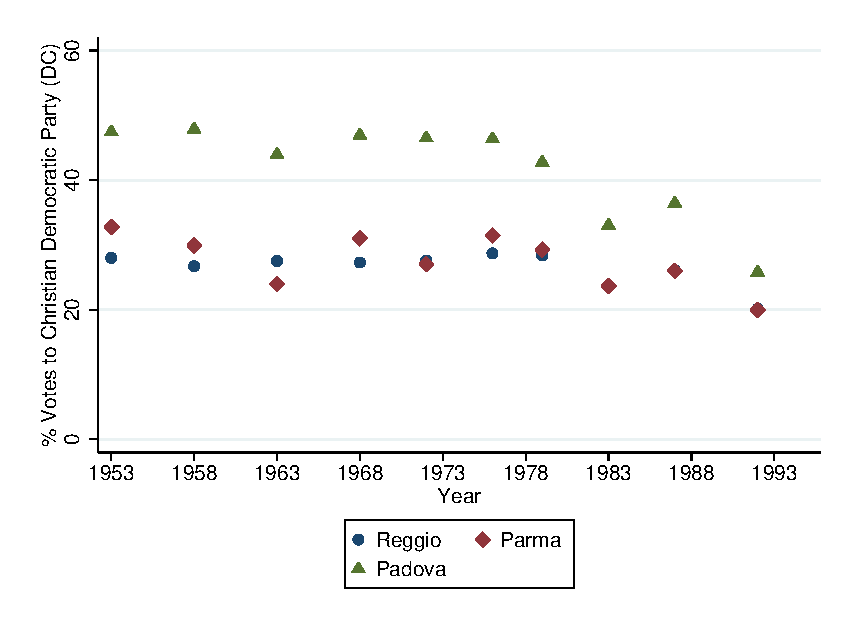
\includegraphics[width=\textwidth]{../../output/image/DC.eps}
\caption{Christian Democrats}
        \end{subfigure}
        \begin{subfigure}[t]{0.49\textwidth}
          \includegraphics[width=\textwidth]{../../output/image/PCI.eps}
 \caption{Communist Party}
        \end{subfigure}
      \caption{Election Statistics}  \label{fig:election}
    \end{figure}

    \begin{figure}[H]
    \centering
    \caption{Religious Marriages}
    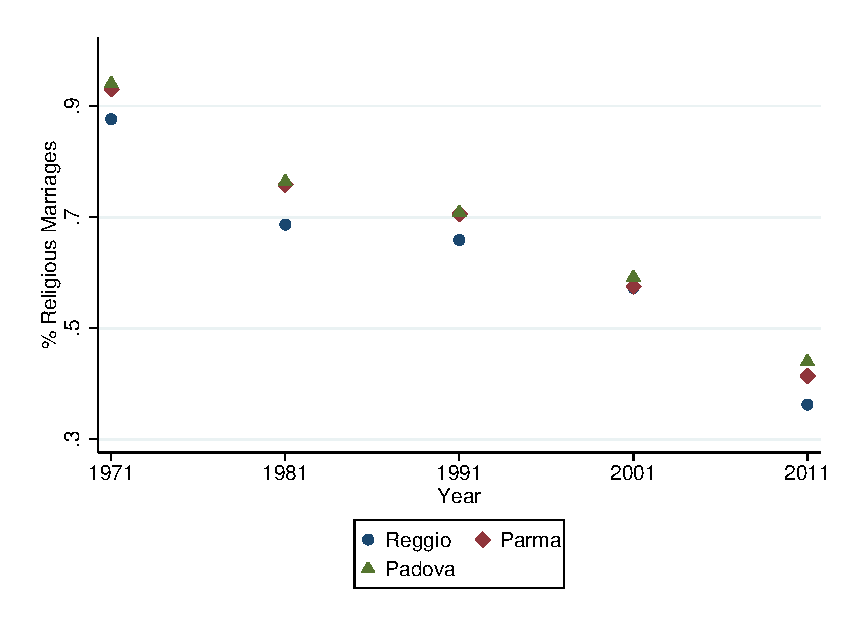
\includegraphics[width=\textwidth]{../../output/rel_mar.eps}
	\end{figure}
	
\begin{figure}[H]
      \centering
        \begin{subfigure}[t]{0.49\textwidth}
          \includegraphics[width=\textwidth]{../../output/image/enroll_num_graph.eps}
\caption{Num. of Children Enrolled in Preschool}
        \end{subfigure}
        \begin{subfigure}[t]{0.49\textwidth}
          \includegraphics[width=\textwidth]{../../output/image/enroll_per_graph.eps}
 \caption{Percentage of Ages 3-5 Enrolled in Preschool}
        \end{subfigure}
        \begin{subfigure}[t]{0.49\textwidth}
          \includegraphics[width=\textwidth]{../../output/image/enroll_per_muni_graph.eps}
        \caption{Percentage of Enrollment in Municipal Preschools}
        \end{subfigure}
        \begin{subfigure}[t]{0.49\textwidth}
          \includegraphics[width=\textwidth]{../../output/image/enroll_per_stat_graph.eps}
            \caption{Percentage of Enrollment in State Preschools}
        \end{subfigure}
      \begin{subfigure}[ht]{0.48\textwidth}
        \includegraphics[width=\textwidth]{../../output/image/enroll_per_priv_graph.eps}
        \caption{Percentage of Enrollment in Religious Preschools}
        \label{fig:large}
      \end{subfigure}
      \caption{Enrollment Statistics}  \label{fig:enrollment}
    \end{figure}    
    
    
\subsection{Sample Differences in Municipal and Municipal-Affiliated Preschools}

In this section, we test if there are differences in baseline characteristics between the sample that attends municipal preschools and the sample that attends municipal-affiliated preschools across each city. As Table \ref{tab:sample} in the main paper shows, there are only few people who attended municipal-affiliated preschools for each cell, except for the child cohorts in Parma and Padova. Since there are very few people in the adult cohorts who attended municipal-affiliated school, we decide to test the differences in baseline characteristics only for child and adolescent cohorts. 

 
    

\section{Empirical Results for Preschools (ages 3-6)}
\label{sec:results}
\subsection{Estimation Results for Reggio Approach Preschools, Comparison with Other School Types} \label{app:comparison-reli-stat}

\begin{table}[H] \caption{Estimation Results for Main Outcomes, Comparison to Religious Preschools, Child Cohort} \label{ols-M-child-reg-reli}
\scalebox{0.8}{\begin{tabular}{l c c c c c c}
\toprule
 & NoneIt & BICIt & FullIt & DidPmIt & DidPvIt & AIPWIt \\
\midrule
SDQ Composite - Child &      0.64 & \textbf{      1.03 } & \textbf{      1.29 } & \textbf{      1.26 } &     -0.73 & \textbf{     0.84} \\
& (     0.53 ) & (     0.53 ) & (     0.53 ) & (     0.79 ) & (     0.60 ) & (     0.47 ) \\
& \textit{ 315 } & \textit{ 315 } & \textit{ 315 } & \textit{ 442 } & \textit{ 577 } & \textit{ 315 } \\
Obese &      0.08 &      0.07 & \textbf{      0.10 } &      0.00 & \textbf{      0.10 } &      0.00 \\
& (     0.05 ) & (     0.06 ) & (     0.06 ) & (     0.07 ) & (     0.06 ) & (     0.06 ) \\
& \textit{ 315 } & \textit{ 315 } & \textit{ 315 } & \textit{ 442 } & \textit{ 577 } & \textit{ 315 } \\
Overweight &      0.04 &      0.05 &      0.06 &      0.06 &     -0.01 & \textbf{     0.07} \\
& (     0.04 ) & (     0.04 ) & (     0.04 ) & (     0.07 ) & (     0.04 ) & (     0.04 ) \\
& \textit{ 315 } & \textit{ 315 } & \textit{ 315 } & \textit{ 442 } & \textit{ 577 } & \textit{ 315 } \\
Health is Good &     -0.03 &     -0.03 &     -0.00 & \textbf{     -0.15 } &      0.03 &     -0.04 \\
& (     0.06 ) & (     0.06 ) & (     0.06 ) & (     0.09 ) & (     0.05 ) & (     0.06 ) \\
& \textit{ 315 } & \textit{ 315 } & \textit{ 315 } & \textit{ 442 } & \textit{ 576 } & \textit{ 315 } \\
Not Excited to Learn &      0.02 &      0.02 &      0.02 & \textbf{     -0.06 } &      0.04 & \textbf{     0.03} \\
& (     0.02 ) & (     0.02 ) & (     0.02 ) & (     0.04 ) & (     0.03 ) & (     0.01 ) \\
& \textit{ 315 } & \textit{ 315 } & \textit{ 315 } & \textit{ 442 } & \textit{ 577 } & \textit{ 315 } \\
Problems Sitting Still &     -0.01 &      0.02 &     -0.04 &      0.08 & \textbf{      0.07 } &      0.02 \\
& (     0.04 ) & (     0.04 ) & (     0.04 ) & (     0.07 ) & (     0.04 ) & (     0.05 ) \\
& \textit{ 315 } & \textit{ 315 } & \textit{ 315 } & \textit{ 442 } & \textit{ 577 } & \textit{ 315 } \\
How Much Child Likes School &      0.04 &      0.04 &      0.06 &     -0.12 &     -0.07 &      0.05 \\
& (     0.07 ) & (     0.07 ) & (     0.08 ) & (     0.09 ) & (     0.08 ) & (     0.08 ) \\
& \textit{ 314 } & \textit{ 314 } & \textit{ 314 } & \textit{ 441 } & \textit{ 576 } & \textit{ 314 } \\
\bottomrule
\end{tabular}
}
\vspace{1ex} \\
\footnotesize\raggedright{Note: This table shows the estimates of the coefficient for attending Reggio Approach preschools from multiple methods. We compare Reggio Approach individuals with those who attended religious preschools. Column title indicates the corresponding control set and and model. \textbf{None} = OLS estimate with no control variables. \textbf{BIC} = OLS estimate with controls selected by Bayesian Information Criterion (BIC) and additional controls for male indicator, migrant indicator, and ITC attendance indicator. \textbf{Full} = OLS estimate with the full set of controls. \textbf{PSM} =  propensity score matching estimation. \textbf{AIPW} = augmented inverse propensity weighting estimation. \textbf{DidPm} = difference-in-difference estimate of (Reggio Muni - Parma Muni) - (Reggio Reli - Parma Reli). \textbf{PSMPm} = propensity score matching between Reggio Approach people and people who attended Parma religious preschools. \textbf{DidPv} = difference-in-difference estimate of (Reggio Muni - Padova Muni) - (Reggio Reli - Padova Reli). \textbf{PSMPv} = propensity score matching between Reggio Approach people and people who attended Padova religious preschools. Robust standard errors are reported in parentheses. Bold number shows that the estimate is statistically significant at the 15\% level. Number of observations used in estimation is reported in italic.}
\end{table}

\begin{table}[H] \caption{Estimation Results for Main Outcomes, Comparison to State Preschools, Child Cohort} \label{ols-M-child-reg-state}
\scalebox{0.8}{\begin{tabular}{l c c c c c c}
\toprule
 & NoneIt & BICIt & FullIt & DidPmIt & DidPvIt & AIPWIt \\
\midrule
SDQ Composite - Child &      0.79 &      0.67 &      0.95 &      0.16 &      0.30 &      0.63 \\
& (     0.69 ) & (     0.66 ) & (     0.68 ) & (     0.81 ) & (     0.71 ) & (     0.60 ) \\
& \textit{ 290 } & \textit{ 290 } & \textit{ 290 } & \textit{ 392 } & \textit{ 474 } & \textit{ 290 } \\
Obese &     -0.09 &     -0.01 &     -0.05 &      0.01 &     -0.02 &      0.01 \\
& (     0.06 ) & (     0.06 ) & (     0.06 ) & (     0.08 ) & (     0.07 ) & (     0.06 ) \\
& \textit{ 290 } & \textit{ 290 } & \textit{ 290 } & \textit{ 392 } & \textit{ 474 } & \textit{ 290 } \\
Overweight & \textbf{      0.06 } &      0.03 &      0.06 &      0.10 & \textbf{     -0.09 } &      0.03 \\
& (     0.04 ) & (     0.05 ) & (     0.05 ) & (     0.07 ) & (     0.05 ) & (     0.05 ) \\
& \textit{ 290 } & \textit{ 290 } & \textit{ 290 } & \textit{ 392 } & \textit{ 474 } & \textit{ 290 } \\
Health is Good &     -0.07 &     -0.02 &     -0.00 &     -0.11 &     -0.05 &     -0.01 \\
& (     0.06 ) & (     0.07 ) & (     0.07 ) & (     0.09 ) & (     0.06 ) & (     0.07 ) \\
& \textit{ 290 } & \textit{ 290 } & \textit{ 290 } & \textit{ 392 } & \textit{ 474 } & \textit{ 290 } \\
Not Excited to Learn &     -0.04 &     -0.02 &     -0.02 &     -0.02 &      0.03 &     -0.01 \\
& (     0.03 ) & (     0.03 ) & (     0.04 ) & (     0.04 ) & (     0.03 ) & (     0.03 ) \\
& \textit{ 290 } & \textit{ 290 } & \textit{ 290 } & \textit{ 392 } & \textit{ 474 } & \textit{ 290 } \\
Problems Sitting Still &      0.05 &      0.06 &      0.04 & \textbf{      0.13 } & \textbf{      0.09 } &      0.04 \\
& (     0.04 ) & (     0.05 ) & (     0.05 ) & (     0.07 ) & (     0.04 ) & (     0.05 ) \\
& \textit{ 290 } & \textit{ 290 } & \textit{ 290 } & \textit{ 392 } & \textit{ 474 } & \textit{ 290 } \\
How Much Child Likes School &     -0.01 &     -0.08 &     -0.04 &     -0.08 &     -0.10 &     -0.03 \\
& (     0.08 ) & (     0.09 ) & (     0.09 ) & (     0.10 ) & (     0.09 ) & (     0.08 ) \\
& \textit{ 290 } & \textit{ 290 } & \textit{ 290 } & \textit{ 392 } & \textit{ 474 } & \textit{ 290 } \\
\bottomrule
\end{tabular}
}
\vspace{1ex} \\
\footnotesize\raggedright{Note: This table shows the estimates of the coefficient for attending Reggio Approach preschools from multiple methods. We compare Reggio Approach individuals with those who attended state preschools. Column title indicates the corresponding control set and and model. \textbf{None} = OLS estimate with no control variables. \textbf{BIC} = OLS estimate with controls selected by Bayesian Information Criterion (BIC) and additional controls for male indicator, migrant indicator, and ITC attendance indicator. \textbf{Full} = OLS estimate with the full set of controls. \textbf{PSM} =  propensity score matching estimation. \textbf{AIPW} = augmented inverse propensity weighting estimation. \textbf{DidPm} = difference-in-difference estimate of (Reggio Muni - Parma Muni) - (Reggio State - Parma State). \textbf{PSMPm} = propensity score matching between Reggio Approach people and people who attended Parma state preschools. \textbf{DidPv} = difference-in-difference estimate of (Reggio Muni - Padova Muni) - (Reggio State - Padova State). \textbf{PSMPv} = propensity score matching between Reggio Approach people and people who attended Padova state preschools. Robust standard errors are reported in parentheses. Bold number shows that the estimate is statistically significant at the 15\% level. Number of observations used in estimation is reported in italic.}

\end{table}


\begin{table}[H] \caption{Estimation Results for Main Outcomes, Comparison to Religious Preschools, Adolescent Cohort} \label{ols-M-adol-reg-reli}
\scalebox{0.8}{\begin{tabular}{l c c c c c c c c c}
\toprule
 & None & Bic & Full & PSM & AIPW & DidPm & PSMPm & DidPv & PSMPv \\
\midrule
IQ Factor & -0.13 & \textbf{ -0.15 } & -0.07 & \textbf{-0.16} & -0.18 & -0.10 & 0.04 & -0.10 & 0.14 \\
& (0.10) & (0.10) & (0.11) & (0.10) & (0.08) & (0.15) & (0.16) & (0.18) & (0.14) \\
& \textit{ 251 } & \textit{ 251 } & \textit{ 251 } & \textit{ 251 } & \textit{ 251 } & \textit{ 433 } & \textit{ 238 } & \textit{ 467 } & \textit{ 288 } \\
SDQ Composite - Child & 0.55 & 0.82 & \textbf{ 1.25 } & 0.36 & 0.90 & -0.56 & \textbf{2.84} & 0.16 & 1.05 \\
& (0.70) & (0.79) & (0.76) & (1.03) & (0.75) & (1.05) & (1.47) & (0.91) & (0.82) \\
& \textit{ 251 } & \textit{ 251 } & \textit{ 251 } & \textit{ 251 } & \textit{ 251 } & \textit{ 433 } & \textit{ 238 } & \textit{ 463 } & \textit{ 286 } \\
SDQ Composite & \textbf{ 1.44 } & \textbf{ 1.74 } & \textbf{ 1.54 } & \textbf{1.96} & \textbf{1.68} & 0.68 & 0.78 & 0.81 & \textbf{2.16} \\
& (0.70) & (0.78) & (0.82) & (1.04) & (0.76) & (1.01) & (1.10) & (1.03) & (1.15) \\
& \textit{ 249 } & \textit{ 249 } & \textit{ 249 } & \textit{ 249 } & \textit{ 249 } & \textit{ 429 } & \textit{ 235 } & \textit{ 463 } & \textit{ 286 } \\
Depression Score - positive & \textbf{ 1.89 } & \textbf{ 2.97 } & \textbf{ 2.34 } & \textbf{2.84} & \textbf{2.88} & 1.47 & \textbf{1.93} & \textbf{ 1.87 } & 1.84 \\
& (0.88) & (0.96) & (1.02) & (1.12) & (0.87) & (1.17) & (0.93) & (1.24) & (1.15) \\
& \textit{ 245 } & \textit{ 245 } & \textit{ 245 } & \textit{ 245 } & \textit{ 245 } & \textit{ 418 } & \textit{ 230 } & \textit{ 459 } & \textit{ 283 } \\
Locus of Control - positive & 0.08 & \textbf{ 0.16 } & 0.09 & \textbf{0.23} & \textbf{0.13} & -0.04 & \textbf{0.26} & 0.19 & 0.31 \\
& (0.09) & (0.10) & (0.10) & (0.09) & (0.11) & (0.15) & (0.12) & (0.14) & (0.19) \\
& \textit{ 248 } & \textit{ 248 } & \textit{ 248 } & \textit{ 248 } & \textit{ 248 } & \textit{ 426 } & \textit{ 233 } & \textit{ 462 } & \textit{ 285 } \\
Not Obese & \textbf{ -0.11 } & \textbf{ -0.12 } & \textbf{ -0.10 } & \textbf{-0.08} & -0.11 & 0.01 & \textbf{-0.14} & -0.06 & 0.07 \\
& (0.04) & (0.05) & (0.05) & (0.05) & (0.05) & (0.06) & (0.04) & (0.07) & (0.08) \\
& \textit{ 251 } & \textit{ 251 } & \textit{ 251 } & \textit{ 251 } & \textit{ 251 } & \textit{ 433 } & \textit{ 238 } & \textit{ 467 } & \textit{ 288 } \\
Not Overweight & 0.00 & -0.02 & -0.02 & -0.04 & -0.01 & \textbf{ 0.08 } & \textbf{-0.04} & -0.03 & -0.04 \\
& (0.02) & (0.03) & (0.03) & (0.05) & (0.03) & (0.04) & (0.02) & (0.03) & (0.03) \\
& \textit{ 251 } & \textit{ 251 } & \textit{ 251 } & \textit{ 251 } & \textit{ 251 } & \textit{ 433 } & \textit{ 238 } & \textit{ 467 } & \textit{ 288 } \\
Health is Good & 0.04 & 0.05 & 0.06 & -0.03 & 0.04 & \textbf{ 0.18 } & 0.02 & 0.07 & 0.06 \\
& (0.06) & (0.07) & (0.07) & (0.07) & (0.07) & (0.10) & (0.07) & (0.09) & (0.10) \\
& \textit{ 250 } & \textit{ 250 } & \textit{ 250 } & \textit{ 250 } & \textit{ 250 } & \textit{ 432 } & \textit{ 238 } & \textit{ 466 } & \textit{ 288 } \\
Go To School & 0.03 & 0.01 & 0.02 & -0.02 & 0.00 & 0.03 & 0.00 & 0.04 & -0.04 \\
& (0.03) & (0.02) & (0.03) & (0.03) & (0.03) & (0.04) & (0.04) & (0.03) & (0.03) \\
& \textit{ 251 } & \textit{ 251 } & \textit{ 251 } & \textit{ 251 } & \textit{ 251 } & \textit{ 433 } & \textit{ 238 } & \textit{ 467 } & \textit{ 288 } \\
How Much Child Likes School & -0.09 & -0.03 & -0.12 & -0.01 & 0.00 & -0.15 & \textbf{0.44} & -0.07 & 0.05 \\
& (0.12) & (0.13) & (0.13) & (0.14) & (0.15) & (0.18) & (0.25) & (0.17) & (0.17) \\
& \textit{ 240 } & \textit{ 240 } & \textit{ 240 } & \textit{ 240 } & \textit{ 240 } & \textit{ 414 } & \textit{ 230 } & \textit{ 453 } & \textit{ 282 } \\
Days of Sport (Weekly) & -0.25 & -0.33 & -0.07 & -0.41 & -0.32 & -0.35 & \textbf{-1.01} & -0.43 & -0.38 \\
& (0.25) & (0.29) & (0.29) & (0.42) & (0.27) & (0.37) & (0.53) & (0.37) & (0.46) \\
& \textit{ 246 } & \textit{ 246 } & \textit{ 246 } & \textit{ 246 } & \textit{ 246 } & \textit{ 420 } & \textit{ 232 } & \textit{ 449 } & \textit{ 278 } \\
Num. of Friends & -0.06 & 0.02 & 0.29 & 0.08 & 0.44 & -0.77 & -2.19 & -0.28 & 0.05 \\
& (1.39) & (1.11) & (1.30) & (1.30) & (1.08) & (2.13) & (2.10) & (2.26) & (1.62) \\
& \textit{ 245 } & \textit{ 245 } & \textit{ 245 } & \textit{ 245 } & \textit{ 245 } & \textit{ 414 } & \textit{ 227 } & \textit{ 418 } & \textit{ 259 } \\
Volunteers & -0.03 & 0.03 & 0.03 & -0.02 & 0.01 & -0.01 & \textbf{0.26} & -0.03 & 0.06 \\
& (0.06) & (0.07) & (0.07) & (0.08) & (0.08) & (0.09) & (0.07) & (0.09) & (0.09) \\
& \textit{ 251 } & \textit{ 251 } & \textit{ 251 } & \textit{ 251 } & \textit{ 251 } & \textit{ 433 } & \textit{ 238 } & \textit{ 467 } & \textit{ 288 } \\
Trust Score & -0.00 & 0.10 & 0.01 & 0.23 & 0.13 & 0.10 & -0.59 & -0.07 & 0.13 \\
& (0.19) & (0.22) & (0.22) & (0.30) & (0.23) & (0.29) & (0.48) & (0.28) & (0.26) \\
& \textit{ 249 } & \textit{ 249 } & \textit{ 249 } & \textit{ 249 } & \textit{ 249 } & \textit{ 429 } & \textit{ 235 } & \textit{ 460 } & \textit{ 282 } \\
\bottomrule
\end{tabular}
}
\vspace{1ex} \\
\footnotesize\raggedright{Note: This table shows the estimates of the coefficient for attending Reggio Approach preschools from multiple methods. We compare Reggio Approach individuals with those who attended religious preschools. Column title indicates the corresponding control set and and model. \textbf{None} = OLS estimate with no control variables. \textbf{BIC} = OLS estimate with controls selected by Bayesian Information Criterion (BIC) and additional controls for male indicator, migrant indicator, and ITC attendance indicator. \textbf{Full} = OLS estimate with the full set of controls. \textbf{PSM} =  propensity score matching estimation. \textbf{AIPW} = augmented inverse propensity weighting estimation. \textbf{DidPm} = difference-in-difference estimate of (Reggio Muni - Parma Muni) - (Reggio Reli - Parma Reli). \textbf{PSMPm} = propensity score matching between Reggio Approach people and people who attended Parma religious preschools. \textbf{DidPv} = difference-in-difference estimate of (Reggio Muni - Padova Muni) - (Reggio Reli - Padova Reli). \textbf{PSMPv} = propensity score matching between Reggio Approach people and people who attended Padova religious preschools. Robust standard errors are reported in parentheses. Bold number shows that the estimate is statistically significant at the 15\% level. Number of observations used in estimation is reported in italic.}
\end{table}

\begin{table}[H] \caption{Estimation Results for Main Outcomes, Comparison to State Preschools, Adolescent Cohort} \label{ols-M-adol-reg-stat}
\scalebox{0.8}{\begin{tabular}{l c c c c c c}
\toprule
 & None & Bic & Full & AIPW & DidPm & DidPv \\
\midrule
IQ Score &     -0.02 &     -0.05 &      0.01 & \textbf{     0.13} &     -0.07 & \textbf{     -0.21 } \\
& (     0.05 ) & (     0.06 ) & (     0.06 ) & (     0.13 ) & (     0.07 ) & (     0.09 ) \\
& \textit{ 185 } & \textit{ 185 } & \textit{ 185 } & \textit{ 185 } & \textit{ 275 } & \textit{ 316 } \\
IQ Factor &     -0.07 &     -0.20 &      0.02 &      0.42 &     -0.15 & \textbf{     -0.79 } \\
& (     0.18 ) & (     0.22 ) & (     0.23 ) & (     0.48 ) & (     0.25 ) & (     0.30 ) \\
& \textit{ 185 } & \textit{ 185 } & \textit{ 185 } & \textit{ 185 } & \textit{ 275 } & \textit{ 316 } \\
SDQ Composite - Child & \textbf{     -2.09 } & \textbf{     -2.18 } & \textbf{     -1.61 } &     -0.88 &     -1.09 & \textbf{     -3.08 } \\
& (     0.62 ) & (     0.79 ) & (     0.70 ) & (     1.21 ) & (     1.17 ) & (     1.06 ) \\
& \textit{ 185 } & \textit{ 185 } & \textit{ 185 } & \textit{ 185 } & \textit{ 275 } & \textit{ 313 } \\
SDQ Composite &     -1.02 &     -1.15 &     -1.32 &     -3.29 &      0.48 &     -0.15 \\
& (     1.00 ) & (     1.03 ) & (     1.11 ) & (     1.91 ) & (     1.48 ) & (     1.32 ) \\
& \textit{ 183 } & \textit{ 183 } & \textit{ 183 } & \textit{ 183 } & \textit{ 273 } & \textit{ 312 } \\
Depression Score - positive &      0.09 &      0.64 &      0.36 &     -3.32 & \textbf{      2.90 } & \textbf{      2.92 } \\
& (     1.25 ) & (     1.38 ) & (     1.43 ) & (     3.23 ) & (     1.62 ) & (     1.66 ) \\
& \textit{ 180 } & \textit{ 180 } & \textit{ 180 } & \textit{ 180 } & \textit{ 266 } & \textit{ 308 } \\
Locus of Control - positive &     -0.14 &     -0.06 &     -0.07 &     -0.44 & \textbf{     -0.61 } &     -0.08 \\
& (     0.14 ) & (     0.16 ) & (     0.17 ) & (     0.25 ) & (     0.23 ) & (     0.20 ) \\
& \textit{ 182 } & \textit{ 182 } & \textit{ 182 } & \textit{ 182 } & \textit{ 271 } & \textit{ 311 } \\
Obese &     -0.03 &      0.08 &      0.01 &      0.01 &     -0.07 & \textbf{      0.24 } \\
& (     0.08 ) & (     0.08 ) & (     0.08 ) & (     0.18 ) & (     0.10 ) & (     0.12 ) \\
& \textit{ 185 } & \textit{ 185 } & \textit{ 185 } & \textit{ 185 } & \textit{ 275 } & \textit{ 316 } \\
Overweight &     -0.04 &      0.00 &     -0.02 &      0.06 & \textbf{     -0.14 } &     -0.00 \\
& (     0.05 ) & (     0.05 ) & (     0.05 ) & (     0.05 ) & (     0.08 ) & (     0.06 ) \\
& \textit{ 185 } & \textit{ 185 } & \textit{ 185 } & \textit{ 185 } & \textit{ 275 } & \textit{ 316 } \\
Health is Good &      0.05 &      0.07 &      0.10 &      0.03 &      0.01 & \textbf{      0.28 } \\
& (     0.10 ) & (     0.10 ) & (     0.11 ) & (     0.36 ) & (     0.15 ) & (     0.13 ) \\
& \textit{ 185 } & \textit{ 185 } & \textit{ 185 } & \textit{ 185 } & \textit{ 275 } & \textit{ 316 } \\
Go To School &      0.05 &      0.02 &      0.04 &     -0.01 &      0.04 &      0.02 \\
& (     0.05 ) & (     0.05 ) & (     0.06 ) & (     0.21 ) & (     0.05 ) & (     0.06 ) \\
& \textit{ 185 } & \textit{ 185 } & \textit{ 185 } & \textit{ 185 } & \textit{ 275 } & \textit{ 316 } \\
How Much Child Likes School &     -0.24 &     -0.29 & \textbf{     -0.41 } &      0.18 &     -0.08 &     -0.34 \\
& (     0.20 ) & (     0.22 ) & (     0.20 ) & (     0.96 ) & (     0.27 ) & (     0.26 ) \\
& \textit{ 178 } & \textit{ 178 } & \textit{ 178 } & \textit{ 178 } & \textit{ 268 } & \textit{ 305 } \\
Days of Sport (Weekly) & \textbf{     -0.87 } & \textbf{     -1.14 } & \textbf{     -0.95 } &     -1.17 & \textbf{     -1.59 } & \textbf{     -0.95 } \\
& (     0.38 ) & (     0.42 ) & (     0.43 ) & (     1.21 ) & (     0.54 ) & (     0.53 ) \\
& \textit{ 180 } & \textit{ 180 } & \textit{ 180 } & \textit{ 180 } & \textit{ 268 } & \textit{ 299 } \\
\bottomrule
\end{tabular}
}
\vspace{1ex} \\
\footnotesize\raggedright{Note: This table shows the estimates of the coefficient for attending Reggio Approach preschools from multiple methods. We compare Reggio Approach individuals with those who attended state preschools. Column title indicates the corresponding control set and and model. \textbf{None} = OLS estimate with no control variables. \textbf{BIC} = OLS estimate with controls selected by Bayesian Information Criterion (BIC) and additional controls for male indicator, migrant indicator, and ITC attendance indicator. \textbf{Full} = OLS estimate with the full set of controls. \textbf{PSM} =  propensity score matching estimation. \textbf{AIPW} = augmented inverse propensity weighting estimation. \textbf{DidPm} = difference-in-difference estimate of (Reggio Muni - Parma Muni) - (Reggio State - Parma State). \textbf{PSMPm} = propensity score matching between Reggio Approach people and people who attended Parma state preschools. \textbf{DidPv} = difference-in-difference estimate of (Reggio Muni - Padova Muni) - (Reggio State - Padova State). \textbf{PSMPv} = propensity score matching between Reggio Approach people and people who attended Padova state preschools. Robust standard errors are reported in parentheses. Bold number shows that the estimate is statistically significant at the 15\% level. Number of observations used in estimation is reported in italic.}
\end{table}


\begin{table}[H] \caption{Estimation Results for Main Outcomes, Comparison to Religious Preschools, Age-30 Cohort} \label{ols-M-adult30-reg-reli}
\scalebox{0.75}{\begin{tabular}{l c c c c c c c c c}
\toprule
 & None & BIC & Full & PSM & AIPW & DidPm & PSMPm & DidPv & PSMPv \\
\midrule
IQ Factor & \textbf{ -0.42 } & \textbf{ -0.41 } & \textbf{ -0.36 } & \textbf{-0.46} & -0.47 & \textbf{ -0.63 } & \textbf{-0.69} & -0.19 & \textbf{-0.84} \\
& (0.15) & (0.17) & (0.18) & (0.17) & (0.17) & (0.20) & (0.12) & (0.23) & (0.12) \\
& \textit{ 144 } & \textit{ 144 } & \textit{ 144 } & \textit{ 144 } & \textit{ 144 } & \textit{ 227 } & \textit{ 151 } & \textit{ 289 } & \textit{ 236 } \\
Graduate from High School & -0.02 & -0.00 & -0.02 & -0.06 & 0.03 & 0.06 & \textbf{-0.10} & -0.10 & 0.03 \\
& (0.06) & (0.06) & (0.07) & (0.12) & (0.08) & (0.09) & (0.03) & (0.08) & (0.05) \\
& \textit{ 144 } & \textit{ 144 } & \textit{ 144 } & \textit{ 144 } & \textit{ 144 } & \textit{ 227 } & \textit{ 151 } & \textit{ 289 } & \textit{ 236 } \\
High School Grade & \textbf{ 3.11 } & 2.44 & 2.37 & \textbf{2.91} & 1.70 & 4.74 & \textbf{7.17} & 2.24 & \textbf{5.61} \\
& (1.61) & (1.69) & (1.82) & (1.42) & (1.95) & (3.47) & (2.00) & (3.84) & (2.59) \\
& \textit{ 112 } & \textit{ 112 } & \textit{ 112 } & \textit{ 112 } & \textit{ 112 } & \textit{ 186 } & \textit{ 121 } & \textit{ 229 } & \textit{ 182 } \\
High School Grade (Standardized) & \textbf{ 4.38 } & 3.29 & \textbf{ 4.05 } & \textbf{4.15} & 2.29 & \textbf{ 5.11 } & \textbf{3.01} & 3.66 & 2.15 \\
& (2.24) & (2.37) & (2.24) & (1.49) & (2.20) & (3.07) & (1.74) & (4.42) & (3.02) \\
& \textit{ 112 } & \textit{ 112 } & \textit{ 112 } & \textit{ 112 } & \textit{ 112 } & \textit{ 184 } & \textit{ 120 } & \textit{ 227 } & \textit{ 181 } \\
Max Edu: University & 0.09 & 0.08 & 0.04 & 0.07 & 0.03 & \textbf{ 0.20 } & \textbf{-0.25} & \textbf{ 0.26 } & \textbf{-0.25} \\
& (0.07) & (0.07) & (0.09) & (0.07) & (0.13) & (0.13) & (0.10) & (0.14) & (0.08) \\
& \textit{ 144 } & \textit{ 144 } & \textit{ 144 } & \textit{ 144 } & \textit{ 144 } & \textit{ 227 } & \textit{ 151 } & \textit{ 289 } & \textit{ 236 } \\
Employed & \textbf{ -0.06 } & \textbf{ -0.06 } & \textbf{ -0.04 } & \textbf{-0.06} & -0.06 & 0.08 & -0.03 & -0.09 & 0.04 \\
& (0.02) & (0.03) & (0.02) & (0.02) & (0.02) & (0.08) & (0.03) & (0.08) & (0.04) \\
& \textit{ 144 } & \textit{ 144 } & \textit{ 144 } & \textit{ 144 } & \textit{ 144 } & \textit{ 227 } & \textit{ 151 } & \textit{ 289 } & \textit{ 236 } \\
Hours Worked Per Week & -2.09 & -2.16 & -2.38 & -2.25 & -2.56 & 1.13 & 1.67 & -2.23 & 1.04 \\
& (1.62) & (1.70) & (1.74) & (1.80) & (1.65) & (4.06) & (3.05) & (3.95) & (2.78) \\
& \textit{ 125 } & \textit{ 125 } & \textit{ 125 } & \textit{ 125 } & \textit{ 125 } & \textit{ 205 } & \textit{ 131 } & \textit{ 267 } & \textit{ 214 } \\
Married or Cohabitating & 0.01 & 0.04 & 0.06 & -0.13 & -0.05 & 0.11 & -0.18 & 0.17 & \textbf{-0.17} \\
& (0.09) & (0.10) & (0.11) & (0.13) & (0.11) & (0.14) & (0.11) & (0.15) & (0.07) \\
& \textit{ 144 } & \textit{ 144 } & \textit{ 144 } & \textit{ 144 } & \textit{ 144 } & \textit{ 227 } & \textit{ 151 } & \textit{ 289 } & \textit{ 236 } \\
Not Obese & \textbf{ -0.12 } & -0.10 & -0.06 & -0.11 & -0.12 & \textbf{ -0.18 } & -0.08 & -0.12 & \textbf{-0.17} \\
& (0.07) & (0.07) & (0.08) & (0.08) & (0.10) & (0.12) & (0.09) & (0.12) & (0.07) \\
& \textit{ 144 } & \textit{ 144 } & \textit{ 144 } & \textit{ 144 } & \textit{ 144 } & \textit{ 227 } & \textit{ 151 } & \textit{ 289 } & \textit{ 236 } \\
Not Overweight & -0.01 & 0.01 & -0.02 & -0.02 & 0.02 & 0.13 & -0.02 & -0.04 & 0.03 \\
& (0.08) & (0.08) & (0.09) & (0.07) & (0.10) & (0.12) & (0.08) & (0.12) & (0.05) \\
& \textit{ 144 } & \textit{ 144 } & \textit{ 144 } & \textit{ 144 } & \textit{ 144 } & \textit{ 227 } & \textit{ 151 } & \textit{ 289 } & \textit{ 236 } \\
Locus of Control - positive & -0.11 & -0.04 & -0.12 & 0.08 & -0.03 & \textbf{ 0.49 } & -0.24 & 0.20 & \textbf{-0.41} \\
& (0.16) & (0.14) & (0.17) & (0.18) & (0.17) & (0.25) & (0.15) & (0.24) & (0.11) \\
& \textit{ 139 } & \textit{ 139 } & \textit{ 139 } & \textit{ 139 } & \textit{ 139 } & \textit{ 216 } & \textit{ 145 } & \textit{ 278 } & \textit{ 229 } \\
Depression Score - positive & \textbf{ -1.83 } & -1.01 & -1.04 & -1.57 & -0.98 & -0.65 & \textbf{-1.88} & -0.14 & \textbf{-3.69} \\
& (1.08) & (0.84) & (0.92) & (1.50) & (1.12) & (1.38) & (0.83) & (1.73) & (0.70) \\
& \textit{ 142 } & \textit{ 142 } & \textit{ 142 } & \textit{ 142 } & \textit{ 142 } & \textit{ 225 } & \textit{ 150 } & \textit{ 285 } & \textit{ 234 } \\
Ever Voted for Municipal & \textbf{ -0.16 } & -0.03 & -0.04 & 0.03 & 0.04 & -0.03 & \textbf{0.16} & \textbf{ 0.21 } & -0.07 \\
& (0.10) & (0.07) & (0.09) & (0.06) & (0.07) & (0.11) & (0.09) & (0.12) & (0.07) \\
& \textit{ 142 } & \textit{ 142 } & \textit{ 142 } & \textit{ 142 } & \textit{ 142 } & \textit{ 224 } & \textit{ 150 } & \textit{ 277 } & \textit{ 228 } \\
Ever Voted for Regional & \textbf{ -0.16 } & -0.04 & -0.06 & 0.00 & -0.00 & -0.03 & \textbf{0.21} & \textbf{ 0.29 } & -0.07 \\
& (0.10) & (0.07) & (0.09) & (0.05) & (0.07) & (0.10) & (0.07) & (0.12) & (0.08) \\
& \textit{ 142 } & \textit{ 142 } & \textit{ 142 } & \textit{ 142 } & \textit{ 142 } & \textit{ 224 } & \textit{ 150 } & \textit{ 277 } & \textit{ 228 } \\
\bottomrule
\end{tabular}
}
\vspace{1ex} \\
\footnotesize\raggedright{Note: This table shows the estimates of the coefficient for attending Reggio Approach preschools from multiple methods. We compare Reggio Approach individuals with those who attended religious preschools. Column title indicates the corresponding control set and and model. \textbf{None} = OLS estimate with no control variables. \textbf{BIC} = OLS estimate with controls selected by Bayesian Information Criterion (BIC) and additional controls for male indicator, migrant indicator, and ITC attendance indicator. \textbf{Full} = OLS estimate with the full set of controls. \textbf{PSM} =  propensity score matching estimation. \textbf{AIPW} = augmented inverse propensity weighting estimation. \textbf{DidPm} = difference-in-difference estimate of (Reggio Muni - Parma Muni) - (Reggio Reli - Parma Reli). \textbf{PSMPm} = propensity score matching between Reggio Approach people and people who attended Parma religious preschools. \textbf{DidPv} = difference-in-difference estimate of (Reggio Muni - Padova Muni) - (Reggio Reli - Padova Reli). \textbf{PSMPv} = propensity score matching between Reggio Approach people and people who attended Padova religious preschools. Robust standard errors are reported in parentheses. Bold number shows that the estimate is statistically significant at the 15\% level. Number of observations used in estimation is reported in italic.}
\end{table}

\begin{table}[H] \caption{Estimation Results for Main Outcomes, Comparison to State Preschools, Age-30 Cohort} \label{ols-M-adult30-reg-stat}
\scalebox{0.75}{\begin{tabular}{l c c c c c c c c c}
\toprule
 & None & BIC & Full & PSM & AIPW & DidPm & PSMPm & DidPv & PSMPv \\
\midrule
IQ Factor & \textbf{ 0.64 } & \textbf{ 0.45 } & \textbf{ 0.44 } & 0.29 & \textbf{0.55} & 0.16 & \textbf{-0.49} & 0.38 & \textbf{-0.71} \\
& (0.23) & (0.18) & (0.19) & (0.18) & (0.21) & (0.26) & (0.15) & (0.33) & (0.13) \\
& \textit{ 133 } & \textit{ 133 } & \textit{ 133 } & \textit{ 133 } & \textit{ 133 } & \textit{ 218 } & \textit{ 153 } & \textit{ 173 } & \textit{ 132 } \\
Graduate from High School & \textbf{ -0.14 } & \textbf{ -0.10 } & \textbf{ -0.11 } & \textbf{-0.12} & -0.13 & -0.00 & 0.07 & \textbf{ -0.14 } & -0.10 \\
& (0.03) & (0.04) & (0.05) & (0.03) & (0.03) & (0.08) & (0.09) & (0.09) & (0.06) \\
& \textit{ 133 } & \textit{ 133 } & \textit{ 133 } & \textit{ 133 } & \textit{ 133 } & \textit{ 218 } & \textit{ 153 } & \textit{ 173 } & \textit{ 132 } \\
High School Grade & -2.59 & -2.08 & -1.64 & 1.64 & -0.29 & -1.08 & \textbf{5.76} & -1.40 & \\
& (2.36) & (2.25) & (2.51) & (1.90) & (1.98) & (4.74) & (2.77) & (5.21) & () \\
& \textit{ 99 } & \textit{ 99 } & \textit{ 99 } & \textit{ 99 } & \textit{ 99 } & \textit{ 173 } & \textit{ 121 } & \textit{ 129 } & \\
High School Grade (Standardized) & -0.23 & -0.04 & -1.14 & \textbf{4.54} & 2.05 & 2.06 & 0.47 & -0.60 & \\
& (2.59) & (2.50) & (2.81) & (1.93) & (2.04) & (3.65) & (2.33) & (5.25) & () \\
& \textit{ 98 } & \textit{ 98 } & \textit{ 98 } & \textit{ 98 } & \textit{ 98 } & \textit{ 169 } & \textit{ 119 } & \textit{ 127 } & \\
Max Edu: University & -0.10 & -0.07 & -0.02 & -0.00 & -0.14 & -0.08 & -0.12 & 0.10 & -0.15 \\
& (0.10) & (0.11) & (0.11) & (0.09) & (0.13) & (0.15) & (0.08) & (0.19) & (0.22) \\
& \textit{ 133 } & \textit{ 133 } & \textit{ 133 } & \textit{ 133 } & \textit{ 133 } & \textit{ 218 } & \textit{ 153 } & \textit{ 173 } & \textit{ 132 } \\
Employed & 0.02 & 0.01 & -0.02 & 0.01 & 0.06 & \textbf{ 0.16 } & \textbf{-0.05} & 0.11 & \textbf{-0.06} \\
& (0.06) & (0.07) & (0.07) & (0.08) & (0.10) & (0.09) & (0.03) & (0.10) & (0.02) \\
& \textit{ 133 } & \textit{ 133 } & \textit{ 133 } & \textit{ 133 } & \textit{ 133 } & \textit{ 218 } & \textit{ 153 } & \textit{ 173 } & \textit{ 132 } \\
Hours Worked Per Week & 5.65 & \textbf{ 6.06 } & 5.20 & \textbf{11.40} & \textbf{11.54} & \textbf{ 10.18 } & -2.13 & \textbf{ 8.42 } & -2.31 \\
& (4.47) & (4.16) & (4.13) & (4.38) & (5.23) & (4.96) & (2.28) & (5.29) & (2.99) \\
& \textit{ 103 } & \textit{ 103 } & \textit{ 103 } & \textit{ 103 } & \textit{ 103 } & \textit{ 186 } & \textit{ 134 } & \textit{ 142 } & \textit{ 112 } \\
Married or Cohabitating & \textbf{ 0.16 } & 0.07 & 0.02 & 0.02 & 0.08 & 0.18 & -0.03 & 0.10 & -0.22 \\
& (0.09) & (0.09) & (0.10) & (0.13) & (0.13) & (0.14) & (0.12) & (0.19) & (0.23) \\
& \textit{ 133 } & \textit{ 133 } & \textit{ 133 } & \textit{ 133 } & \textit{ 133 } & \textit{ 218 } & \textit{ 153 } & \textit{ 173 } & \textit{ 132 } \\
Not Obese & \textbf{ 0.21 } & \textbf{ 0.11 } & 0.10 & 0.02 & \textbf{0.13} & 0.15 & \textbf{-0.24} & 0.21 & \textbf{-0.27} \\
& (0.11) & (0.07) & (0.07) & (0.06) & (0.06) & (0.11) & (0.05) & (0.15) & (0.05) \\
& \textit{ 133 } & \textit{ 133 } & \textit{ 133 } & \textit{ 133 } & \textit{ 133 } & \textit{ 218 } & \textit{ 153 } & \textit{ 173 } & \textit{ 132 } \\
Not Overweight & -0.12 & -0.02 & 0.01 & -0.05 & -0.13 & 0.04 & -0.03 & 0.01 & \textbf{-0.12} \\
& (0.08) & (0.09) & (0.09) & (0.11) & (0.09) & (0.13) & (0.10) & (0.14) & (0.07) \\
& \textit{ 133 } & \textit{ 133 } & \textit{ 133 } & \textit{ 133 } & \textit{ 133 } & \textit{ 218 } & \textit{ 153 } & \textit{ 173 } & \textit{ 132 } \\
Locus of Control - positive & \textbf{ 0.40 } & \textbf{ 0.22 } & 0.22 & \textbf{0.28} & \textbf{0.28} & 0.30 & \textbf{0.29} & 0.00 & 0.27 \\
& (0.15) & (0.14) & (0.15) & (0.15) & (0.16) & (0.26) & (0.17) & (0.29) & (0.33) \\
& \textit{ 130 } & \textit{ 130 } & \textit{ 130 } & \textit{ 130 } & \textit{ 130 } & \textit{ 210 } & \textit{ 148 } & \textit{ 168 } & \textit{ 129 } \\
Depression Score - positive & \textbf{ 3.04 } & 1.11 & 1.34 & -0.39 & 0.88 & \textbf{ 2.91 } & \textbf{-4.74} & -1.29 & \textbf{-1.69} \\
& (1.58) & (0.97) & (1.02) & (0.83) & (1.23) & (1.76) & (1.42) & (2.27) & (0.90) \\
& \textit{ 132 } & \textit{ 132 } & \textit{ 132 } & \textit{ 132 } & \textit{ 132 } & \textit{ 217 } & \textit{ 152 } & \textit{ 171 } & \textit{ 131 } \\
Ever Voted for Municipal & 0.07 & -0.01 & 0.04 & -0.08 & -0.01 & -0.07 & 0.12 & \textbf{ 0.43 } & -0.18 \\
& (0.11) & (0.09) & (0.09) & (0.09) & (0.11) & (0.12) & (0.10) & (0.16) & (0.13) \\
& \textit{ 132 } & \textit{ 132 } & \textit{ 132 } & \textit{ 132 } & \textit{ 132 } & \textit{ 215 } & \textit{ 151 } & \textit{ 169 } & \textit{ 131 } \\
Ever Voted for Regional & -0.02 & -0.10 & -0.04 & -0.15 & -0.11 & -0.09 & 0.14 & \textbf{ 0.41 } & -0.16 \\
& (0.12) & (0.10) & (0.10) & (0.11) & (0.12) & (0.13) & (0.11) & (0.16) & (0.14) \\
& \textit{ 132 } & \textit{ 132 } & \textit{ 132 } & \textit{ 132 } & \textit{ 132 } & \textit{ 215 } & \textit{ 151 } & \textit{ 169 } & \textit{ 131 } \\
\bottomrule
\end{tabular}
}
\vspace{1ex} \\
\footnotesize\raggedright{Note: This table shows the estimates of the coefficient for attending Reggio Approach preschools from multiple methods. We compare Reggio Approach individuals with those who attended state preschools. Column title indicates the corresponding control set and and model. \textbf{None} = OLS estimate with no control variables. \textbf{BIC} = OLS estimate with controls selected by Bayesian Information Criterion (BIC) and additional controls for male indicator, migrant indicator, and ITC attendance indicator. \textbf{Full} = OLS estimate with the full set of controls. \textbf{PSM} =  propensity score matching estimation. \textbf{AIPW} = augmented inverse propensity weighting estimation. \textbf{DidPm} = difference-in-difference estimate of (Reggio Muni - Parma Muni) - (Reggio State - Parma State). \textbf{PSMPm} = propensity score matching between Reggio Approach people and people who attended Parma state preschools. \textbf{DidPv} = difference-in-difference estimate of (Reggio Muni - Padova Muni) - (Reggio State - Padova State). \textbf{PSMPv} = propensity score matching between Reggio Approach people and people who attended Padova state preschools. Robust standard errors are reported in parentheses. Bold number shows that the estimate is statistically significant at the 15\% level. Number of observations used in estimation is reported in italic.}
\end{table}


\begin{table}[H] \caption{Estimation Results for Main Outcomes, Comparison to Religious Preschools, Age-40 Cohort} \label{ols-M-adult40-reg-reli}
\scalebox{0.75}{\begin{tabular}{l c c c c}
\toprule
 & None & BIC & Full & AIPW \\
\midrule
IQ Score & \textbf{     -0.13 } & \textbf{     -0.12 } & \textbf{     -0.12 } &     -0.13 \\
& (     0.05 ) & (     0.05 ) & (     0.05 ) & (     0.05 ) \\
& \textit{ 135 } & \textit{ 135 } & \textit{ 135 } & \textit{ 135 } \\
IQ Factor & \textbf{     -0.29 } & \textbf{     -0.25 } & \textbf{     -0.25 } &     -0.29 \\
& (     0.13 ) & (     0.12 ) & (     0.13 ) & (     0.14 ) \\
& \textit{ 135 } & \textit{ 135 } & \textit{ 135 } & \textit{ 135 } \\
Graduate from High School &      0.09 &      0.08 &      0.09 &      0.07 \\
& (     0.08 ) & (     0.08 ) & (     0.08 ) & (     0.08 ) \\
& \textit{ 135 } & \textit{ 135 } & \textit{ 135 } & \textit{ 135 } \\
High School Grade &      0.21 &      1.15 &      1.03 &      1.58 \\
& (     1.73 ) & (     1.82 ) & (     1.92 ) & (     1.97 ) \\
& \textit{ 104 } & \textit{ 104 } & \textit{ 104 } & \textit{ 104 } \\
Max Edu: University &      0.08 &      0.06 &      0.04 &      0.04 \\
& (     0.06 ) & (     0.06 ) & (     0.06 ) & (     0.06 ) \\
& \textit{ 135 } & \textit{ 135 } & \textit{ 135 } & \textit{ 135 } \\
Employed &     -0.01 &      0.00 &     -0.01 &      0.02 \\
& (     0.03 ) & (     0.04 ) & (     0.04 ) & (     0.05 ) \\
& \textit{ 135 } & \textit{ 135 } & \textit{ 135 } & \textit{ 135 } \\
Hours Worked Per Week &     -1.89 &     -1.98 &     -2.42 &     -1.51 \\
& (     1.91 ) & (     2.24 ) & (     2.23 ) & (     2.05 ) \\
& \textit{ 123 } & \textit{ 123 } & \textit{ 123 } & \textit{ 123 } \\
Married or Cohabitating &      0.01 &      0.02 &      0.02 &      0.01 \\
& (     0.08 ) & (     0.08 ) & (     0.08 ) & (     0.09 ) \\
& \textit{ 135 } & \textit{ 135 } & \textit{ 135 } & \textit{ 135 } \\
Obese &      0.10 &      0.09 &      0.04 &      0.09 \\
& (     0.08 ) & (     0.07 ) & (     0.08 ) & (     0.09 ) \\
& \textit{ 135 } & \textit{ 135 } & \textit{ 135 } & \textit{ 135 } \\
Overweight &     -0.07 &     -0.06 &     -0.04 &     -0.03 \\
& (     0.09 ) & (     0.08 ) & (     0.08 ) & (     0.09 ) \\
& \textit{ 135 } & \textit{ 135 } & \textit{ 135 } & \textit{ 135 } \\
Locus of Control - positive &      0.01 &      0.01 &     -0.04 &     -0.01 \\
& (     0.14 ) & (     0.15 ) & (     0.16 ) & (     0.17 ) \\
& \textit{ 132 } & \textit{ 132 } & \textit{ 132 } & \textit{ 132 } \\
Depression Score - positive &      0.26 &      1.03 &      0.69 &      1.00 \\
& (     0.93 ) & (     0.90 ) & (     0.97 ) & (     1.01 ) \\
& \textit{ 133 } & \textit{ 133 } & \textit{ 133 } & \textit{ 133 } \\
Ever Voted for Municipal &      0.00 &      0.11 &      0.11 & \textbf{     0.12} \\
& (     0.09 ) & (     0.08 ) & (     0.08 ) & (     0.07 ) \\
& \textit{ 128 } & \textit{ 128 } & \textit{ 128 } & \textit{ 128 } \\
Ever Voted for Regional &      0.04 & \textbf{      0.15 } & \textbf{      0.13 } & \textbf{     0.15} \\
& (     0.09 ) & (     0.08 ) & (     0.08 ) & (     0.08 ) \\
& \textit{ 128 } & \textit{ 128 } & \textit{ 128 } & \textit{ 128 } \\
\bottomrule
\end{tabular}
}
\vspace{1ex} \\
\footnotesize\raggedright{Note: This table shows the estimates of the coefficient for attending Reggio Approach preschools from multiple methods. We compare Reggio Approach individuals with those who attended religious preschools. Column title indicates the corresponding control set and and model. \textbf{None} = OLS estimate with no control variables. \textbf{BIC} = OLS estimate with controls selected by Bayesian Information Criterion (BIC) and additional controls for male indicator, migrant indicator, and ITC attendance indicator. \textbf{Full} = OLS estimate with the full set of controls. \textbf{PSM} =  propensity score matching estimation. \textbf{AIPW} = augmented inverse propensity weighting estimation. \textbf{DidPm} = difference-in-difference estimate of (Reggio Muni - Parma Muni) - (Reggio Reli - Parma Reli). \textbf{PSMPm} = propensity score matching between Reggio Approach people and people who attended Parma religious preschools. \textbf{DidPv} = difference-in-difference estimate of (Reggio Muni - Padova Muni) - (Reggio Reli - Padova Reli). \textbf{PSMPv} = propensity score matching between Reggio Approach people and people who attended Padova religious preschools. Robust standard errors are reported in parentheses. Bold number shows that the estimate is statistically significant at the 15\% level. Number of observations used in estimation is reported in italic.}
\end{table}



\subsection{Estimation Results for Reggio Approach Preschools, Extended Outcomes}  \label{appsec:extended-outcome}
\subsubsection{Child Cohort}
\begin{table}[H] \caption{Estimation Results for Cognitive and Noncognitive Outcomes, Comparison to Non-RA Preschools, Child Cohort} \label{combined_child_CN_Other}
\scalebox{0.8}{\begin{tabular}{l c c c c c c c c c}
\toprule
 & None & BIC & Full & PSM & AIPW & DidPm & PSMPm & DidPv & PSMPv \\
\midrule
IQ Factor & -0.06 & -0.10 & -0.10 & -0.11 & -0.09 & 0.04 & \textbf{-0.32} & 0.08 & -0.15 \\
& (0.10) & (0.10) & (0.10) & (0.10) & (0.10) & (0.13) & (0.09) & (0.15) & (0.11) \\
& \textit{ 408 } & \textit{ 408 } & \textit{ 408 } & \textit{ 408 } & \textit{ 408 } & \textit{ 756 } & \textit{ 544 } & \textit{ 787 } & \textit{ 590 } \\
IQ Score & -0.02 & -0.02 & -0.03 & -0.03 & -0.02 & 0.01 & \textbf{-0.07} & 0.00 & -0.04 \\
& (0.02) & (0.02) & (0.02) & (0.02) & (0.02) & (0.03) & (0.02) & (0.03) & (0.03) \\
& \textit{ 408 } & \textit{ 408 } & \textit{ 408 } & \textit{ 408 } & \textit{ 408 } & \textit{ 756 } & \textit{ 544 } & \textit{ 787 } & \textit{ 590 } \\
SDQ Composite - Child & \textbf{ 0.74 } & \textbf{ 0.82 } & \textbf{ 1.25 } & 0.62 & \textbf{0.79} & 0.16 & 0.27 & \textbf{ 1.27 } & \textbf{0.89} \\
& (0.47) & (0.46) & (0.45) & (0.50) & (0.50) & (0.66) & (0.47) & (0.75) & (0.49) \\
& \textit{ 407 } & \textit{ 407 } & \textit{ 407 } & \textit{ 407 } & \textit{ 407 } & \textit{ 755 } & \textit{ 544 } & \textit{ 786 } & \textit{ 590 } \\
SDQ Pro-social - Child & 0.24 & \textbf{ 0.39 } & 0.19 & \textbf{0.35} & \textbf{0.40} & 0.08 & 0.11 & 0.37 & 0.32 \\
& (0.18) & (0.18) & (0.18) & (0.19) & (0.18) & (0.27) & (0.17) & (0.26) & (0.19) \\
& \textit{ 407 } & \textit{ 407 } & \textit{ 407 } & \textit{ 407 } & \textit{ 407 } & \textit{ 755 } & \textit{ 544 } & \textit{ 786 } & \textit{ 590 } \\
SDQ Peer problems - Child & 0.00 & 0.00 & 0.11 & 0.03 & 0.02 & -0.13 & \textbf{0.25} & 0.10 & 0.14 \\
& (0.13) & (0.14) & (0.14) & (0.15) & (0.16) & (0.21) & (0.13) & (0.23) & (0.15) \\
& \textit{ 407 } & \textit{ 407 } & \textit{ 407 } & \textit{ 407 } & \textit{ 407 } & \textit{ 755 } & \textit{ 544 } & \textit{ 786 } & \textit{ 590 } \\
SDQ Hyper - Child & 0.12 & 0.06 & \textbf{ 0.31 } & -0.01 & 0.08 & 0.09 & -0.21 & -0.07 & 0.27 \\
& (0.23) & (0.23) & (0.21) & (0.24) & (0.24) & (0.32) & (0.23) & (0.33) & (0.23) \\
& \textit{ 407 } & \textit{ 407 } & \textit{ 407 } & \textit{ 407 } & \textit{ 407 } & \textit{ 755 } & \textit{ 544 } & \textit{ 786 } & \textit{ 590 } \\
SDQ Emotional - Child & \textbf{ 0.40 } & \textbf{ 0.52 } & \textbf{ 0.50 } & \textbf{0.45} & \textbf{0.46} & 0.17 & 0.21 & \textbf{ 0.88 } & 0.27 \\
& (0.17) & (0.17) & (0.18) & (0.19) & (0.17) & (0.24) & (0.17) & (0.27) & (0.16) \\
& \textit{ 407 } & \textit{ 407 } & \textit{ 407 } & \textit{ 407 } & \textit{ 407 } & \textit{ 755 } & \textit{ 544 } & \textit{ 786 } & \textit{ 590 } \\
SDQ Conduct - Child & \textbf{ 0.22 } & \textbf{ 0.24 } & \textbf{ 0.33 } & 0.16 & \textbf{0.23} & 0.02 & 0.02 & \textbf{ 0.35 } & 0.21 \\
& (0.14) & (0.15) & (0.15) & (0.16) & (0.13) & (0.22) & (0.13) & (0.23) & (0.16) \\
& \textit{ 407 } & \textit{ 407 } & \textit{ 407 } & \textit{ 407 } & \textit{ 407 } & \textit{ 755 } & \textit{ 544 } & \textit{ 786 } & \textit{ 590 } \\
\bottomrule
\end{tabular}
}
\vspace{1ex} \\
\footnotesize\raggedright{Note: This table shows the estimates of the coefficient for attending Reggio Approach preschools from multiple methods. We compare Reggio Approach individuals with those who attended other preschools. Column title indicates the corresponding control set and and model. \textbf{None} = OLS estimate with no control variables. \textbf{BIC} = OLS estimate with controls selected by Bayesian Information Criterion (BIC) and additional controls for male indicator, migrant indicator, and ITC attendance indicator. \textbf{Full} = OLS estimate with the full set of controls. \textbf{PSM} =  propensity score matching estimation. \textbf{AIPW} = augmented inverse propensity weighting estimation. \textbf{DidPm} = difference-in-difference estimate of (Reggio Muni - Parma Muni) - (Reggio Other - Parma Other). \textbf{PSMPm} = propensity score matching between Reggio Approach people and people who attended Parma preschools. \textbf{DidPv} = difference-in-difference estimate of (Reggio Muni - Padova Muni) - (Reggio State - Padova State). \textbf{PSMPv} = propensity score matching between Reggio Approach people and people who attended Padova preschools. Robust standard errors are reported in parentheses. Bold number shows that the estimate is statistically significant at the 15\% level. Number of observations used in estimation is reported in italic.}
\end{table}


\begin{table}[H] \caption{Estimation Results for Social Outcomes, Comparison to Non-RA Preschools, Child Cohort} \label{ols-S-child-reg-reli}
\scalebox{0.8}{\begin{tabular}{l c c c c c c c}
\toprule
 & None & BIC & Full & PSM & AIPW & DidPm & DidPv \\
\midrule
Musical Instrument at Home &     -0.01 &     -0.04 &     -0.03 &     -0.04 &     -0.04 &     -0.02 &      0.01 \\
& (     0.05 ) & (     0.05 ) & (     0.05 ) & (     0.05 ) & (     0.05 ) & (     0.09 ) & (     0.07 ) \\
& \textit{ 408 } & \textit{ 408 } & \textit{ 408 } & \textit{ 408 } & \textit{ 408 } & \textit{ 756 } & \textit{ 787 } \\
Tell Worry at Home &      0.00 &      0.01 &      0.00 &     -0.01 &      0.02 &     -0.00 &      0.07 \\
& (     0.05 ) & (     0.05 ) & (     0.05 ) & (     0.05 ) & (     0.05 ) & (     0.09 ) & (     0.07 ) \\
& \textit{ 408 } & \textit{ 408 } & \textit{ 408 } & \textit{ 408 } & \textit{ 408 } & \textit{ 756 } & \textit{ 787 } \\
Tell Worry to Teacher &      0.06 &      0.03 &      0.04 &      0.04 &      0.04 & \textbf{      0.14 } &      0.05 \\
& (     0.04 ) & (     0.04 ) & (     0.05 ) & (     0.05 ) & (     0.05 ) & (     0.08 ) & (     0.07 ) \\
& \textit{ 408 } & \textit{ 408 } & \textit{ 408 } & \textit{ 408 } & \textit{ 408 } & \textit{ 756 } & \textit{ 787 } \\
Tell Worry to Friends &      0.01 &     -0.00 &      0.02 &     -0.02 &      0.01 & \textbf{      0.14 } &     -0.06 \\
& (     0.04 ) & (     0.04 ) & (     0.04 ) & (     0.04 ) & (     0.04 ) & (     0.06 ) & (     0.06 ) \\
& \textit{ 408 } & \textit{ 408 } & \textit{ 408 } & \textit{ 408 } & \textit{ 408 } & \textit{ 756 } & \textit{ 787 } \\
Keep Worry to Myself & \textbf{     -0.06 } & \textbf{     -0.07 } & \textbf{     -0.06 } &     -0.04 &     -0.07 &     -0.03 & \textbf{     -0.09 } \\
& (     0.04 ) & (     0.04 ) & (     0.04 ) & (     0.04 ) & (     0.03 ) & (     0.06 ) & (     0.05 ) \\
& \textit{ 408 } & \textit{ 408 } & \textit{ 408 } & \textit{ 408 } & \textit{ 408 } & \textit{ 756 } & \textit{ 787 } \\
\bottomrule
\end{tabular}
}
\vspace{1ex} \\
\footnotesize\raggedright{Note: This table shows the estimates of the coefficient for attending Reggio Approach preschools from multiple methods. We compare Reggio Approach individuals with those who attended other preschools. Column title indicates the corresponding control set and and model. \textbf{None} = OLS estimate with no control variables. \textbf{BIC} = OLS estimate with controls selected by Bayesian Information Criterion (BIC) and additional controls for male indicator, migrant indicator, and ITC attendance indicator. \textbf{Full} = OLS estimate with the full set of controls. \textbf{PSM} =  propensity score matching estimation. \textbf{AIPW} = augmented inverse propensity weighting estimation. \textbf{DidPm} = difference-in-difference estimate of (Reggio Muni - Parma Muni) - (Reggio Other - Parma Other). \textbf{PSMPm} = propensity score matching between Reggio Approach people and people who attended Parma preschools. \textbf{DidPv} = difference-in-difference estimate of (Reggio Muni - Padova Muni) - (Reggio State - Padova State). \textbf{PSMPv} = propensity score matching between Reggio Approach people and people who attended Padova preschools. Robust standard errors are reported in parentheses. Bold number shows that the estimate is statistically significant at the 15\% level. Number of observations used in estimation is reported in italic.}
\end{table}


\begin{table}[H] \caption{Estimation Results for Health Outcomes, Comparison to Non-RA Preschools, Child Cohort} \label{ols-H-child-reg-reli}
\scalebox{0.8}{\begin{tabular}{l c c c c c c c}
\toprule
 & None & BIC & Full & PSM & AIPW & DidPm & DidPv \\
\midrule
Obese &      0.00 &      0.04 &      0.03 &      0.04 &      0.05 &      0.03 &     -0.05 \\
& (     0.05 ) & (     0.05 ) & (     0.05 ) & (     0.05 ) & (     0.05 ) & (     0.08 ) & (     0.07 ) \\
& \textit{ 408 } & \textit{ 408 } & \textit{ 408 } & \textit{ 408 } & \textit{ 408 } & \textit{ 756 } & \textit{ 787 } \\
Overweight &      0.04 &      0.03 &      0.05 &      0.03 &      0.03 &     -0.06 & \textbf{      0.09 } \\
& (     0.03 ) & (     0.03 ) & (     0.04 ) & (     0.03 ) & (     0.03 ) & (     0.07 ) & (     0.05 ) \\
& \textit{ 408 } & \textit{ 408 } & \textit{ 408 } & \textit{ 408 } & \textit{ 408 } & \textit{ 756 } & \textit{ 787 } \\
Health is Good &     -0.04 &     -0.02 &     -0.01 &     -0.02 &     -0.02 &      0.09 &     -0.04 \\
& (     0.05 ) & (     0.05 ) & (     0.05 ) & (     0.05 ) & (     0.05 ) & (     0.09 ) & (     0.07 ) \\
& \textit{ 407 } & \textit{ 407 } & \textit{ 407 } & \textit{ 407 } & \textit{ 407 } & \textit{ 755 } & \textit{ 785 } \\
Number of Sick Days &      0.03 &     -0.04 &     -0.05 &     -0.08 &     -0.01 &      0.04 &      0.02 \\
& (     0.08 ) & (     0.08 ) & (     0.08 ) & (     0.09 ) & (     0.08 ) & (     0.12 ) & (     0.12 ) \\
& \textit{ 405 } & \textit{ 405 } & \textit{ 405 } & \textit{ 405 } & \textit{ 405 } & \textit{ 752 } & \textit{ 783 } \\
\bottomrule
\end{tabular}
}
\vspace{1ex} \\
\footnotesize\raggedright{Note: This table shows the estimates of the coefficient for attending Reggio Approach preschools from multiple methods. We compare Reggio Approach individuals with those who attended other preschools. Column title indicates the corresponding control set and and model. \textbf{None} = OLS estimate with no control variables. \textbf{BIC} = OLS estimate with controls selected by Bayesian Information Criterion (BIC) and additional controls for male indicator, migrant indicator, and ITC attendance indicator. \textbf{Full} = OLS estimate with the full set of controls. \textbf{PSM} =  propensity score matching estimation. \textbf{AIPW} = augmented inverse propensity weighting estimation. \textbf{DidPm} = difference-in-difference estimate of (Reggio Muni - Parma Muni) - (Reggio Other - Parma Other). \textbf{PSMPm} = propensity score matching between Reggio Approach people and people who attended Parma preschools. \textbf{DidPv} = difference-in-difference estimate of (Reggio Muni - Padova Muni) - (Reggio State - Padova State). \textbf{PSMPv} = propensity score matching between Reggio Approach people and people who attended Padova preschools. Robust standard errors are reported in parentheses. Bold number shows that the estimate is statistically significant at the 15\% level. Number of observations used in estimation is reported in italic.}
\end{table}


\begin{table}[H] \caption{Estimation Results for Behavioral Outcomes, Comparison to Non-RA Preschools, Child Cohort} \label{ols-B-child-reg-reli}
\scalebox{0.8}{\begin{tabular}{l c c c c c c c c c}
\toprule
 & None & BIC & Full & PSM & AIPW & DidPm & PSMPm & DidPv & PSMPv \\
\midrule
Not Excited to Learn & -0.00 & 0.00 & -0.00 & -0.00 & -0.00 & 0.01 & -0.03 & -0.03 & -0.01 \\
& (0.02) & (0.02) & (0.02) & (0.02) & (0.02) & (0.03) & (0.02) & (0.04) & (0.03) \\
& \textit{ 408 } & \textit{ 408 } & \textit{ 408 } & \textit{ 408 } & \textit{ 408 } & \textit{ 756 } & \textit{ 544 } & \textit{ 787 } & \textit{ 590 } \\
Problems Sitting Still & 0.02 & 0.03 & 0.00 & 0.04 & 0.02 & -0.04 & 0.02 & -0.04 & 0.04 \\
& (0.03) & (0.03) & (0.03) & (0.04) & (0.04) & (0.05) & (0.04) & (0.05) & (0.04) \\
& \textit{ 408 } & \textit{ 408 } & \textit{ 408 } & \textit{ 408 } & \textit{ 408 } & \textit{ 756 } & \textit{ 544 } & \textit{ 787 } & \textit{ 590 } \\
How Much Child Likes School & 0.01 & -0.00 & 0.03 & 0.01 & -0.01 & 0.07 & -0.05 & 0.09 & \textbf{0.15} \\
& (0.06) & (0.06) & (0.06) & (0.07) & (0.05) & (0.08) & (0.05) & (0.09) & (0.06) \\
& \textit{ 406 } & \textit{ 406 } & \textit{ 406 } & \textit{ 406 } & \textit{ 406 } & \textit{ 752 } & \textit{ 542 } & \textit{ 785 } & \textit{ 590 } \\
Happy in General & -0.03 & 0.07 & 0.08 & 0.12 & 0.10 & 0.11 & 0.24 & 0.29 & -0.18 \\
& (0.17) & (0.17) & (0.18) & (0.17) & (0.17) & (0.24) & (0.17) & (0.25) & (0.15) \\
& \textit{ 408 } & \textit{ 408 } & \textit{ 408 } & \textit{ 408 } & \textit{ 408 } & \textit{ 756 } & \textit{ 544 } & \textit{ 787 } & \textit{ 590 } \\
\bottomrule
\end{tabular}
}
\vspace{1ex} \\
\footnotesize\raggedright{Note: This table shows the estimates of the coefficient for attending Reggio Approach preschools from multiple methods. We compare Reggio Approach individuals with those who attended other preschools. Column title indicates the corresponding control set and and model. \textbf{None} = OLS estimate with no control variables. \textbf{BIC} = OLS estimate with controls selected by Bayesian Information Criterion (BIC) and additional controls for male indicator, migrant indicator, and ITC attendance indicator. \textbf{Full} = OLS estimate with the full set of controls. \textbf{PSM} =  propensity score matching estimation. \textbf{AIPW} = augmented inverse propensity weighting estimation. \textbf{DidPm} = difference-in-difference estimate of (Reggio Muni - Parma Muni) - (Reggio Other - Parma Other). \textbf{PSMPm} = propensity score matching between Reggio Approach people and people who attended Parma preschools. \textbf{DidPv} = difference-in-difference estimate of (Reggio Muni - Padova Muni) - (Reggio State - Padova State). \textbf{PSMPv} = propensity score matching between Reggio Approach people and people who attended Padova preschools. Robust standard errors are reported in parentheses. Bold number shows that the estimate is statistically significant at the 15\% level. Number of observations used in estimation is reported in italic.}
\end{table}



\subsubsection{Adolescent Cohort}
\begin{table}[H] \caption{Estimation Results for Cognitive and Noncognitive Outcomes, Comparison to Non-RA Preschools, Adolescent Cohort} \label{ols-CN-adol-reg-reli}
\scalebox{0.8}{\begin{tabular}{l c c c c c c c}
\toprule
 & None & Bic & Full & PSM & AIPW & DidPm & DidPv \\
\midrule
IQ Factor &     -0.12 & \textbf{     -0.18 } &     -0.03 &     -0.18 &     -0.12 &     -0.02 &     -0.22 \\
& (     0.10 ) & (     0.11 ) & (     0.11 ) & (     0.15 ) & (     0.11 ) & (     0.17 ) & (     0.17 ) \\
& \textit{ 285 } & \textit{ 285 } & \textit{ 285 } & \textit{ 285 } & \textit{ 285 } & \textit{ 524 } & \textit{ 559 } \\
IQ Score &     -0.03 &     -0.04 &      0.00 &     -0.04 &     -0.03 &     -0.02 &     -0.05 \\
& (     0.03 ) & (     0.03 ) & (     0.03 ) & (     0.04 ) & (     0.04 ) & (     0.05 ) & (     0.05 ) \\
& \textit{ 285 } & \textit{ 285 } & \textit{ 285 } & \textit{ 285 } & \textit{ 285 } & \textit{ 524 } & \textit{ 559 } \\
SDQ Composite - Child &      0.01 &     -0.08 &      0.37 &     -0.07 &      0.17 &      0.40 &     -0.56 \\
& (     0.59 ) & (     0.70 ) & (     0.62 ) & (     0.67 ) & (     0.79 ) & (     1.08 ) & (     0.80 ) \\
& \textit{ 285 } & \textit{ 285 } & \textit{ 285 } & \textit{ 285 } & \textit{ 285 } & \textit{ 524 } & \textit{ 554 } \\
SDQ Pro-social - Child &      0.16 &      0.05 &     -0.13 &      0.27 &     -0.12 &      0.19 &     -0.01 \\
& (     0.22 ) & (     0.26 ) & (     0.23 ) & (     0.31 ) & (     0.30 ) & (     0.37 ) & (     0.32 ) \\
& \textit{ 285 } & \textit{ 285 } & \textit{ 285 } & \textit{ 285 } & \textit{ 285 } & \textit{ 524 } & \textit{ 555 } \\
SDQ Peer problems - Child &     -0.12 &     -0.21 &     -0.05 &     -0.13 &     -0.17 & \textbf{     -0.57 } &     -0.33 \\
& (     0.19 ) & (     0.22 ) & (     0.20 ) & (     0.21 ) & (     0.23 ) & (     0.29 ) & (     0.26 ) \\
& \textit{ 285 } & \textit{ 285 } & \textit{ 285 } & \textit{ 285 } & \textit{ 285 } & \textit{ 524 } & \textit{ 556 } \\
SDQ Hyper - Child &      0.14 &      0.04 &      0.17 &     -0.02 &      0.19 &      0.53 &     -0.16 \\
& (     0.23 ) & (     0.25 ) & (     0.23 ) & (     0.24 ) & (     0.24 ) & (     0.41 ) & (     0.32 ) \\
& \textit{ 285 } & \textit{ 285 } & \textit{ 285 } & \textit{ 285 } & \textit{ 285 } & \textit{ 524 } & \textit{ 555 } \\
SDQ Emotional - Child &     -0.02 &     -0.07 &      0.04 &      0.03 &     -0.05 &     -0.03 &     -0.12 \\
& (     0.24 ) & (     0.27 ) & (     0.26 ) & (     0.26 ) & (     0.24 ) & (     0.45 ) & (     0.33 ) \\
& \textit{ 285 } & \textit{ 285 } & \textit{ 285 } & \textit{ 285 } & \textit{ 285 } & \textit{ 524 } & \textit{ 555 } \\
SDQ Conduct - Child &      0.02 &      0.16 &      0.22 &      0.05 &      0.20 &      0.47 &      0.03 \\
& (     0.17 ) & (     0.20 ) & (     0.18 ) & (     0.21 ) & (     0.22 ) & (     0.33 ) & (     0.25 ) \\
& \textit{ 285 } & \textit{ 285 } & \textit{ 285 } & \textit{ 285 } & \textit{ 285 } & \textit{ 524 } & \textit{ 554 } \\
SDQ Composite &      0.90 &      0.93 &      0.72 &      1.04 &      0.44 &      1.25 &      0.72 \\
& (     0.63 ) & (     0.72 ) & (     0.72 ) & (     0.75 ) & (     0.70 ) & (     1.07 ) & (     0.95 ) \\
& \textit{ 283 } & \textit{ 283 } & \textit{ 283 } & \textit{ 283 } & \textit{ 283 } & \textit{ 520 } & \textit{ 555 } \\
SDQ Pro-social &      0.10 &     -0.09 &     -0.06 &      0.02 &     -0.17 &     -0.31 &     -0.39 \\
& (     0.21 ) & (     0.23 ) & (     0.23 ) & (     0.25 ) & (     0.26 ) & (     0.36 ) & (     0.31 ) \\
& \textit{ 283 } & \textit{ 283 } & \textit{ 283 } & \textit{ 283 } & \textit{ 283 } & \textit{ 520 } & \textit{ 555 } \\
SDQ Peer problems &     -0.09 &     -0.15 &     -0.15 &     -0.24 &     -0.23 &     -0.29 &      0.06 \\
& (     0.18 ) & (     0.21 ) & (     0.19 ) & (     0.20 ) & (     0.22 ) & (     0.28 ) & (     0.29 ) \\
& \textit{ 283 } & \textit{ 283 } & \textit{ 283 } & \textit{ 283 } & \textit{ 283 } & \textit{ 520 } & \textit{ 555 } \\
SDQ Hyper & \textbf{      0.38 } &      0.40 &      0.30 & \textbf{     0.56} &      0.27 & \textbf{      0.65 } &      0.25 \\
& (     0.25 ) & (     0.28 ) & (     0.28 ) & (     0.29 ) & (     0.29 ) & (     0.44 ) & (     0.36 ) \\
& \textit{ 283 } & \textit{ 283 } & \textit{ 283 } & \textit{ 283 } & \textit{ 283 } & \textit{ 520 } & \textit{ 555 } \\
SDQ Emotional &      0.27 &      0.17 &      0.18 &      0.29 &     -0.02 &      0.23 &     -0.07 \\
& (     0.27 ) & (     0.29 ) & (     0.29 ) & (     0.32 ) & (     0.24 ) & (     0.47 ) & (     0.38 ) \\
& \textit{ 283 } & \textit{ 283 } & \textit{ 283 } & \textit{ 283 } & \textit{ 283 } & \textit{ 520 } & \textit{ 555 } \\
SDQ Conduct & \textbf{      0.35 } & \textbf{      0.51 } & \textbf{      0.38 } & \textbf{     0.43} & \textbf{     0.41} & \textbf{      0.67 } & \textbf{      0.48 } \\
& (     0.19 ) & (     0.21 ) & (     0.22 ) & (     0.25 ) & (     0.21 ) & (     0.35 ) & (     0.28 ) \\
& \textit{ 283 } & \textit{ 283 } & \textit{ 283 } & \textit{ 283 } & \textit{ 283 } & \textit{ 520 } & \textit{ 555 } \\
Depression Score - positive & \textbf{      1.46 } & \textbf{      1.91 } & \textbf{      1.81 } & \textbf{     1.64} & \textbf{     1.20} & \textbf{      2.84 } & \textbf{      1.97 } \\
& (     0.78 ) & (     0.88 ) & (     0.91 ) & (     0.90 ) & (     0.73 ) & (     1.14 ) & (     1.14 ) \\
& \textit{ 278 } & \textit{ 278 } & \textit{ 278 } & \textit{ 278 } & \textit{ 278 } & \textit{ 506 } & \textit{ 548 } \\
\bottomrule
\end{tabular}
}
\vspace{1ex} \\
\footnotesize\raggedright{Note: This table shows the estimates of the coefficient for attending Reggio Approach preschools from multiple methods. We compare Reggio Approach individuals with those who attended other preschools. Column title indicates the corresponding control set and and model. \textbf{None} = OLS estimate with no control variables. \textbf{BIC} = OLS estimate with controls selected by Bayesian Information Criterion (BIC) and additional controls for male indicator, migrant indicator, and ITC attendance indicator. \textbf{Full} = OLS estimate with the full set of controls. \textbf{PSM} =  propensity score matching estimation. \textbf{AIPW} = augmented inverse propensity weighting estimation. \textbf{DidPm} = difference-in-difference estimate of (Reggio Muni - Parma Muni) - (Reggio Other - Parma Other). \textbf{PSMPm} = propensity score matching between Reggio Approach people and people who attended Parma preschools. \textbf{DidPv} = difference-in-difference estimate of (Reggio Muni - Padova Muni) - (Reggio State - Padova State). \textbf{PSMPv} = propensity score matching between Reggio Approach people and people who attended Padova preschools. Robust standard errors are reported in parentheses. Bold number shows that the estimate is statistically significant at the 15\% level. Number of observations used in estimation is reported in italic.}
\end{table}


\begin{table}[H] \caption{Estimation Results for Social Outcomes, Comparison to Non-RA Preschools,  Adolescent Cohort} \label{ols-S-adol-reg-reli}
\scalebox{0.8}{\begin{tabular}{l c c c c c c c}
\toprule
 & None & Bic & Full & PSM & AIPW & DidPm & DidPv \\
\midrule
Num. of Friends &     -0.76 &     -0.46 &     -0.35 &     -0.38 &      0.56 &     -1.65 &      0.15 \\
& (     1.25 ) & (     1.02 ) & (     1.16 ) & (     1.05 ) & (     1.07 ) & (     2.52 ) & (     2.14 ) \\
& \textit{ 277 } & \textit{ 277 } & \textit{ 277 } & \textit{ 277 } & \textit{ 277 } & \textit{ 500 } & \textit{ 497 } \\
Doesn't Talk About Activities &      0.09 &      0.11 &      0.02 &      0.09 &      0.09 &      0.14 &      0.04 \\
& (     0.08 ) & (     0.09 ) & (     0.09 ) & (     0.09 ) & (     0.09 ) & (     0.14 ) & (     0.11 ) \\
& \textit{ 284 } & \textit{ 284 } & \textit{ 284 } & \textit{ 284 } & \textit{ 284 } & \textit{ 523 } & \textit{ 554 } \\
Doesn't Talk About School &      0.06 &      0.07 &      0.02 &      0.07 &      0.03 & \textbf{      0.20 } &      0.06 \\
& (     0.07 ) & (     0.08 ) & (     0.08 ) & (     0.08 ) & (     0.08 ) & (     0.13 ) & (     0.11 ) \\
& \textit{ 284 } & \textit{ 284 } & \textit{ 284 } & \textit{ 284 } & \textit{ 284 } & \textit{ 523 } & \textit{ 554 } \\
\bottomrule
\end{tabular}
}
\vspace{1ex} \\
\footnotesize\raggedright{Note: This table shows the estimates of the coefficient for attending Reggio Approach preschools from multiple methods. We compare Reggio Approach individuals with those who attended other preschools. Column title indicates the corresponding control set and and model. \textbf{None} = OLS estimate with no control variables. \textbf{BIC} = OLS estimate with controls selected by Bayesian Information Criterion (BIC) and additional controls for male indicator, migrant indicator, and ITC attendance indicator. \textbf{Full} = OLS estimate with the full set of controls. \textbf{PSM} =  propensity score matching estimation. \textbf{AIPW} = augmented inverse propensity weighting estimation. \textbf{DidPm} = difference-in-difference estimate of (Reggio Muni - Parma Muni) - (Reggio Other - Parma Other). \textbf{PSMPm} = propensity score matching between Reggio Approach people and people who attended Parma preschools. \textbf{DidPv} = difference-in-difference estimate of (Reggio Muni - Padova Muni) - (Reggio State - Padova State). \textbf{PSMPv} = propensity score matching between Reggio Approach people and people who attended Padova preschools. Robust standard errors are reported in parentheses. Bold number shows that the estimate is statistically significant at the 15\% level. Number of observations used in estimation is reported in italic.}
\end{table}


\begin{table}[H] \caption{Estimation Results for Health Outcomes, Comparison to Non-RA Preschools,  Adolescent Cohort} \label{ols-H-adol-reg-reli}
\scalebox{0.8}{\begin{tabular}{l c c c c c c c c c}
\toprule
 & None & Bic & Full & PSM & AIPW & DidPm & PSMPm & DidPv & PSMPv \\
\midrule
Not Obese & \textbf{ -0.08 } & \textbf{ -0.11 } & \textbf{ -0.09 } & \textbf{-0.07} & -0.08 & 0.02 & \textbf{-0.07} & -0.09 & 0.07 \\
& (0.04) & (0.05) & (0.04) & (0.04) & (0.04) & (0.06) & (0.04) & (0.07) & (0.05) \\
& \textit{ 285 } & \textit{ 285 } & \textit{ 285 } & \textit{ 285 } & \textit{ 285 } & \textit{ 524 } & \textit{ 396 } & \textit{ 559 } & \textit{ 431 } \\
Not Overweight & 0.01 & -0.02 & -0.00 & -0.03 & -0.02 & \textbf{ 0.08 } & 0.01 & -0.03 & -0.03 \\
& (0.02) & (0.03) & (0.02) & (0.03) & (0.03) & (0.04) & (0.03) & (0.03) & (0.02) \\
& \textit{ 285 } & \textit{ 285 } & \textit{ 285 } & \textit{ 285 } & \textit{ 285 } & \textit{ 524 } & \textit{ 396 } & \textit{ 559 } & \textit{ 431 } \\
Health is Good & 0.06 & 0.07 & 0.09 & 0.05 & 0.06 & 0.10 & \textbf{0.16} & \textbf{ 0.13 } & 0.04 \\
& (0.06) & (0.06) & (0.06) & (0.07) & (0.06) & (0.09) & (0.06) & (0.09) & (0.07) \\
& \textit{ 284 } & \textit{ 284 } & \textit{ 284 } & \textit{ 284 } & \textit{ 284 } & \textit{ 523 } & \textit{ 396 } & \textit{ 558 } & \textit{ 431 } \\
Number of Sick Days & 0.02 & -0.02 & 0.00 & -0.01 & -0.02 & -0.18 & -0.01 & 0.15 & -0.04 \\
& (0.10) & (0.11) & (0.10) & (0.11) & (0.11) & (0.14) & (0.09) & (0.14) & (0.10) \\
& \textit{ 285 } & \textit{ 285 } & \textit{ 285 } & \textit{ 285 } & \textit{ 285 } & \textit{ 521 } & \textit{ 393 } & \textit{ 546 } & \textit{ 418 } \\
Ever Suspended from School & 0.02 & 0.01 & 0.03 & 0.03 & -0.00 & 0.04 & 0.06 & 0.00 & 0.05 \\
& (0.03) & (0.03) & (0.03) & (0.04) & (0.03) & (0.04) & (0.04) & (0.04) & (0.05) \\
& \textit{ 285 } & \textit{ 285 } & \textit{ 285 } & \textit{ 285 } & \textit{ 285 } & \textit{ 524 } & \textit{ 396 } & \textit{ 559 } & \textit{ 431 } \\
\bottomrule
\end{tabular}
}
\vspace{1ex} \\
\footnotesize\raggedright{Note: This table shows the estimates of the coefficient for attending Reggio Approach preschools from multiple methods. We compare Reggio Approach individuals with those who attended other preschools. Column title indicates the corresponding control set and and model. \textbf{None} = OLS estimate with no control variables. \textbf{BIC} = OLS estimate with controls selected by Bayesian Information Criterion (BIC) and additional controls for male indicator, migrant indicator, and ITC attendance indicator. \textbf{Full} = OLS estimate with the full set of controls. \textbf{PSM} =  propensity score matching estimation. \textbf{AIPW} = augmented inverse propensity weighting estimation. \textbf{DidPm} = difference-in-difference estimate of (Reggio Muni - Parma Muni) - (Reggio Other - Parma Other). \textbf{PSMPm} = propensity score matching between Reggio Approach people and people who attended Parma preschools. \textbf{DidPv} = difference-in-difference estimate of (Reggio Muni - Padova Muni) - (Reggio State - Padova State). \textbf{PSMPv} = propensity score matching between Reggio Approach people and people who attended Padova preschools. Robust standard errors are reported in parentheses. Bold number shows that the estimate is statistically significant at the 15\% level. Number of observations used in estimation is reported in italic.}
\end{table}


\begin{table}[H] \caption{Estimation Results for Behavioral Outcomes, Comparison to Non-RA Preschools,  Adolescent Cohort} \label{ols-B-adol-reg-reli}
\scalebox{0.8}{\begin{tabular}{l c c c c c c c}
\toprule
 & None & Bic & Full & PSM & AIPW & DidPm & DidPv \\
\midrule
Not Excited to Learn &     -0.01 &     -0.01 &     -0.01 &     -0.00 &     -0.01 &     -0.04 &      0.02 \\
& (     0.02 ) & (     0.02 ) & (     0.02 ) & (     0.02 ) & (     0.02 ) & (     0.04 ) & (     0.03 ) \\
& \textit{ 285 } & \textit{ 285 } & \textit{ 285 } & \textit{ 285 } & \textit{ 285 } & \textit{ 524 } & \textit{ 559 } \\
Problems Sitting Still &      0.00 &      0.03 &      0.01 &      0.02 &      0.02 &     -0.07 &      0.04 \\
& (     0.03 ) & (     0.04 ) & (     0.03 ) & (     0.03 ) & (     0.03 ) & (     0.07 ) & (     0.05 ) \\
& \textit{ 285 } & \textit{ 285 } & \textit{ 285 } & \textit{ 285 } & \textit{ 285 } & \textit{ 524 } & \textit{ 559 } \\
Go To School &      0.03 &      0.01 &      0.03 &     -0.01 &      0.01 &     -0.00 &      0.04 \\
& (     0.02 ) & (     0.02 ) & (     0.03 ) & (     0.02 ) & (     0.02 ) & (     0.03 ) & (     0.03 ) \\
& \textit{ 285 } & \textit{ 285 } & \textit{ 285 } & \textit{ 285 } & \textit{ 285 } & \textit{ 524 } & \textit{ 559 } \\
How Much Child Likes School &     -0.11 &     -0.09 &     -0.17 &     -0.08 &     -0.01 &      0.02 &     -0.10 \\
& (     0.11 ) & (     0.13 ) & (     0.12 ) & (     0.13 ) & (     0.12 ) & (     0.18 ) & (     0.16 ) \\
& \textit{ 272 } & \textit{ 272 } & \textit{ 272 } & \textit{ 272 } & \textit{ 272 } & \textit{ 502 } & \textit{ 541 } \\
Bothered by Migrants & \textbf{      0.25 } & \textbf{      0.20 } & \textbf{      0.22 } &      0.12 & \textbf{     0.20} & \textbf{      0.41 } &      0.14 \\
& (     0.11 ) & (     0.11 ) & (     0.11 ) & (     0.12 ) & (     0.10 ) & (     0.20 ) & (     0.15 ) \\
& \textit{ 282 } & \textit{ 282 } & \textit{ 282 } & \textit{ 282 } & \textit{ 282 } & \textit{ 512 } & \textit{ 546 } \\
Trust Score &      0.03 &     -0.07 &      0.04 &     -0.11 &     -0.10 &      0.30 &     -0.11 \\
& (     0.18 ) & (     0.20 ) & (     0.19 ) & (     0.20 ) & (     0.19 ) & (     0.30 ) & (     0.26 ) \\
& \textit{ 283 } & \textit{ 283 } & \textit{ 283 } & \textit{ 283 } & \textit{ 283 } & \textit{ 520 } & \textit{ 550 } \\
Days of Sport (Weekly) & \textbf{     -0.43 } & \textbf{     -0.48 } &     -0.33 &     -0.47 &     -0.44 & \textbf{     -0.82 } & \textbf{     -0.53 } \\
& (     0.23 ) & (     0.26 ) & (     0.26 ) & (     0.31 ) & (     0.23 ) & (     0.38 ) & (     0.34 ) \\
& \textit{ 279 } & \textit{ 279 } & \textit{ 279 } & \textit{ 279 } & \textit{ 279 } & \textit{ 510 } & \textit{ 534 } \\
\bottomrule
\end{tabular}
}
\vspace{1ex} \\
\footnotesize\raggedright{Note: This table shows the estimates of the coefficient for attending Reggio Approach preschools from multiple methods. We compare Reggio Approach individuals with those who attended other preschools. Column title indicates the corresponding control set and and model. \textbf{None} = OLS estimate with no control variables. \textbf{BIC} = OLS estimate with controls selected by Bayesian Information Criterion (BIC) and additional controls for male indicator, migrant indicator, and ITC attendance indicator. \textbf{Full} = OLS estimate with the full set of controls. \textbf{PSM} =  propensity score matching estimation. \textbf{AIPW} = augmented inverse propensity weighting estimation. \textbf{DidPm} = difference-in-difference estimate of (Reggio Muni - Parma Muni) - (Reggio Other - Parma Other). \textbf{PSMPm} = propensity score matching between Reggio Approach people and people who attended Parma preschools. \textbf{DidPv} = difference-in-difference estimate of (Reggio Muni - Padova Muni) - (Reggio State - Padova State). \textbf{PSMPv} = propensity score matching between Reggio Approach people and people who attended Padova preschools. Robust standard errors are reported in parentheses. Bold number shows that the estimate is statistically significant at the 15\% level. Number of observations used in estimation is reported in italic.}
\end{table}




\subsubsection{Age-30 Cohort}
\begin{table}[H] \caption{Estimation Results for Cognitive and Education Outcomes, Comparison to Non-RA Preschools, Age-30 Cohort} \label{ols-CN-adult30-reg-other}
\scalebox{0.8}{\begin{tabular}{l c c c c c c c}
\toprule
 & None & BIC & Full & PSM & AIPW & DidPm & DidPv \\
\midrule
IQ Factor &      0.01 &     -0.02 &      0.04 &     -0.12 &      0.03 &     -0.19 &      0.13 \\
& (     0.16 ) & (     0.15 ) & (     0.15 ) & (     0.23 ) & (     0.16 ) & (     0.20 ) & (     0.23 ) \\
& \textit{ 168 } & \textit{ 168 } & \textit{ 168 } & \textit{ 168 } & \textit{ 168 } & \textit{ 296 } & \textit{ 340 } \\
High School Grade &      1.05 &      0.55 &      0.66 &      1.32 &      0.57 &      4.75 &      0.82 \\
& (     1.53 ) & (     1.50 ) & (     1.55 ) & (     1.61 ) & (     1.50 ) & (     5.12 ) & (     3.70 ) \\
& \textit{ 129 } & \textit{ 129 } & \textit{ 129 } & \textit{ 129 } & \textit{ 129 } & \textit{ 244 } & \textit{ 264 } \\
Graduate from High School &     -0.05 &     -0.04 &     -0.06 &     -0.03 &     -0.06 & \textbf{      0.18 } & \textbf{     -0.12 } \\
& (     0.05 ) & (     0.05 ) & (     0.05 ) & (     0.05 ) & (     0.05 ) & (     0.11 ) & (     0.07 ) \\
& \textit{ 168 } & \textit{ 168 } & \textit{ 168 } & \textit{ 168 } & \textit{ 168 } & \textit{ 296 } & \textit{ 340 } \\
Max Edu: University &      0.02 &      0.01 &      0.00 &     -0.04 &     -0.02 &      0.14 &      0.19 \\
& (     0.06 ) & (     0.07 ) & (     0.07 ) & (     0.09 ) & (     0.08 ) & (     0.12 ) & (     0.14 ) \\
& \textit{ 168 } & \textit{ 168 } & \textit{ 168 } & \textit{ 168 } & \textit{ 168 } & \textit{ 296 } & \textit{ 340 } \\
\bottomrule
\end{tabular}
}
\vspace{1ex} \\
\footnotesize\raggedright{Note: This table shows the estimates of the coefficient for attending Reggio Approach preschools from multiple methods. We compare Reggio Approach individuals with those who attended other preschools. Column title indicates the corresponding control set and and model. \textbf{None} = OLS estimate with no control variables. \textbf{BIC} = OLS estimate with controls selected by Bayesian Information Criterion (BIC) and additional controls for male indicator, migrant indicator, and ITC attendance indicator. \textbf{Full} = OLS estimate with the full set of controls. \textbf{PSM} =  propensity score matching estimation. \textbf{AIPW} = augmented inverse propensity weighting estimation. \textbf{DidPm} = difference-in-difference estimate of (Reggio Muni - Parma Muni) - (Reggio Other - Parma Other). \textbf{PSMPm} = propensity score matching between Reggio Approach people and people who attended Parma preschools. \textbf{DidPv} = difference-in-difference estimate of (Reggio Muni - Padova Muni) - (Reggio State - Padova State). \textbf{PSMPv} = propensity score matching between Reggio Approach people and people who attended Padova preschools. Robust standard errors are reported in parentheses. Bold number shows that the estimate is statistically significant at the 15\% level. Number of observations used in estimation is reported in italic.}
\end{table}

\begin{table}[H] \caption{Estimation Results for Cognitive and Education Outcomes, Comparison to No Preschool, Age-30 Cohort} \label{ols-CN-adult30-reg-none}
\scalebox{0.8}{\begin{tabular}{l c c c c c c c c c}
\toprule
 & None & BIC & Full & PSM & AIPW & DidPm & PSMPm & DidPv & PSMPv \\
\midrule
IQ Factor & 0.14 & 0.03 & -0.05 & 0.15 & 0.05 & -0.24 & \textbf{-0.57} & -0.11 & \textbf{-0.28} \\
& (0.16) & (0.15) & (0.16) & (0.19) & (0.15) & (0.22) & (0.18) & (0.27) & (0.13) \\
& \textit{ 167 } & \textit{ 167 } & \textit{ 167 } & \textit{ 167 } & \textit{ 167 } & \textit{ 252 } & \textit{ 153 } & \textit{ 233 } & \textit{ 157 } \\
High School Grade & \textbf{ 4.54 } & \textbf{ 4.98 } & \textbf{ 4.62 } & \textbf{5.57} & \textbf{5.90} & 0.35 & \textbf{12.70} & 3.16 & \textbf{3.68} \\
& (2.01) & (2.13) & (2.26) & (1.98) & (1.75) & (4.46) & (2.56) & (4.19) & (2.19) \\
& \textit{ 123 } & \textit{ 123 } & \textit{ 123 } & \textit{ 123 } & \textit{ 123 } & \textit{ 194 } & \textit{ 118 } & \textit{ 176 } & \textit{ 118 } \\
Graduate from High School & -0.03 & 0.02 & 0.03 & 0.03 & 0.03 & 0.12 & 0.00 & -0.05 & -0.01 \\
& (0.05) & (0.05) & (0.05) & (0.07) & (0.05) & (0.09) & (0.09) & (0.09) & (0.05) \\
& \textit{ 167 } & \textit{ 167 } & \textit{ 167 } & \textit{ 167 } & \textit{ 167 } & \textit{ 252 } & \textit{ 153 } & \textit{ 233 } & \textit{ 157 } \\
Max Edu: University & -0.07 & -0.03 & -0.04 & -0.02 & -0.01 & 0.01 & \textbf{-0.16} & -0.15 & 0.03 \\
& (0.07) & (0.07) & (0.07) & (0.08) & (0.08) & (0.12) & (0.08) & (0.15) & (0.07) \\
& \textit{ 167 } & \textit{ 167 } & \textit{ 167 } & \textit{ 167 } & \textit{ 167 } & \textit{ 252 } & \textit{ 153 } & \textit{ 233 } & \textit{ 157 } \\
\bottomrule
\end{tabular}
}
\vspace{1ex} \\
\footnotesize\raggedright{Note: This table shows the estimates of the coefficient for attending Reggio Approach preschools from multiple methods. We compare Reggio Approach individuals with those who attended other preschools. Column title indicates the corresponding control set and and model. \textbf{None} = OLS estimate with no control variables. \textbf{BIC} = OLS estimate with controls selected by Bayesian Information Criterion (BIC) and additional controls for male indicator and ITC attendance indicator. \textbf{Full} = OLS estimate with the full set of controls. \textbf{PSM} =  propensity score matching estimation. \textbf{AIPW} = augmented inverse propensity weighting estimation. \textbf{DidPm} = difference-in-difference estimate of (Reggio Muni - Parma Muni) - (Reggio None - Parma None). \textbf{PSMPm} = propensity score matching between Reggio Approach people and Parma people who attended no preschool. \textbf{DidPv} = difference-in-difference estimate of (Reggio Muni - Padova Muni) - (Reggio None - Padova None). \textbf{PSMPv} = propensity score matching between Reggio Approach people and Padova people who attended no preschool. Robust standard errors are reported in parentheses. Bold number shows that the estimate is statistically significant at the 15\% level. Number of observations used in estimation is reported in italic.}
\end{table}


\begin{table}[H] \caption{Estimation Results for Employment Outcomes, Comparison to Non-RA Preschools, Age-30 Cohort} \label{ols-W-adult30-reg-other}
\scalebox{0.8}{\begin{tabular}{l c c c c c c c}
\toprule
 & None & BIC & Full & PSM & AIPW & DidPm & DidPv \\
\midrule
Employed &     -0.03 &     -0.03 &     -0.02 &     -0.02 &     -0.02 &      0.01 &     -0.05 \\
& (     0.03 ) & (     0.04 ) & (     0.04 ) & (     0.04 ) & (     0.04 ) & (     0.10 ) & (     0.09 ) \\
& \textit{ 168 } & \textit{ 168 } & \textit{ 168 } & \textit{ 168 } & \textit{ 168 } & \textit{ 296 } & \textit{ 340 } \\
Self-Employed &     -0.02 &     -0.05 &     -0.06 &     -0.04 &     -0.06 &     -0.11 &      0.07 \\
& (     0.05 ) & (     0.05 ) & (     0.06 ) & (     0.06 ) & (     0.06 ) & (     0.09 ) & (     0.06 ) \\
& \textit{ 164 } & \textit{ 164 } & \textit{ 164 } & \textit{ 164 } & \textit{ 164 } & \textit{ 292 } & \textit{ 334 } \\
Hours Worked Per Week &     -0.02 &      0.14 &      0.63 &     -0.32 &      0.54 &      0.06 &      0.30 \\
& (     1.91 ) & (     2.04 ) & (     2.11 ) & (     3.58 ) & (     2.85 ) & (     4.46 ) & (     3.95 ) \\
& \textit{ 138 } & \textit{ 138 } & \textit{ 138 } & \textit{ 138 } & \textit{ 138 } & \textit{ 263 } & \textit{ 306 } \\
Income: 5,000 Euros of Less &     -0.01 &     -0.01 &     -0.03 &     -0.01 &     -0.00 &     -0.01 &     -0.06 \\
& (     0.04 ) & (     0.04 ) & (     0.04 ) & (     0.08 ) & (     0.04 ) & (     0.04 ) & (     0.07 ) \\
& \textit{ 168 } & \textit{ 168 } & \textit{ 168 } & \textit{ 168 } & \textit{ 168 } & \textit{ 296 } & \textit{ 340 } \\
Income: 5,001-10,000 Euros &      0.01 &      0.02 &      0.02 &      0.02 &      0.01 &      0.01 &      0.02 \\
& (     0.01 ) & (     0.02 ) & (     0.02 ) & (     0.02 ) & (     0.01 ) & (     0.01 ) & (     0.01 ) \\
& \textit{ 168 } & \textit{ 168 } & \textit{ 168 } & \textit{ 168 } & \textit{ 168 } & \textit{ 296 } & \textit{ 340 } \\
Income: 10,001-25,000 Euros &     -0.03 &      0.01 &      0.01 &      0.01 &      0.03 &     -0.08 &     -0.01 \\
& (     0.07 ) & (     0.07 ) & (     0.08 ) & (     0.07 ) & (     0.08 ) & (     0.14 ) & (     0.14 ) \\
& \textit{ 168 } & \textit{ 168 } & \textit{ 168 } & \textit{ 168 } & \textit{ 168 } & \textit{ 296 } & \textit{ 340 } \\
Income: 25,001-50,000 Euros &     -0.07 & \textbf{     -0.12 } &     -0.11 &     -0.12 &     -0.15 &     -0.11 &     -0.10 \\
& (     0.08 ) & (     0.08 ) & (     0.08 ) & (     0.11 ) & (     0.08 ) & (     0.15 ) & (     0.14 ) \\
& \textit{ 168 } & \textit{ 168 } & \textit{ 168 } & \textit{ 168 } & \textit{ 168 } & \textit{ 296 } & \textit{ 340 } \\
Income: 50,001-100,000 Euros & \textbf{      0.10 } & \textbf{      0.10 } & \textbf{      0.11 } & \textbf{     0.10} & \textbf{     0.10} & \textbf{      0.18 } & \textbf{      0.14 } \\
& (     0.04 ) & (     0.04 ) & (     0.04 ) & (     0.04 ) & (     0.04 ) & (     0.05 ) & (     0.07 ) \\
& \textit{ 168 } & \textit{ 168 } & \textit{ 168 } & \textit{ 168 } & \textit{ 168 } & \textit{ 296 } & \textit{ 340 } \\
\bottomrule
\end{tabular}
}
\vspace{1ex} \\
\footnotesize\raggedright{Note: This table shows the estimates of the coefficient for attending Reggio Approach preschools from multiple methods. We compare Reggio Approach individuals with those who attended other preschools. Column title indicates the corresponding control set and and model. \textbf{None} = OLS estimate with no control variables. \textbf{BIC} = OLS estimate with controls selected by Bayesian Information Criterion (BIC) and additional controls for male indicator, migrant indicator, and ITC attendance indicator. \textbf{Full} = OLS estimate with the full set of controls. \textbf{PSM} =  propensity score matching estimation. \textbf{AIPW} = augmented inverse propensity weighting estimation. \textbf{DidPm} = difference-in-difference estimate of (Reggio Muni - Parma Muni) - (Reggio Other - Parma Other). \textbf{PSMPm} = propensity score matching between Reggio Approach people and people who attended Parma preschools. \textbf{DidPv} = difference-in-difference estimate of (Reggio Muni - Padova Muni) - (Reggio State - Padova State). \textbf{PSMPv} = propensity score matching between Reggio Approach people and people who attended Padova preschools. Robust standard errors are reported in parentheses. Bold number shows that the estimate is statistically significant at the 15\% level. Number of observations used in estimation is reported in italic.}
\end{table}

\begin{table}[H] \caption{Estimation Results for Employment Outcomes, Comparison to No Preschool,Age-30 Cohort} \label{ols-W-adult30-reg-none}
\scalebox{0.8}{\begin{tabular}{l c c c c c c c c c}
\toprule
 & None & BIC & Full & PSM & AIPW & DidPm & PSMPm & DidPv & PSMPv \\
\midrule
Employed & 0.04 & 0.02 & 0.04 & 0.05 & 0.01 & \textbf{ 0.14 } & -0.02 & 0.03 & 0.08 \\
& (0.05) & (0.05) & (0.05) & (0.05) & (0.04) & (0.09) & (0.03) & (0.10) & (0.08) \\
& \textit{ 167 } & \textit{ 167 } & \textit{ 167 } & \textit{ 167 } & \textit{ 167 } & \textit{ 252 } & \textit{ 153 } & \textit{ 233 } & \textit{ 157 } \\
Self-Employed & -0.07 & \textbf{ -0.10 } & -0.08 & -0.10 & -0.10 & -0.02 & -0.05 & -0.06 & 0.04 \\
& (0.06) & (0.06) & (0.06) & (0.07) & (0.06) & (0.09) & (0.09) & (0.07) & (0.04) \\
& \textit{ 159 } & \textit{ 159 } & \textit{ 159 } & \textit{ 159 } & \textit{ 159 } & \textit{ 243 } & \textit{ 149 } & \textit{ 224 } & \textit{ 154 } \\
Hours Worked Per Week & \textbf{ 6.84 } & \textbf{ 4.30 } & \textbf{ 5.16 } & 2.80 & \textbf{3.57} & \textbf{ 9.35 } & 1.75 & 5.25 & 2.77 \\
& (2.73) & (2.76) & (2.80) & (2.94) & (2.21) & (4.39) & (3.52) & (4.97) & (3.14) \\
& \textit{ 140 } & \textit{ 140 } & \textit{ 140 } & \textit{ 140 } & \textit{ 140 } & \textit{ 223 } & \textit{ 134 } & \textit{ 206 } & \textit{ 138 } \\
Income: 5,000 Euros of Less & \textbf{ 0.07 } & \textbf{ 0.08 } & \textbf{ 0.07 } & \textbf{0.07} & \textbf{0.08} & \textbf{ 0.08 } & \textbf{0.06} & 0.02 & \textbf{0.07} \\
& (0.02) & (0.03) & (0.03) & (0.03) & (0.02) & (0.03) & (0.02) & (0.07) & (0.03) \\
& \textit{ 167 } & \textit{ 167 } & \textit{ 167 } & \textit{ 167 } & \textit{ 167 } & \textit{ 252 } & \textit{ 153 } & \textit{ 233 } & \textit{ 157 } \\
Income: 5,001-10,000 Euros & -0.03 & -0.02 & -0.02 & -0.01 & -0.02 & 0.04 & -0.02 & -0.01 & 0.01 \\
& (0.03) & (0.03) & (0.02) & (0.03) & (0.02) & (0.04) & (0.02) & (0.03) & (0.01) \\
& \textit{ 167 } & \textit{ 167 } & \textit{ 167 } & \textit{ 167 } & \textit{ 167 } & \textit{ 252 } & \textit{ 153 } & \textit{ 233 } & \textit{ 157 } \\
Income: 10,001-25,000 Euros & \textbf{ -0.21 } & \textbf{ -0.21 } & \textbf{ -0.21 } & \textbf{-0.16} & -0.20 & \textbf{ -0.39 } & -0.12 & -0.05 & \textbf{-0.26} \\
& (0.08) & (0.08) & (0.08) & (0.10) & (0.10) & (0.14) & (0.10) & (0.16) & (0.10) \\
& \textit{ 167 } & \textit{ 167 } & \textit{ 167 } & \textit{ 167 } & \textit{ 167 } & \textit{ 252 } & \textit{ 153 } & \textit{ 233 } & \textit{ 157 } \\
Income: 25,001-50,000 Euros & 0.08 & 0.06 & 0.09 & 0.01 & 0.06 & 0.13 & -0.01 & 0.03 & 0.06 \\
& (0.08) & (0.09) & (0.09) & (0.10) & (0.09) & (0.14) & (0.11) & (0.16) & (0.10) \\
& \textit{ 167 } & \textit{ 167 } & \textit{ 167 } & \textit{ 167 } & \textit{ 167 } & \textit{ 252 } & \textit{ 153 } & \textit{ 233 } & \textit{ 157 } \\
Income: 50,001-100,000 Euros & \textbf{ 0.08 } & \textbf{ 0.08 } & \textbf{ 0.07 } & \textbf{0.09} & \textbf{0.08} & \textbf{ 0.14 } & \textbf{0.08} & 0.02 & \textbf{0.12} \\
& (0.04) & (0.04) & (0.04) & (0.04) & (0.04) & (0.06) & (0.03) & (0.07) & (0.03) \\
& \textit{ 167 } & \textit{ 167 } & \textit{ 167 } & \textit{ 167 } & \textit{ 167 } & \textit{ 252 } & \textit{ 153 } & \textit{ 233 } & \textit{ 157 } \\
\bottomrule
\end{tabular}
}
\vspace{1ex} \\
\footnotesize\raggedright{Note: This table shows the estimates of the coefficient for attending Reggio Approach preschools from multiple methods. We compare Reggio Approach individuals with those who attended other preschools. Column title indicates the corresponding control set and and model. \textbf{None} = OLS estimate with no control variables. \textbf{BIC} = OLS estimate with controls selected by Bayesian Information Criterion (BIC) and additional controls for male indicator and ITC attendance indicator. \textbf{Full} = OLS estimate with the full set of controls. \textbf{PSM} =  propensity score matching estimation. \textbf{AIPW} = augmented inverse propensity weighting estimation. \textbf{DidPm} = difference-in-difference estimate of (Reggio Muni - Parma Muni) - (Reggio None - Parma None). \textbf{PSMPm} = propensity score matching between Reggio Approach people and Parma people who attended no preschool. \textbf{DidPv} = difference-in-difference estimate of (Reggio Muni - Padova Muni) - (Reggio None - Padova None). \textbf{PSMPv} = propensity score matching between Reggio Approach people and Padova people who attended no preschool. Robust standard errors are reported in parentheses. Bold number shows that the estimate is statistically significant at the 15\% level. Number of observations used in estimation is reported in italic.}
\end{table}


\begin{table}[H] \caption{Estimation Results for Living Environment Outcomes, Comparison to Non-RA Preschools, Age-30 Cohort} \label{ols-W-adult30-reg-other}
\scalebox{0.8}{\begin{tabular}{l c c c c c c c c c}
\toprule
 & None & BIC & Full & PSM & AIPW & DidPm & PSMPm & DidPv & PSMPv \\
\midrule
Married or Cohabitating & 0.08 & 0.06 & 0.05 & -0.02 & 0.02 & 0.15 & -0.06 & 0.20 & \textbf{-0.14} \\
& (0.07) & (0.07) & (0.08) & (0.09) & (0.07) & (0.11) & (0.07) & (0.14) & (0.06) \\
& \textit{ 168 } & \textit{ 168 } & \textit{ 168 } & \textit{ 168 } & \textit{ 168 } & \textit{ 296 } & \textit{ 238 } & \textit{ 340 } & \textit{ 282 } \\
Divorced & -0.03 & -0.03 & -0.03 & -0.02 & -0.02 & \textbf{ -0.05 } & -0.01 & -0.02 & -0.02 \\
& (0.02) & (0.02) & (0.02) & (0.01) & (0.02) & (0.03) & (0.01) & (0.03) & (0.02) \\
& \textit{ 168 } & \textit{ 168 } & \textit{ 168 } & \textit{ 168 } & \textit{ 168 } & \textit{ 293 } & \textit{ 235 } & \textit{ 337 } & \textit{ 279 } \\
Num. of Children in House & 0.00 & 0.01 & -0.01 & -0.05 & 0.01 & 0.03 & -0.11 & \textbf{ 0.20 } & \textbf{-0.17} \\
& (0.05) & (0.05) & (0.05) & (0.07) & (0.05) & (0.12) & (0.09) & (0.13) & (0.08) \\
& \textit{ 168 } & \textit{ 168 } & \textit{ 168 } & \textit{ 168 } & \textit{ 168 } & \textit{ 296 } & \textit{ 238 } & \textit{ 340 } & \textit{ 282 } \\
Own House & 0.05 & 0.05 & 0.04 & 0.02 & 0.01 & 0.09 & \textbf{0.16} & \textbf{ 0.24 } & -0.00 \\
& (0.08) & (0.08) & (0.08) & (0.07) & (0.07) & (0.12) & (0.07) & (0.14) & (0.06) \\
& \textit{ 168 } & \textit{ 168 } & \textit{ 168 } & \textit{ 168 } & \textit{ 168 } & \textit{ 296 } & \textit{ 238 } & \textit{ 340 } & \textit{ 282 } \\
Live With Parents & -0.02 & -0.01 & 0.04 & -0.01 & 0.01 & -0.12 & -0.04 & -0.08 & \textbf{-0.16} \\
& (0.06) & (0.06) & (0.06) & (0.06) & (0.06) & (0.11) & (0.06) & (0.12) & (0.06) \\
& \textit{ 168 } & \textit{ 168 } & \textit{ 168 } & \textit{ 168 } & \textit{ 168 } & \textit{ 296 } & \textit{ 238 } & \textit{ 340 } & \textit{ 282 } \\
\bottomrule
\end{tabular}
}
\vspace{1ex} \\
\footnotesize\raggedright{Note: This table shows the estimates of the coefficient for attending Reggio Approach preschools from multiple methods. We compare Reggio Approach individuals with those who attended other preschools. Column title indicates the corresponding control set and and model. \textbf{None} = OLS estimate with no control variables. \textbf{BIC} = OLS estimate with controls selected by Bayesian Information Criterion (BIC) and additional controls for male indicator, migrant indicator, and ITC attendance indicator. \textbf{Full} = OLS estimate with the full set of controls. \textbf{PSM} =  propensity score matching estimation. \textbf{AIPW} = augmented inverse propensity weighting estimation. \textbf{DidPm} = difference-in-difference estimate of (Reggio Muni - Parma Muni) - (Reggio Other - Parma Other). \textbf{PSMPm} = propensity score matching between Reggio Approach people and people who attended Parma preschools. \textbf{DidPv} = difference-in-difference estimate of (Reggio Muni - Padova Muni) - (Reggio State - Padova State). \textbf{PSMPv} = propensity score matching between Reggio Approach people and people who attended Padova preschools. Robust standard errors are reported in parentheses. Bold number shows that the estimate is statistically significant at the 15\% level. Number of observations used in estimation is reported in italic.}
\end{table}

\begin{table}[H] \caption{Estimation Results for Living Environment Outcomes, Comparison to No Preschool, Age-30 Cohort} \label{ols-W-adult30-reg-none}
\scalebox{0.8}{\begin{tabular}{l c c c c c c c c c}
\toprule
 & None & BIC & Full & PSM & AIPW & DidPm & PSMPm & DidPv & PSMPv \\
\midrule
Married or Cohabitating & -0.01 & -0.08 & -0.10 & -0.05 & -0.07 & -0.09 & 0.04 & -0.01 & -0.05 \\
& (0.08) & (0.08) & (0.08) & (0.09) & (0.09) & (0.13) & (0.11) & (0.16) & (0.10) \\
& \textit{ 167 } & \textit{ 167 } & \textit{ 167 } & \textit{ 167 } & \textit{ 167 } & \textit{ 252 } & \textit{ 153 } & \textit{ 233 } & \textit{ 157 } \\
Divorced & 0 & 0 & 0 & 0 & \textbf{0.00} & 0.00 & -0.01 & 0 & 0 \\
& () & () & () & () & (0.00) & (0.03) & (0.01) & () & () \\
& 167 & 167 & 167 & 167 & \textit{ 167 } & \textit{ 251 } & \textit{ 152 } & 233 & 157 \\
Num. of Children in House & -0.01 & -0.02 & -0.05 & 0.00 & -0.02 & -0.17 & 0.08 & -0.03 & -0.07 \\
& (0.05) & (0.05) & (0.05) & (0.07) & (0.05) & (0.13) & (0.05) & (0.13) & (0.09) \\
& \textit{ 167 } & \textit{ 167 } & \textit{ 167 } & \textit{ 167 } & \textit{ 167 } & \textit{ 252 } & \textit{ 153 } & \textit{ 233 } & \textit{ 157 } \\
Own House & 0.06 & 0.09 & \textbf{ 0.13 } & 0.03 & 0.06 & 0.09 & 0.10 & 0.17 & -0.07 \\
& (0.08) & (0.08) & (0.09) & (0.09) & (0.09) & (0.14) & (0.12) & (0.16) & (0.08) \\
& \textit{ 167 } & \textit{ 167 } & \textit{ 167 } & \textit{ 167 } & \textit{ 167 } & \textit{ 252 } & \textit{ 153 } & \textit{ 233 } & \textit{ 157 } \\
Live With Parents & -0.00 & -0.03 & -0.01 & -0.05 & -0.05 & -0.13 & 0.07 & -0.12 & \textbf{-0.24} \\
& (0.06) & (0.06) & (0.06) & (0.08) & (0.07) & (0.11) & (0.05) & (0.14) & (0.10) \\
& \textit{ 167 } & \textit{ 167 } & \textit{ 167 } & \textit{ 167 } & \textit{ 167 } & \textit{ 252 } & \textit{ 153 } & \textit{ 233 } & \textit{ 157 } \\
\bottomrule
\end{tabular}
}
\vspace{1ex} \\
\footnotesize\raggedright{Note: This table shows the estimates of the coefficient for attending Reggio Approach preschools from multiple methods. We compare Reggio Approach individuals with those who attended other preschools. Column title indicates the corresponding control set and and model. \textbf{None} = OLS estimate with no control variables. \textbf{BIC} = OLS estimate with controls selected by Bayesian Information Criterion (BIC) and additional controls for male indicator and ITC attendance indicator. \textbf{Full} = OLS estimate with the full set of controls. \textbf{PSM} =  propensity score matching estimation. \textbf{AIPW} = augmented inverse propensity weighting estimation. \textbf{DidPm} = difference-in-difference estimate of (Reggio Muni - Parma Muni) - (Reggio None - Parma None). \textbf{PSMPm} = propensity score matching between Reggio Approach people and Parma people who attended no preschool. \textbf{DidPv} = difference-in-difference estimate of (Reggio Muni - Padova Muni) - (Reggio None - Padova None). \textbf{PSMPv} = propensity score matching between Reggio Approach people and Padova people who attended no preschool. Robust standard errors are reported in parentheses. Bold number shows that the estimate is statistically significant at the 15\% level. Number of observations used in estimation is reported in italic.}
\end{table}


\begin{table}[H] \caption{Estimation Results for Health and Risk Outcomes, Comparison to Non-RA Preschools, Age-30 Cohort} \label{ols-H-adult30-reg-other}
\scalebox{0.8}{\begin{tabular}{l c c c c c c c}
\toprule
 & None & BIC & Full & PSM & AIPW & DidPm & DidPv \\
\midrule
Tried Marijuana & \textbf{     -0.10 } & \textbf{     -0.10 } & \textbf{     -0.10 } &     -0.07 &     -0.09 &     -0.08 &     -0.15 \\
& (     0.07 ) & (     0.07 ) & (     0.06 ) & (     0.09 ) & (     0.08 ) & (     0.10 ) & (     0.12 ) \\
& \textit{ 168 } & \textit{ 168 } & \textit{ 168 } & \textit{ 168 } & \textit{ 168 } & \textit{ 296 } & \textit{ 340 } \\
Num. of Cigarettes Per Day &      0.24 &      1.09 &      1.46 &      0.00 &      0.43 &      0.56 &      2.44 \\
& (     1.24 ) & (     1.28 ) & (     1.35 ) & (     0.00 ) & (     1.18 ) & (     3.07 ) & (     4.19 ) \\
& \textit{ 63 } & \textit{ 63 } & \textit{ 63 } & \textit{ 0 } & \textit{ 63 } & \textit{ 109 } & \textit{ 105 } \\
BMI &      0.16 &     -0.13 &     -0.02 &      0.11 &     -0.17 & \textbf{     -1.63 } & \textbf{      1.02 } \\
& (     0.39 ) & (     0.36 ) & (     0.38 ) & (     0.33 ) & (     0.39 ) & (     0.69 ) & (     0.66 ) \\
& \textit{ 124 } & \textit{ 124 } & \textit{ 124 } & \textit{ 124 } & \textit{ 124 } & \textit{ 232 } & \textit{ 272 } \\
Obese &     -0.01 &     -0.00 &     -0.03 &      0.02 &     -0.03 &      0.14 &      0.03 \\
& (     0.07 ) & (     0.06 ) & (     0.06 ) & (     0.08 ) & (     0.06 ) & (     0.10 ) & (     0.11 ) \\
& \textit{ 168 } & \textit{ 168 } & \textit{ 168 } & \textit{ 168 } & \textit{ 168 } & \textit{ 296 } & \textit{ 340 } \\
Overweight &      0.06 &      0.01 &      0.02 &     -0.05 &      0.01 &     -0.17 &      0.04 \\
& (     0.07 ) & (     0.06 ) & (     0.06 ) & (     0.08 ) & (     0.07 ) & (     0.12 ) & (     0.11 ) \\
& \textit{ 168 } & \textit{ 168 } & \textit{ 168 } & \textit{ 168 } & \textit{ 168 } & \textit{ 296 } & \textit{ 340 } \\
Good Health &     -0.08 &     -0.08 &     -0.08 &     -0.06 &     -0.12 &     -0.10 &     -0.07 \\
& (     0.10 ) & (     0.09 ) & (     0.09 ) & (     0.07 ) & (     0.11 ) & (     0.18 ) & (     0.19 ) \\
& \textit{ 168 } & \textit{ 168 } & \textit{ 168 } & \textit{ 168 } & \textit{ 168 } & \textit{ 296 } & \textit{ 334 } \\
No Problematic Health Condition &      0.00 &     -0.01 &     -0.05 &     -0.02 &     -0.01 &      0.05 &     -0.00 \\
& (     0.08 ) & (     0.08 ) & (     0.08 ) & (     0.11 ) & (     0.10 ) & (     0.15 ) & (     0.15 ) \\
& \textit{ 158 } & \textit{ 158 } & \textit{ 158 } & \textit{ 158 } & \textit{ 158 } & \textit{ 281 } & \textit{ 325 } \\
Num. of Days Sick Past Month & \textbf{      0.12 } & \textbf{      0.15 } & \textbf{      0.20 } & \textbf{     0.19} & \textbf{     0.16} & \textbf{      0.24 } & \textbf{      0.23 } \\
& (     0.08 ) & (     0.08 ) & (     0.08 ) & (     0.08 ) & (     0.07 ) & (     0.09 ) & (     0.12 ) \\
& \textit{ 162 } & \textit{ 162 } & \textit{ 162 } & \textit{ 162 } & \textit{ 162 } & \textit{ 282 } & \textit{ 328 } \\
Ever Suspended from School &     -0.01 &     -0.02 &     -0.03 &     -0.00 &     -0.01 &      0.03 &     -0.11 \\
& (     0.04 ) & (     0.04 ) & (     0.04 ) & (     0.04 ) & (     0.04 ) & (     0.07 ) & (     0.08 ) \\
& \textit{ 168 } & \textit{ 168 } & \textit{ 168 } & \textit{ 168 } & \textit{ 168 } & \textit{ 296 } & \textit{ 340 } \\
Age At First Drink &      0.52 &      0.08 &      0.74 &      0.19 &     -0.35 & \textbf{     -3.22 } &     -1.80 \\
& (     1.34 ) & (     1.16 ) & (     1.10 ) & (     1.58 ) & (     1.29 ) & (     1.83 ) & (     1.91 ) \\
& \textit{ 163 } & \textit{ 163 } & \textit{ 163 } & \textit{ 163 } & \textit{ 163 } & \textit{ 287 } & \textit{ 331 } \\
\bottomrule
\end{tabular}
}
\vspace{1ex} \\
\footnotesize\raggedright{Note: This table shows the estimates of the coefficient for attending Reggio Approach preschools from multiple methods. We compare Reggio Approach individuals with those who attended other preschools. Column title indicates the corresponding control set and and model. \textbf{None} = OLS estimate with no control variables. \textbf{BIC} = OLS estimate with controls selected by Bayesian Information Criterion (BIC) and additional controls for male indicator, migrant indicator, and ITC attendance indicator. \textbf{Full} = OLS estimate with the full set of controls. \textbf{PSM} =  propensity score matching estimation. \textbf{AIPW} = augmented inverse propensity weighting estimation. \textbf{DidPm} = difference-in-difference estimate of (Reggio Muni - Parma Muni) - (Reggio Other - Parma Other). \textbf{PSMPm} = propensity score matching between Reggio Approach people and people who attended Parma preschools. \textbf{DidPv} = difference-in-difference estimate of (Reggio Muni - Padova Muni) - (Reggio State - Padova State). \textbf{PSMPv} = propensity score matching between Reggio Approach people and people who attended Padova preschools. Robust standard errors are reported in parentheses. Bold number shows that the estimate is statistically significant at the 15\% level. Number of observations used in estimation is reported in italic.}
\end{table}

\begin{table}[H] \caption{Estimation Results for Health and Risk Outcomes, Comparison to No Preschool, Age-30 Cohort} \label{ols-H-adult30-reg-none}
\scalebox{0.8}{\begin{tabular}{l c c c c c c c c c}
\toprule
 & None & BIC & Full & PSM & AIPW & DidPm & PSMPm & DidPv & PSMPv \\
\midrule
Tried Marijuana & 0.05 & 0.05 & 0.03 & 0.04 & \textbf{0.06} & -0.05 & 0.06 & -0.11 & 0.09 \\
& (0.05) & (0.05) & (0.05) & (0.06) & (0.05) & (0.08) & (0.08) & (0.12) & (0.06) \\
& \textit{ 167 } & \textit{ 167 } & \textit{ 167 } & \textit{ 167 } & \textit{ 167 } & \textit{ 252 } & \textit{ 153 } & \textit{ 233 } & \textit{ 157 } \\
Num. of Cigarettes Per Day & 0.85 & 0.86 & 1.13 & 1.04 & 0.93 & -0.59 & 1.71 & 1.65 & \textbf{6.59} \\
& (1.27) & (1.28) & (1.78) & (1.26) & (1.62) & (2.64) & (4.31) & (3.87) & (1.18) \\
& \textit{ 60 } & \textit{ 60 } & \textit{ 60 } & \textit{ 60 } & \textit{ 60 } & \textit{ 95 } & \textit{ 58 } & \textit{ 79 } & \textit{ 56 } \\
BMI & \textbf{ 1.06 } & \textbf{ 0.59 } & \textbf{ 0.69 } & 0.51 & \textbf{0.62} & -0.18 & -0.60 & \textbf{ 1.68 } & -0.22 \\
& (0.47) & (0.41) & (0.42) & (0.53) & (0.46) & (0.63) & (0.46) & (0.78) & (0.38) \\
& \textit{ 124 } & \textit{ 124 } & \textit{ 124 } & \textit{ 124 } & \textit{ 124 } & \textit{ 195 } & \textit{ 121 } & \textit{ 171 } & \textit{ 113 } \\
Not Obese & -0.00 & -0.06 & -0.06 & -0.09 & -0.07 & 0.03 & \textbf{-0.24} & \textbf{ -0.25 } & 0.10 \\
& (0.07) & (0.06) & (0.06) & (0.07) & (0.06) & (0.11) & (0.05) & (0.14) & (0.09) \\
& \textit{ 167 } & \textit{ 167 } & \textit{ 167 } & \textit{ 167 } & \textit{ 167 } & \textit{ 252 } & \textit{ 153 } & \textit{ 233 } & \textit{ 157 } \\
Not Overweight & -0.07 & 0.01 & -0.02 & 0.03 & 0.01 & -0.00 & 0.15 & 0.00 & -0.07 \\
& (0.07) & (0.06) & (0.06) & (0.08) & (0.06) & (0.12) & (0.10) & (0.12) & (0.06) \\
& \textit{ 167 } & \textit{ 167 } & \textit{ 167 } & \textit{ 167 } & \textit{ 167 } & \textit{ 252 } & \textit{ 153 } & \textit{ 233 } & \textit{ 157 } \\
Good Health & \textbf{ 0.21 } & \textbf{ 0.16 } & \textbf{ 0.15 } & \textbf{0.15} & \textbf{0.16} & \textbf{ 0.28 } & \textbf{0.24} & 0.20 & \textbf{0.28} \\
& (0.08) & (0.07) & (0.08) & (0.08) & (0.07) & (0.15) & (0.12) & (0.20) & (0.12) \\
& \textit{ 167 } & \textit{ 167 } & \textit{ 167 } & \textit{ 167 } & \textit{ 167 } & \textit{ 252 } & \textit{ 153 } & \textit{ 230 } & \textit{ 156 } \\
No Problematic Health Condition & \textbf{ -0.24 } & \textbf{ -0.23 } & \textbf{ -0.21 } & \textbf{-0.19} & -0.24 & -0.15 & -0.02 & -0.22 & -0.08 \\
& (0.07) & (0.08) & (0.08) & (0.10) & (0.08) & (0.13) & (0.10) & (0.17) & (0.11) \\
& \textit{ 156 } & \textit{ 156 } & \textit{ 156 } & \textit{ 156 } & \textit{ 156 } & \textit{ 241 } & \textit{ 144 } & \textit{ 218 } & \textit{ 146 } \\
Num. of Days Sick Past Month & \textbf{ 0.18 } & \textbf{ 0.21 } & \textbf{ 0.18 } & \textbf{0.19} & \textbf{0.21} & \textbf{ 0.17 } & \textbf{0.29} & 0.16 & \textbf{0.32} \\
& (0.09) & (0.09) & (0.09) & (0.11) & (0.09) & (0.09) & (0.06) & (0.11) & (0.07) \\
& \textit{ 157 } & \textit{ 157 } & \textit{ 157 } & \textit{ 157 } & \textit{ 157 } & \textit{ 235 } & \textit{ 147 } & \textit{ 218 } & \textit{ 149 } \\
Ever Suspended from School & \textbf{ -0.10 } & \textbf{ -0.12 } & \textbf{ -0.15 } & \textbf{-0.17} & -0.12 & \textbf{ -0.11 } & -0.04 & -0.15 & -0.04 \\
& (0.05) & (0.05) & (0.05) & (0.07) & (0.06) & (0.07) & (0.06) & (0.11) & (0.07) \\
& \textit{ 167 } & \textit{ 167 } & \textit{ 167 } & \textit{ 167 } & \textit{ 167 } & \textit{ 252 } & \textit{ 153 } & \textit{ 233 } & \textit{ 157 } \\
Age At First Drink & 1.95 & 0.44 & -0.20 & 0.50 & 0.23 & 1.40 & \textbf{-3.23} & -2.64 & \textbf{-2.24} \\
& (1.38) & (1.28) & (1.24) & (1.37) & (1.39) & (1.94) & (1.79) & (2.30) & (1.09) \\
& \textit{ 159 } & \textit{ 159 } & \textit{ 159 } & \textit{ 159 } & \textit{ 159 } & \textit{ 238 } & \textit{ 147 } & \textit{ 224 } & \textit{ 154 } \\
\bottomrule
\end{tabular}
}
\vspace{1ex} \\
\footnotesize\raggedright{Note: This table shows the estimates of the coefficient for attending Reggio Approach preschools from multiple methods. We compare Reggio Approach individuals with those who attended other preschools. Column title indicates the corresponding control set and and model. \textbf{None} = OLS estimate with no control variables. \textbf{BIC} = OLS estimate with controls selected by Bayesian Information Criterion (BIC) and additional controls for male indicator and ITC attendance indicator. \textbf{Full} = OLS estimate with the full set of controls. \textbf{PSM} =  propensity score matching estimation. \textbf{AIPW} = augmented inverse propensity weighting estimation. \textbf{DidPm} = difference-in-difference estimate of (Reggio Muni - Parma Muni) - (Reggio None - Parma None). \textbf{PSMPm} = propensity score matching between Reggio Approach people and Parma people who attended no preschool. \textbf{DidPv} = difference-in-difference estimate of (Reggio Muni - Padova Muni) - (Reggio None - Padova None). \textbf{PSMPv} = propensity score matching between Reggio Approach people and Padova people who attended no preschool. Robust standard errors are reported in parentheses. Bold number shows that the estimate is statistically significant at the 15\% level. Number of observations used in estimation is reported in italic.}
\end{table}


\begin{table}[H] \caption{Estimation Results for Noncognitive Outcomes, Comparison to Non-RA Preschools, Age-30 Cohort} \label{ols-N-adult30-reg-other}
\scalebox{0.8}{\begin{tabular}{l c c c c c c c c c}
\toprule
 & None & BIC & Full & PSM & AIPW & DidPm & PSMPm & DidPv & PSMPv \\
\midrule
Locus of Control - positive & 0.11 & 0.08 & 0.06 & 0.07 & 0.09 & \textbf{ 0.35 } & \textbf{0.22} & 0.27 & \textbf{-0.28} \\
& (0.12) & (0.11) & (0.12) & (0.12) & (0.12) & (0.22) & (0.11) & (0.22) & (0.10) \\
& \textit{ 163 } & \textit{ 163 } & \textit{ 163 } & \textit{ 163 } & \textit{ 163 } & \textit{ 283 } & \textit{ 227 } & \textit{ 328 } & \textit{ 272 } \\
Depression Score - positive & 0.16 & -0.03 & 0.04 & -0.29 & -0.06 & 1.12 & \textbf{-2.53} & 0.60 & \textbf{-3.21} \\
& (1.03) & (0.69) & (0.68) & (0.86) & (0.76) & (1.34) & (0.86) & (1.67) & (0.66) \\
& \textit{ 166 } & \textit{ 166 } & \textit{ 166 } & \textit{ 166 } & \textit{ 166 } & \textit{ 294 } & \textit{ 237 } & \textit{ 335 } & \textit{ 278 } \\
Stress & -0.13 & -0.12 & \textbf{ -0.15 } & \textbf{-0.24} & -0.12 & -0.17 & 0.10 & \textbf{ -0.42 } & -0.04 \\
& (0.12) & (0.10) & (0.09) & (0.10) & (0.10) & (0.18) & (0.10) & (0.19) & (0.10) \\
& \textit{ 168 } & \textit{ 168 } & \textit{ 168 } & \textit{ 168 } & \textit{ 168 } & \textit{ 296 } & \textit{ 238 } & \textit{ 340 } & \textit{ 282 } \\
Work is Source of Stress & -0.06 & -0.06 & -0.03 & -0.14 & -0.03 & 0.11 & 0.08 & 0.19 & 0.08 \\
& (0.11) & (0.13) & (0.12) & (0.20) & (0.14) & (0.18) & (0.09) & (0.22) & (0.09) \\
& \textit{ 86 } & \textit{ 86 } & \textit{ 86 } & \textit{ 86 } & \textit{ 86 } & \textit{ 164 } & \textit{ 140 } & \textit{ 185 } & \textit{ 161 } \\
Satisfied with Income & 0.03 & 0.02 & 0.04 & 0.03 & 0.02 & \textbf{ 0.40 } & \textbf{0.50} & -0.07 & 0.12 \\
& (0.13) & (0.12) & (0.13) & (0.12) & (0.13) & (0.20) & (0.15) & (0.27) & (0.13) \\
& \textit{ 167 } & \textit{ 167 } & \textit{ 167 } & \textit{ 167 } & \textit{ 167 } & \textit{ 295 } & \textit{ 238 } & \textit{ 335 } & \textit{ 278 } \\
Satisfied with Work & 0.14 & 0.11 & 0.11 & 0.04 & 0.14 & \textbf{ 0.39 } & \textbf{0.35} & 0.26 & 0.02 \\
& (0.13) & (0.12) & (0.14) & (0.12) & (0.14) & (0.25) & (0.15) & (0.25) & (0.13) \\
& \textit{ 167 } & \textit{ 167 } & \textit{ 167 } & \textit{ 167 } & \textit{ 167 } & \textit{ 295 } & \textit{ 238 } & \textit{ 333 } & \textit{ 276 } \\
Satisfied with Health & \textbf{ -0.18 } & \textbf{ -0.21 } & \textbf{ -0.22 } & \textbf{-0.19} & -0.20 & -0.13 & -0.14 & \textbf{ -0.47 } & -0.04 \\
& (0.11) & (0.10) & (0.11) & (0.10) & (0.11) & (0.15) & (0.10) & (0.16) & (0.10) \\
& \textit{ 167 } & \textit{ 167 } & \textit{ 167 } & \textit{ 167 } & \textit{ 167 } & \textit{ 295 } & \textit{ 238 } & \textit{ 337 } & \textit{ 280 } \\
Satisfied with Family & 0.06 & 0.02 & -0.01 & -0.03 & -0.06 & \textbf{ 0.48 } & -0.08 & \textbf{ 0.60 } & \textbf{-0.23} \\
& (0.15) & (0.15) & (0.15) & (0.13) & (0.13) & (0.21) & (0.13) & (0.30) & (0.13) \\
& \textit{ 166 } & \textit{ 166 } & \textit{ 166 } & \textit{ 166 } & \textit{ 166 } & \textit{ 292 } & \textit{ 235 } & \textit{ 335 } & \textit{ 278 } \\
Optimistic Look in Life & \textbf{ 0.14 } & \textbf{ 0.13 } & \textbf{ 0.13 } & 0.07 & \textbf{0.17} & -0.02 & -0.06 & \textbf{ -0.22 } & -0.03 \\
& (0.08) & (0.08) & (0.09) & (0.10) & (0.07) & (0.13) & (0.07) & (0.11) & (0.09) \\
& \textit{ 155 } & \textit{ 155 } & \textit{ 155 } & \textit{ 155 } & \textit{ 155 } & \textit{ 271 } & \textit{ 217 } & \textit{ 304 } & \textit{ 250 } \\
Positive Reciprocity & -0.05 & -0.02 & 0.04 & -0.04 & -0.00 & -0.15 & \textbf{-0.16} & -0.13 & -0.08 \\
& (0.10) & (0.09) & (0.09) & (0.09) & (0.09) & (0.14) & (0.08) & (0.21) & (0.10) \\
& \textit{ 167 } & \textit{ 167 } & \textit{ 167 } & \textit{ 167 } & \textit{ 167 } & \textit{ 295 } & \textit{ 238 } & \textit{ 337 } & \textit{ 280 } \\
Negative Reciprocity & -0.08 & -0.04 & -0.04 & 0.03 & -0.12 & 0.00 & \textbf{0.56} & 0.41 & \textbf{0.66} \\
& (0.15) & (0.14) & (0.15) & (0.17) & (0.13) & (0.24) & (0.16) & (0.33) & (0.14) \\
& \textit{ 167 } & \textit{ 167 } & \textit{ 167 } & \textit{ 167 } & \textit{ 167 } & \textit{ 295 } & \textit{ 238 } & \textit{ 337 } & \textit{ 280 } \\
\bottomrule
\end{tabular}
}
\vspace{1ex} \\
\footnotesize\raggedright{Note: This table shows the estimates of the coefficient for attending Reggio Approach preschools from multiple methods. We compare Reggio Approach individuals with those who attended other preschools. Column title indicates the corresponding control set and and model. \textbf{None} = OLS estimate with no control variables. \textbf{BIC} = OLS estimate with controls selected by Bayesian Information Criterion (BIC) and additional controls for male indicator, migrant indicator, and ITC attendance indicator. \textbf{Full} = OLS estimate with the full set of controls. \textbf{PSM} =  propensity score matching estimation. \textbf{AIPW} = augmented inverse propensity weighting estimation. \textbf{DidPm} = difference-in-difference estimate of (Reggio Muni - Parma Muni) - (Reggio Other - Parma Other). \textbf{PSMPm} = propensity score matching between Reggio Approach people and people who attended Parma preschools. \textbf{DidPv} = difference-in-difference estimate of (Reggio Muni - Padova Muni) - (Reggio State - Padova State). \textbf{PSMPv} = propensity score matching between Reggio Approach people and people who attended Padova preschools. Robust standard errors are reported in parentheses. Bold number shows that the estimate is statistically significant at the 15\% level. Number of observations used in estimation is reported in italic.}
\end{table}

\begin{table}[H] \caption{Estimation Results for Noncognitive Outcomes, Comparison to No Preschool, Age-30 Cohort} \label{ols-N-adult30-reg-none}
\scalebox{0.8}{\begin{tabular}{l c c c c c c}
\toprule
 & None & BIC & Full & AIPW & DidPm & DidPv \\
\midrule
Locus of Control - positive &      0.07 &     -0.05 &     -0.08 &     -0.04 &     -0.33 &      0.04 \\
& (     0.14 ) & (     0.13 ) & (     0.14 ) & (     0.13 ) & (     0.31 ) & (     0.27 ) \\
& \textit{ 163 } & \textit{ 163 } & \textit{ 163 } & \textit{ 163 } & \textit{ 219 } & \textit{ 221 } \\
Depression Score - positive &      1.26 &     -0.09 &     -0.20 &     -0.01 &      0.76 &     -0.59 \\
& (     0.97 ) & (     0.85 ) & (     0.91 ) & (     0.85 ) & (     1.82 ) & (     1.94 ) \\
& \textit{ 165 } & \textit{ 165 } & \textit{ 165 } & \textit{ 165 } & \textit{ 228 } & \textit{ 230 } \\
Stress &      0.09 &      0.04 &      0.05 &      0.04 &     -0.10 &     -0.18 \\
& (     0.12 ) & (     0.11 ) & (     0.12 ) & (     0.11 ) & (     0.25 ) & (     0.21 ) \\
& \textit{ 167 } & \textit{ 167 } & \textit{ 167 } & \textit{ 167 } & \textit{ 230 } & \textit{ 233 } \\
Work is Source of Stress &      0.05 &      0.00 &      0.02 &      0.01 & \textbf{      0.38 } &     -0.01 \\
& (     0.10 ) & (     0.10 ) & (     0.10 ) & (     0.10 ) & (     0.21 ) & (     0.24 ) \\
& \textit{ 97 } & \textit{ 97 } & \textit{ 97 } & \textit{ 97 } & \textit{ 133 } & \textit{ 133 } \\
Satisfied with Income & \textbf{      0.29 } & \textbf{      0.31 } & \textbf{      0.30 } & \textbf{     0.31} & \textbf{      0.71 } &      0.24 \\
& (     0.15 ) & (     0.15 ) & (     0.15 ) & (     0.15 ) & (     0.28 ) & (     0.29 ) \\
& \textit{ 167 } & \textit{ 167 } & \textit{ 167 } & \textit{ 167 } & \textit{ 230 } & \textit{ 232 } \\
Satisfied with Work &      0.08 &      0.07 &      0.10 &      0.07 &      0.22 &     -0.04 \\
& (     0.15 ) & (     0.16 ) & (     0.16 ) & (     0.14 ) & (     0.32 ) & (     0.30 ) \\
& \textit{ 167 } & \textit{ 167 } & \textit{ 167 } & \textit{ 167 } & \textit{ 230 } & \textit{ 231 } \\
Satisfied with Health &     -0.04 &     -0.06 &     -0.08 &     -0.02 &     -0.13 & \textbf{     -0.47 } \\
& (     0.11 ) & (     0.12 ) & (     0.12 ) & (     0.12 ) & (     0.16 ) & (     0.18 ) \\
& \textit{ 167 } & \textit{ 167 } & \textit{ 167 } & \textit{ 167 } & \textit{ 230 } & \textit{ 232 } \\
Satisfied with Family &     -0.04 &     -0.12 &     -0.09 &     -0.12 &     -0.13 &      0.04 \\
& (     0.14 ) & (     0.14 ) & (     0.15 ) & (     0.14 ) & (     0.25 ) & (     0.32 ) \\
& \textit{ 166 } & \textit{ 166 } & \textit{ 166 } & \textit{ 166 } & \textit{ 227 } & \textit{ 231 } \\
Optimistic Look in Life & \textbf{     -0.19 } & \textbf{     -0.18 } & \textbf{     -0.15 } &     -0.20 & \textbf{     -0.30 } & \textbf{     -0.49 } \\
& (     0.08 ) & (     0.08 ) & (     0.09 ) & (     0.08 ) & (     0.17 ) & (     0.13 ) \\
& \textit{ 154 } & \textit{ 154 } & \textit{ 154 } & \textit{ 154 } & \textit{ 210 } & \textit{ 205 } \\
Positive Reciprocity &      0.02 &     -0.05 &     -0.04 &     -0.06 &      0.01 &     -0.28 \\
& (     0.12 ) & (     0.11 ) & (     0.13 ) & (     0.11 ) & (     0.15 ) & (     0.25 ) \\
& \textit{ 167 } & \textit{ 167 } & \textit{ 167 } & \textit{ 167 } & \textit{ 230 } & \textit{ 231 } \\
Negative Reciprocity & \textbf{      0.41 } & \textbf{      0.42 } & \textbf{      0.45 } & \textbf{     0.43} &      0.41 & \textbf{      0.55 } \\
& (     0.17 ) & (     0.17 ) & (     0.17 ) & (     0.17 ) & (     0.31 ) & (     0.34 ) \\
& \textit{ 167 } & \textit{ 167 } & \textit{ 167 } & \textit{ 167 } & \textit{ 230 } & \textit{ 231 } \\
\bottomrule
\end{tabular}
}
\vspace{1ex} \\
\footnotesize\raggedright{Note: This table shows the estimates of the coefficient for attending Reggio Approach preschools from multiple methods. We compare Reggio Approach individuals with those who attended other preschools. Column title indicates the corresponding control set and and model. \textbf{None} = OLS estimate with no control variables. \textbf{BIC} = OLS estimate with controls selected by Bayesian Information Criterion (BIC) and additional controls for male indicator and ITC attendance indicator. \textbf{Full} = OLS estimate with the full set of controls. \textbf{PSM} =  propensity score matching estimation. \textbf{AIPW} = augmented inverse propensity weighting estimation. \textbf{DidPm} = difference-in-difference estimate of (Reggio Muni - Parma Muni) - (Reggio None - Parma None). \textbf{PSMPm} = propensity score matching between Reggio Approach people and Parma people who attended no preschool. \textbf{DidPv} = difference-in-difference estimate of (Reggio Muni - Padova Muni) - (Reggio None - Padova None). \textbf{PSMPv} = propensity score matching between Reggio Approach people and Padova people who attended no preschool. Robust standard errors are reported in parentheses. Bold number shows that the estimate is statistically significant at the 15\% level. Number of observations used in estimation is reported in italic.}
\end{table}


\begin{table}[H] \caption{Estimation Results for Social Outcomes, Comparison to Non-RA Preschools, Age-30 Cohort} \label{ols-S-adult30-reg-other}
\scalebox{0.8}{\begin{tabular}{l c c c c c c c}
\toprule
 & None & BIC & Full & PSM & AIPW & DidPm & DidPv \\
\midrule
Bothered by Migrants & \textbf{      0.15 } & \textbf{      0.16 } & \textbf{      0.14 } &      0.12 & \textbf{     0.18} &      0.08 &      0.20 \\
& (     0.08 ) & (     0.08 ) & (     0.09 ) & (     0.08 ) & (     0.08 ) & (     0.20 ) & (     0.24 ) \\
& \textit{ 165 } & \textit{ 165 } & \textit{ 165 } & \textit{ 165 } & \textit{ 165 } & \textit{ 293 } & \textit{ 334 } \\
Num. of Friends &      0.73 &      0.61 &      0.86 &      1.34 &      0.54 &      1.87 &      1.26 \\
& (     0.97 ) & (     1.20 ) & (     1.38 ) & (     1.74 ) & (     1.07 ) & (     2.06 ) & (     1.90 ) \\
& \textit{ 150 } & \textit{ 150 } & \textit{ 150 } & \textit{ 150 } & \textit{ 150 } & \textit{ 277 } & \textit{ 311 } \\
Has Migrant Friends & \textbf{      0.13 } & \textbf{      0.14 } & \textbf{      0.12 } &      0.07 & \textbf{     0.12} &      0.17 & \textbf{      0.27 } \\
& (     0.07 ) & (     0.07 ) & (     0.08 ) & (     0.08 ) & (     0.08 ) & (     0.13 ) & (     0.14 ) \\
& \textit{ 168 } & \textit{ 168 } & \textit{ 168 } & \textit{ 168 } & \textit{ 168 } & \textit{ 296 } & \textit{ 340 } \\
Volunteers & \textbf{      0.11 } & \textbf{      0.11 } & \textbf{      0.11 } & \textbf{     0.10} & \textbf{     0.11} &     -0.09 &     -0.03 \\
& (     0.03 ) & (     0.03 ) & (     0.03 ) & (     0.03 ) & (     0.03 ) & (     0.12 ) & (     0.11 ) \\
& \textit{ 168 } & \textit{ 168 } & \textit{ 168 } & \textit{ 168 } & \textit{ 168 } & \textit{ 296 } & \textit{ 340 } \\
Ever Voted for Municipal &     -0.07 &     -0.03 &     -0.02 &      0.05 &     -0.01 &      0.06 & \textbf{      0.24 } \\
& (     0.08 ) & (     0.06 ) & (     0.07 ) & (     0.05 ) & (     0.06 ) & (     0.09 ) & (     0.11 ) \\
& \textit{ 166 } & \textit{ 166 } & \textit{ 166 } & \textit{ 166 } & \textit{ 166 } & \textit{ 292 } & \textit{ 328 } \\
Ever Voted for Regional &     -0.11 &     -0.07 &     -0.07 &     -0.01 &     -0.07 &      0.01 & \textbf{      0.29 } \\
& (     0.08 ) & (     0.06 ) & (     0.07 ) & (     0.06 ) & (     0.07 ) & (     0.09 ) & (     0.11 ) \\
& \textit{ 166 } & \textit{ 166 } & \textit{ 166 } & \textit{ 166 } & \textit{ 166 } & \textit{ 292 } & \textit{ 328 } \\
\bottomrule
\end{tabular}
}
\vspace{1ex} \\
\footnotesize\raggedright{Note: This table shows the estimates of the coefficient for attending Reggio Approach preschools from multiple methods. We compare Reggio Approach individuals with those who attended other preschools. Column title indicates the corresponding control set and and model. \textbf{None} = OLS estimate with no control variables. \textbf{BIC} = OLS estimate with controls selected by Bayesian Information Criterion (BIC) and additional controls for male indicator, migrant indicator, and ITC attendance indicator. \textbf{Full} = OLS estimate with the full set of controls. \textbf{PSM} =  propensity score matching estimation. \textbf{AIPW} = augmented inverse propensity weighting estimation. \textbf{DidPm} = difference-in-difference estimate of (Reggio Muni - Parma Muni) - (Reggio Other - Parma Other). \textbf{PSMPm} = propensity score matching between Reggio Approach people and people who attended Parma preschools. \textbf{DidPv} = difference-in-difference estimate of (Reggio Muni - Padova Muni) - (Reggio State - Padova State). \textbf{PSMPv} = propensity score matching between Reggio Approach people and people who attended Padova preschools. Robust standard errors are reported in parentheses. Bold number shows that the estimate is statistically significant at the 15\% level. Number of observations used in estimation is reported in italic.}
\end{table}

\begin{table}[H] \caption{Estimation Results for Social Outcomes, Comparison to No Preschool, Age-30 Cohort} \label{ols-S-adult30-reg-none}
\scalebox{0.8}{\begin{tabular}{l c c c c c c c c c}
\toprule
 & None & BIC & Full & PSM & AIPW & DidPm & PSMPm & DidPv & PSMPv \\
\midrule
Bothered by Migrants & -0.05 & -0.04 & -0.05 & -0.00 & -0.01 & 0.11 & \textbf{0.16} & -0.10 & \textbf{0.32} \\
& (0.09) & (0.09) & (0.10) & (0.09) & (0.08) & (0.18) & (0.08) & (0.25) & (0.09) \\
& \textit{ 167 } & \textit{ 167 } & \textit{ 167 } & \textit{ 167 } & \textit{ 167 } & \textit{ 252 } & \textit{ 153 } & \textit{ 231 } & \textit{ 156 } \\
Num. of Friends & 0.02 & 0.24 & 0.20 & 0.02 & 0.03 & 1.59 & \textbf{-2.62} & \textbf{ 4.74 } & -1.19 \\
& (1.44) & (1.55) & (1.80) & (2.15) & (1.70) & (2.14) & (1.56) & (2.67) & (1.91) \\
& \textit{ 148 } & \textit{ 148 } & \textit{ 148 } & \textit{ 148 } & \textit{ 148 } & \textit{ 233 } & \textit{ 139 } & \textit{ 213 } & \textit{ 143 } \\
Has Migrant Friends & 0.10 & 0.11 & 0.07 & \textbf{0.15} & \textbf{0.13} & 0.15 & \textbf{0.19} & 0.04 & \textbf{0.24} \\
& (0.07) & (0.08) & (0.08) & (0.09) & (0.08) & (0.13) & (0.09) & (0.15) & (0.10) \\
& \textit{ 167 } & \textit{ 167 } & \textit{ 167 } & \textit{ 167 } & \textit{ 167 } & \textit{ 252 } & \textit{ 153 } & \textit{ 233 } & \textit{ 157 } \\
Volunteers & -0.08 & \textbf{ -0.08 } & \textbf{ -0.08 } & -0.03 & -0.06 & \textbf{ -0.18 } & \textbf{-0.20} & \textbf{ -0.33 } & 0.05 \\
& (0.06) & (0.05) & (0.05) & (0.07) & (0.06) & (0.12) & (0.12) & (0.13) & (0.04) \\
& \textit{ 167 } & \textit{ 167 } & \textit{ 167 } & \textit{ 167 } & \textit{ 167 } & \textit{ 252 } & \textit{ 153 } & \textit{ 233 } & \textit{ 157 } \\
Ever Voted for Municipal & 0.10 & 0.03 & 0.04 & -0.07 & 0.02 & -0.05 & \textbf{0.22} & -0.01 & \textbf{0.27} \\
& (0.08) & (0.06) & (0.06) & (0.09) & (0.08) & (0.09) & (0.09) & (0.13) & (0.09) \\
& \textit{ 164 } & \textit{ 164 } & \textit{ 164 } & \textit{ 164 } & \textit{ 164 } & \textit{ 248 } & \textit{ 152 } & \textit{ 223 } & \textit{ 152 } \\
Ever Voted for Regional & 0.05 & -0.02 & -0.01 & -0.09 & -0.02 & -0.05 & \textbf{0.23} & 0.06 & \textbf{0.22} \\
& (0.08) & (0.07) & (0.07) & (0.09) & (0.06) & (0.09) & (0.09) & (0.13) & (0.09) \\
& \textit{ 164 } & \textit{ 164 } & \textit{ 164 } & \textit{ 164 } & \textit{ 164 } & \textit{ 248 } & \textit{ 152 } & \textit{ 223 } & \textit{ 152 } \\
\bottomrule
\end{tabular}
}
\vspace{1ex} \\
\footnotesize\raggedright{Note: This table shows the estimates of the coefficient for attending Reggio Approach preschools from multiple methods. We compare Reggio Approach individuals with those who attended other preschools. Column title indicates the corresponding control set and and model. \textbf{None} = OLS estimate with no control variables. \textbf{BIC} = OLS estimate with controls selected by Bayesian Information Criterion (BIC) and additional controls for male indicator and ITC attendance indicator. \textbf{Full} = OLS estimate with the full set of controls. \textbf{PSM} =  propensity score matching estimation. \textbf{AIPW} = augmented inverse propensity weighting estimation. \textbf{DidPm} = difference-in-difference estimate of (Reggio Muni - Parma Muni) - (Reggio None - Parma None). \textbf{PSMPm} = propensity score matching between Reggio Approach people and Parma people who attended no preschool. \textbf{DidPv} = difference-in-difference estimate of (Reggio Muni - Padova Muni) - (Reggio None - Padova None). \textbf{PSMPv} = propensity score matching between Reggio Approach people and Padova people who attended no preschool. Robust standard errors are reported in parentheses. Bold number shows that the estimate is statistically significant at the 15\% level. Number of observations used in estimation is reported in italic.}
\end{table}













\subsubsection{Age-40 Cohort}
\begin{table}[H] \caption{Estimation Results for Cognitive and Education Outcomes, Comparison to Non-RA Preschools, Age-40 Cohort} \label{ols-CN-adult40-reg-other}
\scalebox{0.8}{\begin{tabular}{l c c c c c c c}
\toprule
 & None & BIC & Full & PSM & AIPW & PSMPm & PSMPv \\
\midrule
IQ Factor & -0.15 & -0.12 & -0.14 & -0.11 & -0.18 & \textbf{-0.30} & \textbf{-0.25} \\
& (0.12) & (0.11) & (0.11) & (0.12) & (0.11) & (0.12) & (0.14) \\
& \textit{ 159 } & \textit{ 159 } & \textit{ 159 } & \textit{ 159 } & \textit{ 159 } & \textit{ 197 } & \textit{ 239 } \\
High School Grade & -0.66 & -0.09 & 0.36 & -0.84 & 0.53 & \textbf{3.74} & \textbf{5.91} \\
& (1.56) & (1.65) & (1.71) & (1.64) & (2.11) & (1.81) & (1.67) \\
& \textit{ 117 } & \textit{ 117 } & \textit{ 117 } & \textit{ 117 } & \textit{ 117 } & \textit{ 161 } & \textit{ 188 } \\
Graduate from High School & \textbf{ 0.13 } & \textbf{ 0.10 } & \textbf{ 0.12 } & 0.09 & 0.02 & 0.05 & 0.05 \\
& (0.07) & (0.07) & (0.07) & (0.07) & (0.06) & (0.05) & (0.04) \\
& \textit{ 159 } & \textit{ 159 } & \textit{ 159 } & \textit{ 159 } & \textit{ 159 } & \textit{ 197 } & \textit{ 239 } \\
Max Edu: University & 0.07 & 0.05 & 0.03 & 0.01 & 0.04 & \textbf{-0.15} & \textbf{-0.12} \\
& (0.06) & (0.05) & (0.05) & (0.07) & (0.06) & (0.07) & (0.06) \\
& \textit{ 159 } & \textit{ 159 } & \textit{ 159 } & \textit{ 159 } & \textit{ 159 } & \textit{ 197 } & \textit{ 239 } \\
\bottomrule
\end{tabular}
}
\vspace{1ex} \\
\footnotesize\raggedright{Note: This table shows the estimates of the coefficient for attending Reggio Approach preschools from multiple methods. We compare Reggio Approach individuals with those who attended other preschools. Column title indicates the corresponding control set and and model. \textbf{None} = OLS estimate with no control variables. \textbf{BIC} = OLS estimate with controls selected by Bayesian Information Criterion (BIC) and additional controls for male indicator and ITC attendance indicator. \textbf{Full} = OLS estimate with the full set of controls. \textbf{PSM} =  propensity score matching estimation. \textbf{AIPW} = augmented inverse propensity weighting estimation. \textbf{PSMPm} = propensity score matching between Reggio Approach people and Parma people who attended no preschool.  \textbf{PSMPv} = propensity score matching between Reggio Approach people and Padova people who attended no preschool. Robust standard errors are reported in parentheses. DiD estimates is not available for this cohort due to unavailability of municipal preschool systems in Parma and Padova. Bold number shows that the estimate is statistically significant at the 15\% level. Number of observations used in estimation is reported in italic.}
\end{table}

\begin{table}[H] \caption{Estimation Results for Cognitive and Education Outcomes, Comparison to No Preschool, Age-40 Cohort} \label{ols-CN-adult40-reg-none}
\scalebox{0.8}{\begin{tabular}{l c c c c c c c}
\toprule
 & None & BIC & Full & PSM & AIPW & DidPm & DidPv \\
\midrule
IQ Factor &      0.01 &      0.01 &      0.04 &      0.07 &      0.00 &      0.18 &      0.09 \\
& (     0.13 ) & (     0.14 ) & (     0.16 ) & (     0.16 ) & (     0.16 ) & (     0.16 ) & (     0.15 ) \\
& \textit{ 170 } & \textit{ 170 } & \textit{ 170 } & \textit{ 170 } & \textit{ 170 } & \textit{ 382 } & \textit{ 375 } \\
High School Grade &      0.59 &      1.65 &      1.77 &      1.40 &      1.51 & \textbf{     -4.02 } &      2.46 \\
& (     1.51 ) & (     1.59 ) & (     1.86 ) & (     1.75 ) & (     1.55 ) & (     2.50 ) & (     2.33 ) \\
& \textit{ 135 } & \textit{ 135 } & \textit{ 135 } & \textit{ 135 } & \textit{ 135 } & \textit{ 311 } & \textit{ 297 } \\
Graduate from High School &     -0.07 &     -0.01 &     -0.06 &     -0.00 &     -0.01 &      0.03 &     -0.09 \\
& (     0.05 ) & (     0.05 ) & (     0.06 ) & (     0.05 ) & (     0.06 ) & (     0.07 ) & (     0.07 ) \\
& \textit{ 170 } & \textit{ 170 } & \textit{ 170 } & \textit{ 170 } & \textit{ 170 } & \textit{ 382 } & \textit{ 375 } \\
Max Edu: University &      0.01 &      0.06 & \textbf{      0.11 } &      0.06 &      0.06 &     -0.11 &     -0.06 \\
& (     0.06 ) & (     0.06 ) & (     0.06 ) & (     0.07 ) & (     0.07 ) & (     0.08 ) & (     0.09 ) \\
& \textit{ 170 } & \textit{ 170 } & \textit{ 170 } & \textit{ 170 } & \textit{ 170 } & \textit{ 382 } & \textit{ 375 } \\
\bottomrule
\end{tabular}
}
\vspace{1ex} \\
\footnotesize\raggedright{Note: This table shows the estimates of the coefficient for attending Reggio Approach preschools from multiple methods. We compare Reggio Approach individuals with those who attended other preschools. Column title indicates the corresponding control set and and model. \textbf{None} = OLS estimate with no control variables. \textbf{BIC} = OLS estimate with controls selected by Bayesian Information Criterion (BIC) and additional controls for male indicator and ITC attendance indicator. \textbf{Full} = OLS estimate with the full set of controls. \textbf{PSM} =  propensity score matching estimation. \textbf{AIPW} = augmented inverse propensity weighting estimation. \textbf{DidPm} = difference-in-difference estimate of (Reggio Muni - Parma Other) - (Reggio None - Parma None). \textbf{PSMPm} = propensity score matching between Reggio Approach people and Parma people who attended no preschool. \textbf{DidPv} = difference-in-difference estimate of (Reggio Muni - Padova Other) - (Reggio None - Padova None). \textbf{PSMPv} = propensity score matching between Reggio Approach people and Padova people who attended no preschool. Robust standard errors are reported in parentheses. Bold number shows that the estimate is statistically significant at the 15\% level. Number of observations used in estimation is reported in italic.}
\end{table}


\begin{table}[H] \caption{Estimation Results for Employment Outcomes, Comparison to Non-RA Preschools, Age-40 Cohort} \label{ols-W-adult40-reg-other}
\scalebox{0.8}{\begin{tabular}{l c c c c c}
\toprule
 & None & BIC & Full & PSM & AIPW \\
\midrule
Employed &      0.01 &      0.01 &      0.01 &      0.04 &      0.03 \\
& (     0.03 ) & (     0.04 ) & (     0.04 ) & (     0.05 ) & (     0.04 ) \\
& \textit{ 159 } & \textit{ 159 } & \textit{ 159 } & \textit{ 159 } & \textit{ 159 } \\
Self-Employed & \textbf{     -0.10 } & \textbf{     -0.11 } & \textbf{     -0.12 } &     -0.08 &     -0.07 \\
& (     0.06 ) & (     0.06 ) & (     0.06 ) & (     0.06 ) & (     0.06 ) \\
& \textit{ 156 } & \textit{ 156 } & \textit{ 156 } & \textit{ 156 } & \textit{ 156 } \\
Hours Worked Per Week &     -0.90 &     -1.02 &     -1.28 &     -1.09 &      0.02 \\
& (     1.93 ) & (     2.09 ) & (     2.20 ) & (     2.25 ) & (     2.35 ) \\
& \textit{ 144 } & \textit{ 144 } & \textit{ 144 } & \textit{ 144 } & \textit{ 144 } \\
Income: 5,000 Euros of Less &     -0.01 &     -0.02 &     -0.02 &     -0.01 &     -0.02 \\
& (     0.01 ) & (     0.02 ) & (     0.02 ) & (     0.02 ) & (     0.02 ) \\
& \textit{ 159 } & \textit{ 159 } & \textit{ 159 } & \textit{ 159 } & \textit{ 159 } \\
Income: 5,001-10,000 Euros &     -0.01 &     -0.02 &     -0.02 &     -0.01 &     -0.02 \\
& (     0.01 ) & (     0.02 ) & (     0.02 ) & (     0.01 ) & (     0.02 ) \\
& \textit{ 159 } & \textit{ 159 } & \textit{ 159 } & \textit{ 159 } & \textit{ 159 } \\
Income: 10,001-25,000 Euros &     -0.04 &     -0.03 &     -0.02 &     -0.05 &     -0.04 \\
& (     0.07 ) & (     0.07 ) & (     0.08 ) & (     0.07 ) & (     0.07 ) \\
& \textit{ 159 } & \textit{ 159 } & \textit{ 159 } & \textit{ 159 } & \textit{ 159 } \\
Income: 25,001-50,000 Euros &      0.11 &      0.11 &      0.12 &      0.11 & \textbf{     0.18} \\
& (     0.08 ) & (     0.08 ) & (     0.09 ) & (     0.09 ) & (     0.09 ) \\
& \textit{ 159 } & \textit{ 159 } & \textit{ 159 } & \textit{ 159 } & \textit{ 159 } \\
Income: 50,001-100,000 Euros &     -0.01 &     -0.02 &     -0.03 &     -0.01 &     -0.06 \\
& (     0.05 ) & (     0.05 ) & (     0.05 ) & (     0.06 ) & (     0.05 ) \\
& \textit{ 159 } & \textit{ 159 } & \textit{ 159 } & \textit{ 159 } & \textit{ 159 } \\
Income: 100,001-250,000 Euros &     -0.02 &     -0.02 &     -0.04 &     -0.04 &     -0.03 \\
& (     0.03 ) & (     0.04 ) & (     0.04 ) & (     0.04 ) & (     0.04 ) \\
& \textit{ 159 } & \textit{ 159 } & \textit{ 159 } & \textit{ 159 } & \textit{ 159 } \\
\bottomrule
\end{tabular}
}
\vspace{1ex} \\
\footnotesize\raggedright{Note: This table shows the estimates of the coefficient for attending Reggio Approach preschools from multiple methods. We compare Reggio Approach individuals with those who attended other preschools. Column title indicates the corresponding control set and and model. \textbf{None} = OLS estimate with no control variables. \textbf{BIC} = OLS estimate with controls selected by Bayesian Information Criterion (BIC) and additional controls for male indicator and ITC attendance indicator. \textbf{Full} = OLS estimate with the full set of controls. \textbf{PSM} =  propensity score matching estimation. \textbf{AIPW} = augmented inverse propensity weighting estimation. \textbf{PSMPm} = propensity score matching between Reggio Approach people and Parma people who attended no preschool.  \textbf{PSMPv} = propensity score matching between Reggio Approach people and Padova people who attended no preschool. Robust standard errors are reported in parentheses. DiD estimates is not available for this cohort due to unavailability of municipal preschool systems in Parma and Padova. Bold number shows that the estimate is statistically significant at the 15\% level. Number of observations used in estimation is reported in italic.}
\end{table}

\begin{table}[H] \caption{Estimation Results for Employment Outcomes, Comparison to No Preschool, Age-40 Cohort} \label{ols-W-adult40-reg-none}
\scalebox{0.8}{\begin{tabular}{l c c c c c c c c c}
\toprule
 & None & BIC & Full & PSM & AIPW & DidPm & PSMPm & DidPv & PSMPv \\
\midrule
Employed & \textbf{ 0.06 } & \textbf{ 0.05 } & 0.05 & 0.06 & \textbf{0.05} & 0.03 & 0.00 & \textbf{ 0.09 } & 0.03 \\
& (0.04) & (0.04) & (0.03) & (0.04) & (0.03) & (0.05) & (0.03) & (0.06) & (0.03) \\
& \textit{ 169 } & \textit{ 169 } & \textit{ 169 } & \textit{ 169 } & \textit{ 169 } & \textit{ 356 } & \textit{ 205 } & \textit{ 374 } & \textit{ 165 } \\
Self-Employed & 0.00 & 0.00 & -0.00 & 0.01 & 0.00 & 0.03 & 0.02 & 0.03 & -0.01 \\
& (0.05) & (0.05) & (0.06) & (0.06) & (0.05) & (0.07) & (0.05) & (0.07) & (0.05) \\
& \textit{ 166 } & \textit{ 166 } & \textit{ 166 } & \textit{ 166 } & \textit{ 166 } & \textit{ 351 } & \textit{ 200 } & \textit{ 369 } & \textit{ 162 } \\
Hours Worked Per Week & \textbf{ 5.71 } & \textbf{ 6.51 } & \textbf{ 7.39 } & \textbf{7.43} & \textbf{6.46} & \textbf{ 4.67 } & 1.55 & \textbf{ 7.06 } & \textbf{4.22} \\
& (2.42) & (2.40) & (2.60) & (2.54) & (2.65) & (2.89) & (1.63) & (3.08) & (2.03) \\
& \textit{ 151 } & \textit{ 151 } & \textit{ 151 } & \textit{ 151 } & \textit{ 151 } & \textit{ 333 } & \textit{ 192 } & \textit{ 355 } & \textit{ 153 } \\
Income: 5,000 Euros of Less & -0.01 & -0.01 & -0.02 & -0.01 & -0.01 & -0.02 & -0.01 & -0.01 & 0 \\
& (0.01) & (0.01) & (0.02) & (0.01) & (0.01) & (0.02) & (0.01) & (0.01) & () \\
& \textit{ 170 } & \textit{ 170 } & \textit{ 170 } & \textit{ 170 } & \textit{ 170 } & \textit{ 357 } & \textit{ 205 } & \textit{ 375 } & 165 \\
Income: 5,001-10,000 Euros & 0 & 0 & 0 & 0 & \textbf{0.00} & 0.02 & -0.01 & \textbf{ -0.02 } & 0 \\
& () & () & () & () & (0.00) & (0.01) & (0.01) & (0.01) & () \\
& 170 & 170 & 170 & 170 & \textit{ 170 } & \textit{ 357 } & \textit{ 205 } & \textit{ 375 } & 165 \\
Income: 10,001-25,000 Euros & \textbf{ -0.12 } & -0.08 & \textbf{ -0.13 } & -0.09 & -0.08 & -0.04 & -0.11 & 0.06 & \textbf{-0.15} \\
& (0.07) & (0.07) & (0.08) & (0.08) & (0.07) & (0.10) & (0.07) & (0.10) & (0.08) \\
& \textit{ 170 } & \textit{ 170 } & \textit{ 170 } & \textit{ 170 } & \textit{ 170 } & \textit{ 357 } & \textit{ 205 } & \textit{ 375 } & \textit{ 165 } \\
Income: 25,001-50,000 Euros & 0.11 & 0.06 & 0.03 & 0.05 & 0.06 & -0.05 & 0.07 & 0.07 & 0.13 \\
& (0.08) & (0.07) & (0.08) & (0.09) & (0.07) & (0.11) & (0.08) & (0.11) & (0.09) \\
& \textit{ 170 } & \textit{ 170 } & \textit{ 170 } & \textit{ 170 } & \textit{ 170 } & \textit{ 357 } & \textit{ 205 } & \textit{ 375 } & \textit{ 165 } \\
Income: 50,001-100,000 Euros & 0.05 & \textbf{ 0.05 } & \textbf{ 0.09 } & \textbf{0.08} & 0.05 & \textbf{ 0.10 } & 0.05 & -0.05 & -0.00 \\
& (0.04) & (0.04) & (0.04) & (0.04) & (0.04) & (0.05) & (0.03) & (0.06) & (0.06) \\
& \textit{ 170 } & \textit{ 170 } & \textit{ 170 } & \textit{ 170 } & \textit{ 170 } & \textit{ 357 } & \textit{ 205 } & \textit{ 375 } & \textit{ 165 } \\
Income: 100,001-250,000 Euros & -0.03 & -0.02 & 0.03 & -0.03 & -0.02 & -0.01 & 0.01 & -0.05 & \textbf{0.02} \\
& (0.03) & (0.03) & (0.04) & (0.04) & (0.04) & (0.03) & (0.02) & (0.03) & (0.01) \\
& \textit{ 170 } & \textit{ 170 } & \textit{ 170 } & \textit{ 170 } & \textit{ 170 } & \textit{ 357 } & \textit{ 205 } & \textit{ 375 } & \textit{ 165 } \\
\bottomrule
\end{tabular}
}
\vspace{1ex} \\
\footnotesize\raggedright{Note: This table shows the estimates of the coefficient for attending Reggio Approach preschools from multiple methods. We compare Reggio Approach individuals with those who attended other preschools. Column title indicates the corresponding control set and and model. \textbf{None} = OLS estimate with no control variables. \textbf{BIC} = OLS estimate with controls selected by Bayesian Information Criterion (BIC) and additional controls for male indicator and ITC attendance indicator. \textbf{Full} = OLS estimate with the full set of controls. \textbf{PSM} =  propensity score matching estimation. \textbf{AIPW} = augmented inverse propensity weighting estimation. \textbf{DidPm} = difference-in-difference estimate of (Reggio Muni - Parma Other) - (Reggio None - Parma None). \textbf{PSMPm} = propensity score matching between Reggio Approach people and Parma people who attended no preschool. \textbf{DidPv} = difference-in-difference estimate of (Reggio Muni - Padova Other) - (Reggio None - Padova None). \textbf{PSMPv} = propensity score matching between Reggio Approach people and Padova people who attended no preschool. Robust standard errors are reported in parentheses. Bold number shows that the estimate is statistically significant at the 15\% level. Number of observations used in estimation is reported in italic.}
\end{table}


\begin{table}[H] \caption{Estimation Results for Living Environment Outcomes, Comparison to Non-RA Preschools, Age-40 Cohort} \label{ols-W-adult40-reg-other}
\scalebox{0.8}{\begin{tabular}{l c c c c c c c}
\toprule
 & None & BIC & Full & PSM & AIPW & PSMPm & PSMPv \\
\midrule
Married or Cohabitating & 0.03 & 0.02 & 0.02 & 0.01 & 0.01 & 0.10 & \textbf{0.11} \\
& (0.07) & (0.07) & (0.07) & (0.07) & (0.06) & (0.07) & (0.07) \\
& \textit{ 159 } & \textit{ 159 } & \textit{ 159 } & \textit{ 159 } & \textit{ 159 } & \textit{ 197 } & \textit{ 239 } \\
Divorced & -0.06 & -0.04 & -0.03 & -0.03 & -0.02 & -0.02 & -0.02 \\
& (0.05) & (0.05) & (0.05) & (0.04) & (0.05) & (0.04) & (0.04) \\
& \textit{ 159 } & \textit{ 159 } & \textit{ 159 } & \textit{ 159 } & \textit{ 159 } & \textit{ 197 } & \textit{ 239 } \\
Num. of Children in House & \textbf{ -0.21 } & \textbf{ -0.20 } & \textbf{ -0.21 } & \textbf{-0.20} & -0.22 & -0.06 & \textbf{-0.20} \\
& (0.11) & (0.11) & (0.10) & (0.10) & (0.09) & (0.11) & (0.10) \\
& \textit{ 159 } & \textit{ 159 } & \textit{ 159 } & \textit{ 159 } & \textit{ 159 } & \textit{ 197 } & \textit{ 239 } \\
Own House & 0.04 & -0.00 & -0.01 & -0.03 & -0.07 & -0.06 & \textbf{-0.11} \\
& (0.07) & (0.07) & (0.07) & (0.07) & (0.07) & (0.07) & (0.06) \\
& \textit{ 159 } & \textit{ 159 } & \textit{ 159 } & \textit{ 159 } & \textit{ 159 } & \textit{ 197 } & \textit{ 239 } \\
Live With Parents & -0.01 & 0.00 & -0.00 & -0.00 & -0.00 & -0.05 & \textbf{-0.15} \\
& (0.03) & (0.03) & (0.03) & (0.03) & (0.02) & (0.03) & (0.04) \\
& \textit{ 159 } & \textit{ 159 } & \textit{ 159 } & \textit{ 159 } & \textit{ 159 } & \textit{ 197 } & \textit{ 239 } \\
\bottomrule
\end{tabular}
}
\vspace{1ex} \\
\footnotesize\raggedright{Note: This table shows the estimates of the coefficient for attending Reggio Approach preschools from multiple methods. We compare Reggio Approach individuals with those who attended other preschools. Column title indicates the corresponding control set and and model. \textbf{None} = OLS estimate with no control variables. \textbf{BIC} = OLS estimate with controls selected by Bayesian Information Criterion (BIC) and additional controls for male indicator and ITC attendance indicator. \textbf{Full} = OLS estimate with the full set of controls. \textbf{PSM} =  propensity score matching estimation. \textbf{AIPW} = augmented inverse propensity weighting estimation. \textbf{PSMPm} = propensity score matching between Reggio Approach people and Parma people who attended no preschool.  \textbf{PSMPv} = propensity score matching between Reggio Approach people and Padova people who attended no preschool. Robust standard errors are reported in parentheses. DiD estimates is not available for this cohort due to unavailability of municipal preschool systems in Parma and Padova. Bold number shows that the estimate is statistically significant at the 15\% level. Number of observations used in estimation is reported in italic.}
\end{table}

\begin{table}[H] \caption{Estimation Results for Living Environment Outcomes, Comparison to No Preschool, Age-40 Cohort} \label{ols-W-adult40-reg-none}
\scalebox{0.8}{\begin{tabular}{l c c c c c c c c c}
\toprule
 & None & BIC & Full & PSM & AIPW & DidPm & PSMPm & DidPv & PSMPv \\
\midrule
Married or Cohabitating & 0.02 & -0.01 & 0.05 & -0.00 & -0.01 & -0.06 & \textbf{0.19} & -0.14 & \textbf{0.23} \\
& (0.07) & (0.07) & (0.08) & (0.08) & (0.07) & (0.10) & (0.07) & (0.10) & (0.09) \\
& \textit{ 170 } & \textit{ 170 } & \textit{ 170 } & \textit{ 170 } & \textit{ 170 } & \textit{ 357 } & \textit{ 205 } & \textit{ 375 } & \textit{ 165 } \\
Divorced & -0.06 & -0.04 & -0.03 & -0.03 & -0.04 & 0.08 & \textbf{-0.13} & \textbf{ 0.14 } & \textbf{-0.23} \\
& (0.05) & (0.04) & (0.06) & (0.05) & (0.05) & (0.07) & (0.05) & (0.07) & (0.07) \\
& \textit{ 170 } & \textit{ 170 } & \textit{ 170 } & \textit{ 170 } & \textit{ 170 } & \textit{ 357 } & \textit{ 205 } & \textit{ 374 } & \textit{ 164 } \\
Num. of Children in House & 0.01 & -0.04 & -0.04 & -0.03 & -0.04 & -0.19 & 0.08 & \textbf{ -0.51 } & 0.10 \\
& (0.09) & (0.09) & (0.09) & (0.09) & (0.09) & (0.15) & (0.09) & (0.14) & (0.11) \\
& \textit{ 170 } & \textit{ 170 } & \textit{ 170 } & \textit{ 170 } & \textit{ 170 } & \textit{ 357 } & \textit{ 205 } & \textit{ 375 } & \textit{ 165 } \\
Own House & -0.03 & -0.00 & 0.01 & 0.00 & -0.00 & -0.03 & -0.04 & -0.11 & -0.02 \\
& (0.07) & (0.07) & (0.07) & (0.07) & (0.07) & (0.10) & (0.07) & (0.09) & (0.08) \\
& \textit{ 170 } & \textit{ 170 } & \textit{ 170 } & \textit{ 170 } & \textit{ 170 } & \textit{ 357 } & \textit{ 205 } & \textit{ 375 } & \textit{ 165 } \\
Live With Parents & -0.03 & -0.03 & \textbf{ -0.05 } & -0.04 & -0.03 & -0.06 & -0.03 & \textbf{ -0.11 } & -0.05 \\
& (0.03) & (0.03) & (0.03) & (0.03) & (0.03) & (0.05) & (0.02) & (0.05) & (0.04) \\
& \textit{ 170 } & \textit{ 170 } & \textit{ 170 } & \textit{ 170 } & \textit{ 170 } & \textit{ 357 } & \textit{ 205 } & \textit{ 375 } & \textit{ 165 } \\
\bottomrule
\end{tabular}
}
\vspace{1ex} \\
\footnotesize\raggedright{Note: This table shows the estimates of the coefficient for attending Reggio Approach preschools from multiple methods. We compare Reggio Approach individuals with those who attended other preschools. Column title indicates the corresponding control set and and model. \textbf{None} = OLS estimate with no control variables. \textbf{BIC} = OLS estimate with controls selected by Bayesian Information Criterion (BIC) and additional controls for male indicator and ITC attendance indicator. \textbf{Full} = OLS estimate with the full set of controls. \textbf{PSM} =  propensity score matching estimation. \textbf{AIPW} = augmented inverse propensity weighting estimation. \textbf{DidPm} = difference-in-difference estimate of (Reggio Muni - Parma Other) - (Reggio None - Parma None). \textbf{PSMPm} = propensity score matching between Reggio Approach people and Parma people who attended no preschool. \textbf{DidPv} = difference-in-difference estimate of (Reggio Muni - Padova Other) - (Reggio None - Padova None). \textbf{PSMPv} = propensity score matching between Reggio Approach people and Padova people who attended no preschool. Robust standard errors are reported in parentheses. Bold number shows that the estimate is statistically significant at the 15\% level. Number of observations used in estimation is reported in italic.}
\end{table}


\begin{table}[H] \caption{Estimation Results for Health and Risk Outcomes, Comparison to Non-RA Preschools, Age-40 Cohort} \label{ols-H-adult40-reg-other}
\scalebox{0.8}{\begin{tabular}{l c c c c c c c}
\toprule
 & None & BIC & Full & PSM & AIPW & PSMPm & PSMPv \\
\midrule
Tried Marijuana & \textbf{ 0.09 } & \textbf{ 0.11 } & \textbf{ 0.09 } & \textbf{0.11} & \textbf{0.08} & 0.06 & 0.06 \\
& (0.05) & (0.05) & (0.05) & (0.05) & (0.05) & (0.05) & (0.04) \\
& \textit{ 159 } & \textit{ 159 } & \textit{ 159 } & \textit{ 159 } & \textit{ 159 } & \textit{ 197 } & \textit{ 239 } \\
Num. of Cigarettes Per Day & 2.59 & 2.98 & 1.15 & \textbf{3.21} & \textbf{2.92} & \textbf{3.58} & \textbf{5.34} \\
& (1.82) & (2.13) & (2.32) & (1.74) & (1.84) & (1.79) & (1.87) \\
& \textit{ 50 } & \textit{ 50 } & \textit{ 50 } & \textit{ 50 } & \textit{ 50 } & \textit{ 66 } & \textit{ 56 } \\
BMI & -0.01 & -0.04 & -0.05 & -0.19 & 0.30 & -0.14 & 0.35 \\
& (0.52) & (0.56) & (0.55) & (0.57) & (0.59) & (0.60) & (0.57) \\
& \textit{ 119 } & \textit{ 119 } & \textit{ 119 } & \textit{ 119 } & \textit{ 119 } & \textit{ 148 } & \textit{ 184 } \\
Not Obese & -0.04 & 0.02 & 0.04 & 0.03 & 0.06 & -0.07 & -0.08 \\
& (0.07) & (0.07) & (0.07) & (0.08) & (0.07) & (0.07) & (0.07) \\
& \textit{ 159 } & \textit{ 159 } & \textit{ 159 } & \textit{ 159 } & \textit{ 159 } & \textit{ 197 } & \textit{ 239 } \\
Not Overweight & 0.05 & 0.03 & 0.03 & -0.01 & -0.04 & 0.01 & -0.03 \\
& (0.07) & (0.07) & (0.07) & (0.07) & (0.09) & (0.07) & (0.06) \\
& \textit{ 159 } & \textit{ 159 } & \textit{ 159 } & \textit{ 159 } & \textit{ 159 } & \textit{ 197 } & \textit{ 239 } \\
Good Health & \textbf{ -0.18 } & \textbf{ -0.17 } & \textbf{ -0.18 } & -0.15 & -0.11 & \textbf{0.33} & \textbf{0.22} \\
& (0.09) & (0.10) & (0.10) & (0.10) & (0.08) & (0.11) & (0.10) \\
& \textit{ 159 } & \textit{ 159 } & \textit{ 159 } & \textit{ 159 } & \textit{ 159 } & \textit{ 197 } & \textit{ 239 } \\
No Problematic Health Condition & 0.00 & -0.03 & -0.03 & 0.02 & 0.01 & \textbf{0.18} & 0.03 \\
& (0.08) & (0.09) & (0.09) & (0.10) & (0.10) & (0.07) & (0.08) \\
& \textit{ 139 } & \textit{ 139 } & \textit{ 139 } & \textit{ 139 } & \textit{ 139 } & \textit{ 176 } & \textit{ 223 } \\
Num. of Days Sick Past Month & 0.06 & \textbf{ 0.09 } & \textbf{ 0.10 } & \textbf{0.08} & \textbf{0.09} & -0.01 & -0.03 \\
& (0.05) & (0.05) & (0.05) & (0.05) & (0.04) & (0.05) & (0.04) \\
& \textit{ 149 } & \textit{ 149 } & \textit{ 149 } & \textit{ 149 } & \textit{ 149 } & \textit{ 190 } & \textit{ 231 } \\
Ever Suspended from School & -0.00 & -0.02 & -0.01 & -0.05 & -0.03 & 0.01 & 0.02 \\
& (0.04) & (0.04) & (0.04) & (0.05) & (0.04) & (0.04) & (0.04) \\
& \textit{ 159 } & \textit{ 159 } & \textit{ 159 } & \textit{ 159 } & \textit{ 159 } & \textit{ 197 } & \textit{ 239 } \\
Age At First Drink & -0.36 & 0.11 & -0.07 & -0.24 & -0.19 & \textbf{-2.83} & \textbf{-2.29} \\
& (1.38) & (1.32) & (1.27) & (1.40) & (1.47) & (1.24) & (1.26) \\
& \textit{ 154 } & \textit{ 154 } & \textit{ 154 } & \textit{ 154 } & \textit{ 154 } & \textit{ 192 } & \textit{ 235 } \\
\bottomrule
\end{tabular}
}
\vspace{1ex} \\
\footnotesize\raggedright{Note: This table shows the estimates of the coefficient for attending Reggio Approach preschools from multiple methods. We compare Reggio Approach individuals with those who attended other preschools. Column title indicates the corresponding control set and and model. \textbf{None} = OLS estimate with no control variables. \textbf{BIC} = OLS estimate with controls selected by Bayesian Information Criterion (BIC) and additional controls for male indicator and ITC attendance indicator. \textbf{Full} = OLS estimate with the full set of controls. \textbf{PSM} =  propensity score matching estimation. \textbf{AIPW} = augmented inverse propensity weighting estimation. \textbf{PSMPm} = propensity score matching between Reggio Approach people and Parma people who attended no preschool.  \textbf{PSMPv} = propensity score matching between Reggio Approach people and Padova people who attended no preschool. Robust standard errors are reported in parentheses. DiD estimates is not available for this cohort due to unavailability of municipal preschool systems in Parma and Padova. Bold number shows that the estimate is statistically significant at the 15\% level. Number of observations used in estimation is reported in italic.}
\end{table}

\begin{table}[H] \caption{Estimation Results for Health and Risk Outcomes, Comparison to No Preschool, Age-40 Cohort} \label{ols-H-adult40-reg-none}
\scalebox{0.8}{\begin{tabular}{l c c c c c c c}
\toprule
 & None & BIC & Full & PSM & AIPW & DidPm & DidPv \\
\midrule
Tried Marijuana & \textbf{      0.08 } & \textbf{      0.08 } & \textbf{      0.10 } &      0.06 & \textbf{     0.09} &      0.01 &      0.03 \\
& (     0.05 ) & (     0.05 ) & (     0.05 ) & (     0.06 ) & (     0.05 ) & (     0.06 ) & (     0.06 ) \\
& \textit{ 170 } & \textit{ 170 } & \textit{ 170 } & \textit{ 170 } & \textit{ 170 } & \textit{ 382 } & \textit{ 375 } \\
Num. of Cigarettes Per Day &     -0.18 &     -0.54 &     -0.73 &     -0.43 &     -0.54 &     -0.03 &      1.69 \\
& (     1.71 ) & (     1.81 ) & (     1.82 ) & (     1.84 ) & (     2.07 ) & (     2.21 ) & (     2.37 ) \\
& \textit{ 59 } & \textit{ 59 } & \textit{ 59 } & \textit{ 59 } & \textit{ 59 } & \textit{ 133 } & \textit{ 108 } \\
BMI &     -0.22 &     -0.50 &     -0.30 &     -0.64 &     -0.50 & \textbf{     -1.11 } &     -0.03 \\
& (     0.55 ) & (     0.54 ) & (     0.51 ) & (     0.49 ) & (     0.59 ) & (     0.69 ) & (     0.66 ) \\
& \textit{ 114 } & \textit{ 114 } & \textit{ 114 } & \textit{ 114 } & \textit{ 114 } & \textit{ 289 } & \textit{ 274 } \\
Obese & \textbf{     -0.14 } &     -0.08 &     -0.01 &     -0.09 &     -0.07 & \textbf{     -0.26 } &     -0.03 \\
& (     0.07 ) & (     0.08 ) & (     0.08 ) & (     0.08 ) & (     0.09 ) & (     0.09 ) & (     0.10 ) \\
& \textit{ 170 } & \textit{ 170 } & \textit{ 170 } & \textit{ 170 } & \textit{ 170 } & \textit{ 382 } & \textit{ 375 } \\
Overweight &      0.03 &     -0.04 &     -0.07 &     -0.05 &     -0.06 &     -0.01 &      0.04 \\
& (     0.07 ) & (     0.07 ) & (     0.07 ) & (     0.07 ) & (     0.07 ) & (     0.09 ) & (     0.08 ) \\
& \textit{ 170 } & \textit{ 170 } & \textit{ 170 } & \textit{ 170 } & \textit{ 170 } & \textit{ 382 } & \textit{ 375 } \\
Good Health &      0.10 & \textbf{      0.15 } &      0.12 & \textbf{     0.18} & \textbf{     0.17} & \textbf{      0.32 } &     -0.05 \\
& (     0.09 ) & (     0.10 ) & (     0.11 ) & (     0.09 ) & (     0.10 ) & (     0.13 ) & (     0.13 ) \\
& \textit{ 169 } & \textit{ 169 } & \textit{ 169 } & \textit{ 169 } & \textit{ 169 } & \textit{ 381 } & \textit{ 374 } \\
No Problematic Health Condition &      0.01 &      0.03 &      0.07 &      0.07 &      0.01 &      0.10 &     -0.06 \\
& (     0.08 ) & (     0.09 ) & (     0.10 ) & (     0.10 ) & (     0.08 ) & (     0.11 ) & (     0.11 ) \\
& \textit{ 140 } & \textit{ 140 } & \textit{ 140 } & \textit{ 140 } & \textit{ 140 } & \textit{ 341 } & \textit{ 342 } \\
Num. of Days Sick Past Month &      0.02 &      0.00 &     -0.04 &      0.03 &      0.01 &     -0.05 &     -0.00 \\
& (     0.06 ) & (     0.06 ) & (     0.06 ) & (     0.06 ) & (     0.06 ) & (     0.10 ) & (     0.09 ) \\
& \textit{ 158 } & \textit{ 158 } & \textit{ 158 } & \textit{ 158 } & \textit{ 158 } & \textit{ 367 } & \textit{ 360 } \\
Ever Suspended from School &     -0.03 &     -0.04 &     -0.02 & \textbf{    -0.08} &     -0.05 &     -0.02 &     -0.05 \\
& (     0.04 ) & (     0.04 ) & (     0.06 ) & (     0.05 ) & (     0.04 ) & (     0.05 ) & (     0.05 ) \\
& \textit{ 170 } & \textit{ 170 } & \textit{ 170 } & \textit{ 170 } & \textit{ 170 } & \textit{ 382 } & \textit{ 375 } \\
Age At First Drink &      1.00 &     -0.18 &     -0.73 &      0.10 &     -0.25 &      0.55 &     -0.52 \\
& (     1.37 ) & (     1.39 ) & (     1.45 ) & (     1.42 ) & (     1.42 ) & (     1.63 ) & (     1.78 ) \\
& \textit{ 162 } & \textit{ 162 } & \textit{ 162 } & \textit{ 162 } & \textit{ 162 } & \textit{ 365 } & \textit{ 365 } \\
\bottomrule
\end{tabular}
}
\vspace{1ex} \\
\footnotesize\raggedright{Note: This table shows the estimates of the coefficient for attending Reggio Approach preschools from multiple methods. We compare Reggio Approach individuals with those who attended other preschools. Column title indicates the corresponding control set and and model. \textbf{None} = OLS estimate with no control variables. \textbf{BIC} = OLS estimate with controls selected by Bayesian Information Criterion (BIC) and additional controls for male indicator and ITC attendance indicator. \textbf{Full} = OLS estimate with the full set of controls. \textbf{PSM} =  propensity score matching estimation. \textbf{AIPW} = augmented inverse propensity weighting estimation. \textbf{DidPm} = difference-in-difference estimate of (Reggio Muni - Parma Other) - (Reggio None - Parma None). \textbf{PSMPm} = propensity score matching between Reggio Approach people and Parma people who attended no preschool. \textbf{DidPv} = difference-in-difference estimate of (Reggio Muni - Padova Other) - (Reggio None - Padova None). \textbf{PSMPv} = propensity score matching between Reggio Approach people and Padova people who attended no preschool. Robust standard errors are reported in parentheses. Bold number shows that the estimate is statistically significant at the 15\% level. Number of observations used in estimation is reported in italic.}
\end{table}


\begin{table}[H] \caption{Estimation Results for Noncognitive Outcomes, Comparison to Non-RA Preschools, Age-40 Cohort} \label{ols-N-adult40-reg-other}
\scalebox{0.8}{\begin{tabular}{l c c c c c}
\toprule
 & None & BIC & Full & PSM & AIPW \\
\midrule
Locus of Control - positive &      0.13 &      0.14 &      0.11 &      0.11 &      0.07 \\
& (     0.14 ) & (     0.14 ) & (     0.14 ) & (     0.17 ) & (     0.15 ) \\
& \textit{ 156 } & \textit{ 156 } & \textit{ 156 } & \textit{ 156 } & \textit{ 156 } \\
Depression Score - positive &      0.56 & \textbf{      1.43 } &      1.09 & \textbf{     1.44} & \textbf{     1.10} \\
& (     0.92 ) & (     0.85 ) & (     0.89 ) & (     0.85 ) & (     0.77 ) \\
& \textit{ 156 } & \textit{ 156 } & \textit{ 156 } & \textit{ 156 } & \textit{ 156 } \\
Stress &      0.05 &      0.09 &      0.09 &      0.17 &      0.12 \\
& (     0.11 ) & (     0.12 ) & (     0.12 ) & (     0.14 ) & (     0.13 ) \\
& \textit{ 159 } & \textit{ 159 } & \textit{ 159 } & \textit{ 159 } & \textit{ 159 } \\
Work is Source of Stress & \textbf{      0.30 } & \textbf{      0.23 } & \textbf{      0.19 } & \textbf{     0.34} & \textbf{     0.27} \\
& (     0.10 ) & (     0.11 ) & (     0.12 ) & (     0.09 ) & (     0.12 ) \\
& \textit{ 97 } & \textit{ 97 } & \textit{ 97 } & \textit{ 97 } & \textit{ 97 } \\
Satisfied with Income &      0.15 &      0.14 &      0.15 &      0.19 &      0.07 \\
& (     0.14 ) & (     0.13 ) & (     0.14 ) & (     0.14 ) & (     0.17 ) \\
& \textit{ 159 } & \textit{ 159 } & \textit{ 159 } & \textit{ 159 } & \textit{ 159 } \\
Satisfied with Work &      0.12 &      0.18 &      0.16 & \textbf{     0.32} &      0.15 \\
& (     0.12 ) & (     0.13 ) & (     0.13 ) & (     0.17 ) & (     0.15 ) \\
& \textit{ 159 } & \textit{ 159 } & \textit{ 159 } & \textit{ 159 } & \textit{ 159 } \\
Satisfied with Health & \textbf{     -0.16 } &     -0.11 &     -0.12 &     -0.10 &     -0.12 \\
& (     0.09 ) & (     0.09 ) & (     0.10 ) & (     0.10 ) & (     0.10 ) \\
& \textit{ 159 } & \textit{ 159 } & \textit{ 159 } & \textit{ 159 } & \textit{ 159 } \\
Satisfied with Family &      0.02 &      0.06 &      0.08 &      0.02 &      0.01 \\
& (     0.13 ) & (     0.13 ) & (     0.14 ) & (     0.13 ) & (     0.12 ) \\
& \textit{ 159 } & \textit{ 159 } & \textit{ 159 } & \textit{ 159 } & \textit{ 159 } \\
Optimistic Look in Life &     -0.03 &     -0.04 &     -0.06 &     -0.02 &     -0.04 \\
& (     0.08 ) & (     0.08 ) & (     0.08 ) & (     0.09 ) & (     0.07 ) \\
& \textit{ 153 } & \textit{ 153 } & \textit{ 153 } & \textit{ 153 } & \textit{ 153 } \\
Positive Reciprocity & \textbf{     -0.23 } & \textbf{     -0.15 } & \textbf{     -0.18 } &     -0.17 &     -0.16 \\
& (     0.10 ) & (     0.10 ) & (     0.10 ) & (     0.11 ) & (     0.08 ) \\
& \textit{ 159 } & \textit{ 159 } & \textit{ 159 } & \textit{ 159 } & \textit{ 159 } \\
Negative Reciprocity &      0.09 &      0.03 &      0.10 &      0.20 &      0.01 \\
& (     0.14 ) & (     0.15 ) & (     0.15 ) & (     0.16 ) & (     0.15 ) \\
& \textit{ 159 } & \textit{ 159 } & \textit{ 159 } & \textit{ 159 } & \textit{ 159 } \\
\bottomrule
\end{tabular}
}
\vspace{1ex} \\
\footnotesize\raggedright{Note: This table shows the estimates of the coefficient for attending Reggio Approach preschools from multiple methods. We compare Reggio Approach individuals with those who attended other preschools. Column title indicates the corresponding control set and and model. \textbf{None} = OLS estimate with no control variables. \textbf{BIC} = OLS estimate with controls selected by Bayesian Information Criterion (BIC) and additional controls for male indicator and ITC attendance indicator. \textbf{Full} = OLS estimate with the full set of controls. \textbf{PSM} =  propensity score matching estimation. \textbf{AIPW} = augmented inverse propensity weighting estimation. \textbf{PSMPm} = propensity score matching between Reggio Approach people and Parma people who attended no preschool.  \textbf{PSMPv} = propensity score matching between Reggio Approach people and Padova people who attended no preschool. Robust standard errors are reported in parentheses. DiD estimates is not available for this cohort due to unavailability of municipal preschool systems in Parma and Padova. Bold number shows that the estimate is statistically significant at the 15\% level. Number of observations used in estimation is reported in italic.}
\end{table}

\begin{table}[H] \caption{Estimation Results for Noncognitive Outcomes, Comparison to No Preschool, Age-40 Cohort} \label{ols-N-adult40-reg-none}
\scalebox{0.8}{\begin{tabular}{l c c c c c c c}
\toprule
 & None & BIC & Full & PSM & AIPW & DidPm & DidPv \\
\midrule
Locus of Control - positive &      0.14 & \textbf{      0.20 } & \textbf{      0.28 } &      0.22 & \textbf{     0.27} &      0.12 & \textbf{      0.31 } \\
& (     0.13 ) & (     0.13 ) & (     0.14 ) & (     0.15 ) & (     0.15 ) & (     0.17 ) & (     0.17 ) \\
& \textit{ 165 } & \textit{ 165 } & \textit{ 165 } & \textit{ 165 } & \textit{ 165 } & \textit{ 364 } & \textit{ 357 } \\
Depression Score - positive & \textbf{      2.25 } & \textbf{      2.23 } & \textbf{      2.10 } & \textbf{     3.23} & \textbf{     2.47} &      0.20 & \textbf{      2.26 } \\
& (     0.92 ) & (     0.95 ) & (     1.07 ) & (     1.04 ) & (     1.07 ) & (     1.13 ) & (     1.18 ) \\
& \textit{ 168 } & \textit{ 168 } & \textit{ 168 } & \textit{ 168 } & \textit{ 168 } & \textit{ 380 } & \textit{ 371 } \\
Stress & \textbf{      0.19 } & \textbf{      0.20 } &      0.06 & \textbf{     0.31} & \textbf{     0.26} &      0.13 & \textbf{      0.46 } \\
& (     0.11 ) & (     0.12 ) & (     0.14 ) & (     0.13 ) & (     0.12 ) & (     0.16 ) & (     0.14 ) \\
& \textit{ 170 } & \textit{ 170 } & \textit{ 170 } & \textit{ 170 } & \textit{ 170 } & \textit{ 382 } & \textit{ 375 } \\
Work is Source of Stress & \textbf{      0.17 } & \textbf{      0.20 } & \textbf{      0.23 } & \textbf{     0.19} & \textbf{     0.19} & \textbf{      0.38 } &      0.11 \\
& (     0.09 ) & (     0.09 ) & (     0.10 ) & (     0.10 ) & (     0.09 ) & (     0.13 ) & (     0.14 ) \\
& \textit{ 108 } & \textit{ 108 } & \textit{ 108 } & \textit{ 108 } & \textit{ 108 } & \textit{ 239 } & \textit{ 218 } \\
Satisfied with Income & \textbf{      0.27 } & \textbf{      0.28 } &      0.15 & \textbf{     0.32} & \textbf{     0.32} &     -0.03 &      0.22 \\
& (     0.13 ) & (     0.14 ) & (     0.16 ) & (     0.16 ) & (     0.13 ) & (     0.17 ) & (     0.17 ) \\
& \textit{ 170 } & \textit{ 170 } & \textit{ 170 } & \textit{ 170 } & \textit{ 170 } & \textit{ 382 } & \textit{ 375 } \\
Satisfied with Work & \textbf{      0.31 } & \textbf{      0.29 } &      0.16 & \textbf{     0.27} & \textbf{     0.31} &      0.08 & \textbf{      0.45 } \\
& (     0.12 ) & (     0.12 ) & (     0.13 ) & (     0.13 ) & (     0.15 ) & (     0.16 ) & (     0.18 ) \\
& \textit{ 170 } & \textit{ 170 } & \textit{ 170 } & \textit{ 170 } & \textit{ 170 } & \textit{ 381 } & \textit{ 373 } \\
Satisfied with Health &      0.03 &      0.01 &     -0.03 &      0.01 &      0.02 &      0.16 &      0.03 \\
& (     0.08 ) & (     0.09 ) & (     0.09 ) & (     0.08 ) & (     0.09 ) & (     0.13 ) & (     0.11 ) \\
& \textit{ 170 } & \textit{ 170 } & \textit{ 170 } & \textit{ 170 } & \textit{ 170 } & \textit{ 382 } & \textit{ 375 } \\
Satisfied with Family & \textbf{      0.19 } &      0.18 &      0.18 &      0.25 & \textbf{     0.26} &     -0.12 &     -0.12 \\
& (     0.12 ) & (     0.13 ) & (     0.15 ) & (     0.15 ) & (     0.17 ) & (     0.15 ) & (     0.16 ) \\
& \textit{ 170 } & \textit{ 170 } & \textit{ 170 } & \textit{ 170 } & \textit{ 170 } & \textit{ 379 } & \textit{ 374 } \\
Optimistic Look in Life &     -0.10 &     -0.06 &      0.06 &     -0.07 &     -0.04 &     -0.10 & \textbf{     -0.19 } \\
& (     0.08 ) & (     0.08 ) & (     0.08 ) & (     0.09 ) & (     0.08 ) & (     0.10 ) & (     0.12 ) \\
& \textit{ 163 } & \textit{ 163 } & \textit{ 163 } & \textit{ 163 } & \textit{ 163 } & \textit{ 348 } & \textit{ 309 } \\
Positive Reciprocity &     -0.02 &     -0.01 &     -0.05 &     -0.08 &     -0.01 &      0.11 &      0.14 \\
& (     0.11 ) & (     0.11 ) & (     0.12 ) & (     0.11 ) & (     0.11 ) & (     0.15 ) & (     0.15 ) \\
& \textit{ 170 } & \textit{ 170 } & \textit{ 170 } & \textit{ 170 } & \textit{ 170 } & \textit{ 382 } & \textit{ 372 } \\
Negative Reciprocity &      0.02 &     -0.04 &     -0.05 &     -0.02 &      0.00 &      0.04 &     -0.18 \\
& (     0.15 ) & (     0.15 ) & (     0.17 ) & (     0.16 ) & (     0.15 ) & (     0.20 ) & (     0.20 ) \\
& \textit{ 170 } & \textit{ 170 } & \textit{ 170 } & \textit{ 170 } & \textit{ 170 } & \textit{ 382 } & \textit{ 372 } \\
\bottomrule
\end{tabular}
}
\vspace{1ex} \\
\footnotesize\raggedright{Note: This table shows the estimates of the coefficient for attending Reggio Approach preschools from multiple methods. We compare Reggio Approach individuals with those who attended other preschools. Column title indicates the corresponding control set and and model. \textbf{None} = OLS estimate with no control variables. \textbf{BIC} = OLS estimate with controls selected by Bayesian Information Criterion (BIC) and additional controls for male indicator and ITC attendance indicator. \textbf{Full} = OLS estimate with the full set of controls. \textbf{PSM} =  propensity score matching estimation. \textbf{AIPW} = augmented inverse propensity weighting estimation. \textbf{DidPm} = difference-in-difference estimate of (Reggio Muni - Parma Other) - (Reggio None - Parma None). \textbf{PSMPm} = propensity score matching between Reggio Approach people and Parma people who attended no preschool. \textbf{DidPv} = difference-in-difference estimate of (Reggio Muni - Padova Other) - (Reggio None - Padova None). \textbf{PSMPv} = propensity score matching between Reggio Approach people and Padova people who attended no preschool. Robust standard errors are reported in parentheses. Bold number shows that the estimate is statistically significant at the 15\% level. Number of observations used in estimation is reported in italic.}
\end{table}


\begin{table}[H] \caption{Estimation Results for Social Outcomes, Comparison to Non-RA Preschools, Age-40 Cohort} \label{ols-S-adult40-reg-other}
\scalebox{0.8}{\begin{tabular}{l c c c c c}
\toprule
 & None & BIC & Full & PSM & AIPW \\
\midrule
Bothered by Migrants &      0.03 &      0.05 &      0.04 &     -0.04 &      0.09 \\
& (     0.08 ) & (     0.09 ) & (     0.09 ) & (     0.13 ) & (     0.09 ) \\
& \textit{ 157 } & \textit{ 157 } & \textit{ 157 } & \textit{ 157 } & \textit{ 157 } \\
Num. of Friends & \textbf{      1.39 } &      0.83 &      1.09 &      0.53 &      0.66 \\
& (     0.95 ) & (     0.93 ) & (     1.02 ) & (     0.83 ) & (     0.91 ) \\
& \textit{ 136 } & \textit{ 136 } & \textit{ 136 } & \textit{ 136 } & \textit{ 136 } \\
Has Migrant Friends &      0.00 &     -0.04 &     -0.04 &     -0.09 &      0.00 \\
& (     0.08 ) & (     0.08 ) & (     0.08 ) & (     0.08 ) & (     0.08 ) \\
& \textit{ 159 } & \textit{ 159 } & \textit{ 159 } & \textit{ 159 } & \textit{ 159 } \\
Volunteers &      0.05 &      0.01 &      0.03 &      0.00 &      0.01 \\
& (     0.04 ) & (     0.04 ) & (     0.04 ) & (     0.06 ) & (     0.05 ) \\
& \textit{ 159 } & \textit{ 159 } & \textit{ 159 } & \textit{ 159 } & \textit{ 159 } \\
Ever Voted for Municipal &     -0.07 &      0.07 &      0.06 &      0.09 & \textbf{     0.10} \\
& (     0.08 ) & (     0.07 ) & (     0.07 ) & (     0.07 ) & (     0.07 ) \\
& \textit{ 151 } & \textit{ 151 } & \textit{ 151 } & \textit{ 151 } & \textit{ 151 } \\
Ever Voted for Regional &     -0.05 &      0.08 &      0.07 &      0.10 & \textbf{     0.10} \\
& (     0.08 ) & (     0.07 ) & (     0.07 ) & (     0.08 ) & (     0.06 ) \\
& \textit{ 151 } & \textit{ 151 } & \textit{ 151 } & \textit{ 151 } & \textit{ 151 } \\
\bottomrule
\end{tabular}
}
\vspace{1ex} \\
\footnotesize\raggedright{Note: This table shows the estimates of the coefficient for attending Reggio Approach preschools from multiple methods. We compare Reggio Approach individuals with those who attended other preschools. Column title indicates the corresponding control set and and model. \textbf{None} = OLS estimate with no control variables. \textbf{BIC} = OLS estimate with controls selected by Bayesian Information Criterion (BIC) and additional controls for male indicator and ITC attendance indicator. \textbf{Full} = OLS estimate with the full set of controls. \textbf{PSM} =  propensity score matching estimation. \textbf{AIPW} = augmented inverse propensity weighting estimation. \textbf{PSMPm} = propensity score matching between Reggio Approach people and Parma people who attended no preschool.  \textbf{PSMPv} = propensity score matching between Reggio Approach people and Padova people who attended no preschool. Robust standard errors are reported in parentheses. DiD estimates is not available for this cohort due to unavailability of municipal preschool systems in Parma and Padova. Bold number shows that the estimate is statistically significant at the 15\% level. Number of observations used in estimation is reported in italic.}
\end{table}

\begin{table}[H] \caption{Estimation Results for Social Outcomes, Comparison to No Preschool, Age-40 Cohort} \label{ols-S-adult40-reg-none}
\scalebox{0.8}{\begin{tabular}{l c c c c c c c}
\toprule
 & None & BIC & Full & PSM & AIPW & DidPm & DidPv \\
\midrule
Bothered by Migrants &     -0.07 &     -0.02 &     -0.00 &      0.00 &     -0.01 &      0.12 &      0.18 \\
& (     0.09 ) & (     0.09 ) & (     0.11 ) & (     0.10 ) & (     0.10 ) & (     0.14 ) & (     0.14 ) \\
& \textit{ 170 } & \textit{ 170 } & \textit{ 170 } & \textit{ 170 } & \textit{ 170 } & \textit{ 382 } & \textit{ 371 } \\
Num. of Friends &     -0.68 &     -0.46 &      0.75 &     -0.33 &     -0.34 & \textbf{      2.74 } & \textbf{      2.71 } \\
& (     1.06 ) & (     0.94 ) & (     1.47 ) & (     1.06 ) & (     1.02 ) & (     1.36 ) & (     1.49 ) \\
& \textit{ 124 } & \textit{ 124 } & \textit{ 124 } & \textit{ 124 } & \textit{ 124 } & \textit{ 335 } & \textit{ 320 } \\
Has Migrant Friends & \textbf{     -0.13 } & \textbf{     -0.12 } & \textbf{     -0.12 } &     -0.08 &     -0.11 &      0.10 & \textbf{     -0.20 } \\
& (     0.07 ) & (     0.07 ) & (     0.08 ) & (     0.08 ) & (     0.07 ) & (     0.09 ) & (     0.10 ) \\
& \textit{ 170 } & \textit{ 170 } & \textit{ 170 } & \textit{ 170 } & \textit{ 170 } & \textit{ 382 } & \textit{ 375 } \\
Volunteers & \textbf{     -0.11 } & \textbf{     -0.08 } & \textbf{     -0.11 } &     -0.05 &     -0.07 &     -0.06 & \textbf{     -0.16 } \\
& (     0.06 ) & (     0.06 ) & (     0.07 ) & (     0.06 ) & (     0.04 ) & (     0.08 ) & (     0.07 ) \\
& \textit{ 170 } & \textit{ 170 } & \textit{ 170 } & \textit{ 170 } & \textit{ 170 } & \textit{ 382 } & \textit{ 375 } \\
Ever Voted for Municipal & \textbf{      0.19 } & \textbf{      0.12 } &      0.11 &      0.12 & \textbf{     0.14} &     -0.02 &     -0.09 \\
& (     0.08 ) & (     0.08 ) & (     0.08 ) & (     0.11 ) & (     0.08 ) & (     0.10 ) & (     0.10 ) \\
& \textit{ 153 } & \textit{ 153 } & \textit{ 153 } & \textit{ 153 } & \textit{ 153 } & \textit{ 365 } & \textit{ 340 } \\
Ever Voted for Regional & \textbf{      0.20 } & \textbf{      0.14 } & \textbf{      0.13 } &      0.14 & \textbf{     0.16} &      0.05 &     -0.10 \\
& (     0.08 ) & (     0.08 ) & (     0.08 ) & (     0.11 ) & (     0.08 ) & (     0.09 ) & (     0.10 ) \\
& \textit{ 153 } & \textit{ 153 } & \textit{ 153 } & \textit{ 153 } & \textit{ 153 } & \textit{ 365 } & \textit{ 340 } \\
\bottomrule
\end{tabular}
}
\vspace{1ex} \\
\footnotesize\raggedright{Note: This table shows the estimates of the coefficient for attending Reggio Approach preschools from multiple methods. We compare Reggio Approach individuals with those who attended other preschools. Column title indicates the corresponding control set and and model. \textbf{None} = OLS estimate with no control variables. \textbf{BIC} = OLS estimate with controls selected by Bayesian Information Criterion (BIC) and additional controls for male indicator and ITC attendance indicator. \textbf{Full} = OLS estimate with the full set of controls. \textbf{PSM} =  propensity score matching estimation. \textbf{AIPW} = augmented inverse propensity weighting estimation. \textbf{DidPm} = difference-in-difference estimate of (Reggio Muni - Parma Other) - (Reggio None - Parma None). \textbf{PSMPm} = propensity score matching between Reggio Approach people and Parma people who attended no preschool. \textbf{DidPv} = difference-in-difference estimate of (Reggio Muni - Padova Other) - (Reggio None - Padova None). \textbf{PSMPv} = propensity score matching between Reggio Approach people and Padova people who attended no preschool. Robust standard errors are reported in parentheses. Bold number shows that the estimate is statistically significant at the 15\% level. Number of observations used in estimation is reported in italic.}
\end{table}














% =========================================================================%
% STEPDOWN
\subsection{Estimation Results for Reggio Approach Preschools, Extended Outcomes with Step-Down P-Value}  \label{appsec:extended-outcome-sd}
\subsubsection{Child Cohort}
\begin{table}[H] \caption{Estimation Results for Cognitive and Noncognitive Outcomes, Comparison to Non-RA Preschools, Child Cohort, Step-Down} \label{ols-CN-child-reg-reli-sd}
\scalebox{0.8}{\begin{tabular}{l c c c c c c c}
\toprule
 & None & BIC & Full & PSM & DidPm & DidPv \\
\midrule
IQ Factor & -0.05 & -0.09 & -0.09 & -0.06 & 0.05 & 0.09 \\
\quad \textit{Unadjusted P-Value} & (0.62) & (0.38) & (0.38) & (0.54) & (0.68) & (0.55) \\
\quad \textit{Stepdown P-Value} & (0.93) & (0.82) & (0.72) & (0.92) & (0.99) & (0.93) \\
IQ Score & -0.02 & -0.02 & -0.02 & -0.02 & 0.01 & 0.01 \\
\quad \textit{Unadjusted P-Value} & (0.46) & (0.37) & (0.35) & (0.43) & (0.75) & (0.83) \\
\quad \textit{Stepdown P-Value} & (0.91) & (0.82) & (0.72) & (0.90) & (0.99) & (0.97) \\
SDQ Composite - Child & \textbf{ 0.76 } & \textbf{ 0.83 } & \textbf{ 1.28 } & 0.68 & 0.18 & \textbf{ 1.28 } \\
\quad \textit{Unadjusted P-Value} & (0.11) & (0.07) & (0.00) & (0.18) & (0.79) & (0.09) \\
\quad \textit{Stepdown P-Value} & (0.53) & (0.37) & (0.03) & (0.67) & (0.99) & (0.47) \\
SDQ Pro-social - Child & 0.25 & \textbf{ 0.40 } & 0.19 & \textbf{ 0.30 } & 0.09 & \textbf{ 0.38 } \\
\quad \textit{Unadjusted P-Value} & (0.15) & (0.03) & (0.29) & (0.14) & (0.75) & (0.14) \\
\quad \textit{Stepdown P-Value} & (0.59) & (0.16) & (0.72) & (0.64) & (0.99) & (0.53) \\
SDQ Peer problems - Child & 0.01 & 0.01 & 0.13 & 0.05 & -0.12 & 0.11 \\
\quad \textit{Unadjusted P-Value} & (0.93) & (0.95) & (0.36) & (0.73) & (0.57) & (0.63) \\
\quad \textit{Stepdown P-Value} & (0.93) & (0.96) & (0.72) & (0.92) & (0.99) & (0.93) \\
SDQ Hyper - Child & 0.12 & 0.05 & \textbf{ 0.31 } & -0.04 & 0.09 & -0.08 \\
\quad \textit{Unadjusted P-Value} & (0.60) & (0.82) & (0.14) & (0.89) & (0.78) & (0.82) \\
\quad \textit{Stepdown P-Value} & (0.93) & (0.95) & (0.57) & (0.92) & (0.99) & (0.97) \\
SDQ Emotional - Child & \textbf{ 0.40 } & \textbf{ 0.51 } & \textbf{ 0.49 } & \textbf{ 0.44 } & 0.17 & \textbf{ 0.88 } \\
\quad \textit{Unadjusted P-Value} & (0.02) & (0.00) & (0.01) & (0.02) & (0.49) & (0.00) \\
\quad \textit{Stepdown P-Value} & (0.13) & (0.00) & (0.03) & (0.15) & (0.99) & (0.00) \\
SDQ Conduct - Child & \textbf{ 0.24 } & \textbf{ 0.26 } & \textbf{ 0.35 } & 0.22 & 0.04 & \textbf{ 0.37 } \\
\quad \textit{Unadjusted P-Value} & (0.10) & (0.08) & (0.02) & (0.18) & (0.86) & (0.11) \\
\quad \textit{Stepdown P-Value} & (0.53) & (0.37) & (0.14) & (0.67) & (0.99) & (0.49) \\
\bottomrule
\end{tabular}
}
\vspace{1ex} \\
\footnotesize\raggedright{Note: This table shows the estimates of the coefficient for attending Reggio Approach preschools from multiple methods. We compare Reggio Approach individuals with those who attended other preschools. Column title indicates the corresponding control set and and model. \textbf{None} = OLS estimate with no control variables. \textbf{BIC} = OLS estimate with controls selected by Bayesian Information Criterion (BIC) and additional controls for male indicator, migrant indicator, and ITC attendance indicator. \textbf{Full} = OLS estimate with the full set of controls. \textbf{PSM} =  propensity score matching estimation. \textbf{DidPm} = difference-in-difference estimate of (Reggio Muni - Parma Muni) - (Reggio Other - Parma Other).  \textbf{DidPv} = difference-in-difference estimate of (Reggio Muni - Padova Muni) - (Reggio State - Padova State).  Bold number shows that the estimate is statistically significant at the 15\% level for step-down.}
\end{table}


\begin{table}[H] \caption{Estimation Results for Social Outcomes, Comparison to Non-RA Preschools, Child Cohort, Step-Down} \label{ols-S-child-reg-reli-sd}
\scalebox{0.8}{\begin{tabular}{l c c c c c c c}
\toprule
 & None & BIC & Full & PSM & DidPm & DidPv \\
\midrule
Musical Instrument at Home & -0.01 & -0.04 & -0.03 & -0.04 & 0.02 & 0.02 \\
\quad \textit{Unadjusted P-Value} & (0.88) & (0.40) & (0.57) & (0.49) & (0.82) & (0.74) \\
\quad \textit{Stepdown P-Value} & (0.96) & (0.93) & (0.96) & (0.92) & (0.98) & (0.93) \\
Tell Worry at Home & 0.00 & -0.01 & 0.00 & -0.03 & -0.05 & 0.07 \\
\quad \textit{Unadjusted P-Value} & (0.98) & (0.88) & (0.97) & (0.62) & (0.50) & (0.34) \\
\quad \textit{Stepdown P-Value} & (0.98) & (0.99) & (0.98) & (0.92) & (0.98) & (0.87) \\
Tell Worry to Teacher & 0.06 & 0.03 & 0.04 & 0.05 & 0.02 & 0.06 \\
\quad \textit{Unadjusted P-Value} & (0.20) & (0.56) & (0.41) & (0.33) & (0.72) & (0.39) \\
\quad \textit{Stepdown P-Value} & (0.74) & (0.97) & (0.93) & (0.92) & (0.98) & (0.87) \\
Tell Worry to Friends & 0.01 & -0.00 & 0.02 & 0.02 & 0.07 & -0.05 \\
\quad \textit{Unadjusted P-Value} & (0.89) & (0.97) & (0.57) & (0.60) & (0.22) & (0.38) \\
\quad \textit{Stepdown P-Value} & (0.96) & (0.99) & (0.96) & (0.92) & (0.82) & (0.87) \\
Keep Worry to Myself & \textbf{ -0.06 } & -0.05 & \textbf{ -0.06 } & -0.04 & 0.01 & \textbf{ -0.09 } \\
\quad \textit{Unadjusted P-Value} & (0.13) & (0.17) & (0.13) & (0.30) & (0.80) & (0.09) \\
\quad \textit{Stepdown P-Value} & (0.62) & (0.74) & (0.59) & (0.92) & (0.98) & (0.45) \\
Num. of Friends & -0.20 & -0.29 & -0.15 & -0.27 & -0.47 & -0.08 \\
\quad \textit{Unadjusted P-Value} & (0.41) & (0.24) & (0.57) & (0.29) & (0.31) & (0.90) \\
\quad \textit{Stepdown P-Value} & (0.96) & (0.80) & (0.96) & (0.92) & (0.87) & (0.93) \\
Candy Game: Willing to Share Candies & 0.00 & -0.00 & 0.00 & -0.03 & 0.02 & 0.05 \\
\quad \textit{Unadjusted P-Value} & (0.93) & (0.99) & (0.89) & (0.32) & (0.65) & (0.23) \\
\quad \textit{Stepdown P-Value} & (0.98) & (0.99) & (0.98) & (0.92) & (0.98) & (0.76) \\
\bottomrule
\end{tabular}
}
\vspace{1ex} \\
\footnotesize\raggedright{Note: This table shows the estimates of the coefficient for attending Reggio Approach preschools from multiple methods. We compare Reggio Approach individuals with those who attended other preschools. Column title indicates the corresponding control set and and model. \textbf{None} = OLS estimate with no control variables. \textbf{BIC} = OLS estimate with controls selected by Bayesian Information Criterion (BIC) and additional controls for male indicator, migrant indicator, and ITC attendance indicator. \textbf{Full} = OLS estimate with the full set of controls. \textbf{PSM} =  propensity score matching estimation. \textbf{DidPm} = difference-in-difference estimate of (Reggio Muni - Parma Muni) - (Reggio Other - Parma Other).  \textbf{DidPv} = difference-in-difference estimate of (Reggio Muni - Padova Muni) - (Reggio State - Padova State).  Bold number shows that the estimate is statistically significant at the 15\% level for step-down.}
\end{table}


\begin{table}[H] \caption{Estimation Results for Health Outcomes, Comparison to Non-RA Preschools, Child Cohort, Step-Down} \label{ols-H-child-reg-reli-sd}
\scalebox{0.8}{\begin{tabular}{l c c c c c c c}
\toprule
 & None & BIC & Full & PSM & DidPm & DidPv \\
\midrule
Not Obese & -0.00 & -0.03 & -0.03 & -0.07 & 0.01 & 0.07 \\
\quad \textit{Unadjusted P-Value} & (0.94) & (0.48) & (0.53) & (0.16) & (0.89) & (0.36) \\
\quad \textit{Stepdown P-Value} & (0.95) & (0.90) & (0.87) & (0.47) & (0.98) & (0.69) \\
Not Overweight & -0.04 & -0.03 & -0.05 & -0.02 & -0.03 & \textbf{ -0.09 } \\
\quad \textit{Unadjusted P-Value} & (0.18) & (0.32) & (0.17) & (0.59) & (0.58) & (0.08) \\
\quad \textit{Stepdown P-Value} & (0.56) & (0.78) & (0.49) & (0.82) & (0.92) & (0.33) \\
Health is Good & -0.04 & -0.03 & -0.01 & -0.05 & 0.05 & -0.04 \\
\quad \textit{Unadjusted P-Value} & (0.40) & (0.57) & (0.91) & (0.35) & (0.46) & (0.54) \\
\quad \textit{Stepdown P-Value} & (0.79) & (0.90) & (0.92) & (0.73) & (0.92) & (0.74) \\
Number of Sick Days & 0.03 & -0.04 & -0.05 & -0.01 & 0.01 & 0.02 \\
\quad \textit{Unadjusted P-Value} & (0.75) & (0.61) & (0.55) & (0.93) & (0.95) & (0.85) \\
\quad \textit{Stepdown P-Value} & (0.94) & (0.90) & (0.87) & (0.95) & (0.98) & (0.86) \\
\bottomrule
\end{tabular}
}
\vspace{1ex} \\
\footnotesize\raggedright{Note: This table shows the estimates of the coefficient for attending Reggio Approach preschools from multiple methods. We compare Reggio Approach individuals with those who attended other preschools. Column title indicates the corresponding control set and and model. \textbf{None} = OLS estimate with no control variables. \textbf{BIC} = OLS estimate with controls selected by Bayesian Information Criterion (BIC) and additional controls for male indicator, migrant indicator, and ITC attendance indicator. \textbf{Full} = OLS estimate with the full set of controls. \textbf{PSM} =  propensity score matching estimation. \textbf{DidPm} = difference-in-difference estimate of (Reggio Muni - Parma Muni) - (Reggio Other - Parma Other).  \textbf{DidPv} = difference-in-difference estimate of (Reggio Muni - Padova Muni) - (Reggio State - Padova State).  Bold number shows that the estimate is statistically significant at the 15\% level for step-down.}
\end{table}


\begin{table}[H] \caption{Estimation Results for Behavioral Outcomes, Comparison to Non-RA Preschools, Child Cohort, Step-Down} \label{ols-B-child-reg-reli-sd}
\scalebox{0.8}{\begin{tabular}{l c c c c c c c}
\toprule
 & None & BIC & Full & PSM & DidPm & DidPv \\
\midrule
Not Excited to Learn & -0.00 & 0.00 & -0.00 & -0.00 & 0.01 & -0.03 \\
\quad \textit{Unadjusted P-Value} & (0.87) & (0.88) & (0.89) & (0.90) & (0.67) & (0.44) \\
\quad \textit{Stepdown P-Value} & (0.95) & (0.97) & (0.98) & (0.98) & (0.87) & (0.75) \\
Problems Sitting Still & 0.02 & 0.03 & -0.00 & 0.02 & -0.04 & -0.04 \\
\quad \textit{Unadjusted P-Value} & (0.56) & (0.35) & (0.99) & (0.57) & (0.44) & (0.43) \\
\quad \textit{Stepdown P-Value} & (0.95) & (0.81) & (0.99) & (0.98) & (0.87) & (0.75) \\
How Much Child Likes School & 0.01 & -0.01 & 0.02 & 0.01 & 0.06 & 0.09 \\
\quad \textit{Unadjusted P-Value} & (0.89) & (0.81) & (0.69) & (0.93) & (0.47) & (0.36) \\
\quad \textit{Stepdown P-Value} & (0.98) & (0.97) & (0.98) & (0.98) & (0.87) & (0.75) \\
Happy in General & -0.02 & 0.07 & 0.08 & 0.10 & 0.12 & 0.29 \\
\quad \textit{Unadjusted P-Value} & (0.88) & (0.68) & (0.66) & (0.55) & (0.62) & (0.24) \\
\quad \textit{Stepdown P-Value} & (0.98) & (0.97) & (0.98) & (0.98) & (0.87) & (0.64) \\
\bottomrule
\end{tabular}
}
\vspace{1ex} \\
\footnotesize\raggedright{Note: This table shows the estimates of the coefficient for attending Reggio Approach preschools from multiple methods. We compare Reggio Approach individuals with those who attended other preschools. Column title indicates the corresponding control set and and model. \textbf{None} = OLS estimate with no control variables. \textbf{BIC} = OLS estimate with controls selected by Bayesian Information Criterion (BIC) and additional controls for male indicator, migrant indicator, and ITC attendance indicator. \textbf{Full} = OLS estimate with the full set of controls. \textbf{PSM} =  propensity score matching estimation. \textbf{DidPm} = difference-in-difference estimate of (Reggio Muni - Parma Muni) - (Reggio Other - Parma Other).  \textbf{DidPv} = difference-in-difference estimate of (Reggio Muni - Padova Muni) - (Reggio State - Padova State).  Bold number shows that the estimate is statistically significant at the 15\% level for step-down.}
\end{table}



\subsubsection{Adolescent Cohort}
\begin{table}[H] \caption{Estimation Results for Cognitive and Noncognitive Outcomes, Comparison to Non-RA Preschools, Adolescent Cohort, Step-Down} \label{ols-CN-adol-reg-reli-sd}
\scalebox{0.8}{\begin{tabular}{l c c c c c c c c c c c}
\toprule
 & None & BIC & Full & PSMR & KMR & DidPm & PSMPm & KMPm & DidPv & PSMPv & KMPv \\
\midrule
IQ Factor & -0.12 & -0.15 & -0.03 & -0.06 & -0.14 & -0.16 & -0.00 & -0.07 & -0.26 & 0.25 & 0.32 \\
\quad \textit{Unadjusted P-Value} & (0.22) & (0.15) & (0.78) & (0.53) & (0.25) & (0.23) & (0.96) & (0.45) & (0.17) & (0.05) & (0.02) \\
\quad \textit{Stepdown P-Value} & (0.94) & (0.87) & (0.99) & (0.99) & (0.96) & (0.79) & (0.99) & (0.98) & (0.85) & (0.51) & (0.22) \\
IQ Score & -0.03 & -0.03 & 0.00 & -0.01 & -0.03 & -0.06 & 0.02 & -0.00 & -0.07 & 0.07 & 0.08 \\
\quad \textit{Unadjusted P-Value} & (0.30) & (0.33) & (0.96) & (0.80) & (0.40) & (0.13) & (0.55) & (0.87) & (0.19) & (0.08) & (0.04) \\
\quad \textit{Stepdown P-Value} & (0.96) & (0.98) & (0.99) & (0.99) & (0.99) & (0.72) & (0.58) & (0.99) & (0.88) & (0.65) & (0.41) \\
SDQ Composite - Child & 0.01 & 0.18 & 0.37 & -0.56 & 0.08 & -0.22 & 0.19 & 0.44 & -0.85 & 0.20 & -0.41 \\
\quad \textit{Unadjusted P-Value} & (0.98) & (0.80) & (0.55) & (0.49) & (0.92) & (0.81) & (0.71) & (0.42) & (0.31) & (0.71) & (0.47) \\
\quad \textit{Stepdown P-Value} & (0.99) & (0.99) & (0.99) & (0.99) & (0.99) & (0.99) & (0.58) & (0.98) & (0.98) & (0.98) & (0.96) \\
SDQ Pro-social - Child & 0.16 & 0.02 & -0.13 & 0.08 & -0.11 & 0.03 & -0.03 & 0.06 & 0.03 & -0.26 & -0.24 \\
\quad \textit{Unadjusted P-Value} & (0.48) & (0.94) & (0.58) & (0.78) & (0.70) & (0.93) & (0.89) & (0.78) & (0.93) & (0.23) & (0.31) \\
\quad \textit{Stepdown P-Value} & (0.99) & (0.99) & (0.99) & (0.99) & (0.99) & (0.99) & (0.99) & (0.99) & (0.99) & (0.91) & (0.93) \\
SDQ Peer problems - Child & -0.12 & -0.19 & -0.05 & -0.37 & -0.22 & \textbf{ -0.83 } & -0.03 & -0.05 & -0.46 & -0.17 & -0.30 \\
\quad \textit{Unadjusted P-Value} & (0.51) & (0.38) & (0.81) & (0.09) & (0.37) & (0.00) & (0.88) & (0.75) & (0.11) & (0.52) & (0.11) \\
\quad \textit{Stepdown P-Value} & (0.99) & (0.98) & (0.99) & (0.69) & (0.99) & (0.03) & (0.99) & (0.99) & (0.79) & (0.98) & (0.73) \\
SDQ Hyper - Child & 0.14 & 0.13 & 0.17 & -0.07 & 0.18 & 0.06 & 0.07 & 0.27 & -0.22 & 0.30 & 0.19 \\
\quad \textit{Unadjusted P-Value} & (0.53) & (0.61) & (0.46) & (0.78) & (0.53) & (0.87) & (0.75) & (0.23) & (0.51) & (0.24) & (0.42) \\
\quad \textit{Stepdown P-Value} & (0.99) & (0.99) & (0.99) & (0.99) & (0.99) & (0.99) & (0.58) & (0.98) & (0.99) & (0.91) & (0.94) \\
SDQ Emotional - Child & -0.02 & 0.04 & 0.04 & -0.22 & -0.06 & 0.14 & 0.04 & 0.15 & -0.20 & -0.10 & -0.34 \\
\quad \textit{Unadjusted P-Value} & (0.93) & (0.89) & (0.89) & (0.56) & (0.84) & (0.72) & (0.86) & (0.53) & (0.56) & (0.65) & (0.17) \\
\quad \textit{Stepdown P-Value} & (0.99) & (0.99) & (0.99) & (0.99) & (0.99) & (0.99) & (0.99) & (0.98) & (0.99) & (0.98) & (0.84) \\
SDQ Conduct - Child & 0.02 & 0.20 & 0.22 & 0.11 & 0.18 & 0.42 & 0.11 & 0.08 & 0.01 & 0.18 & 0.00 \\
\quad \textit{Unadjusted P-Value} & (0.91) & (0.30) & (0.24) & (0.64) & (0.42) & (0.10) & (0.46) & (0.63) & (0.97) & (0.30) & (0.99) \\
\quad \textit{Stepdown P-Value} & (0.99) & (0.95) & (0.94) & (0.99) & (0.99) & (0.68) & (0.58) & (0.98) & (0.99) & (0.92) & (0.99) \\
SDQ Composite & 0.90 & 1.03 & 0.72 & 1.02 & 1.20 & 1.43 & -0.37 & -0.48 & 0.71 & 0.94 & 0.73 \\
\quad \textit{Unadjusted P-Value} & (0.15) & (0.14) & (0.32) & (0.22) & (0.13) & (0.12) & (0.52) & (0.42) & (0.46) & (0.19) & (0.28) \\
\quad \textit{Stepdown P-Value} & (0.84) & (0.87) & (0.97) & (0.96) & (0.81) & (0.70) & (0.58) & (0.98) & (0.98) & (0.88) & (0.93) \\
SDQ Pro-social & 0.10 & -0.09 & -0.06 & 0.06 & -0.18 & -0.15 & 0.11 & 0.07 & -0.33 & -0.59 & \textbf{ -0.79 } \\
\quad \textit{Unadjusted P-Value} & (0.65) & (0.70) & (0.81) & (0.81) & (0.50) & (0.64) & (0.59) & (0.74) & (0.33) & (0.01) & (0.00) \\
\quad \textit{Stepdown P-Value} & (0.99) & (0.99) & (0.99) & (0.99) & (0.99) & (0.99) & (0.58) & (0.98) & (0.98) & (0.17) & (0.00) \\
SDQ Peer problems & -0.09 & -0.17 & -0.15 & -0.05 & -0.24 & -0.38 & 0.08 & -0.03 & -0.01 & 0.12 & 0.23 \\
\quad \textit{Unadjusted P-Value} & (0.60) & (0.38) & (0.44) & (0.85) & (0.28) & (0.12) & (0.65) & (0.87) & (0.96) & (0.60) & (0.24) \\
\quad \textit{Stepdown P-Value} & (0.99) & (0.98) & (0.99) & (0.99) & (0.96) & (0.72) & (0.58) & (0.99) & (0.99) & (0.98) & (0.93) \\
SDQ Hyper & 0.38 & 0.41 & 0.30 & 0.39 & 0.57 & 0.60 & -0.49 & -0.46 & 0.20 & 0.13 & 0.05 \\
\quad \textit{Unadjusted P-Value} & (0.13) & (0.14) & (0.28) & (0.21) & (0.08) & (0.12) & (0.06) & (0.06) & (0.60) & (0.71) & (0.84) \\
\quad \textit{Stepdown P-Value} & (0.83) & (0.87) & (0.97) & (0.96) & (0.67) & (0.70) & (0.58) & (0.58) & (0.99) & (0.98) & (0.99) \\
SDQ Emotional & 0.27 & 0.24 & 0.18 & 0.23 & 0.24 & 0.56 & -0.06 & -0.09 & 0.05 & 0.24 & 0.13 \\
\quad \textit{Unadjusted P-Value} & (0.32) & (0.40) & (0.53) & (0.51) & (0.49) & (0.15) & (0.81) & (0.73) & (0.90) & (0.36) & (0.66) \\
\quad \textit{Stepdown P-Value} & (0.96) & (0.98) & (0.99) & (0.99) & (0.99) & (0.72) & (0.58) & (0.98) & (0.99) & (0.94) & (0.98) \\
SDQ Conduct & 0.35 & \textbf{ 0.55 } & 0.38 & 0.44 & \textbf{ 0.63 } & 0.65 & 0.09 & 0.10 & 0.47 & 0.44 & 0.32 \\
\quad \textit{Unadjusted P-Value} & (0.07) & (0.01) & (0.09) & (0.12) & (0.01) & (0.02) & (0.59) & (0.58) & (0.10) & (0.02) & (0.11) \\
\quad \textit{Stepdown P-Value} & (0.60) & (0.10) & (0.48) & (0.78) & (0.13) & (0.24) & (0.58) & (0.98) & (0.79) & (0.22) & (0.73) \\
Depression Score - positive & 1.46 & \textbf{ 2.39 } & 1.81 & 2.24 & \textbf{ 2.70 } & 2.50 & -0.14 & -0.38 & 2.00 & 0.46 & 0.17 \\
\quad \textit{Unadjusted P-Value} & (0.06) & (0.01) & (0.05) & (0.03) & (0.01) & (0.02) & (0.84) & (0.56) & (0.10) & (0.53) & (0.83) \\
\quad \textit{Stepdown P-Value} & (0.60) & (0.09) & (0.33) & (0.35) & (0.11) & (0.23) & (0.58) & (0.98) & (0.76) & (0.98) & (0.99) \\
\bottomrule
\end{tabular}
}
\vspace{1ex} \\
\footnotesize\raggedright{Note: This table shows the estimates of the coefficient for attending Reggio Approach preschools from multiple methods. We compare Reggio Approach individuals with those who attended other preschools. Column title indicates the corresponding control set and and model. \textbf{None} = OLS estimate with no control variables. \textbf{BIC} = OLS estimate with controls selected by Bayesian Information Criterion (BIC) and additional controls for male indicator, migrant indicator, and ITC attendance indicator. \textbf{Full} = OLS estimate with the full set of controls. \textbf{PSM} =  propensity score matching estimation. \textbf{DidPm} = difference-in-difference estimate of (Reggio Muni - Parma Muni) - (Reggio Other - Parma Other).  \textbf{DidPv} = difference-in-difference estimate of (Reggio Muni - Padova Muni) - (Reggio State - Padova State).  Bold number shows that the estimate is statistically significant at the 15\% level for step-down.}
\end{table}


\begin{table}[H] \caption{Estimation Results for Social Outcomes, Comparison to Non-RA Preschools,  Adolescent Cohort, Step-Down} \label{ols-S-adol-reg-reli-sd}
\scalebox{0.8}{\begin{tabular}{l c c c c c c c}
\toprule
 & None & BIC & Full & PSM & DidPm & DidPv \\
\midrule
Num. of Friends & -0.76 & -0.57 & -0.35 & -0.69 & -2.71 & -0.69 \\
\quad \textit{Unadjusted P-Value} & (0.54) & (0.59) & (0.76) & (0.56) & (0.15) & (0.74) \\
\quad \textit{Stepdown P-Value} & (0.85) & (0.90) & (0.96) & (0.70) & (0.33) & (0.93) \\
Doesn't Talk About Activities & 0.09 & 0.09 & 0.02 & 0.12 & 0.21 & 0.05 \\
\quad \textit{Unadjusted P-Value} & (0.24) & (0.33) & (0.82) & (0.25) & (0.10) & (0.66) \\
\quad \textit{Stepdown P-Value} & (0.66) & (0.78) & (0.96) & (0.66) & (0.28) & (0.93) \\
Doesn't Talk About School & 0.06 & 0.06 & 0.02 & 0.13 & 0.12 & 0.08 \\
\quad \textit{Unadjusted P-Value} & (0.45) & (0.50) & (0.83) & (0.22) & (0.30) & (0.48) \\
\quad \textit{Stepdown P-Value} & (0.85) & (0.90) & (0.96) & (0.66) & (0.52) & (0.93) \\
Volunteers & -0.02 & 0.01 & 0.04 & -0.05 & -0.03 & -0.06 \\
\quad \textit{Unadjusted P-Value} & (0.71) & (0.92) & (0.50) & (0.52) & (0.70) & (0.51) \\
\quad \textit{Stepdown P-Value} & (0.85) & (0.94) & (0.89) & (0.70) & (0.69) & (0.93) \\
\bottomrule
\end{tabular}
}
\vspace{1ex} \\
\footnotesize\raggedright{Note: This table shows the estimates of the coefficient for attending Reggio Approach preschools from multiple methods. We compare Reggio Approach individuals with those who attended other preschools. Column title indicates the corresponding control set and and model. \textbf{None} = OLS estimate with no control variables. \textbf{BIC} = OLS estimate with controls selected by Bayesian Information Criterion (BIC) and additional controls for male indicator, migrant indicator, and ITC attendance indicator. \textbf{Full} = OLS estimate with the full set of controls. \textbf{PSM} =  propensity score matching estimation. \textbf{DidPm} = difference-in-difference estimate of (Reggio Muni - Parma Muni) - (Reggio Other - Parma Other).  \textbf{DidPv} = difference-in-difference estimate of (Reggio Muni - Padova Muni) - (Reggio State - Padova State).  Bold number shows that the estimate is statistically significant at the 15\% level for step-down.}
\end{table}


\begin{table}[H] \caption{Estimation Results for Health Outcomes, Comparison to Non-RA Preschools,  Adolescent Cohort, Step-Down} \label{ols-H-adol-reg-reli-sd}
\scalebox{0.8}{\begin{tabular}{l c c c c c c c}
\toprule
 & None & BIC & Full & PSM & DidPm & DidPv \\
\midrule
Not Obese & -0.08 & -0.11 & -0.09 & -0.07 & 0.02 & -0.09 \\
\quad \textit{Unadjusted P-Value} & (0.04) & (0.03) & (0.03) & (0.10) & (0.73) & (0.21) \\
\quad \textit{Stepdown P-Value} & (0.24) & (0.15) & (0.15) & (0.41) & (0.69) & (0.63) \\
Not Overweight & 0.01 & -0.02 & -0.00 & -0.03 & 0.08 & -0.03 \\
\quad \textit{Unadjusted P-Value} & (0.75) & (0.58) & (0.98) & (0.42) & (0.03) & (0.35) \\
\quad \textit{Stepdown P-Value} & (0.93) & (0.89) & (0.98) & (0.77) & (0.09) & (0.63) \\
Health is Good & 0.06 & 0.07 & 0.09 & 0.05 & 0.10 & 0.13 \\
\quad \textit{Unadjusted P-Value} & (0.32) & (0.28) & (0.15) & (0.50) & (0.23) & (0.13) \\
\quad \textit{Stepdown P-Value} & (0.76) & (0.73) & (0.43) & (0.77) & (0.60) & (0.50) \\
Number of Sick Days & 0.02 & -0.02 & 0.00 & -0.01 & -0.18 & 0.15 \\
\quad \textit{Unadjusted P-Value} & (0.86) & (0.88) & (0.97) & (0.89) & (0.21) & (0.26) \\
\quad \textit{Stepdown P-Value} & (0.93) & (0.89) & (0.98) & (0.90) & (0.60) & (0.63) \\
Ever Suspended from School & 0.02 & 0.01 & 0.03 & 0.03 & 0.04 & 0.00 \\
\quad \textit{Unadjusted P-Value} & (0.46) & (0.68) & (0.46) & (0.32) & (0.32) & (0.96) \\
\quad \textit{Stepdown P-Value} & (0.82) & (0.89) & (0.73) & (0.77) & (0.60) & (0.97) \\
\bottomrule
\end{tabular}
}
\vspace{1ex} \\
\footnotesize\raggedright{Note: This table shows the estimates of the coefficient for attending Reggio Approach preschools from multiple methods. We compare Reggio Approach individuals with those who attended other preschools. Column title indicates the corresponding control set and and model. \textbf{None} = OLS estimate with no control variables. \textbf{BIC} = OLS estimate with controls selected by Bayesian Information Criterion (BIC) and additional controls for male indicator, migrant indicator, and ITC attendance indicator. \textbf{Full} = OLS estimate with the full set of controls. \textbf{PSM} =  propensity score matching estimation. \textbf{DidPm} = difference-in-difference estimate of (Reggio Muni - Parma Muni) - (Reggio Other - Parma Other).  \textbf{DidPv} = difference-in-difference estimate of (Reggio Muni - Padova Muni) - (Reggio State - Padova State).  Bold number shows that the estimate is statistically significant at the 15\% level for step-down.}
\end{table}


\begin{table}[H] \caption{Estimation Results for Behavioral Outcomes, Comparison to Non-RA Preschools,  Adolescent Cohort, Step-Down} \label{ols-B-adol-reg-reli-sd}
\scalebox{0.8}{\begin{tabular}{l c c c c c c c}
\toprule
 & None & BIC & Full & PSM & DidPm & DidPv \\
\midrule
Not Excited to Learn & -0.01 & -0.00 & -0.01 & -0.00 & \textbf{ -0.06 } & 0.02 \\
\quad \textit{Unadjusted P-Value} & (0.75) & (0.88) & (0.55) & (0.96) & (0.05) & (0.54) \\
\quad \textit{Stepdown P-Value} & (0.97) & (0.99) & (0.84) & (0.99) & (0.22) & (0.91) \\
Problems Sitting Still & 0.00 & 0.03 & 0.01 & 0.05 & -0.01 & 0.04 \\
\quad \textit{Unadjusted P-Value} & (0.97) & (0.47) & (0.81) & (0.27) & (0.86) & (0.44) \\
\quad \textit{Stepdown P-Value} & (0.97) & (0.91) & (0.89) & (0.82) & (0.87) & (0.87) \\
Go To School & 0.03 & 0.01 & 0.03 & -0.01 & 0.03 & 0.04 \\
\quad \textit{Unadjusted P-Value} & (0.22) & (0.78) & (0.22) & (0.76) & (0.33) & (0.22) \\
\quad \textit{Stepdown P-Value} & (0.67) & (0.99) & (0.63) & (0.99) & (0.68) & (0.75) \\
How Much Child Likes School & -0.11 & -0.05 & -0.17 & -0.04 & -0.08 & -0.09 \\
\quad \textit{Unadjusted P-Value} & (0.33) & (0.67) & (0.17) & (0.74) & (0.64) & (0.57) \\
\quad \textit{Stepdown P-Value} & (0.79) & (0.99) & (0.63) & (0.99) & (0.87) & (0.91) \\
Bothered by Migrants & \textbf{ 0.25 } & \textbf{ 0.27 } & \textbf{ 0.22 } & \textbf{ 0.22 } & \textbf{ 0.45 } & 0.17 \\
\quad \textit{Unadjusted P-Value} & (0.02) & (0.02) & (0.06) & (0.09) & (0.01) & (0.26) \\
\quad \textit{Stepdown P-Value} & (0.10) & (0.16) & (0.26) & (0.46) & (0.03) & (0.75) \\
Trust Score & 0.03 & 0.06 & 0.04 & 0.09 & 0.36 & -0.06 \\
\quad \textit{Unadjusted P-Value} & (0.85) & (0.76) & (0.83) & (0.71) & (0.17) & (0.83) \\
\quad \textit{Stepdown P-Value} & (0.97) & (0.99) & (0.89) & (0.99) & (0.53) & (0.91) \\
Days of Sport (Weekly) & \textbf{ -0.43 } & \textbf{ -0.56 } & -0.33 & -0.32 & \textbf{ -0.67 } & \textbf{ -0.58 } \\
\quad \textit{Unadjusted P-Value} & (0.06) & (0.04) & (0.20) & (0.33) & (0.04) & (0.09) \\
\quad \textit{Stepdown P-Value} & (0.28) & (0.16) & (0.63) & (0.85) & (0.21) & (0.44) \\
\bottomrule
\end{tabular}
}
\vspace{1ex} \\
\footnotesize\raggedright{Note: This table shows the estimates of the coefficient for attending Reggio Approach preschools from multiple methods. We compare Reggio Approach individuals with those who attended other preschools. Column title indicates the corresponding control set and and model. \textbf{None} = OLS estimate with no control variables. \textbf{BIC} = OLS estimate with controls selected by Bayesian Information Criterion (BIC) and additional controls for male indicator, migrant indicator, and ITC attendance indicator. \textbf{Full} = OLS estimate with the full set of controls. \textbf{PSM} =  propensity score matching estimation. \textbf{DidPm} = difference-in-difference estimate of (Reggio Muni - Parma Muni) - (Reggio Other - Parma Other).  \textbf{DidPv} = difference-in-difference estimate of (Reggio Muni - Padova Muni) - (Reggio State - Padova State).  Bold number shows that the estimate is statistically significant at the 15\% level for step-down.}
\end{table}




\subsubsection{Adult 30s Cohort}
\begin{table}[H] \caption{Estimation Results for Cognitive and Education Outcomes, Comparison to Non-RA Preschools, Adult 30s Cohort, Step-Down} \label{ols-CN-adult30-reg-other-sd}
\scalebox{0.8}{\begin{tabular}{l c c c c c c c}
\toprule
 & None & BIC & Full & PSM & DidPm & DidPv \\
\midrule
IQ Factor & 0.01 & -0.01 & 0.04 & -0.12 & -0.29 & 0.13 \\
\quad \textit{Unadjusted P-Value} & (0.95) & (0.92) & (0.77) & (0.58) & (0.11) & (0.56) \\
\quad \textit{Stepdown P-Value} & (0.99) & (0.99) & (0.96) & (0.91) & (0.53) & (0.79) \\
High School Grade & 1.05 & 0.56 & 0.66 & 1.40 & 1.70 & 0.94 \\
\quad \textit{Unadjusted P-Value} & (0.49) & (0.71) & (0.67) & (0.40) & (0.63) & (0.80) \\
\quad \textit{Stepdown P-Value} & (0.98) & (0.92) & (0.90) & (0.91) & (0.92) & (0.79) \\
Graduate from High School & -0.05 & -0.04 & -0.06 & -0.04 & 0.04 & -0.12 \\
\quad \textit{Unadjusted P-Value} & (0.31) & (0.38) & (0.23) & (0.44) & (0.57) & (0.09) \\
\quad \textit{Stepdown P-Value} & (0.90) & (0.92) & (0.72) & (0.91) & (0.92) & (0.55) \\
Max Edu: University & 0.02 & 0.01 & 0.00 & -0.03 & 0.08 & 0.19 \\
\quad \textit{Unadjusted P-Value} & (0.76) & (0.89) & (1.00) & (0.71) & (0.48) & (0.16) \\
\quad \textit{Stepdown P-Value} & (0.99) & (0.92) & (0.96) & (0.91) & (0.92) & (0.52) \\
\bottomrule
\end{tabular}
}
\vspace{1ex} \\
\footnotesize\raggedright{Note: This table shows the estimates of the coefficient for attending Reggio Approach preschools from multiple methods. We compare Reggio Approach individuals with those who attended other preschools. Column title indicates the corresponding control set and and model. \textbf{None} = OLS estimate with no control variables. \textbf{BIC} = OLS estimate with controls selected by Bayesian Information Criterion (BIC) and additional controls for male indicator, migrant indicator, and ITC attendance indicator. \textbf{Full} = OLS estimate with the full set of controls. \textbf{PSM} =  propensity score matching estimation. \textbf{DidPm} = difference-in-difference estimate of (Reggio Muni - Parma Muni) - (Reggio Other - Parma Other).  \textbf{DidPv} = difference-in-difference estimate of (Reggio Muni - Padova Muni) - (Reggio State - Padova State).  Bold number shows that the estimate is statistically significant at the 15\% level for step-down.}
\end{table}

\begin{table}[H] \caption{Estimation Results for Cognitive and Education Outcomes, Comparison to No Preschool, Adult 30s Cohort, Step-Down} \label{ols-CN-adult30-reg-none-sd}
\scalebox{0.8}{\begin{tabular}{l c c c c c c c c c c c}
\toprule
& \multicolumn{5}{c}{Within Reggio} & \multicolumn{3}{c}{With Parma} & \multicolumn{3}{c}{With Padova} \\\cmidrule(lr){2-6} \cmidrule(lr){7-9} \cmidrule(lr){10-12}
 & None & BIC & Full & PSMR & KMR & DidPm & PSMPm & KMPm & DidPv & PSMPv & KMPv \\
\midrule
IQ Factor & 0.14 & 0.03 & -0.05 & 0.15 & 0.10 & -0.41 & -0.57 & -0.42 & -0.21 & -0.28 & -0.25 \\
\quad \textit{Unadjusted P-Value} & (0.39) & (0.82) & (0.74) & (0.43) & (0.58) & (0.10)* & (0.00)*** & (0.01)*** & (0.46) & (0.04)*** & (0.11)* \\
\quad \textit{Stepdown P-Value} & (0.71) & (0.98) & (0.91) & (0.81) & (0.88) & (0.41) & (0.02)*** & (0.04)*** & (0.86) & (0.18) & (0.38) \\
High School Grade & 4.54 & 4.98 & 4.62 & 5.57 & 5.60 & 2.20 & 12.70 & 15.02 & 3.17 & 3.68 & 6.43 \\
\quad \textit{Unadjusted P-Value} & (0.03)*** & (0.02)*** & (0.04)*** & (0.00)*** & (0.03)*** & (0.64) & (0.00)*** & (0.01)*** & (0.45) & (0.09)** & (0.00)*** \\
\quad \textit{Stepdown P-Value} & (0.07)** & (0.04)*** & (0.44) & (0.03)*** & (0.12) & (0.82) & (0.00)*** & (0.04)*** & (0.86) & (0.32) & (0.01)*** \\
Graduate from High School & -0.03 & 0.02 & 0.03 & 0.03 & 0.04 & 0.08 & 0.00 & -0.01 & -0.05 & -0.01 & -0.03 \\
\quad \textit{Unadjusted P-Value} & (0.55) & (0.62) & (0.57) & (0.66) & (0.44) & (0.37) & (0.98) & (0.88) & (0.58) & (0.83) & (0.61) \\
\quad \textit{Stepdown P-Value} & (0.71) & (0.98) & (0.82) & (0.89) & (0.88) & (0.72) & (0.99) & (0.85) & (0.86) & (0.92) & (0.82) \\
Max Edu: University & -0.07 & -0.03 & -0.04 & -0.02 & -0.02 & -0.02 & -0.16 & -0.23 & -0.15 & 0.03 & 0.01 \\
\quad \textit{Unadjusted P-Value} & (0.32) & (0.72) & (0.57) & (0.80) & (0.83) & (0.86) & (0.05)** & (0.03)*** & (0.30) & (0.73) & (0.89) \\
\quad \textit{Stepdown P-Value} & (0.71) & (0.98) & (0.80) & (0.89) & (0.88) & (0.86) & (0.08)** & (0.08)** & (0.78) & (0.92) & (0.88) \\
\bottomrule
\end{tabular}
}
\vspace{1ex} \\
\footnotesize\raggedright{Note: This table shows the estimates of the coefficient for attending Reggio Approach preschools from multiple methods. We compare Reggio Approach individuals with those who attended no preschool. Column title indicates the corresponding control set and and model. \textbf{None} = OLS estimate with no control variables. \textbf{BIC} = OLS estimate with controls selected by Bayesian Information Criterion (BIC) and additional controls for male indicator, migrant indicator, and ITC attendance indicator. \textbf{Full} = OLS estimate with the full set of controls. \textbf{PSM} =  propensity score matching estimation. \textbf{DidPm} = difference-in-difference estimate of (Reggio Muni - Parma Muni) - (Reggio Other - Parma Other).  \textbf{DidPv} = difference-in-difference estimate of (Reggio Muni - Padova Muni) - (Reggio State - Padova State).  Bold number shows that the estimate is statistically significant at the 15\% level for step-down.}
\end{table}


\begin{table}[H] \caption{Estimation Results for Employment Outcomes, Comparison to Non-RA Preschools, Adult 30s Cohort, Step-Down} \label{ols-W-adult30-reg-other-sd}
\scalebox{0.8}{\begin{tabular}{l c c c c c c c}
\toprule
 & None & BIC & Full & PSM & DidPm & DidPv \\
\midrule
Employed & -0.03 & -0.03 & -0.02 & -0.02 & \textbf{ 0.12 } & -0.05 \\
\quad \textit{Unadjusted P-Value} & (0.39) & (0.43) & (0.64) & (0.56) & (0.11) & (0.60) \\
\quad \textit{Stepdown P-Value} & (0.95) & (0.91) & (0.92) & (0.97) & (0.35) & (0.96) \\
Self-Employed & -0.02 & -0.05 & -0.06 & -0.05 & -0.08 & 0.08 \\
\quad \textit{Unadjusted P-Value} & (0.71) & (0.32) & (0.31) & (0.42) & (0.23) & (0.20) \\
\quad \textit{Stepdown P-Value} & (0.98) & (0.84) & (0.78) & (0.93) & (0.75) & (0.96) \\
Hours Worked Per Week & -0.02 & 0.19 & 0.63 & 0.64 & 3.80 & 0.29 \\
\quad \textit{Unadjusted P-Value} & (0.99) & (0.93) & (0.77) & (0.85) & (0.29) & (0.94) \\
\quad \textit{Stepdown P-Value} & (0.99) & (0.99) & (0.96) & (0.99) & (0.75) & (0.96) \\
Income: 5,000 Euros of Less & -0.01 & -0.01 & -0.03 & -0.01 & -0.01 & -0.06 \\
\quad \textit{Unadjusted P-Value} & (0.76) & (0.85) & (0.49) & (0.94) & (0.75) & (0.43) \\
\quad \textit{Stepdown P-Value} & (0.98) & (0.91) & (0.86) & (0.99) & (0.92) & (0.96) \\
Income: 5,001-10,000 Euros & 0.01 & 0.02 & 0.02 & 0.02 & 0.01 & 0.02 \\
\quad \textit{Unadjusted P-Value} & (0.32) & (0.31) & (0.31) & (0.32) & (0.32) & (0.17) \\
\quad \textit{Stepdown P-Value} & (0.95) & (0.71) & (0.73) & (0.85) & (0.75) & (0.96) \\
Income: 10,001-25,000 Euros & -0.03 & 0.00 & 0.01 & 0.02 & -0.16 & -0.01 \\
\quad \textit{Unadjusted P-Value} & (0.69) & (0.95) & (0.86) & (0.83) & (0.19) & (0.94) \\
\quad \textit{Stepdown P-Value} & (0.98) & (0.99) & (0.99) & (0.99) & (0.73) & (0.96) \\
Income: 25,001-50,000 Euros & -0.07 & -0.12 & -0.11 & -0.13 & -0.04 & -0.10 \\
\quad \textit{Unadjusted P-Value} & (0.41) & (0.16) & (0.17) & (0.23) & (0.75) & (0.46) \\
\quad \textit{Stepdown P-Value} & (0.95) & (0.71) & (0.68) & (0.75) & (0.92) & (0.96) \\
Income: 50,001-100,000 Euros & \textbf{ 0.10 } & \textbf{ 0.10 } & \textbf{ 0.11 } & \textbf{ 0.10 } & \textbf{ 0.19 } & \textbf{ 0.14 } \\
\quad \textit{Unadjusted P-Value} & (0.00) & (0.01) & (0.01) & (0.01) & (0.00) & (0.03) \\
\quad \textit{Stepdown P-Value} & (0.19) & (0.18) & (0.59) & (0.05) & (0.03) & (0.51) \\
\bottomrule
\end{tabular}
}
\vspace{1ex} \\
\footnotesize\raggedright{Note: This table shows the estimates of the coefficient for attending Reggio Approach preschools from multiple methods. We compare Reggio Approach individuals with those who attended other preschools. Column title indicates the corresponding control set and and model. \textbf{None} = OLS estimate with no control variables. \textbf{BIC} = OLS estimate with controls selected by Bayesian Information Criterion (BIC) and additional controls for male indicator, migrant indicator, and ITC attendance indicator. \textbf{Full} = OLS estimate with the full set of controls. \textbf{PSM} =  propensity score matching estimation. \textbf{DidPm} = difference-in-difference estimate of (Reggio Muni - Parma Muni) - (Reggio Other - Parma Other).  \textbf{DidPv} = difference-in-difference estimate of (Reggio Muni - Padova Muni) - (Reggio State - Padova State).  Bold number shows that the estimate is statistically significant at the 15\% level for step-down.}
\end{table}

\begin{table}[H] \caption{Estimation Results for Employment Outcomes, Comparison to No Preschool, Adult 30s Cohort, Step-Down} \label{ols-W-adult30-reg-none-sd}
\scalebox{0.8}{\begin{tabular}{l c c c c c c c}
\toprule
 & None & BIC & Full & PSM & DidPm & DidPv \\
\midrule
Employed & 0.04 & 0.02 & 0.04 & 0.05 & 0.14 & 0.03 \\
\quad \textit{Unadjusted P-Value} & (0.38) & (0.69) & (0.35) & (0.39) & (0.11) & (0.80) \\
\quad \textit{Stepdown P-Value} & (0.67) & (0.80) & (0.89) & (0.80) & (0.31) & (0.89) \\
Self-Employed & -0.07 & -0.10 & -0.08 & -0.10 & -0.02 & -0.06 \\
\quad \textit{Unadjusted P-Value} & (0.25) & (0.11) & (0.21) & (0.19) & (0.79) & (0.40) \\
\quad \textit{Stepdown P-Value} & (0.67) & (0.43) & (0.51) & (0.65) & (0.81) & (0.89) \\
Hours Worked Per Week & \textbf{ 6.84 } & 4.30 & 5.16 & 2.80 & 9.35 & 5.25 \\
\quad \textit{Unadjusted P-Value} & (0.01) & (0.12) & (0.07) & (0.34) & (0.03) & (0.29) \\
\quad \textit{Stepdown P-Value} & (0.04) & (0.43) & (0.34) & (0.80) & (0.16) & (0.89) \\
Income: 5,000 Euros of Less & 0.07 & \textbf{ 0.08 } & 0.07 & \textbf{ 0.07 } & 0.08 & 0.02 \\
\quad \textit{Unadjusted P-Value} & (0.00) & (0.01) & (0.01) & (0.01) & (0.01) & (0.82) \\
\quad \textit{Stepdown P-Value} & (0.23) & (0.10) & (0.27) & (0.05) & (0.31) & (0.98) \\
Income: 5,001-10,000 Euros & -0.03 & -0.02 & -0.02 & -0.01 & 0.04 & -0.01 \\
\quad \textit{Unadjusted P-Value} & (0.32) & (0.49) & (0.32) & (0.63) & (0.38) & (0.69) \\
\quad \textit{Stepdown P-Value} & (0.67) & (0.80) & (0.79) & (0.86) & (0.70) & (0.89) \\
Income: 10,001-25,000 Euros & \textbf{ -0.21 } & \textbf{ -0.21 } & -0.21 & -0.16 & \textbf{ -0.39 } & -0.05 \\
\quad \textit{Unadjusted P-Value} & (0.01) & (0.01) & (0.02) & (0.10) & (0.00) & (0.74) \\
\quad \textit{Stepdown P-Value} & (0.04) & (0.05) & (0.18) & (0.46) & (0.03) & (0.89) \\
Income: 25,001-50,000 Euros & 0.08 & 0.06 & 0.09 & 0.01 & 0.13 & 0.03 \\
\quad \textit{Unadjusted P-Value} & (0.33) & (0.45) & (0.31) & (0.89) & (0.34) & (0.84) \\
\quad \textit{Stepdown P-Value} & (0.67) & (0.80) & (0.68) & (0.86) & (0.70) & (0.98) \\
Income: 50,001-100,000 Euros & 0.08 & 0.08 & 0.07 & 0.09 & 0.14 & 0.02 \\
\quad \textit{Unadjusted P-Value} & (0.04) & (0.05) & (0.09) & (0.03) & (0.01) & (0.80) \\
\quad \textit{Stepdown P-Value} & (0.31) & (0.43) & (0.45) & (0.18) & (0.24) & (0.98) \\
\bottomrule
\end{tabular}
}
\vspace{1ex} \\
\footnotesize\raggedright{Note: This table shows the estimates of the coefficient for attending Reggio Approach preschools from multiple methods. We compare Reggio Approach individuals with those who attended no preschool. Column title indicates the corresponding control set and and model. \textbf{None} = OLS estimate with no control variables. \textbf{BIC} = OLS estimate with controls selected by Bayesian Information Criterion (BIC) and additional controls for male indicator, migrant indicator, and ITC attendance indicator. \textbf{Full} = OLS estimate with the full set of controls. \textbf{PSM} =  propensity score matching estimation. \textbf{DidPm} = difference-in-difference estimate of (Reggio Muni - Parma Muni) - (Reggio Other - Parma Other).  \textbf{DidPv} = difference-in-difference estimate of (Reggio Muni - Padova Muni) - (Reggio State - Padova State).  Bold number shows that the estimate is statistically significant at the 15\% level for step-down.}
\end{table}


\begin{table}[H] \caption{Estimation Results for Living Environment Outcomes, Comparison to Non-RA Preschools, Adult 30s Cohort, Step-Down} \label{ols-W-adult30-reg-other-sd}
\scalebox{0.8}{\begin{tabular}{l c c c c c c c}
\toprule
 & None & BIC & Full & PSM & DidPm & DidPv \\
\midrule
Married or Cohabitating & 0.08 & 0.06 & 0.05 & -0.02 & 0.15 & 0.20 \\
\quad \textit{Unadjusted P-Value} & (0.29) & (0.46) & (0.52) & (0.85) & (0.18) & (0.16) \\
\quad \textit{Stepdown P-Value} & (0.75) & (0.92) & (0.92) & (0.99) & (0.57) & (0.44) \\
Divorced & -0.03 & -0.03 & -0.03 & -0.02 & \textbf{ -0.05 } & -0.02 \\
\quad \textit{Unadjusted P-Value} & (0.15) & (0.16) & (0.16) & (0.16) & (0.09) & (0.46) \\
\quad \textit{Stepdown P-Value} & (0.20) & (0.48) & (0.80) & (0.53) & (0.19) & (0.75) \\
Num. of Children in House & 0.00 & 0.01 & -0.01 & -0.05 & 0.03 & \textbf{ 0.20 } \\
\quad \textit{Unadjusted P-Value} & (0.93) & (0.85) & (0.84) & (0.47) & (0.83) & (0.12) \\
\quad \textit{Stepdown P-Value} & (0.96) & (0.96) & (0.99) & (0.92) & (0.81) & (0.44) \\
Own House & 0.05 & 0.05 & 0.04 & 0.02 & 0.09 & \textbf{ 0.24 } \\
\quad \textit{Unadjusted P-Value} & (0.53) & (0.47) & (0.58) & (0.83) & (0.49) & (0.09) \\
\quad \textit{Stepdown P-Value} & (0.92) & (0.92) & (0.96) & (0.99) & (0.72) & (0.33) \\
Live With Parents & -0.02 & -0.01 & 0.04 & -0.01 & -0.12 & -0.08 \\
\quad \textit{Unadjusted P-Value} & (0.79) & (0.83) & (0.56) & (0.92) & (0.26) & (0.51) \\
\quad \textit{Stepdown P-Value} & (0.96) & (0.96) & (0.94) & (0.99) & (0.57) & (0.75) \\
\bottomrule
\end{tabular}
}
\vspace{1ex} \\
\footnotesize\raggedright{Note: This table shows the estimates of the coefficient for attending Reggio Approach preschools from multiple methods. We compare Reggio Approach individuals with those who attended other preschools. Column title indicates the corresponding control set and and model. \textbf{None} = OLS estimate with no control variables. \textbf{BIC} = OLS estimate with controls selected by Bayesian Information Criterion (BIC) and additional controls for male indicator, migrant indicator, and ITC attendance indicator. \textbf{Full} = OLS estimate with the full set of controls. \textbf{PSM} =  propensity score matching estimation. \textbf{DidPm} = difference-in-difference estimate of (Reggio Muni - Parma Muni) - (Reggio Other - Parma Other).  \textbf{DidPv} = difference-in-difference estimate of (Reggio Muni - Padova Muni) - (Reggio State - Padova State).  Bold number shows that the estimate is statistically significant at the 15\% level for step-down.}
\end{table}

\begin{table}[H] \caption{Estimation Results for Living Environment Outcomes, Comparison to No Preschool, Adult 30s Cohort, Step-Down} \label{ols-W-adult30-reg-none-sd}
\scalebox{0.8}{\begin{tabular}{l c c c c c c c c c c c}
\toprule
& \multicolumn{5}{c}{Within Reggio} & \multicolumn{3}{c}{With Parma} & \multicolumn{3}{c}{With Padova} \\\cmidrule(lr){2-6} \cmidrule(lr){7-9} \cmidrule(lr){10-12}
 & None & BIC & Full & PSMR & KMR & DidPm & KMDidPm & KMPm & DidPv & KMDidPv & KMPv \\
\midrule
Married or Cohabitating & -0.01 & -0.08 & -0.10 & -0.05 & -0.03 & -0.12 & -0.03 & 0.05 & -0.03 & 0.08 & -0.01 \\
\quad \textit{Unadjusted P-Value} & (0.85) & (0.33) & (0.25) & (0.56) & (0.73) & (0.37) & (0.86) & (0.66) & (0.86) & (0.60) & (0.90) \\
\quad \textit{Stepdown P-Value} & (0.97) & (0.68) & (0.63) & (0.94) & (0.98) & (0.74) & (0.99) & (0.93) & (0.98) & (0.96) & (0.91) \\
Divorced &  &  &  &  &  & 0.01 & -0.01 & -0.01 &  & 0.00 &  \\
\quad \textit{Unadjusted P-Value} & & & & & & (0.74) & (0.83) & (0.66) & & (0.00)*** & \\
\quad \textit{Stepdown P-Value} &  &  &  & & & (0.74) & (0.99) & (0.93) &  & (0.00)*** &  \\
Num. of Children in House & -0.01 & -0.02 & -0.05 & 0.00 & -0.02 & -0.17 & -0.11 & 0.03 & -0.01 & -0.07 & -0.04 \\
\quad \textit{Unadjusted P-Value} & (0.79) & (0.71) & (0.39) & (0.96) & (0.73) & (0.21) & (0.19) & (0.54) & (0.92) & (0.69) & (0.56) \\
\quad \textit{Stepdown P-Value} & (0.92) & (0.86) & (0.82) & (0.96) & (0.98) & (0.45) & (0.66) & (0.92) & (0.98) & (0.96) & (0.79) \\
Own House & 0.06 & 0.09 & 0.13 & 0.03 & 0.02 & 0.11 & -0.13 & 0.00 & 0.21 & 0.02 & -0.08 \\
\quad \textit{Unadjusted P-Value} & (0.48) & (0.25) & (0.14)* & (0.76) & (0.86) & (0.42) & (0.38) & (0.96) & (0.19) & (0.88) & (0.36) \\
\quad \textit{Stepdown P-Value} & (0.92) & (0.66) & (0.51) & (0.96) & (0.98) & (0.74) & (0.80) & (0.96) & (0.47) & (0.96) & (0.73) \\
Live With Parents & -0.00 & -0.03 & -0.01 & -0.05 & -0.05 & -0.15 & -0.26 & 0.10 & -0.08 & -0.13 & -0.25 \\
\quad \textit{Unadjusted P-Value} & (0.97) & (0.62) & (0.87) & (0.51) & (0.46) & (0.16) & (0.06)** & (0.25) & (0.55) & (0.35) & (0.00)*** \\
\quad \textit{Stepdown P-Value} & (0.97) & (0.86) & (0.97) & (0.94) & (0.92) & (0.59) & (0.16) & (0.73) & (0.85) & (0.89) & (0.01)*** \\
\bottomrule
\end{tabular}
}
\vspace{1ex} \\
\footnotesize\raggedright{Note: This table shows the estimates of the coefficient for attending Reggio Approach preschools from multiple methods. We compare Reggio Approach individuals with those who attended no preschool. Column title indicates the corresponding control set and and model. \textbf{None} = OLS estimate with no control variables. \textbf{BIC} = OLS estimate with controls selected by Bayesian Information Criterion (BIC) and additional controls for male indicator, migrant indicator, and ITC attendance indicator. \textbf{Full} = OLS estimate with the full set of controls. \textbf{PSM} =  propensity score matching estimation. \textbf{DidPm} = difference-in-difference estimate of (Reggio Muni - Parma Muni) - (Reggio Other - Parma Other).  \textbf{DidPv} = difference-in-difference estimate of (Reggio Muni - Padova Muni) - (Reggio State - Padova State).  Bold number shows that the estimate is statistically significant at the 15\% level for step-down.}
\end{table}


\begin{table}[H] \caption{Estimation Results for Health and Risk Outcomes, Comparison to Non-RA Preschools, Adult 30s Cohort, Step-Down} \label{ols-H-adult30-reg-other-sd}
\scalebox{0.8}{\begin{tabular}{l c c c c c c c c c c c}
\toprule
& \multicolumn{5}{c}{Within Reggio} & \multicolumn{3}{c}{With Parma} & \multicolumn{3}{c}{With Padova} \\\cmidrule(lr){2-6} \cmidrule(lr){7-9} \cmidrule(lr){10-12}
 & None & BIC & Full & PSMR & KMR & DidPm & KMDidPm & KMPm & DidPv & KMDidPv & KMPv \\
\midrule
Tried Marijuana & -0.10 & -0.10 & -0.10 & -0.06 & -0.10 & -0.14 & -0.12 & -0.06 & -0.15 & -0.15 & -0.06 \\
\quad \textit{Unadjusted P-Value} & (0.12)* & (0.13)* & (0.09)** & (0.50) & (0.19) & (0.15) & (0.21) & (0.25) & (0.21) & (0.35) & (0.23) \\
\quad \textit{Stepdown P-Value} & (0.63) & (0.68) & (0.63) & (0.99) & (0.84) & (0.71) & (0.86) & (0.83) & (0.77) & (0.89) & (0.71) \\
Num. of Cigarettes Per Day & 0.24 & 1.32 & 1.46 & 0.79 & 1.16 & -0.25 & 1.43 & 4.03 & 0.67 & 4.81 & 4.77 \\
\quad \textit{Unadjusted P-Value} & (0.85) & (0.30) & (0.28) & (0.56) & (0.43) & (0.92) & (0.56) & (0.02)*** & (0.86) & (0.48) & (0.00)*** \\
\quad \textit{Stepdown P-Value} & (0.99) & (0.96) & (0.78) & (0.99) & (0.98) & (0.99) & (0.98) & (0.13) & (0.98) & (0.95) & (0.00)*** \\
BMI & 0.16 & -0.07 & -0.02 & 0.01 & 0.09 & -1.82 & -0.96 & 0.14 & 1.61 & 1.12 & -0.68 \\
\quad \textit{Unadjusted P-Value} & (0.68) & (0.86) & (0.95) & (0.98) & (0.84) & (0.00)*** & (0.15) & (0.78) & (0.03)*** & (0.07)** & (0.12)* \\
\quad \textit{Stepdown P-Value} & (0.99) & (0.99) & (0.99) & (0.99) & (0.98) & (0.07)** & (0.86) & (0.99) & (0.36) & (0.82) & (0.51) \\
Not Obese & 0.01 & 0.00 & 0.03 & -0.03 & -0.01 & -0.03 & 0.15 & -0.14 & -0.08 & -0.03 & -0.10 \\
\quad \textit{Unadjusted P-Value} & (0.87) & (0.95) & (0.61) & (0.76) & (0.87) & (0.79) & (0.17) & (0.02)*** & (0.54) & (0.82) & (0.08)** \\
\quad \textit{Stepdown P-Value} & (0.99) & (0.99) & (0.95) & (0.99) & (0.98) & (0.99) & (0.86) & (0.13) & (0.94) & (0.95) & (0.44) \\
Not Overweight & -0.06 & -0.01 & -0.02 & 0.04 & 0.01 & 0.11 & 0.04 & -0.01 & -0.06 & -0.02 & 0.01 \\
\quad \textit{Unadjusted P-Value} & (0.40) & (0.89) & (0.81) & (0.58) & (0.88) & (0.29) & (0.75) & (0.88) & (0.60) & (0.91) & (0.86) \\
\quad \textit{Stepdown P-Value} & (0.96) & (0.99) & (0.99) & (0.99) & (0.98) & (0.89) & (0.98) & (0.99) & (0.94) & (0.98) & (0.88) \\
Good Health & -0.08 & -0.07 & -0.08 & -0.08 & -0.08 & -0.11 & -0.05 & 0.29 & -0.12 & -0.03 & 0.45 \\
\quad \textit{Unadjusted P-Value} & (0.39) & (0.40) & (0.39) & (0.29) & (0.46) & (0.44) & (0.80) & (0.00)*** & (0.53) & (0.90) & (0.00)*** \\
\quad \textit{Stepdown P-Value} & (0.96) & (0.99) & (0.79) & (0.96) & (0.98) & (0.96) & (0.98) & (0.02)*** & (0.94) & (0.95) & (0.00)*** \\
No Problematic Health Condition & 0.00 & -0.02 & -0.05 & -0.03 & 0.01 & 0.05 & 0.11 & -0.06 & -0.00 & -0.01 & -0.08 \\
\quad \textit{Unadjusted P-Value} & (0.97) & (0.84) & (0.54) & (0.77) & (0.91) & (0.72) & (0.42) & (0.45) & (0.98) & (0.97) & (0.23) \\
\quad \textit{Stepdown P-Value} & (0.99) & (0.99) & (0.92) & (0.99) & (0.98) & (0.99) & (0.94) & (0.91) & (0.99) & (0.98) & (0.71) \\
Num. of Days Sick Past Month & 0.12 & 0.15 & 0.20 & 0.21 & 0.15 & 0.19 & 0.18 & 0.22 & 0.22 & 0.22 & 0.19 \\
\quad \textit{Unadjusted P-Value} & (0.14)* & (0.05)** & (0.01)*** & (0.00)*** & (0.07)** & (0.10)* & (0.04)*** & (0.01)*** & (0.10)* & (0.09)** & (0.02)*** \\
\quad \textit{Stepdown P-Value} & (0.86) & (0.68) & (0.55) & (0.03)*** & (0.49) & (0.80) & (0.39) & (0.09)** & (0.77) & (0.43) & (0.18) \\
Ever Suspended from School & -0.01 & -0.02 & -0.03 & -0.01 & -0.04 & 0.03 & -0.03 & 0.00 & -0.12 & -0.12 & 0.03 \\
\quad \textit{Unadjusted P-Value} & (0.72) & (0.63) & (0.54) & (0.79) & (0.41) & (0.66) & (0.58) & (0.95) & (0.16) & (0.17) & (0.35) \\
\quad \textit{Stepdown P-Value} & (0.99) & (0.99) & (0.86) & (0.99) & (0.98) & (0.99) & (0.94) & (0.99) & (0.37) & (0.82) & (0.71) \\
Age At First Drink & 0.52 & 0.19 & 0.74 & -0.01 & -0.24 & -0.82 & -0.63 & -1.13 & -2.89 & -1.68 & -0.76 \\
\quad \textit{Unadjusted P-Value} & (0.70) & (0.87) & (0.50) & (1.00) & (0.87) & (0.66) & (0.77) & (0.27) & (0.18) & (0.43) & (0.44) \\
\quad \textit{Stepdown P-Value} & (0.96) & (0.99) & (0.88) & (0.99) & (0.98) & (0.99) & (0.98) & (0.83) & (0.77) & (0.95) & (0.71) \\
\bottomrule
\end{tabular}
}
\vspace{1ex} \\
\footnotesize\raggedright{Note: This table shows the estimates of the coefficient for attending Reggio Approach preschools from multiple methods. We compare Reggio Approach individuals with those who attended other preschools. Column title indicates the corresponding control set and and model. \textbf{None} = OLS estimate with no control variables. \textbf{BIC} = OLS estimate with controls selected by Bayesian Information Criterion (BIC) and additional controls for male indicator, migrant indicator, and ITC attendance indicator. \textbf{Full} = OLS estimate with the full set of controls. \textbf{PSM} =  propensity score matching estimation. \textbf{DidPm} = difference-in-difference estimate of (Reggio Muni - Parma Muni) - (Reggio Other - Parma Other).  \textbf{DidPv} = difference-in-difference estimate of (Reggio Muni - Padova Muni) - (Reggio State - Padova State).  Bold number shows that the estimate is statistically significant at the 15\% level for step-down.}
\end{table}

\begin{table}[H] \caption{Estimation Results for Health and Risk Outcomes, Comparison to No Preschool, Adult 30s Cohort, Step-Down} \label{ols-H-adult30-reg-none-sd}
\scalebox{0.8}{\begin{tabular}{l c c c c c c c c c c c}
\toprule
 & None & BIC & Full & PSMR & KMR & DidPm & PSMPm & KMPm & DidPv & PSMPv & KMPv \\
\midrule
Tried Marijuana & 0.05 & 0.05 & 0.03 & 0.04 & 0.07 & -0.10 & 0.06 & 0.10 & -0.13 & 0.09 & 0.11 \\
\quad \textit{Unadjusted P-Value} & (0.36) & (0.30) & (0.63) & (0.53) & (0.26) & (0.20) & (0.49) & (0.08)** & (0.25) & (0.18) & (0.02)*** \\
\quad \textit{Stepdown P-Value} & (0.74) & (0.80) & (0.87) & (0.90) & (0.78) & (0.94) & (0.96) & (0.42) & (0.75) & (0.67) & (0.14) \\
Num. of Cigarettes Per Day & 0.85 & 0.86 & 1.13 & 1.04 & 0.66 & 0.23 & 1.71 & 0.82 & 0.36 & 6.59 & 6.21 \\
\quad \textit{Unadjusted P-Value} & (0.51) & (0.51) & (0.53) & (0.41) & (0.69) & (0.93) & (0.69) & (0.75) & (0.93) & (0.00)*** & (0.00)*** \\
\quad \textit{Stepdown P-Value} & (0.75) & (0.90) & (0.82) & (0.89) & (0.96) & (0.99) & (0.96) & (0.80) & (0.98) & (0.00)*** & (0.01)*** \\
BMI & 1.06 & 0.59 & 0.69 & 0.51 & 0.64 & -0.11 & -0.60 & -0.65 & 1.42 & -0.22 & -0.36 \\
\quad \textit{Unadjusted P-Value} & (0.03)*** & (0.15)* & (0.10)* & (0.33) & (0.27) & (0.88) & (0.19) & (0.35) & (0.06)** & (0.56) & (0.65) \\
\quad \textit{Stepdown P-Value} & (0.14) & (0.53) & (0.37) & (0.88) & (0.78) & (0.99) & (0.63) & (0.80) & (0.47) & (0.82) & (0.97) \\
Not Obese & -0.00 & -0.06 & -0.06 & -0.09 & -0.06 & -0.04 & -0.24 & -0.23 & -0.28 & 0.10 & 0.13 \\
\quad \textit{Unadjusted P-Value} & (0.99) & (0.30) & (0.32) & (0.18) & (0.45) & (0.70) & (0.00)*** & (0.00)*** & (0.05)** & (0.27) & (0.13)* \\
\quad \textit{Stepdown P-Value} & (0.99) & (0.80) & (0.66) & (0.70) & (0.89) & (0.99) & (0.00)*** & (0.04)*** & (0.31) & (0.73) & (0.47) \\
Not Overweight & -0.07 & 0.01 & -0.02 & 0.03 & 0.02 & 0.00 & 0.15 & 0.14 & 0.01 & -0.07 & -0.04 \\
\quad \textit{Unadjusted P-Value} & (0.29) & (0.87) & (0.78) & (0.66) & (0.74) & (0.99) & (0.15)* & (0.18) & (0.93) & (0.26) & (0.60) \\
\quad \textit{Stepdown P-Value} & (0.74) & (0.92) & (0.94) & (0.90) & (0.96) & (0.99) & (0.57) & (0.60) & (0.98) & (0.73) & (0.97) \\
Good Health & 0.21 & 0.16 & 0.15 & 0.15 & 0.17 & 0.28 & 0.24 & 0.33 & 0.20 & 0.28 & 0.27 \\
\quad \textit{Unadjusted P-Value} & (0.01)*** & (0.03)*** & (0.05)** & (0.05)*** & (0.05)** & (0.07)** & (0.04)*** & (0.02)*** & (0.31) & (0.02)*** & (0.01)*** \\
\quad \textit{Stepdown P-Value} & (0.12) & (0.37) & (0.39) & (0.34) & (0.37) & (0.56) & (0.27) & (0.20) & (0.75) & (0.20) & (0.12) \\
No Problematic Health Condition & -0.24 & -0.23 & -0.21 & -0.19 & -0.24 & -0.06 & -0.02 & -0.10 & -0.19 & -0.08 & -0.16 \\
\quad \textit{Unadjusted P-Value} & (0.00)*** & (0.00)*** & (0.01)*** & (0.06)** & (0.00)*** & (0.67) & (0.83) & (0.37) & (0.27) & (0.48) & (0.07)** \\
\quad \textit{Stepdown P-Value} & (0.02)*** & (0.05)*** & (0.27) & (0.38) & (0.06)** & (0.99) & (0.96) & (0.80) & (0.75) & (0.82) & (0.30) \\
Num. of Days Sick Past Month & 0.18 & 0.21 & 0.18 & 0.19 & 0.19 & 0.11 & 0.29 & 0.33 & 0.13 & 0.32 & 0.33 \\
\quad \textit{Unadjusted P-Value} & (0.05)** & (0.02)*** & (0.03)*** & (0.08)** & (0.07)** & (0.34) & (0.00)*** & (0.00)*** & (0.30) & (0.00)*** & (0.00)*** \\
\quad \textit{Stepdown P-Value} & (0.39) & (0.33) & (0.46) & (0.41) & (0.39) & (0.99) & (0.00)*** & (0.00)*** & (0.83) & (0.00)*** & (0.00)*** \\
Ever Suspended from School & -0.10 & -0.12 & -0.15 & -0.17 & -0.11 & -0.08 & -0.04 & -0.04 & -0.16 & -0.04 & -0.03 \\
\quad \textit{Unadjusted P-Value} & (0.05)** & (0.03)*** & (0.01)*** & (0.02)*** & (0.06)** & (0.29) & (0.51) & (0.42) & (0.14)* & (0.58) & (0.60) \\
\quad \textit{Stepdown P-Value} & (0.16) & (0.16) & (0.19) & (0.21) & (0.39) & (0.94) & (0.96) & (0.80) & (0.53) & (0.82) & (0.97) \\
Age At First Drink & 1.95 & 0.44 & -0.20 & 0.50 & 0.36 & 0.82 & -3.23 & -2.34 & -3.13 & -2.24 & -0.73 \\
\quad \textit{Unadjusted P-Value} & (0.16) & (0.73) & (0.87) & (0.71) & (0.82) & (0.68) & (0.07)** & (0.09)** & (0.19) & (0.04)*** & (0.58) \\
\quad \textit{Stepdown P-Value} & (0.51) & (0.92) & (0.97) & (0.90) & (0.96) & (0.99) & (0.37) & (0.42) & (0.75) & (0.28) & (0.97) \\
\bottomrule
\end{tabular}
}
\vspace{1ex} \\
\footnotesize\raggedright{Note: This table shows the estimates of the coefficient for attending Reggio Approach preschools from multiple methods. We compare Reggio Approach individuals with those who attended no preschool. Column title indicates the corresponding control set and and model. \textbf{None} = OLS estimate with no control variables. \textbf{BIC} = OLS estimate with controls selected by Bayesian Information Criterion (BIC) and additional controls for male indicator, migrant indicator, and ITC attendance indicator. \textbf{Full} = OLS estimate with the full set of controls. \textbf{PSM} =  propensity score matching estimation. \textbf{DidPm} = difference-in-difference estimate of (Reggio Muni - Parma Muni) - (Reggio Other - Parma Other).  \textbf{DidPv} = difference-in-difference estimate of (Reggio Muni - Padova Muni) - (Reggio State - Padova State).  Bold number shows that the estimate is statistically significant at the 15\% level for step-down.}
\end{table}


\begin{table}[H] \caption{Estimation Results for Noncognitive Outcomes, Comparison to Non-RA Preschools, Adult 30s Cohort, Step-Down} \label{ols-N-adult30-reg-other-sd}
\scalebox{0.8}{\begin{tabular}{l c c c c c c c c c c c}
\toprule
& \multicolumn{5}{c}{Within Reggio} & \multicolumn{3}{c}{With Parma} & \multicolumn{3}{c}{With Padova} \\\cmidrule(lr){2-6} \cmidrule(lr){7-9} \cmidrule(lr){10-12}
 & None & BIC & Full & PSMR & KMR & DidPm & PSMPm & KMPm & DidPv & PSMPv & KMPv \\
\midrule
Locus of Control - positive & 0.11 & 0.08 & 0.06 & 0.07 & 0.09 & 0.31 & 0.22 & 0.22 & 0.16 & -0.28 & -0.22 \\
\quad \textit{Unadjusted P-Value} & (0.40) & (0.49) & (0.59) & (0.60) & (0.52) & (0.16) & (0.03)*** & (0.08)** & (0.52) & (0.00)*** & (0.04)*** \\
\quad \textit{Stepdown P-Value} & (0.98) & (0.99) & (0.88) & (0.99) & (0.99) & (0.73) & (0.20) & (0.41) & (0.94) & (0.04)*** & (0.24) \\
Depression Score - positive & 0.16 & -0.03 & 0.04 & -0.29 & -0.32 & 1.24 & -2.53 & -1.71 & -0.21 & -3.21 & -2.32 \\
\quad \textit{Unadjusted P-Value} & (0.87) & (0.97) & (0.96) & (0.74) & (0.79) & (0.39) & (0.00)*** & (0.05)*** & (0.91) & (0.00)*** & (0.00)*** \\
\quad \textit{Stepdown P-Value} & (0.99) & (0.99) & (0.99) & (0.99) & (0.99) & (0.94) & (0.03)*** & (0.33) & (0.95) & (0.00)*** & (0.02)*** \\
Stress & -0.13 & -0.12 & -0.15 & -0.24 & -0.10 & -0.18 & 0.10 & 0.16 & -0.46 & -0.04 & 0.05 \\
\quad \textit{Unadjusted P-Value} & (0.28) & (0.20) & (0.10)* & (0.02)*** & (0.44) & (0.36) & (0.32) & (0.12)* & (0.02)*** & (0.67) & (0.57) \\
\quad \textit{Stepdown P-Value} & (0.90) & (0.84) & (0.69) & (0.24) & (0.99) & (0.94) & (0.79) & (0.54) & (0.19) & (0.98) & (0.90) \\
Work is Source of Stress & -0.06 & -0.06 & -0.03 & -0.14 & -0.16 & 0.11 & 0.08 & 0.11 & 0.16 & 0.08 & 0.04 \\
\quad \textit{Unadjusted P-Value} & (0.57) & (0.65) & (0.81) & (0.48) & (0.43) & (0.55) & (0.34) & (0.21) & (0.49) & (0.37) & (0.69) \\
\quad \textit{Stepdown P-Value} & (0.99) & (0.99) & (0.97) & (0.99) & (0.99) & (0.95) & (0.79) & (0.57) & (0.94) & (0.92) & (0.90) \\
Satisfied with Income & 0.03 & 0.02 & 0.04 & 0.03 & 0.03 & 0.55 & 0.50 & 0.50 & -0.06 & 0.12 & 0.18 \\
\quad \textit{Unadjusted P-Value} & (0.80) & (0.88) & (0.77) & (0.80) & (0.81) & (0.01)*** & (0.00)*** & (0.00)*** & (0.82) & (0.33) & (0.09)** \\
\quad \textit{Stepdown P-Value} & (0.99) & (0.99) & (0.96) & (0.99) & (0.99) & (0.05)*** & (0.00)*** & (0.00)*** & (0.95) & (0.91) & (0.50) \\
Satisfied with Work & 0.14 & 0.11 & 0.11 & 0.04 & 0.07 & 0.45 & 0.35 & 0.39 & 0.23 & 0.02 & 0.08 \\
\quad \textit{Unadjusted P-Value} & (0.29) & (0.36) & (0.44) & (0.73) & (0.65) & (0.09)** & (0.02)*** & (0.01)*** & (0.38) & (0.86) & (0.49) \\
\quad \textit{Stepdown P-Value} & (0.91) & (0.98) & (0.81) & (0.99) & (0.99) & (0.45) & (0.15) & (0.05)** & (0.94) & (0.98) & (0.90) \\
Satisfied with Health & -0.18 & -0.21 & -0.22 & -0.19 & -0.19 & -0.12 & -0.14 & -0.08 & -0.56 & -0.04 & 0.06 \\
\quad \textit{Unadjusted P-Value} & (0.11)* & (0.05)*** & (0.04)*** & (0.05)** & (0.12)* & (0.46) & (0.17) & (0.41) & (0.00)*** & (0.72) & (0.53) \\
\quad \textit{Stepdown P-Value} & (0.75) & (0.53) & (0.55) & (0.46) & (0.72) & (0.95) & (0.59) & (0.79) & (0.07)** & (0.98) & (0.90) \\
Satisfied with Family & 0.06 & 0.02 & -0.01 & -0.03 & -0.08 & 0.53 & -0.08 & -0.07 & 0.60 & -0.23 & -0.27 \\
\quad \textit{Unadjusted P-Value} & (0.67) & (0.87) & (0.97) & (0.79) & (0.62) & (0.02)*** & (0.53) & (0.56) & (0.05)** & (0.08)** & (0.03)*** \\
\quad \textit{Stepdown P-Value} & (0.99) & (0.99) & (0.99) & (0.99) & (0.99) & (0.08)** & (0.79) & (0.79) & (0.19) & (0.45) & (0.17) \\
Optimistic Look in Life & 0.14 & 0.13 & 0.13 & 0.07 & 0.14 & 0.05 & -0.06 & -0.06 & -0.12 & -0.03 & -0.09 \\
\quad \textit{Unadjusted P-Value} & (0.11)* & (0.11)* & (0.12)* & (0.47) & (0.11)* & (0.69) & (0.46) & (0.43) & (0.33) & (0.75) & (0.23) \\
\quad \textit{Stepdown P-Value} & (0.71) & (0.63) & (0.63) & (0.46) & (0.72) & (0.95) & (0.79) & (0.79) & (0.94) & (0.98) & (0.79) \\
Positive Reciprocity & -0.05 & -0.02 & 0.04 & -0.04 & -0.06 & -0.15 & -0.16 & -0.12 & -0.18 & -0.08 & -0.09 \\
\quad \textit{Unadjusted P-Value} & (0.61) & (0.85) & (0.63) & (0.66) & (0.61) & (0.28) & (0.04)*** & (0.17) & (0.39) & (0.42) & (0.35) \\
\quad \textit{Stepdown P-Value} & (0.99) & (0.99) & (0.93) & (0.99) & (0.99) & (0.94) & (0.21) & (0.57) & (0.94) & (0.94) & (0.84) \\
Negative Reciprocity & -0.08 & -0.04 & -0.04 & 0.03 & -0.06 & -0.04 & 0.56 & 0.54 & 0.37 & 0.66 & 0.55 \\
\quad \textit{Unadjusted P-Value} & (0.61) & (0.78) & (0.81) & (0.88) & (0.71) & (0.86) & (0.00)*** & (0.00)*** & (0.26) & (0.00)*** & (0.00)*** \\
\quad \textit{Stepdown P-Value} & (0.99) & (0.99) & (0.98) & (0.99) & (0.99) & (0.95) & (0.00)*** & (0.00)*** & (0.84) & (0.00)*** & (0.00)*** \\
\bottomrule
\end{tabular}
}
\vspace{1ex} \\
\footnotesize\raggedright{Note: This table shows the estimates of the coefficient for attending Reggio Approach preschools from multiple methods. We compare Reggio Approach individuals with those who attended other preschools. Column title indicates the corresponding control set and and model. \textbf{None} = OLS estimate with no control variables. \textbf{BIC} = OLS estimate with controls selected by Bayesian Information Criterion (BIC) and additional controls for male indicator, migrant indicator, and ITC attendance indicator. \textbf{Full} = OLS estimate with the full set of controls. \textbf{PSM} =  propensity score matching estimation. \textbf{DidPm} = difference-in-difference estimate of (Reggio Muni - Parma Muni) - (Reggio Other - Parma Other).  \textbf{DidPv} = difference-in-difference estimate of (Reggio Muni - Padova Muni) - (Reggio State - Padova State).  Bold number shows that the estimate is statistically significant at the 15\% level for step-down.}
\end{table}

\begin{table}[H] \caption{Estimation Results for Noncognitive Outcomes, Comparison to No Preschool, Adult 30s Cohort, Step-Down} \label{ols-N-adult30-reg-none-sd}
\scalebox{0.8}{\begin{tabular}{l c c c c c c c}
\toprule
 & None & BIC & Full & PSM & DidPm & DidPv \\
\midrule
Locus of Control - positive & 0.07 & -0.05 & -0.08 & -0.11 & -0.15 & 0.04 \\
\quad \textit{Unadjusted P-Value} & (0.59) & (0.71) & (0.56) & (0.34) & (0.56) & (0.88) \\
\quad \textit{Stepdown P-Value} & (0.99) & (0.99) & (0.77) & (0.95) & (0.98) & (0.99) \\
Depression Score - positive & 1.26 & -0.04 & -0.20 & 0.37 & 0.74 & -0.53 \\
\quad \textit{Unadjusted P-Value} & (0.20) & (0.97) & (0.83) & (0.70) & (0.64) & (0.78) \\
\quad \textit{Stepdown P-Value} & (0.80) & (0.99) & (0.95) & (0.99) & (0.98) & (0.94) \\
Stress & 0.09 & 0.04 & 0.05 & 0.01 & -0.00 & -0.19 \\
\quad \textit{Unadjusted P-Value} & (0.44) & (0.71) & (0.67) & (0.96) & (0.99) & (0.37) \\
\quad \textit{Stepdown P-Value} & (0.96) & (0.99) & (0.84) & (0.99) & (0.99) & (0.94) \\
Work is Source of Stress & 0.05 & -0.01 & 0.02 & -0.02 & 0.30 & -0.01 \\
\quad \textit{Unadjusted P-Value} & (0.66) & (0.94) & (0.84) & (0.88) & (0.09) & (0.96) \\
\quad \textit{Stepdown P-Value} & (0.99) & (0.99) & (0.97) & (0.99) & (0.54) & (0.99) \\
Satisfied with Income & 0.29 & 0.30 & 0.30 & 0.14 & 0.60 & 0.25 \\
\quad \textit{Unadjusted P-Value} & (0.05) & (0.04) & (0.05) & (0.43) & (0.01) & (0.39) \\
\quad \textit{Stepdown P-Value} & (0.25) & (0.26) & (0.22) & (0.98) & (0.09) & (0.94) \\
Satisfied with Work & 0.08 & 0.06 & 0.10 & 0.05 & 0.30 & -0.03 \\
\quad \textit{Unadjusted P-Value} & (0.56) & (0.69) & (0.54) & (0.78) & (0.30) & (0.91) \\
\quad \textit{Stepdown P-Value} & (0.99) & (0.99) & (0.76) & (0.99) & (0.89) & (0.99) \\
Satisfied with Health & -0.04 & -0.07 & -0.08 & 0.02 & 0.03 & -0.47 \\
\quad \textit{Unadjusted P-Value} & (0.75) & (0.57) & (0.52) & (0.87) & (0.86) & (0.01) \\
\quad \textit{Stepdown P-Value} & (0.99) & (0.99) & (0.77) & (0.99) & (0.99) & (0.25) \\
Satisfied with Family & -0.04 & -0.11 & -0.09 & -0.07 & -0.04 & 0.05 \\
\quad \textit{Unadjusted P-Value} & (0.77) & (0.43) & (0.54) & (0.65) & (0.86) & (0.87) \\
\quad \textit{Stepdown P-Value} & (0.99) & (0.99) & (0.78) & (0.99) & (0.99) & (0.94) \\
Optimistic Look in Life & -0.19 & -0.18 & -0.15 & -0.19 & -0.38 & -0.50 \\
\quad \textit{Unadjusted P-Value} & (0.02) & (0.03) & (0.10) & (0.03) & (0.01) & (0.00) \\
\quad \textit{Stepdown P-Value} & (0.18) & (0.24) & (0.31) & (0.24) & (0.08) & (0.03) \\
Positive Reciprocity & 0.02 & -0.05 & -0.04 & -0.10 & -0.04 & -0.29 \\
\quad \textit{Unadjusted P-Value} & (0.85) & (0.64) & (0.74) & (0.30) & (0.80) & (0.25) \\
\quad \textit{Stepdown P-Value} & (0.99) & (0.99) & (0.88) & (0.95) & (0.99) & (0.85) \\
Negative Reciprocity & 0.41 & 0.43 & 0.45 & 0.48 & 0.72 & 0.57 \\
\quad \textit{Unadjusted P-Value} & (0.02) & (0.01) & (0.01) & (0.01) & (0.01) & (0.11) \\
\quad \textit{Stepdown P-Value} & (0.12) & (0.08) & (0.14) & (0.11) & (0.08) & (0.50) \\
\bottomrule
\end{tabular}
}
\vspace{1ex} \\
\footnotesize\raggedright{Note: This table shows the estimates of the coefficient for attending Reggio Approach preschools from multiple methods. We compare Reggio Approach individuals with those who attended no preschool. Column title indicates the corresponding control set and and model. \textbf{None} = OLS estimate with no control variables. \textbf{BIC} = OLS estimate with controls selected by Bayesian Information Criterion (BIC) and additional controls for male indicator, migrant indicator, and ITC attendance indicator. \textbf{Full} = OLS estimate with the full set of controls. \textbf{PSM} =  propensity score matching estimation. \textbf{DidPm} = difference-in-difference estimate of (Reggio Muni - Parma Muni) - (Reggio Other - Parma Other).  \textbf{DidPv} = difference-in-difference estimate of (Reggio Muni - Padova Muni) - (Reggio State - Padova State).  Bold number shows that the estimate is statistically significant at the 15\% level for step-down.}
\end{table}


\begin{table}[H] \caption{Estimation Results for Social Outcomes, Comparison to Non-RA Preschools, Adult 30s Cohort, Step-Down} \label{ols-S-adult30-reg-other-sd}
\scalebox{0.8}{\begin{tabular}{l c c c c c c c}
\toprule
 & None & BIC & Full & PSM & DidPm & DidPv \\
\midrule
Bothered by Migrants & 0.15 & 0.16 & 0.14 & 0.13 & 0.19 & 0.19 \\
\quad \textit{Unadjusted P-Value} & (0.08) & (0.06) & (0.10) & (0.09) & (0.28) & (0.40) \\
\quad \textit{Stepdown P-Value} & (0.29) & (0.27) & (0.74) & (0.39) & (0.71) & (0.68) \\
Num. of Friends & 0.73 & 0.62 & 0.86 & 1.25 & 3.37 & 1.26 \\
\quad \textit{Unadjusted P-Value} & (0.45) & (0.60) & (0.53) & (0.52) & (0.04) & (0.51) \\
\quad \textit{Stepdown P-Value} & (0.63) & (0.85) & (0.92) & (0.88) & (0.35) & (0.78) \\
Has Migrant Friends & 0.13 & 0.14 & 0.12 & 0.07 & 0.20 & 0.27 \\
\quad \textit{Unadjusted P-Value} & (0.09) & (0.06) & (0.13) & (0.32) & (0.08) & (0.05) \\
\quad \textit{Stepdown P-Value} & (0.29) & (0.27) & (0.80) & (0.79) & (0.35) & (0.17) \\
Volunteers & 0.11 & 0.10 & 0.11 & 0.10 & -0.05 & -0.03 \\
\quad \textit{Unadjusted P-Value} & (0.00) & (0.00) & (0.00) & (0.00) & (0.63) & (0.82) \\
\quad \textit{Stepdown P-Value} & (0.05) & (0.05) & (0.68) & (0.00) & (0.91) & (0.78) \\
Ever Voted for Municipal & -0.07 & -0.03 & -0.02 & 0.04 & -0.05 & 0.24 \\
\quad \textit{Unadjusted P-Value} & (0.36) & (0.66) & (0.77) & (0.51) & (0.57) & (0.03) \\
\quad \textit{Stepdown P-Value} & (0.63) & (0.85) & (0.99) & (0.88) & (0.91) & (0.23) \\
Ever Voted for Regional & -0.11 & -0.08 & -0.07 & -0.02 & -0.06 & 0.29 \\
\quad \textit{Unadjusted P-Value} & (0.18) & (0.23) & (0.29) & (0.71) & (0.49) & (0.01) \\
\quad \textit{Stepdown P-Value} & (0.44) & (0.62) & (0.87) & (0.88) & (0.91) & (0.17) \\
\bottomrule
\end{tabular}
}
\vspace{1ex} \\
\footnotesize\raggedright{Note: This table shows the estimates of the coefficient for attending Reggio Approach preschools from multiple methods. We compare Reggio Approach individuals with those who attended other preschools. Column title indicates the corresponding control set and and model. \textbf{None} = OLS estimate with no control variables. \textbf{BIC} = OLS estimate with controls selected by Bayesian Information Criterion (BIC) and additional controls for male indicator, migrant indicator, and ITC attendance indicator. \textbf{Full} = OLS estimate with the full set of controls. \textbf{PSM} =  propensity score matching estimation. \textbf{DidPm} = difference-in-difference estimate of (Reggio Muni - Parma Muni) - (Reggio Other - Parma Other).  \textbf{DidPv} = difference-in-difference estimate of (Reggio Muni - Padova Muni) - (Reggio State - Padova State).  Bold number shows that the estimate is statistically significant at the 15\% level for step-down.}
\end{table}

\begin{table}[H] \caption{Estimation Results for Social Outcomes, Comparison to No Preschool, Adult 30s Cohort, Step-Down} \label{ols-S-adult30-reg-none-sd}
\scalebox{0.8}{\begin{tabular}{l c c c c c c c c c c c}
\toprule
& \multicolumn{5}{c}{Within Reggio} & \multicolumn{3}{c}{With Parma} & \multicolumn{3}{c}{With Padova} \\\cmidrule(lr){2-6} \cmidrule(lr){7-9} \cmidrule(lr){10-12}
 & None & BIC & Full & PSMR & KMR & DidPm & PSMPm & KMPm & DidPv & PSMPv & KMPv \\
\midrule
Bothered by Migrants & -0.05 & -0.04 & -0.05 & -0.00 & 0.00 & 0.04 & 0.16 & 0.10 & -0.08 & 0.32 & 0.43 \\
\quad \textit{Unadjusted P-Value} & (0.55) & (0.65) & (0.62) & (0.97) & (0.99) & (0.85) & (0.05)*** & (0.52) & (0.74) & (0.00)*** & (0.00)*** \\
\quad \textit{Stepdown P-Value} & (0.89) & (0.98) & (0.82) & (0.94) & (0.98) & (0.89) & (0.13) & (0.49) & (0.96) & (0.00)*** & (0.00)*** \\
Num. of Friends & 0.02 & 0.24 & 0.20 & 0.02 & -0.41 & 2.16 & -2.62 & -2.69 & 4.48 & -1.19 & -1.20 \\
\quad \textit{Unadjusted P-Value} & (0.99) & (0.88) & (0.91) & (0.99) & (0.81) & (0.31) & (0.09)** & (0.14)* & (0.08)** & (0.53) & (0.50) \\
\quad \textit{Stepdown P-Value} & (0.98) & (0.98) & (0.93) & (0.99) & (0.98) & (0.85) & (0.17) & (0.27) & (0.41) & (0.51) & (0.70) \\
Has Migrant Friends & 0.10 & 0.11 & 0.07 & 0.15 & 0.18 & 0.09 & 0.19 & 0.18 & 0.03 & 0.24 & 0.30 \\
\quad \textit{Unadjusted P-Value} & (0.19) & (0.17) & (0.38) & (0.08)** & (0.03)*** & (0.49) & (0.03)*** & (0.08)** & (0.83) & (0.01)*** & (0.00)*** \\
\quad \textit{Stepdown P-Value} & (0.57) & (0.56) & (0.64) & (0.36) & (0.18) & (0.89) & (0.12) & (0.23) & (0.97) & (0.05)** & (0.01)*** \\
Volunteers & -0.08 & -0.08 & -0.08 & -0.03 & -0.03 & -0.12 & -0.20 & -0.18 & -0.32 & 0.05 & 0.04 \\
\quad \textit{Unadjusted P-Value} & (0.17) & (0.12)* & (0.13)* & (0.61) & (0.63) & (0.34) & (0.10)** & (0.06)** & (0.01)*** & (0.23) & (0.45) \\
\quad \textit{Stepdown P-Value} & (0.55) & (0.56) & (0.36) & (0.94) & (0.98) & (0.85) & (0.17) & (0.22) & (0.01)*** & (0.41) & (0.70) \\
Ever Voted for Municipal & 0.10 & 0.03 & 0.04 & -0.07 & 0.02 & -0.08 & 0.22 & 0.31 & -0.07 & 0.27 & 0.34 \\
\quad \textit{Unadjusted P-Value} & (0.20) & (0.61) & (0.53) & (0.43) & (0.83) & (0.42) & (0.01)*** & (0.00)*** & (0.59) & (0.00)*** & (0.00)*** \\
\quad \textit{Stepdown P-Value} & (0.57) & (0.98) & (0.75) & (0.88) & (0.98) & (0.89) & (0.06)** & (0.00)*** & (0.96) & (0.02)*** & (0.00)*** \\
Ever Voted for Regional & 0.05 & -0.02 & -0.01 & -0.09 & -0.01 & -0.06 & 0.23 & 0.31 & 0.03 & 0.22 & 0.27 \\
\quad \textit{Unadjusted P-Value} & (0.55) & (0.75) & (0.92) & (0.33) & (0.92) & (0.54) & (0.01)*** & (0.00)*** & (0.84) & (0.01)*** & (0.00)*** \\
\quad \textit{Stepdown P-Value} & (0.89) & (0.98) & (0.94) & (0.83) & (0.98) & (0.89) & (0.05)*** & (0.00)*** & (0.97) & (0.05)** & (0.01)*** \\
\bottomrule
\end{tabular}
}
\vspace{1ex} \\
\footnotesize\raggedright{Note: This table shows the estimates of the coefficient for attending Reggio Approach preschools from multiple methods. We compare Reggio Approach individuals with those who attended no preschool. Column title indicates the corresponding control set and and model. \textbf{None} = OLS estimate with no control variables. \textbf{BIC} = OLS estimate with controls selected by Bayesian Information Criterion (BIC) and additional controls for male indicator, migrant indicator, and ITC attendance indicator. \textbf{Full} = OLS estimate with the full set of controls. \textbf{PSM} =  propensity score matching estimation. \textbf{DidPm} = difference-in-difference estimate of (Reggio Muni - Parma Muni) - (Reggio Other - Parma Other).  \textbf{DidPv} = difference-in-difference estimate of (Reggio Muni - Padova Muni) - (Reggio State - Padova State).  Bold number shows that the estimate is statistically significant at the 15\% level for step-down.}
\end{table}













\subsubsection{Adult 40s Cohort}
\begin{table}[H] \caption{Estimation Results for Cognitive and Education Outcomes, Comparison to Non-RA Preschools, Adult 40s Cohort, Stepdown} \label{ols-CN-adult40-reg-other-sd}
\scalebox{0.8}{\begin{tabular}{l c c c c c}
\toprule
 & None & BIC & Full & PSM \\
\midrule
IQ Factor & -0.15 & -0.12 & -0.14 & -0.11 \\
\quad \textit{Unadjusted P-Value} & (0.22) & (0.29) & (0.22) & (0.34) \\
\quad \textit{Stepdown P-Value} & (0.51) & (0.71) & (0.91) & (0.74) \\
High School Grade & -0.66 & -0.09 & 0.36 & -0.84 \\
\quad \textit{Unadjusted P-Value} & (0.67) & (0.96) & (0.83) & (0.61) \\
\quad \textit{Stepdown P-Value} & (0.68) & (0.95) & (0.98) & (0.89) \\
Graduate from High School & 0.13 & 0.10 & 0.12 & 0.09 \\
\quad \textit{Unadjusted P-Value} & (0.05) & (0.14) & (0.09) & (0.20) \\
\quad \textit{Stepdown P-Value} & (0.18) & (0.51) & (0.81) & (0.59) \\
Max Edu: University & 0.07 & 0.05 & 0.03 & 0.01 \\
\quad \textit{Unadjusted P-Value} & (0.20) & (0.34) & (0.62) & (0.92) \\
\quad \textit{Stepdown P-Value} & (0.51) & (0.71) & (0.98) & (0.93) \\
\bottomrule
\end{tabular}
}
\vspace{1ex} \\
\footnotesize\raggedright{Note: This table shows the estimates of the coefficient for attending Reggio Approach preschools from multiple methods. We compare Reggio Approach individuals with those who attended other preschools. Column title indicates the corresponding control set and and model. \textbf{None} = OLS estimate with no control variables. \textbf{BIC} = OLS estimate with controls selected by Bayesian Information Criterion (BIC) and additional controls for male indicator and ITC attendance indicator. \textbf{Full} = OLS estimate with the full set of controls. \textbf{PSM} =  propensity score matching estimation. DiD estimates is not available for this cohort due to unavailability of municipal preschool systems in Parma and Padova. Bold number shows that the estimate is statistically significant at the 15\% level for step-down.}
\end{table}

\begin{table}[H] \caption{Estimation Results for Cognitive and Education Outcomes, Comparison to No Preschool, Adult 40s Cohort, Step-Down} \label{ols-CN-adult40-reg-none-sd}
\scalebox{0.8}{\begin{tabular}{l c c c c c c c c c c c}
\toprule
& \multicolumn{5}{c}{Within Reggio} & \multicolumn{3}{c}{With Parma} & \multicolumn{3}{c}{With Padova} \\\cmidrule(lr){2-6} \cmidrule(lr){7-9} \cmidrule(lr){10-12}
 & None & BIC & Full & PSMR & KMR & DidPm & PSMPm & KMPm & DidPv & PSMPv & KMPv \\
\midrule
IQ Factor & 0.01 & 0.02 & 0.04 & 0.13 & 0.04 & 0.51 & -0.44 & -0.40 & 0.19 & -0.46 & -0.34 \\
\quad \textit{Unadjusted P-Value} & (0.97) & (0.86) & (0.80) & (0.36) & (0.80) & (0.06)** & (0.00)*** & (0.00)*** & (0.45) & (0.00)*** & (0.00)*** \\
\quad \textit{Stepdown P-Value} & (0.98) & (0.92) & (0.89) & (0.82) & (0.94) & (0.25) & (0.02)*** & (0.01)*** & (0.85) & (0.00)*** & (0.03)*** \\
High School Grade & 0.59 & 1.13 & 1.77 & 1.53 & 1.28 & -3.50 & 9.07 & 8.62 & -1.17 & 4.35 & 4.49 \\
\quad \textit{Unadjusted P-Value} & (0.70) & (0.47) & (0.35) & (0.34) & (0.45) & (0.40) & (0.00)*** & (0.00)*** & (0.75) & (0.03)*** & (0.06)** \\
\quad \textit{Stepdown P-Value} & (0.98) & (0.92) & (0.57) & (0.82) & (0.94) & (0.83) & (0.00)*** & (0.01)*** & (0.91) & (0.11) & (0.17) \\
Graduate from High School & -0.07 & -0.04 & -0.06 & -0.07 & -0.04 & 0.04 & 0.01 & -0.03 & -0.14 & 0.07 & 0.09 \\
\quad \textit{Unadjusted P-Value} & (0.17) & (0.47) & (0.33) & (0.25) & (0.45) & (0.74) & (0.79) & (0.64) & (0.21) & (0.25) & (0.28) \\
\quad \textit{Stepdown P-Value} & (0.64) & (0.92) & (0.55) & (0.73) & (0.94) & (0.88) & (0.78) & (0.86) & (0.76) & (0.47) & (0.53) \\
Max Edu: University & 0.01 & 0.05 & 0.11 & 0.03 & 0.04 & -0.08 & 0.04 & 0.03 & -0.13 & 0.00 & 0.03 \\
\quad \textit{Unadjusted P-Value} & (0.82) & (0.39) & (0.07)** & (0.64) & (0.48) & (0.53) & (0.49) & (0.62) & (0.34) & (0.98) & (0.75) \\
\quad \textit{Stepdown P-Value} & (0.98) & (0.92) & (0.24) & (0.88) & (0.94) & (0.84) & (0.70) & (0.86) & (0.85) & (0.98) & (0.86) \\
\bottomrule
\end{tabular}
}
\vspace{1ex} \\
\footnotesize\raggedright{Note: This table shows the estimates of the coefficient for attending Reggio Approach preschools from multiple methods. We compare Reggio Approach individuals with those who attended other preschools. Column title indicates the corresponding control set and and model. \textbf{None} = OLS estimate with no control variables. \textbf{BIC} = OLS estimate with controls selected by Bayesian Information Criterion (BIC) and additional controls for male indicator and ITC attendance indicator. \textbf{Full} = OLS estimate with the full set of controls. \textbf{PSM} =  propensity score matching estimation. \textbf{DidPm} = difference-in-difference estimate of (Reggio Muni - Parma Other) - (Reggio None - Parma None). \textbf{DidPv} = difference-in-difference estimate of (Reggio Muni - Padova Other) - (Reggio None - Padova None). Bold number shows that the estimate is statistically significant at the 15\% level for step-down.}
\end{table}


\begin{table}[H] \caption{Estimation Results for Employment Outcomes, Comparison to Non-RA Preschools, Adult 40s Cohort, Step-Down} \label{ols-W-adult40-reg-other-sd}
\scalebox{0.8}{\begin{tabular}{l c c c c c c c c c}
\toprule
& \multicolumn{5}{c}{Within Reggio} & \multicolumn{2}{c}{With Parma} & \multicolumn{2}{c}{With Padova} \\\cmidrule(lr){2-6} \cmidrule(lr){7-8} \cmidrule(lr){9-10}
 & None & BIC & Full & PSMR & KMR & PSMPm & KMPm & PSMPv & KMPv \\
\midrule
Employed & 0.01 & 0.01 & 0.01 & 0.03 & 0.07 & -0.00 & 0.00 & 0.07 & 0.07 \\
\quad \textit{Unadjusted P-Value} & (0.75) & (0.79) & (0.73) & (0.46) & (0.07)** & (0.98) & (0.90) & (0.02)*** & (0.08)** \\
\quad \textit{Stepdown P-Value} & (0.96) & (0.96) & (0.97) & (0.91) & (0.43) & (0.99) & (0.97) & (0.12) & (0.40) \\
Self-Employed & -0.10 & -0.11 & -0.12 & -0.10 & -0.06 & 0.02 & 0.03 & -0.01 & 0.01 \\
\quad \textit{Unadjusted P-Value} & (0.09)** & (0.07)** & (0.05)*** & (0.11)* & (0.40) & (0.65) & (0.54) & (0.81) & (0.85) \\
\quad \textit{Stepdown P-Value} & (0.48) & (0.49) & (0.59) & (0.55) & (0.92) & (0.85) & (0.97) & (0.96) & (0.96) \\
Hours Worked Per Week & -0.90 & -1.17 & -1.28 & -1.71 & 0.60 & 0.22 & 1.75 & 5.21 & 5.08 \\
\quad \textit{Unadjusted P-Value} & (0.64) & (0.58) & (0.56) & (0.38) & (0.78) & (0.90) & (0.32) & (0.00)*** & (0.02)*** \\
\quad \textit{Stepdown P-Value} & (0.96) & (0.96) & (0.89) & (0.91) & (0.92) & (0.85) & (0.91) & (0.04)*** & (0.18) \\
Income: 5,000 Euros of Less & -0.01 & -0.02 & -0.02 & -0.01 & -0.02 & -0.01 & -0.01 & 0 & 0 \\
\quad \textit{Unadjusted P-Value} & (0.32) & (0.30) & (0.31) & (0.31) & (0.40) & (0.32) & (0.53) & & \\
\quad \textit{Stepdown P-Value} & (0.78) & (0.75) & (0.72) & (0.89) & (0.92) & (0.85) & (0.97) & 0 & 0 \\
Income: 5,001-10,000 Euros & -0.01 & -0.02 & -0.02 & -0.03 & -0.02 & 0 & 0 & -0.02 & -0.02 \\
\quad \textit{Unadjusted P-Value} & (0.32) & (0.31) & (0.28) & (0.32) & (0.25) & & & (0.09)** & (0.32) \\
\quad \textit{Stepdown P-Value} & (0.78) & (0.69) & (0.67) & (0.89) & (0.77) & 0 & 0 & (0.45) & (0.86) \\
Income: 10,001-25,000 Euros & -0.04 & -0.02 & -0.02 & -0.06 & -0.05 & -0.09 & -0.05 & -0.04 & -0.05 \\
\quad \textit{Unadjusted P-Value} & (0.55) & (0.77) & (0.80) & (0.44) & (0.50) & (0.15) & (0.48) & (0.50) & (0.44) \\
\quad \textit{Stepdown P-Value} & (0.96) & (0.96) & (0.99) & (0.91) & (0.92) & (0.64) & (0.97) & (0.93) & (0.92) \\
Income: 25,001-50,000 Euros & 0.11 & 0.10 & 0.12 & 0.11 & 0.15 & -0.00 & -0.01 & 0.08 & 0.10 \\
\quad \textit{Unadjusted P-Value} & (0.17) & (0.23) & (0.17) & (0.22) & (0.10)** & (0.96) & (0.85) & (0.23) & (0.19) \\
\quad \textit{Stepdown P-Value} & (0.69) & (0.75) & (0.69) & (0.80) & (0.51) & (0.85) & (0.97) & (0.71) & (0.64) \\
Income: 50,001-100,000 Euros & -0.01 & -0.02 & -0.03 & 0.01 & -0.04 & 0.10 & 0.06 & -0.03 & -0.03 \\
\quad \textit{Unadjusted P-Value} & (0.79) & (0.72) & (0.61) & (0.91) & (0.48) & (0.03)*** & (0.12)* & (0.58) & (0.48) \\
\quad \textit{Stepdown P-Value} & (0.96) & (0.96) & (0.96) & (0.91) & (0.92) & (0.23) & (0.58) & (0.93) & (0.92) \\
\bottomrule
\end{tabular}
}
\vspace{1ex} \\
\footnotesize\raggedright{Note: This table shows the estimates of the coefficient for attending Reggio Approach preschools from multiple methods. We compare Reggio Approach individuals with those who attended other preschools. Column title indicates the corresponding control set and and model. \textbf{None} = OLS estimate with no control variables. \textbf{BIC} = OLS estimate with controls selected by Bayesian Information Criterion (BIC) and additional controls for male indicator and ITC attendance indicator. \textbf{Full} = OLS estimate with the full set of controls. \textbf{PSM} =  propensity score matching estimation. DiD estimates is not available for this cohort due to unavailability of municipal preschool systems in Parma and Padova. Bold number shows that the estimate is statistically significant at the 15\% level for step-down.}
\end{table}

\begin{table}[H] \caption{Estimation Results for Employment Outcomes, Comparison to No Preschool, Adult 40s Cohort, Step-Down} \label{ols-W-adult40-reg-none-sd}
\scalebox{0.8}{\begin{tabular}{l c c c c c c c c c c c}
\toprule
 & None & BIC & Full & PSMR & KMR & DidPm & PSMPm & KMPm & DidPv & PSMPv & KMPv \\
\midrule
Employed & 0.06 & 0.05 & 0.05 & 0.06 & 0.05 & -0.02 & 0.00 & 0.00 & 0.04 & 0.03 & 0.02 \\
\quad \textit{Unadjusted P-Value} & (0.14)* & (0.14)* & (0.16) & (0.18) & (0.18) & (0.81) & (0.87) & (0.98) & (0.67) & (0.36) & (0.66) \\
\quad \textit{Stepdown P-Value} & (0.51) & (0.61) & (0.47) & (0.59) & (0.62) & (0.99) & (0.98) & (0.98) & (0.98) & (0.75) & (0.92) \\
Self-Employed & 0.00 & 0.00 & -0.00 & 0.01 & -0.01 & 0.09 & 0.02 & 0.01 & 0.07 & -0.01 & 0.04 \\
\quad \textit{Unadjusted P-Value} & (0.98) & (0.99) & (0.93) & (0.84) & (0.81) & (0.46) & (0.76) & (0.89) & (0.60) & (0.78) & (0.54) \\
\quad \textit{Stepdown P-Value} & (0.98) & (0.98) & (0.95) & (0.85) & (0.83) & (0.95) & (0.98) & (0.98) & (0.97) & (0.95) & (0.92) \\
Hours Worked Per Week & 5.71 & 6.51 & 7.39 & 7.43 & 7.20 & 1.43 & 1.55 & -0.11 & 4.09 & 4.22 & 5.02 \\
\quad \textit{Unadjusted P-Value} & (0.02)*** & (0.01)*** & (0.01)*** & (0.00)*** & (0.01)*** & (0.75) & (0.34) & (0.96) & (0.41) & (0.04)*** & (0.07)** \\
\quad \textit{Stepdown P-Value} & (0.12) & (0.04)*** & (0.02)*** & (0.04)*** & (0.08)** & (0.99) & (0.83) & (0.98) & (0.96) & (0.24) & (0.38) \\
Income: 5,000 Euros of Less & -0.01 & -0.01 & -0.02 & -0.01 & -0.02 & -0.04 & -0.01 & -0.01 & -0.00 & 0 & 0 \\
\quad \textit{Unadjusted P-Value} & (0.32) & (0.31) & (0.29) & (0.32) & (0.28) & (0.21) & (0.32) & (0.60) & (0.41) & & \\
\quad \textit{Stepdown P-Value} & (0.53) & (0.72) & (0.34) & (0.72) & (0.72) & (0.82) & (0.83) & (0.98) & (0.99) & 0 & 0 \\
Income: 5,001-10,000 Euros & 0 & 0 & 0 & 0 & 0 & 0.02 & -0.01 & -0.01 & -0.02 & 0 & 0 \\
\quad \textit{Unadjusted P-Value} & & & & & & (0.26) & (0.16) & (0.46) & (0.15) & & \\
\quad \textit{Stepdown P-Value} & 0 & 0 & .0040000001899898 & 0 & 0 & (0.92) & (0.67) & (0.96) & (0.97) & 0 & 0 \\
Income: 10,001-25,000 Euros & -0.12 & -0.08 & -0.13 & -0.09 & -0.08 & 0.04 & -0.11 & -0.13 & 0.15 & -0.15 & -0.14 \\
\quad \textit{Unadjusted P-Value} & (0.10)** & (0.23) & (0.10)* & (0.25) & (0.27) & (0.78) & (0.12)* & (0.10)** & (0.31) & (0.05)** & (0.15) \\
\quad \textit{Stepdown P-Value} & (0.43) & (0.72) & (0.25) & (0.69) & (0.72) & (0.99) & (0.66) & (0.53) & (0.94) & (0.27) & (0.52) \\
Income: 25,001-50,000 Euros & 0.11 & 0.06 & 0.03 & 0.05 & 0.06 & -0.05 & 0.07 & 0.08 & 0.01 & 0.13 & 0.10 \\
\quad \textit{Unadjusted P-Value} & (0.16) & (0.40) & (0.74) & (0.57) & (0.45) & (0.77) & (0.34) & (0.31) & (0.97) & (0.15) & (0.30) \\
\quad \textit{Stepdown P-Value} & (0.53) & (0.78) & (0.85) & (0.85) & (0.83) & (0.99) & (0.83) & (0.87) & (0.99) & (0.44) & (0.70) \\
Income: 50,001-100,000 Euros & 0.05 & 0.05 & 0.09 & 0.08 & 0.06 & 0.13 & 0.05 & 0.06 & -0.00 & -0.00 & 0.00 \\
\quad \textit{Unadjusted P-Value} & (0.17) & (0.14)* & (0.02)*** & (0.04)*** & (0.13)* & (0.20) & (0.14)* & (0.14)* & (0.99) & (0.93) & (0.99) \\
\quad \textit{Stepdown P-Value} & (0.53) & (0.62) & (0.09)** & (0.22) & (0.56) & (0.44) & (0.67) & (0.61) & (0.99) & (0.95) & (0.98) \\
\bottomrule
\end{tabular}
}
\vspace{1ex} \\
\footnotesize\raggedright{Note: This table shows the estimates of the coefficient for attending Reggio Approach preschools from multiple methods. We compare Reggio Approach individuals with those who attended other preschools. Column title indicates the corresponding control set and and model. \textbf{None} = OLS estimate with no control variables. \textbf{BIC} = OLS estimate with controls selected by Bayesian Information Criterion (BIC) and additional controls for male indicator and ITC attendance indicator. \textbf{Full} = OLS estimate with the full set of controls. \textbf{PSM} =  propensity score matching estimation. \textbf{DidPm} = difference-in-difference estimate of (Reggio Muni - Parma Other) - (Reggio None - Parma None). \textbf{DidPv} = difference-in-difference estimate of (Reggio Muni - Padova Other) - (Reggio None - Padova None). Bold number shows that the estimate is statistically significant at the 15\% level for step-down.}
\end{table}


\begin{table}[H] \caption{Estimation Results for Living Environment Outcomes, Comparison to Non-RA Preschools, Adult 40s Cohort, Step-Down} \label{ols-W-adult40-reg-other-sd}
\scalebox{0.8}{\begin{tabular}{l c c c c c}
\toprule
 & None & BIC & Full & PSM \\
\midrule
Married or Cohabitating & 0.03 & 0.02 & 0.02 & 0.01 \\
\quad \textit{Unadjusted P-Value} & (0.69) & (0.81) & (0.80) & (0.84) \\
\quad \textit{Stepdown P-Value} & (0.92) & (0.99) & (0.97) & (0.98) \\
Divorced & -0.06 & -0.04 & -0.03 & -0.03 \\
\quad \textit{Unadjusted P-Value} & (0.19) & (0.44) & (0.55) & (0.44) \\
\quad \textit{Stepdown P-Value} & (0.53) & (0.89) & (0.93) & (0.90) \\
Num. of Children in House & \textbf{ -0.21 } & \textbf{ -0.20 } & \textbf{ -0.21 } & \textbf{ -0.20 } \\
\quad \textit{Unadjusted P-Value} & (0.05) & (0.07) & (0.05) & (0.05) \\
\quad \textit{Stepdown P-Value} & (0.20) & (0.22) & (0.78) & (0.27) \\
Own House & 0.04 & -0.00 & -0.01 & -0.03 \\
\quad \textit{Unadjusted P-Value} & (0.58) & (0.95) & (0.89) & (0.72) \\
\quad \textit{Stepdown P-Value} & (0.92) & (0.99) & (0.98) & (0.98) \\
Live With Parents & -0.01 & 0.00 & -0.00 & -0.00 \\
\quad \textit{Unadjusted P-Value} & (0.79) & (0.95) & (0.92) & (0.92) \\
\quad \textit{Stepdown P-Value} & (0.92) & (0.99) & (0.98) & (0.98) \\
\bottomrule
\end{tabular}
}
\vspace{1ex} \\
\footnotesize\raggedright{Note: This table shows the estimates of the coefficient for attending Reggio Approach preschools from multiple methods. We compare Reggio Approach individuals with those who attended other preschools. Column title indicates the corresponding control set and and model. \textbf{None} = OLS estimate with no control variables. \textbf{BIC} = OLS estimate with controls selected by Bayesian Information Criterion (BIC) and additional controls for male indicator and ITC attendance indicator. \textbf{Full} = OLS estimate with the full set of controls. \textbf{PSM} =  propensity score matching estimation. DiD estimates is not available for this cohort due to unavailability of municipal preschool systems in Parma and Padova. Bold number shows that the estimate is statistically significant at the 15\% level for step-down.}
\end{table}

\begin{table}[H] \caption{Estimation Results for Living Environment Outcomes, Comparison to No Preschool, Adult 40s Cohort, Step-Down} \label{ols-W-adult40-reg-none-sd}
\scalebox{0.8}{\begin{tabular}{l c c c c c c c}
\toprule
 & None & BIC & Full & PSM & DidPm & DidPv \\
\midrule
Married or Cohabitating & 0.02 & -0.01 & 0.05 & -0.00 & -0.06 & -0.14 \\
\quad \textit{Unadjusted P-Value} & (0.80) & (0.88) & (0.57) & (0.96) & (0.56) & (0.16) \\
\quad \textit{Stepdown P-Value} & (0.96) & (0.98) & (0.77) & (0.98) & (0.82) & (0.31) \\
Divorced & -0.06 & -0.04 & -0.03 & -0.03 & 0.08 & 0.14 \\
\quad \textit{Unadjusted P-Value} & (0.20) & (0.32) & (0.59) & (0.51) & (0.21) & (0.05) \\
\quad \textit{Stepdown P-Value} & (0.69) & (0.86) & (0.79) & (0.94) & (0.59) & (0.12) \\
Num. of Children in House & 0.01 & -0.04 & -0.04 & -0.03 & -0.19 & -0.51 \\
\quad \textit{Unadjusted P-Value} & (0.94) & (0.63) & (0.66) & (0.73) & (0.19) & (0.00) \\
\quad \textit{Stepdown P-Value} & (0.96) & (0.94) & (0.81) & (0.98) & (0.59) & (0.00) \\
Own House & -0.03 & -0.00 & 0.01 & 0.00 & -0.03 & -0.11 \\
\quad \textit{Unadjusted P-Value} & (0.68) & (0.96) & (0.88) & (0.97) & (0.78) & (0.19) \\
\quad \textit{Stepdown P-Value} & (0.96) & (0.98) & (0.92) & (0.98) & (0.83) & (0.31) \\
Live With Parents & -0.03 & -0.03 & -0.05 & -0.04 & -0.06 & -0.11 \\
\quad \textit{Unadjusted P-Value} & (0.34) & (0.38) & (0.11) & (0.27) & (0.20) & (0.03) \\
\quad \textit{Stepdown P-Value} & (0.78) & (0.86) & (0.30) & (0.75) & (0.59) & (0.13) \\
\bottomrule
\end{tabular}
}
\vspace{1ex} \\
\footnotesize\raggedright{Note: This table shows the estimates of the coefficient for attending Reggio Approach preschools from multiple methods. We compare Reggio Approach individuals with those who attended other preschools. Column title indicates the corresponding control set and and model. \textbf{None} = OLS estimate with no control variables. \textbf{BIC} = OLS estimate with controls selected by Bayesian Information Criterion (BIC) and additional controls for male indicator and ITC attendance indicator. \textbf{Full} = OLS estimate with the full set of controls. \textbf{PSM} =  propensity score matching estimation. \textbf{DidPm} = difference-in-difference estimate of (Reggio Muni - Parma Other) - (Reggio None - Parma None). \textbf{DidPv} = difference-in-difference estimate of (Reggio Muni - Padova Other) - (Reggio None - Padova None). Bold number shows that the estimate is statistically significant at the 15\% level for step-down.}
\end{table}


\begin{table}[H] \caption{Estimation Results for Health and Risk Outcomes, Comparison to Non-RA Preschools, Adult 40s Cohort, Step-Down} \label{ols-H-adult40-reg-other-sd}
\scalebox{0.8}{\begin{tabular}{l c c c c c c c c c}
\toprule
& \multicolumn{5}{c}{Within Reggio} & \multicolumn{2}{c}{With Parma} & \multicolumn{2}{c}{With Padova} \\\cmidrule(lr){2-6} \cmidrule(lr){7-8} \cmidrule(lr){9-10}
 & None & BIC & Full & PSMR & KMR & PSMPm & KMPm & PSMPv & KMPv \\
\midrule
Tried Marijuana & 0.09 & 0.11 & 0.09 & 0.11 & 0.10 & 0.06 & 0.06 & 0.06 & 0.08 \\
\quad \textit{Unadjusted P-Value} & (0.06)** & (0.04)*** & (0.10)* & (0.04)*** & (0.07)** & (0.23) & (0.27) & (0.19) & (0.10)** \\
\quad \textit{Stepdown P-Value} & (0.49) & (0.31) & (0.56) & (0.32) & (0.51) & (0.80) & (0.83) & (0.73) & (0.59) \\
Num. of Cigarettes Per Day & 2.59 & 2.98 & 1.15 & 3.21 & 3.05 & 3.58 & 1.88 & 5.34 & 4.98 \\
\quad \textit{Unadjusted P-Value} & (0.16) & (0.17) & (0.62) & (0.06)** & (0.21) & (0.04)*** & (0.35) & (0.00)*** & (0.02)*** \\
\quad \textit{Stepdown P-Value} & (0.75) & (0.64) & (0.85) & (0.43) & (0.77) & (0.29) & (0.86) & (0.05)*** & (0.16) \\
BMI & -0.01 & -0.04 & -0.05 & -0.19 & -0.29 & -0.14 & -0.18 & 0.35 & 0.45 \\
\quad \textit{Unadjusted P-Value} & (0.99) & (0.95) & (0.93) & (0.74) & (0.63) & (0.81) & (0.74) & (0.54) & (0.49) \\
\quad \textit{Stepdown P-Value} & (0.99) & (0.99) & (0.96) & (0.88) & (0.99) & (0.99) & (0.97) & (0.97) & (0.97) \\
Not Obese & -0.04 & 0.02 & 0.04 & 0.03 & 0.03 & -0.07 & -0.10 & -0.08 & -0.00 \\
\quad \textit{Unadjusted P-Value} & (0.59) & (0.80) & (0.56) & (0.76) & (0.76) & (0.32) & (0.16) & (0.28) & (1.00) \\
\quad \textit{Stepdown P-Value} & (0.99) & (0.99) & (0.84) & (0.99) & (0.99) & (0.85) & (0.69) & (0.86) & (0.98) \\
Not Overweight & 0.05 & 0.03 & 0.03 & -0.01 & -0.00 & 0.01 & 0.06 & -0.03 & -0.03 \\
\quad \textit{Unadjusted P-Value} & (0.48) & (0.63) & (0.67) & (0.92) & (0.99) & (0.84) & (0.41) & (0.56) & (0.68) \\
\quad \textit{Stepdown P-Value} & (0.98) & (0.99) & (0.88) & (0.99) & (0.99) & (0.99) & (0.86) & (0.97) & (0.98) \\
Good Health & -0.18 & -0.17 & -0.18 & -0.15 & -0.17 & 0.33 & 0.34 & 0.22 & 0.15 \\
\quad \textit{Unadjusted P-Value} & (0.05)*** & (0.08)** & (0.07)** & (0.13)* & (0.10)** & (0.00)*** & (0.00)*** & (0.02)*** & (0.15) \\
\quad \textit{Stepdown P-Value} & (0.39) & (0.48) & (0.49) & (0.62) & (0.60) & (0.02)*** & (0.02)*** & (0.20) & (0.66) \\
No Problematic Health Condition & 0.00 & -0.03 & -0.03 & 0.02 & 0.01 & 0.18 & 0.17 & 0.03 & -0.05 \\
\quad \textit{Unadjusted P-Value} & (0.96) & (0.70) & (0.71) & (0.85) & (0.91) & (0.01)*** & (0.05)*** & (0.71) & (0.52) \\
\quad \textit{Stepdown P-Value} & (0.99) & (0.99) & (0.90) & (0.99) & (0.99) & (0.14) & (0.36) & (0.97) & (0.97) \\
Num. of Days Sick Past Month & 0.06 & 0.09 & 0.10 & 0.08 & 0.08 & -0.01 & -0.00 & -0.03 & 0.02 \\
\quad \textit{Unadjusted P-Value} & (0.27) & (0.09)** & (0.06)** & (0.07)** & (0.15) & (0.78) & (0.96) & (0.55) & (0.72) \\
\quad \textit{Stepdown P-Value} & (0.86) & (0.48) & (0.51) & (0.43) & (0.71) & (0.99) & (0.97) & (0.97) & (0.98) \\
Ever Suspended from School & -0.00 & -0.02 & -0.01 & -0.05 & -0.06 & 0.01 & 0.01 & 0.02 & 0.00 \\
\quad \textit{Unadjusted P-Value} & (0.95) & (0.49) & (0.77) & (0.28) & (0.19) & (0.76) & (0.68) & (0.69) & (0.93) \\
\quad \textit{Stepdown P-Value} & (0.99) & (0.99) & (0.93) & (0.88) & (0.77) & (0.85) & (0.97) & (0.97) & (0.98) \\
Age At First Drink & -0.36 & 0.11 & -0.07 & -0.24 & -0.51 & -2.83 & -3.17 & -2.29 & -2.00 \\
\quad \textit{Unadjusted P-Value} & (0.79) & (0.94) & (0.95) & (0.86) & (0.75) & (0.02)*** & (0.00)*** & (0.07)** & (0.10)* \\
\quad \textit{Stepdown P-Value} & (0.99) & (0.99) & (0.98) & (0.99) & (0.99) & (0.18) & (0.05)*** & (0.39) & (0.59) \\
\bottomrule
\end{tabular}
}
\vspace{1ex} \\
\footnotesize\raggedright{Note: This table shows the estimates of the coefficient for attending Reggio Approach preschools from multiple methods. We compare Reggio Approach individuals with those who attended other preschools. Column title indicates the corresponding control set and and model. \textbf{None} = OLS estimate with no control variables. \textbf{BIC} = OLS estimate with controls selected by Bayesian Information Criterion (BIC) and additional controls for male indicator and ITC attendance indicator. \textbf{Full} = OLS estimate with the full set of controls. \textbf{PSM} =  propensity score matching estimation. DiD estimates is not available for this cohort due to unavailability of municipal preschool systems in Parma and Padova. Bold number shows that the estimate is statistically significant at the 15\% level for step-down.}
\end{table}

\begin{table}[H] \caption{Estimation Results for Health and Risk Outcomes, Comparison to No Preschool, Adult 40s Cohort, Step-Down} \label{ols-H-adult40-reg-none-sd}
\scalebox{0.8}{\begin{tabular}{l c c c c c c c}
\toprule
 & None & BIC & Full & PSM & DidPm & DidPv \\
\midrule
Tried Marijuana & 0.08 & 0.09 & 0.10 & 0.09 & 0.01 & 0.04 \\
\quad \textit{Unadjusted P-Value} & (0.12) & (0.07) & (0.08) & (0.14) & (0.91) & (0.55) \\
\quad \textit{Stepdown P-Value} & (0.67) & (0.48) & (0.27) & (0.73) & (0.99) & (0.99) \\
Num. of Cigarettes Per Day & -0.18 & -0.48 & -0.73 & 0.69 & 0.78 & 1.67 \\
\quad \textit{Unadjusted P-Value} & (0.92) & (0.79) & (0.69) & (0.69) & (0.73) & (0.48) \\
\quad \textit{Stepdown P-Value} & (0.98) & (0.99) & (0.86) & (0.91) & (0.99) & (0.99) \\
BMI & -0.22 & -0.37 & -0.30 & -0.30 & -1.15 & 0.01 \\
\quad \textit{Unadjusted P-Value} & (0.69) & (0.49) & (0.55) & (0.59) & (0.12) & (0.99) \\
\quad \textit{Stepdown P-Value} & (0.98) & (0.98) & (0.86) & (0.91) & (0.57) & (0.99) \\
Not Obese & 0.14 & 0.11 & 0.01 & 0.12 & \textbf{ 0.23 } & 0.03 \\
\quad \textit{Unadjusted P-Value} & (0.06) & (0.14) & (0.91) & (0.11) & (0.01) & (0.73) \\
\quad \textit{Stepdown P-Value} & (0.50) & (0.69) & (0.95) & (0.69) & (0.12) & (0.99) \\
Not Overweight & -0.03 & 0.03 & 0.07 & 0.05 & 0.02 & -0.04 \\
\quad \textit{Unadjusted P-Value} & (0.66) & (0.68) & (0.33) & (0.43) & (0.86) & (0.63) \\
\quad \textit{Stepdown P-Value} & (0.98) & (0.99) & (0.65) & (0.88) & (0.99) & (0.99) \\
Good Health & 0.10 & 0.13 & 0.12 & 0.16 & 0.30 & -0.05 \\
\quad \textit{Unadjusted P-Value} & (0.24) & (0.17) & (0.25) & (0.11) & (0.03) & (0.69) \\
\quad \textit{Stepdown P-Value} & (0.90) & (0.69) & (0.58) & (0.69) & (0.20) & (0.99) \\
No Problematic Health Condition & 0.01 & 0.01 & 0.07 & 0.10 & 0.06 & -0.06 \\
\quad \textit{Unadjusted P-Value} & (0.88) & (0.86) & (0.47) & (0.25) & (0.62) & (0.57) \\
\quad \textit{Stepdown P-Value} & (0.98) & (0.99) & (0.78) & (0.87) & (0.99) & (0.99) \\
Num. of Days Sick Past Month & 0.02 & 0.00 & -0.04 & 0.01 & -0.06 & 0.00 \\
\quad \textit{Unadjusted P-Value} & (0.70) & (0.98) & (0.44) & (0.90) & (0.61) & (1.00) \\
\quad \textit{Stepdown P-Value} & (0.98) & (0.99) & (0.79) & (0.91) & (0.99) & (0.99) \\
Ever Suspended from School & -0.03 & -0.03 & -0.02 & -0.04 & 0.01 & -0.05 \\
\quad \textit{Unadjusted P-Value} & (0.43) & (0.41) & (0.70) & (0.29) & (0.90) & (0.34) \\
\quad \textit{Stepdown P-Value} & (0.97) & (0.97) & (0.86) & (0.87) & (0.99) & (0.97) \\
Age At First Drink & 1.00 & 0.42 & -0.73 & 1.53 & 0.66 & -0.53 \\
\quad \textit{Unadjusted P-Value} & (0.47) & (0.76) & (0.62) & (0.30) & (0.69) & (0.77) \\
\quad \textit{Stepdown P-Value} & (0.97) & (0.99) & (0.86) & (0.87) & (0.99) & (0.99) \\
\bottomrule
\end{tabular}
}
\vspace{1ex} \\
\footnotesize\raggedright{Note: This table shows the estimates of the coefficient for attending Reggio Approach preschools from multiple methods. We compare Reggio Approach individuals with those who attended other preschools. Column title indicates the corresponding control set and and model. \textbf{None} = OLS estimate with no control variables. \textbf{BIC} = OLS estimate with controls selected by Bayesian Information Criterion (BIC) and additional controls for male indicator and ITC attendance indicator. \textbf{Full} = OLS estimate with the full set of controls. \textbf{PSM} =  propensity score matching estimation. \textbf{DidPm} = difference-in-difference estimate of (Reggio Muni - Parma Other) - (Reggio None - Parma None). \textbf{DidPv} = difference-in-difference estimate of (Reggio Muni - Padova Other) - (Reggio None - Padova None). Bold number shows that the estimate is statistically significant at the 15\% level for step-down.}
\end{table}


\begin{table}[H] \caption{Estimation Results for Noncognitive Outcomes, Comparison to Non-RA Preschools, Adult 40s Cohort, Step-Down} \label{ols-N-adult40-reg-other-sd}
\scalebox{0.8}{\begin{tabular}{l c c c c c}
\toprule
 & None & BIC & Full & PSM \\
\midrule
Locus of Control - positive & 0.13 & 0.14 & 0.11 & 0.19 \\
\quad \textit{Unadjusted P-Value} & (0.36) & (0.31) & (0.44) & (0.27) \\
\quad \textit{Stepdown P-Value} & (0.93) & (0.87) & (0.88) & (0.72) \\
Depression Score - positive & 0.56 & 1.37 & 1.09 & 1.28 \\
\quad \textit{Unadjusted P-Value} & (0.55) & (0.11) & (0.22) & (0.16) \\
\quad \textit{Stepdown P-Value} & (0.96) & (0.69) & (0.77) & (0.69) \\
Stress & 0.05 & 0.09 & 0.09 & 0.17 \\
\quad \textit{Unadjusted P-Value} & (0.62) & (0.44) & (0.43) & (0.18) \\
\quad \textit{Stepdown P-Value} & (0.96) & (0.90) & (0.85) & (0.69) \\
Work is Source of Stress & 0.30 & 0.23 & 0.19 & 0.34 \\
\quad \textit{Unadjusted P-Value} & (0.00) & (0.04) & (0.12) & (0.00) \\
\quad \textit{Stepdown P-Value} & (0.00) & (0.22) & (0.55) & (0.00) \\
Satisfied with Income & 0.15 & 0.14 & 0.15 & 0.24 \\
\quad \textit{Unadjusted P-Value} & (0.28) & (0.30) & (0.28) & (0.11) \\
\quad \textit{Stepdown P-Value} & (0.92) & (0.87) & (0.79) & (0.65) \\
Satisfied with Work & 0.12 & 0.18 & 0.16 & 0.31 \\
\quad \textit{Unadjusted P-Value} & (0.31) & (0.17) & (0.22) & (0.04) \\
\quad \textit{Stepdown P-Value} & (0.92) & (0.69) & (0.71) & (0.34) \\
Satisfied with Health & -0.16 & -0.12 & -0.12 & -0.08 \\
\quad \textit{Unadjusted P-Value} & (0.07) & (0.21) & (0.22) & (0.40) \\
\quad \textit{Stepdown P-Value} & (0.45) & (0.79) & (0.74) & (0.80) \\
Satisfied with Family & 0.02 & 0.05 & 0.08 & 0.09 \\
\quad \textit{Unadjusted P-Value} & (0.86) & (0.73) & (0.56) & (0.52) \\
\quad \textit{Stepdown P-Value} & (0.96) & (0.96) & (0.97) & (0.80) \\
Optimistic Look in Life & -0.03 & -0.04 & -0.06 & -0.08 \\
\quad \textit{Unadjusted P-Value} & (0.70) & (0.64) & (0.46) & (0.33) \\
\quad \textit{Stepdown P-Value} & (0.96) & (0.96) & (0.89) & (0.80) \\
Positive Reciprocity & -0.23 & -0.15 & -0.18 & -0.16 \\
\quad \textit{Unadjusted P-Value} & (0.03) & (0.14) & (0.08) & (0.12) \\
\quad \textit{Stepdown P-Value} & (0.28) & (0.76) & (0.66) & (0.66) \\
Negative Reciprocity & 0.09 & 0.03 & 0.10 & 0.12 \\
\quad \textit{Unadjusted P-Value} & (0.54) & (0.84) & (0.52) & (0.42) \\
\quad \textit{Stepdown P-Value} & (0.96) & (0.96) & (0.94) & (0.80) \\
\bottomrule
\end{tabular}
}
\vspace{1ex} \\
\footnotesize\raggedright{Note: This table shows the estimates of the coefficient for attending Reggio Approach preschools from multiple methods. We compare Reggio Approach individuals with those who attended other preschools. Column title indicates the corresponding control set and and model. \textbf{None} = OLS estimate with no control variables. \textbf{BIC} = OLS estimate with controls selected by Bayesian Information Criterion (BIC) and additional controls for male indicator and ITC attendance indicator. \textbf{Full} = OLS estimate with the full set of controls. \textbf{PSM} =  propensity score matching estimation. DiD estimates is not available for this cohort due to unavailability of municipal preschool systems in Parma and Padova. Bold number shows that the estimate is statistically significant at the 15\% level for step-down.}
\end{table}

\begin{table}[H] \caption{Estimation Results for Noncognitive Outcomes, Comparison to No Preschool, Adult 40s Cohort, Step-Down} \label{ols-N-adult40-reg-none-sd}
\scalebox{0.8}{\begin{tabular}{l c c c c c c c}
\toprule
 & None & BIC & Full & PSM & DidPm & DidPv \\
\midrule
Locus of Control - positive & 0.14 & \textbf{ 0.23 } & \textbf{ 0.28 } & \textbf{ 0.26 } & 0.17 & \textbf{ 0.31 } \\
\quad \textit{Unadjusted P-Value} & (0.29) & (0.07) & (0.05) & (0.05) & (0.35) & (0.07) \\
\quad \textit{Stepdown P-Value} & (0.76) & (0.46) & (0.25) & (0.37) & (0.97) & (0.42) \\
Depression Score - positive & \textbf{ 2.25 } & \textbf{ 2.24 } & \textbf{ 2.10 } & \textbf{ 2.90 } & 0.12 & \textbf{ 2.26 } \\
\quad \textit{Unadjusted P-Value} & (0.02) & (0.02) & (0.05) & (0.00) & (0.92) & (0.06) \\
\quad \textit{Stepdown P-Value} & (0.14) & (0.13) & (0.18) & (0.03) & (0.99) & (0.36) \\
Stress & \textbf{ 0.19 } & \textbf{ 0.20 } & 0.06 & \textbf{ 0.23 } & 0.07 & \textbf{ 0.46 } \\
\quad \textit{Unadjusted P-Value} & (0.10) & (0.07) & (0.67) & (0.05) & (0.66) & (0.00) \\
\quad \textit{Stepdown P-Value} & (0.47) & (0.46) & (0.88) & (0.37) & (0.98) & (0.02) \\
Work is Source of Stress & \textbf{ 0.17 } & \textbf{ 0.18 } & \textbf{ 0.23 } & \textbf{ 0.18 } & \textbf{ 0.40 } & 0.11 \\
\quad \textit{Unadjusted P-Value} & (0.07) & (0.04) & (0.02) & (0.04) & (0.00) & (0.42) \\
\quad \textit{Stepdown P-Value} & (0.41) & (0.33) & (0.08) & (0.37) & (0.04) & (0.92) \\
Satisfied with Income & \textbf{ 0.27 } & \textbf{ 0.27 } & 0.15 & \textbf{ 0.22 } & -0.02 & 0.22 \\
\quad \textit{Unadjusted P-Value} & (0.05) & (0.06) & (0.33) & (0.14) & (0.91) & (0.19) \\
\quad \textit{Stepdown P-Value} & (0.31) & (0.33) & (0.69) & (0.56) & (0.98) & (0.69) \\
Satisfied with Work & \textbf{ 0.31 } & \textbf{ 0.29 } & 0.16 & \textbf{ 0.21 } & 0.11 & \textbf{ 0.45 } \\
\quad \textit{Unadjusted P-Value} & (0.01) & (0.02) & (0.20) & (0.11) & (0.50) & (0.01) \\
\quad \textit{Stepdown P-Value} & (0.11) & (0.16) & (0.60) & (0.52) & (0.98) & (0.17) \\
Satisfied with Health & 0.03 & 0.02 & -0.03 & 0.03 & 0.13 & 0.03 \\
\quad \textit{Unadjusted P-Value} & (0.75) & (0.82) & (0.72) & (0.71) & (0.32) & (0.75) \\
\quad \textit{Stepdown P-Value} & (0.98) & (0.99) & (0.88) & (0.96) & (0.97) & (0.92) \\
Satisfied with Family & \textbf{ 0.19 } & 0.15 & 0.18 & 0.15 & -0.15 & -0.12 \\
\quad \textit{Unadjusted P-Value} & (0.11) & (0.22) & (0.24) & (0.26) & (0.37) & (0.44) \\
\quad \textit{Stepdown P-Value} & (0.47) & (0.68) & (0.59) & (0.74) & (0.97) & (0.92) \\
Optimistic Look in Life & -0.10 & -0.06 & 0.06 & -0.11 & -0.07 & \textbf{ -0.19 } \\
\quad \textit{Unadjusted P-Value} & (0.18) & (0.47) & (0.47) & (0.24) & (0.50) & (0.12) \\
\quad \textit{Stepdown P-Value} & (0.61) & (0.90) & (0.79) & (0.74) & (0.98) & (0.53) \\
Positive Reciprocity & -0.02 & 0.01 & -0.05 & -0.05 & 0.14 & 0.14 \\
\quad \textit{Unadjusted P-Value} & (0.89) & (0.96) & (0.69) & (0.68) & (0.37) & (0.37) \\
\quad \textit{Stepdown P-Value} & (0.98) & (0.99) & (0.88) & (0.96) & (0.97) & (0.92) \\
Negative Reciprocity & 0.02 & -0.05 & -0.05 & -0.05 & -0.02 & -0.18 \\
\quad \textit{Unadjusted P-Value} & (0.92) & (0.74) & (0.78) & (0.76) & (0.91) & (0.35) \\
\quad \textit{Stepdown P-Value} & (0.98) & (0.99) & (0.88) & (0.96) & (0.99) & (0.92) \\
\bottomrule
\end{tabular}
}
\vspace{1ex} \\
\footnotesize\raggedright{Note: This table shows the estimates of the coefficient for attending Reggio Approach preschools from multiple methods. We compare Reggio Approach individuals with those who attended other preschools. Column title indicates the corresponding control set and and model. \textbf{None} = OLS estimate with no control variables. \textbf{BIC} = OLS estimate with controls selected by Bayesian Information Criterion (BIC) and additional controls for male indicator and ITC attendance indicator. \textbf{Full} = OLS estimate with the full set of controls. \textbf{PSM} =  propensity score matching estimation. \textbf{DidPm} = difference-in-difference estimate of (Reggio Muni - Parma Other) - (Reggio None - Parma None). \textbf{DidPv} = difference-in-difference estimate of (Reggio Muni - Padova Other) - (Reggio None - Padova None). Bold number shows that the estimate is statistically significant at the 15\% level for step-down.}
\end{table}


\begin{table}[H] \caption{Estimation Results for Social Outcomes, Comparison to Non-RA Preschools, Adult 40s Cohort, Step-Down} \label{ols-S-adult40-reg-other-sd}
\scalebox{0.8}{\begin{tabular}{l c c c c c}
\toprule
 & None & BIC & Full & PSM \\
\midrule
Bothered by Migrants & 0.03 & 0.06 & 0.04 & -0.00 \\
\quad \textit{Unadjusted P-Value} & (0.71) & (0.55) & (0.65) & (0.99) \\
\quad \textit{Stepdown P-Value} & (0.91) & (0.94) & (0.95) & (0.99) \\
Num. of Friends & 1.39 & 0.95 & 1.09 & 0.88 \\
\quad \textit{Unadjusted P-Value} & (0.15) & (0.34) & (0.29) & (0.44) \\
\quad \textit{Stepdown P-Value} & (0.65) & (0.80) & (0.67) & (0.85) \\
Has Migrant Friends & 0.00 & -0.04 & -0.04 & -0.09 \\
\quad \textit{Unadjusted P-Value} & (1.00) & (0.61) & (0.57) & (0.29) \\
\quad \textit{Stepdown P-Value} & (0.91) & (0.94) & (0.92) & (0.75) \\
Volunteers & 0.05 & 0.01 & 0.03 & -0.01 \\
\quad \textit{Unadjusted P-Value} & (0.23) & (0.75) & (0.54) & (0.93) \\
\quad \textit{Stepdown P-Value} & (0.77) & (0.94) & (0.90) & (0.85) \\
Ever Voted for Municipal & -0.07 & 0.07 & 0.06 & 0.09 \\
\quad \textit{Unadjusted P-Value} & (0.38) & (0.28) & (0.38) & (0.15) \\
\quad \textit{Stepdown P-Value} & (0.88) & (0.80) & (0.81) & (0.60) \\
Ever Voted for Regional & -0.05 & 0.08 & 0.07 & 0.10 \\
\quad \textit{Unadjusted P-Value} & (0.53) & (0.23) & (0.34) & (0.17) \\
\quad \textit{Stepdown P-Value} & (0.91) & (0.76) & (0.77) & (0.60) \\
\bottomrule
\end{tabular}
}
\vspace{1ex} \\
\footnotesize\raggedright{Note: This table shows the estimates of the coefficient for attending Reggio Approach preschools from multiple methods. We compare Reggio Approach individuals with those who attended other preschools. Column title indicates the corresponding control set and and model. \textbf{None} = OLS estimate with no control variables. \textbf{BIC} = OLS estimate with controls selected by Bayesian Information Criterion (BIC) and additional controls for male indicator and ITC attendance indicator. \textbf{Full} = OLS estimate with the full set of controls. \textbf{PSM} =  propensity score matching estimation. DiD estimates is not available for this cohort due to unavailability of municipal preschool systems in Parma and Padova. Bold number shows that the estimate is statistically significant at the 15\% level for step-down.}
\end{table}

\begin{table}[H] \caption{Estimation Results for Social Outcomes, Comparison to No Preschool, Adult 40s Cohort, Step-Down} \label{ols-S-adult40-reg-none-sd}
\scalebox{0.8}{\begin{tabular}{l c c c c c c c}
\toprule
 & None & BIC & Full & PSM & DidPm & DidPv \\
\midrule
Bothered by Migrants & -0.07 & -0.01 & -0.00 & 0.04 & 0.09 & 0.18 \\
\quad \textit{Unadjusted P-Value} & (0.45) & (0.89) & (0.98) & (0.67) & (0.51) & (0.20) \\
\quad \textit{Stepdown P-Value} & (0.65) & (0.98) & (0.99) & (0.88) & (0.95) & (0.47) \\
Num. of Friends & -0.68 & -0.07 & 0.75 & -0.13 & \textbf{ 2.24 } & \textbf{ 2.72 } \\
\quad \textit{Unadjusted P-Value} & (0.52) & (0.95) & (0.61) & (0.92) & (0.12) & (0.07) \\
\quad \textit{Stepdown P-Value} & (0.65) & (0.98) & (0.71) & (0.92) & (0.64) & (0.23) \\
Has Migrant Friends & \textbf{ -0.13 } & \textbf{ -0.11 } & \textbf{ -0.12 } & -0.09 & 0.11 & \textbf{ -0.20 } \\
\quad \textit{Unadjusted P-Value} & (0.05) & (0.10) & (0.13) & (0.23) & (0.25) & (0.04) \\
\quad \textit{Stepdown P-Value} & (0.20) & (0.35) & (0.31) & (0.59) & (0.73) & (0.21) \\
Volunteers & \textbf{ -0.11 } & -0.08 & \textbf{ -0.11 } & -0.07 & -0.06 & \textbf{ -0.16 } \\
\quad \textit{Unadjusted P-Value} & (0.05) & (0.16) & (0.13) & (0.30) & (0.50) & (0.03) \\
\quad \textit{Stepdown P-Value} & (0.20) & (0.43) & (0.23) & (0.63) & (0.95) & (0.20) \\
Ever Voted for Municipal & \textbf{ 0.19 } & \textbf{ 0.15 } & 0.11 & \textbf{ 0.17 } & -0.03 & -0.09 \\
\quad \textit{Unadjusted P-Value} & (0.02) & (0.05) & (0.18) & (0.08) & (0.77) & (0.34) \\
\quad \textit{Stepdown P-Value} & (0.07) & (0.20) & (0.47) & (0.35) & (0.95) & (0.53) \\
Ever Voted for Regional & \textbf{ 0.20 } & \textbf{ 0.16 } & \textbf{ 0.13 } & \textbf{ 0.18 } & 0.03 & -0.10 \\
\quad \textit{Unadjusted P-Value} & (0.01) & (0.04) & (0.14) & (0.07) & (0.78) & (0.32) \\
\quad \textit{Stepdown P-Value} & (0.06) & (0.17) & (0.41) & (0.33) & (0.95) & (0.53) \\
\bottomrule
\end{tabular}
}
\vspace{1ex} \\
\footnotesize\raggedright{Note: This table shows the estimates of the coefficient for attending Reggio Approach preschools from multiple methods. We compare Reggio Approach individuals with those who attended other preschools. Column title indicates the corresponding control set and and model. \textbf{None} = OLS estimate with no control variables. \textbf{BIC} = OLS estimate with controls selected by Bayesian Information Criterion (BIC) and additional controls for male indicator and ITC attendance indicator. \textbf{Full} = OLS estimate with the full set of controls. \textbf{PSM} =  propensity score matching estimation. \textbf{DidPm} = difference-in-difference estimate of (Reggio Muni - Parma Other) - (Reggio None - Parma None). \textbf{DidPv} = difference-in-difference estimate of (Reggio Muni - Padova Other) - (Reggio None - Padova None). Bold number shows that the estimate is statistically significant at the 15\% level for step-down.}
\end{table}

\subsection{Estimation Results for Preschools in Parma}

% ========================================================================= %
% CHILD COHORT



\begin{table}[H] \caption{Estimation Results for Main Outcomes, Preschool vs. No Preschool, Adult 30s Cohort in Parma} \label{ols-M-adult30-reg-pres-parma}
\scalebox{0.7}{\begin{tabular}{l c c c c c}
\toprule
 & None & BIC & Full & PSM & AIPW \\
\midrule
IQ Score & \textbf{      0.06 } & \textbf{      0.07 } & \textbf{      0.07 } &      0.02 & \textbf{     0.10} \\
& (     0.04 ) & (     0.04 ) & (     0.03 ) & (     0.03 ) & (     0.04 ) \\
& \textit{ 187 } & \textit{ 187 } & \textit{ 187 } & \textit{ 187 } & \textit{ 187 } \\
IQ Factor & \textbf{      0.16 } & \textbf{      0.20 } & \textbf{      0.18 } &      0.08 & \textbf{     0.24} \\
& (     0.11 ) & (     0.11 ) & (     0.10 ) & (     0.09 ) & (     0.05 ) \\
& \textit{ 187 } & \textit{ 187 } & \textit{ 187 } & \textit{ 187 } & \textit{ 187 } \\
Graduate from High School &      0.04 &     -0.02 &     -0.04 &     -0.05 &     -0.15 \\
& (     0.06 ) & (     0.06 ) & (     0.06 ) & (     0.04 ) & (     0.15 ) \\
& \textit{ 187 } & \textit{ 187 } & \textit{ 187 } & \textit{ 187 } & \textit{ 187 } \\
High School Grade & \textbf{      7.56 } & \textbf{      7.92 } & \textbf{      7.40 } &      4.08 & \textbf{     4.60} \\
& (     3.33 ) & (     2.75 ) & (     2.84 ) & (     3.05 ) & (     2.95 ) \\
& \textit{ 164 } & \textit{ 164 } & \textit{ 164 } & \textit{ 164 } & \textit{ 164 } \\
High School Grade (Standardized) & \textbf{      4.75 } & \textbf{      5.22 } & \textbf{      4.98 } &      2.53 &      2.06 \\
& (     2.55 ) & (     2.14 ) & (     2.22 ) & (     1.66 ) & (     2.39 ) \\
& \textit{ 159 } & \textit{ 159 } & \textit{ 159 } & \textit{ 159 } & \textit{ 159 } \\
Max Edu: University &      0.05 &     -0.04 &     -0.07 &     -0.01 &     -0.48 \\
& (     0.08 ) & (     0.08 ) & (     0.08 ) & (     0.08 ) & (     0.13 ) \\
& \textit{ 187 } & \textit{ 187 } & \textit{ 187 } & \textit{ 187 } & \textit{ 187 } \\
Employed &     -0.03 &     -0.02 &     -0.03 &     -0.04 &      0.04 \\
& (     0.05 ) & (     0.05 ) & (     0.04 ) & (     0.05 ) & (     0.13 ) \\
& \textit{ 187 } & \textit{ 187 } & \textit{ 187 } & \textit{ 187 } & \textit{ 187 } \\
Hours Worked Per Week &     -2.10 &     -1.43 &     -1.91 &     -2.12 &     -5.91 \\
& (     2.33 ) & (     2.31 ) & (     2.26 ) & (     2.44 ) & (     6.85 ) \\
& \textit{ 184 } & \textit{ 184 } & \textit{ 184 } & \textit{ 184 } & \textit{ 184 } \\
Married or Cohabitating &      0.04 &      0.06 &      0.08 &      0.04 &     -0.25 \\
& (     0.08 ) & (     0.09 ) & (     0.09 ) & (     0.11 ) & (     0.18 ) \\
& \textit{ 187 } & \textit{ 187 } & \textit{ 187 } & \textit{ 187 } & \textit{ 187 } \\
Obese & \textbf{      0.08 } & \textbf{      0.12 } & \textbf{      0.12 } & \textbf{     0.11} &      0.01 \\
& (     0.05 ) & (     0.06 ) & (     0.06 ) & (     0.05 ) & (     0.15 ) \\
& \textit{ 187 } & \textit{ 187 } & \textit{ 187 } & \textit{ 187 } & \textit{ 187 } \\
Overweight &     -0.10 &     -0.08 &     -0.08 &     -0.01 &     -0.10 \\
& (     0.08 ) & (     0.08 ) & (     0.08 ) & (     0.08 ) & (     0.13 ) \\
& \textit{ 187 } & \textit{ 187 } & \textit{ 187 } & \textit{ 187 } & \textit{ 187 } \\
Locus of Control - positive & \textbf{      0.36 } & \textbf{      0.34 } & \textbf{      0.30 } & \textbf{     0.33} &     -0.16 \\
& (     0.16 ) & (     0.15 ) & (     0.15 ) & (     0.14 ) & (     0.57 ) \\
& \textit{ 172 } & \textit{ 172 } & \textit{ 172 } & \textit{ 172 } & \textit{ 172 } \\
Depression Score - positive &      0.51 &     -0.13 &     -0.31 &      0.74 &     -3.72 \\
& (     0.98 ) & (     1.03 ) & (     1.02 ) & (     1.10 ) & (     1.62 ) \\
& \textit{ 187 } & \textit{ 187 } & \textit{ 187 } & \textit{ 187 } & \textit{ 187 } \\
Ever Voted for Municipal & \textbf{      0.15 } & \textbf{      0.10 } & \textbf{      0.08 } &      0.06 &     -0.21 \\
& (     0.06 ) & (     0.05 ) & (     0.05 ) & (     0.04 ) & (     0.04 ) \\
& \textit{ 185 } & \textit{ 185 } & \textit{ 185 } & \textit{ 185 } & \textit{ 185 } \\
Ever Voted for Regional & \textbf{      0.13 } & \textbf{      0.08 } &      0.06 &      0.03 &     -0.20 \\
& (     0.06 ) & (     0.05 ) & (     0.05 ) & (     0.04 ) & (     0.05 ) \\
& \textit{ 185 } & \textit{ 185 } & \textit{ 185 } & \textit{ 185 } & \textit{ 185 } \\
\bottomrule
\end{tabular}
}
\vspace{1ex} \\
\footnotesize\raggedright{Note: This table shows the estimates of the coefficient for attending preschools in Parma from multiple methods. We compare people in Parma who attended preschools with people in Parma who attended no preschools. Column title indicates the corresponding control set and and model. ``None'' refers to the OLS estimate with no control variables. ``BIC'' refers to the OLS estimate with controls selected by Bayesian Information Criterion (BIC) and additional controls for caregiver's religion. ``Full'' refers to the OLS estimate with the full set of controls. ``PSM'' refers to propensity score matching estimation. ``AIPW'' refers to the augmented inverse propensity weighting estimation. Robust standard errors are reported in parentheses. Bold number shows that the estimate is statistically significant at the 10\% level. Number of observations used in estimation is reported in italic.}

\end{table}




\begin{table}[H] \caption{Estimation Results for Main Outcomes, Preschool vs. No Preschool, Adult 40s Cohort in Parma} \label{ols-M-adult40-reg-pres-parma}
\scalebox{0.7}{\begin{tabular}{l c c c c c}
\toprule
 & None & BIC & Full & PSM & AIPW \\
\midrule
IQ Score &     -0.03 &     -0.03 &     -0.02 &     -0.02 &      0.00 \\
& (     0.03 ) & (     0.03 ) & (     0.03 ) & (     0.03 ) & (     0.00 ) \\
& \textit{ 222 } & \textit{ 222 } & \textit{ 222 } & \textit{ 222 } & \textit{ 222 } \\
IQ Factor &     -0.10 &     -0.10 &     -0.07 &     -0.05 &      0.00 \\
& (     0.08 ) & (     0.08 ) & (     0.08 ) & (     0.09 ) & (     0.00 ) \\
& \textit{ 222 } & \textit{ 222 } & \textit{ 222 } & \textit{ 222 } & \textit{ 222 } \\
Graduate from High School &      0.02 &      0.02 &     -0.03 &     -0.02 &      0.00 \\
& (     0.05 ) & (     0.05 ) & (     0.05 ) & (     0.05 ) & (     0.00 ) \\
& \textit{ 222 } & \textit{ 222 } & \textit{ 222 } & \textit{ 222 } & \textit{ 222 } \\
High School Grade & \textbf{      7.99 } & \textbf{      7.99 } & \textbf{      4.49 } &      3.32 &      0.00 \\
& (     1.91 ) & (     1.91 ) & (     1.85 ) & (     3.61 ) & (     0.00 ) \\
& \textit{ 186 } & \textit{ 186 } & \textit{ 186 } & \textit{ 186 } & \textit{ 186 } \\
High School Grade (Standardized) & \textbf{      4.48 } & \textbf{      4.48 } & \textbf{      2.70 } & \textbf{     3.68} &      0.00 \\
& (     1.31 ) & (     1.31 ) & (     1.26 ) & (     1.28 ) & (     0.00 ) \\
& \textit{ 180 } & \textit{ 180 } & \textit{ 180 } & \textit{ 180 } & \textit{ 180 } \\
Max Edu: University & \textbf{      0.24 } & \textbf{      0.24 } & \textbf{      0.19 } & \textbf{     0.19} &      0.00 \\
& (     0.06 ) & (     0.06 ) & (     0.06 ) & (     0.06 ) & (     0.00 ) \\
& \textit{ 222 } & \textit{ 222 } & \textit{ 222 } & \textit{ 222 } & \textit{ 222 } \\
Employed &      0.01 &      0.01 &      0.02 &      0.03 &      0.00 \\
& (     0.03 ) & (     0.03 ) & (     0.03 ) & (     0.03 ) & (     0.00 ) \\
& \textit{ 222 } & \textit{ 222 } & \textit{ 222 } & \textit{ 222 } & \textit{ 222 } \\
Hours Worked Per Week &      1.92 &      1.92 &      1.57 &      1.39 &      0.00 \\
& (     1.43 ) & (     1.43 ) & (     1.60 ) & (     1.61 ) & (     0.00 ) \\
& \textit{ 215 } & \textit{ 215 } & \textit{ 215 } & \textit{ 215 } & \textit{ 215 } \\
Married or Cohabitating & \textbf{      0.12 } & \textbf{      0.12 } & \textbf{      0.13 } &      0.11 &      0.00 \\
& (     0.07 ) & (     0.07 ) & (     0.07 ) & (     0.07 ) & (     0.00 ) \\
& \textit{ 222 } & \textit{ 222 } & \textit{ 222 } & \textit{ 222 } & \textit{ 222 } \\
Obese & \textbf{      0.14 } & \textbf{      0.14 } & \textbf{      0.17 } & \textbf{     0.14} &      0.00 \\
& (     0.05 ) & (     0.05 ) & (     0.05 ) & (     0.05 ) & (     0.00 ) \\
& \textit{ 222 } & \textit{ 222 } & \textit{ 222 } & \textit{ 222 } & \textit{ 222 } \\
Overweight &     -0.03 &     -0.03 &     -0.01 &     -0.01 &      0.00 \\
& (     0.06 ) & (     0.06 ) & (     0.06 ) & (     0.07 ) & (     0.00 ) \\
& \textit{ 222 } & \textit{ 222 } & \textit{ 222 } & \textit{ 222 } & \textit{ 222 } \\
Locus of Control - positive &      0.10 &      0.10 &      0.06 &      0.01 &      0.00 \\
& (     0.12 ) & (     0.12 ) & (     0.12 ) & (     0.12 ) & (     0.00 ) \\
& \textit{ 209 } & \textit{ 209 } & \textit{ 209 } & \textit{ 209 } & \textit{ 209 } \\
Depression Score - positive & \textbf{      2.20 } & \textbf{      2.20 } & \textbf{      1.93 } & \textbf{     1.90} &      0.00 \\
& (     0.70 ) & (     0.70 ) & (     0.68 ) & (     0.70 ) & (     0.00 ) \\
& \textit{ 222 } & \textit{ 222 } & \textit{ 222 } & \textit{ 222 } & \textit{ 222 } \\
Ever Voted for Municipal & \textbf{      0.30 } & \textbf{      0.30 } & \textbf{      0.18 } & \textbf{     0.20} &      0.00 \\
& (     0.06 ) & (     0.06 ) & (     0.06 ) & (     0.07 ) & (     0.00 ) \\
& \textit{ 222 } & \textit{ 222 } & \textit{ 222 } & \textit{ 222 } & \textit{ 222 } \\
Ever Voted for Regional & \textbf{      0.23 } & \textbf{      0.23 } & \textbf{      0.14 } & \textbf{     0.13} &      0.00 \\
& (     0.05 ) & (     0.05 ) & (     0.05 ) & (     0.07 ) & (     0.00 ) \\
& \textit{ 222 } & \textit{ 222 } & \textit{ 222 } & \textit{ 222 } & \textit{ 222 } \\
\bottomrule
\end{tabular}
}
\vspace{1ex} \\
\footnotesize\raggedright{Note: This table shows the estimates of the coefficient for attending preschools in Parma from multiple methods. We compare people in Parma who attended preschools with people in Parma who attended no preschools. Column title indicates the corresponding control set and and model. ``None'' refers to the OLS estimate with no control variables. ``BIC'' refers to the OLS estimate with controls selected by Bayesian Information Criterion (BIC) and additional controls for caregiver's religion. ``Full'' refers to the OLS estimate with the full set of controls. ``PSM'' refers to propensity score matching estimation. ``AIPW'' refers to the augmented inverse propensity weighting estimation. Robust standard errors are reported in parentheses. Bold number shows that the estimate is statistically significant at the 10\% level. Number of observations used in estimation is reported in italic.}

\end{table}




\subsection{Estimation Results for Preschools in Padova} \label{subsection:padova-estimation}

% ========================================================================= %
% CHILD COHORT



\begin{table}[H] \caption{Estimation Results for Main Outcomes, Preschool vs. No Preschool, Adult 30s Cohort in Padova} \label{ols-M-adult30-reg-pres-padova}
\scalebox{0.7}{\begin{tabular}{l c c c c c}
\toprule
 & None & BIC & Full & PSM & AIPW \\
\midrule
IQ Score & \textbf{      0.10 } & \textbf{      0.10 } & \textbf{      0.10 } & \textbf{     0.10} &      0.00 \\
& (     0.04 ) & (     0.04 ) & (     0.03 ) & (     0.03 ) & (     0.00 ) \\
& \textit{ 219 } & \textit{ 219 } & \textit{ 219 } & \textit{ 219 } & \textit{ 219 } \\
IQ Factor & \textbf{      0.25 } & \textbf{      0.28 } & \textbf{      0.25 } & \textbf{     0.27} &      0.00 \\
& (     0.12 ) & (     0.11 ) & (     0.10 ) & (     0.09 ) & (     0.00 ) \\
& \textit{ 219 } & \textit{ 219 } & \textit{ 219 } & \textit{ 219 } & \textit{ 219 } \\
Graduate from High School &      0.01 &      0.00 &     -0.01 &      0.05 &      0.00 \\
& (     0.05 ) & (     0.05 ) & (     0.05 ) & (     0.06 ) & (     0.00 ) \\
& \textit{ 219 } & \textit{ 219 } & \textit{ 219 } & \textit{ 219 } & \textit{ 219 } \\
High School Grade &      0.33 &      0.34 &      1.15 &      2.24 &      0.00 \\
& (     2.02 ) & (     2.07 ) & (     1.98 ) & (     1.54 ) & (     0.00 ) \\
& \textit{ 171 } & \textit{ 171 } & \textit{ 171 } & \textit{ 171 } & \textit{ 171 } \\
High School Grade (Standardized) &     -0.49 &     -0.52 &      0.27 &      0.23 &      0.00 \\
& (     1.97 ) & (     2.11 ) & (     2.07 ) & (     1.97 ) & (     0.00 ) \\
& \textit{ 169 } & \textit{ 169 } & \textit{ 169 } & \textit{ 169 } & \textit{ 169 } \\
Max Edu: University & \textbf{      0.25 } & \textbf{      0.24 } & \textbf{      0.24 } & \textbf{     0.24} &      0.00 \\
& (     0.07 ) & (     0.07 ) & (     0.08 ) & (     0.07 ) & (     0.00 ) \\
& \textit{ 219 } & \textit{ 219 } & \textit{ 219 } & \textit{ 219 } & \textit{ 219 } \\
Employed &     -0.03 &     -0.01 &      0.01 &      0.10 &      0.00 \\
& (     0.05 ) & (     0.05 ) & (     0.05 ) & (     0.11 ) & (     0.00 ) \\
& \textit{ 219 } & \textit{ 219 } & \textit{ 219 } & \textit{ 219 } & \textit{ 219 } \\
Hours Worked Per Week &     -0.16 &      1.33 &      1.74 &      4.28 &      0.00 \\
& (     2.23 ) & (     2.34 ) & (     2.45 ) & (     4.36 ) & (     0.00 ) \\
& \textit{ 215 } & \textit{ 215 } & \textit{ 215 } & \textit{ 215 } & \textit{ 215 } \\
Married or Cohabitating &      0.05 &      0.08 &      0.10 &      0.15 &      0.00 \\
& (     0.08 ) & (     0.08 ) & (     0.08 ) & (     0.13 ) & (     0.00 ) \\
& \textit{ 219 } & \textit{ 219 } & \textit{ 219 } & \textit{ 219 } & \textit{ 219 } \\
Obese & \textbf{     -0.18 } & \textbf{     -0.18 } & \textbf{     -0.17 } & \textbf{    -0.21} &      0.00 \\
& (     0.08 ) & (     0.08 ) & (     0.08 ) & (     0.11 ) & (     0.00 ) \\
& \textit{ 219 } & \textit{ 219 } & \textit{ 219 } & \textit{ 219 } & \textit{ 219 } \\
Overweight &     -0.02 &      0.05 &      0.01 &      0.07 &      0.00 \\
& (     0.07 ) & (     0.07 ) & (     0.07 ) & (     0.11 ) & (     0.00 ) \\
& \textit{ 219 } & \textit{ 219 } & \textit{ 219 } & \textit{ 219 } & \textit{ 219 } \\
Locus of Control - positive &      0.08 &      0.14 &      0.20 &      0.18 &      0.00 \\
& (     0.14 ) & (     0.13 ) & (     0.14 ) & (     0.19 ) & (     0.00 ) \\
& \textit{ 206 } & \textit{ 206 } & \textit{ 206 } & \textit{ 206 } & \textit{ 206 } \\
Depression Score - positive &      1.27 & \textbf{      1.97 } & \textbf{      2.11 } & \textbf{     3.21} &      0.00 \\
& (     0.92 ) & (     0.90 ) & (     0.94 ) & (     1.39 ) & (     0.00 ) \\
& \textit{ 216 } & \textit{ 216 } & \textit{ 216 } & \textit{ 216 } & \textit{ 216 } \\
Ever Voted for Municipal & \textbf{      0.32 } & \textbf{      0.30 } & \textbf{      0.31 } & \textbf{     0.33} &      0.00 \\
& (     0.07 ) & (     0.07 ) & (     0.07 ) & (     0.07 ) & (     0.00 ) \\
& \textit{ 205 } & \textit{ 205 } & \textit{ 205 } & \textit{ 205 } & \textit{ 205 } \\
Ever Voted for Regional & \textbf{      0.29 } & \textbf{      0.27 } & \textbf{      0.27 } & \textbf{     0.32} &      0.00 \\
& (     0.07 ) & (     0.07 ) & (     0.07 ) & (     0.07 ) & (     0.00 ) \\
& \textit{ 205 } & \textit{ 205 } & \textit{ 205 } & \textit{ 205 } & \textit{ 205 } \\
\bottomrule
\end{tabular}
}
\vspace{1ex} \\
\footnotesize\raggedright{Note: This table shows the estimates of the coefficient for attending preschools in Padova from multiple methods. We compare people in Padova who attended preschools with people in Padova who attended no preschools. Column title indicates the corresponding control set and and model. ``None'' refers to the OLS estimate with no control variables. ``BIC'' refers to the OLS estimate with controls selected by Bayesian Information Criterion (BIC) and additional controls for caregiver's religion. ``Full'' refers to the OLS estimate with the full set of controls. ``PSM'' refers to propensity score matching estimation. ``AIPW'' refers to the augmented inverse propensity weighting estimation. Robust standard errors are reported in parentheses. Bold number shows that the estimate is statistically significant at the 10\% level. Number of observations used in estimation is reported in italic.}

\end{table}




\begin{table}[H] \caption{Estimation Results for Main Outcomes, Preschool vs. No Preschool, Adult 40s Cohort in Padova} \label{ols-M-adult40-reg-pres-padova}
\scalebox{0.7}{\begin{tabular}{l c c c c c}
\toprule
 & None & BIC & Full & PSM & AIPW \\
\midrule
IQ Score &     -0.01 &     -0.01 &      0.01 &      0.00 &      0.00 \\
& (     0.03 ) & (     0.03 ) & (     0.02 ) & (     0.02 ) & (     0.00 ) \\
& \textit{ 224 } & \textit{ 224 } & \textit{ 224 } & \textit{ 224 } & \textit{ 224 } \\
IQ Factor & \textbf{     -0.14 } & \textbf{     -0.14 } &     -0.06 &     -0.09 &      0.00 \\
& (     0.07 ) & (     0.07 ) & (     0.07 ) & (     0.06 ) & (     0.00 ) \\
& \textit{ 224 } & \textit{ 224 } & \textit{ 224 } & \textit{ 224 } & \textit{ 224 } \\
Graduate from High School &      0.04 &      0.04 & \textbf{      0.09 } &      0.03 &      0.00 \\
& (     0.06 ) & (     0.06 ) & (     0.05 ) & (     0.07 ) & (     0.00 ) \\
& \textit{ 224 } & \textit{ 224 } & \textit{ 224 } & \textit{ 224 } & \textit{ 224 } \\
High School Grade &     -1.61 &     -1.61 &     -0.93 &     -1.72 &      0.00 \\
& (     1.72 ) & (     1.72 ) & (     1.82 ) & (     1.99 ) & (     0.00 ) \\
& \textit{ 178 } & \textit{ 178 } & \textit{ 178 } & \textit{ 178 } & \textit{ 178 } \\
High School Grade (Standardized) &     -2.03 &     -2.03 &     -1.56 &     -2.15 &      0.00 \\
& (     1.81 ) & (     1.81 ) & (     1.99 ) & (     2.18 ) & (     0.00 ) \\
& \textit{ 178 } & \textit{ 178 } & \textit{ 178 } & \textit{ 178 } & \textit{ 178 } \\
Max Edu: University &      0.06 &      0.06 & \textbf{      0.12 } & \textbf{     0.13} &      0.00 \\
& (     0.07 ) & (     0.07 ) & (     0.06 ) & (     0.06 ) & (     0.00 ) \\
& \textit{ 224 } & \textit{ 224 } & \textit{ 224 } & \textit{ 224 } & \textit{ 224 } \\
Employed &     -0.03 &     -0.03 &     -0.03 &     -0.04 &      0.00 \\
& (     0.04 ) & (     0.04 ) & (     0.04 ) & (     0.04 ) & (     0.00 ) \\
& \textit{ 224 } & \textit{ 224 } & \textit{ 224 } & \textit{ 224 } & \textit{ 224 } \\
Hours Worked Per Week &     -2.19 &     -2.19 &     -0.51 &     -1.32 &      0.00 \\
& (     1.90 ) & (     1.90 ) & (     1.93 ) & (     1.89 ) & (     0.00 ) \\
& \textit{ 223 } & \textit{ 223 } & \textit{ 223 } & \textit{ 223 } & \textit{ 223 } \\
Married or Cohabitating & \textbf{      0.13 } & \textbf{      0.13 } & \textbf{      0.15 } &      0.11 &      0.00 \\
& (     0.07 ) & (     0.07 ) & (     0.07 ) & (     0.08 ) & (     0.00 ) \\
& \textit{ 224 } & \textit{ 224 } & \textit{ 224 } & \textit{ 224 } & \textit{ 224 } \\
Obese &     -0.05 &     -0.05 &     -0.07 &     -0.05 &      0.00 \\
& (     0.06 ) & (     0.06 ) & (     0.06 ) & (     0.07 ) & (     0.00 ) \\
& \textit{ 224 } & \textit{ 224 } & \textit{ 224 } & \textit{ 224 } & \textit{ 224 } \\
Overweight &     -0.08 &     -0.08 &     -0.07 &     -0.04 &      0.00 \\
& (     0.06 ) & (     0.06 ) & (     0.05 ) & (     0.07 ) & (     0.00 ) \\
& \textit{ 224 } & \textit{ 224 } & \textit{ 224 } & \textit{ 224 } & \textit{ 224 } \\
Locus of Control - positive & \textbf{     -0.23 } & \textbf{     -0.23 } &     -0.16 &     -0.16 &      0.00 \\
& (     0.11 ) & (     0.11 ) & (     0.12 ) & (     0.12 ) & (     0.00 ) \\
& \textit{ 211 } & \textit{ 211 } & \textit{ 211 } & \textit{ 211 } & \textit{ 211 } \\
Depression Score - positive &     -0.21 &     -0.21 &      0.16 &     -0.11 &      0.00 \\
& (     0.72 ) & (     0.72 ) & (     0.75 ) & (     0.78 ) & (     0.00 ) \\
& \textit{ 222 } & \textit{ 222 } & \textit{ 222 } & \textit{ 222 } & \textit{ 222 } \\
Ever Voted for Municipal & \textbf{      0.30 } & \textbf{      0.30 } & \textbf{      0.25 } & \textbf{     0.28} &      0.00 \\
& (     0.06 ) & (     0.06 ) & (     0.06 ) & (     0.08 ) & (     0.00 ) \\
& \textit{ 203 } & \textit{ 203 } & \textit{ 203 } & \textit{ 203 } & \textit{ 203 } \\
Ever Voted for Regional & \textbf{      0.29 } & \textbf{      0.29 } & \textbf{      0.26 } & \textbf{     0.24} &      0.00 \\
& (     0.06 ) & (     0.06 ) & (     0.06 ) & (     0.07 ) & (     0.00 ) \\
& \textit{ 203 } & \textit{ 203 } & \textit{ 203 } & \textit{ 203 } & \textit{ 203 } \\
\bottomrule
\end{tabular}
}
\vspace{1ex} \\
\footnotesize\raggedright{Note: This table shows the estimates of the coefficient for attending preschools in Padova from multiple methods. We compare people in Padova who attended preschools with people in Padova who attended no preschools. Column title indicates the corresponding control set and and model. ``None'' refers to the OLS estimate with no control variables. ``BIC'' refers to the OLS estimate with controls selected by Bayesian Information Criterion (BIC) and additional controls for caregiver's religion. ``Full'' refers to the OLS estimate with the full set of controls. ``PSM'' refers to propensity score matching estimation. ``AIPW'' refers to the augmented inverse propensity weighting estimation. Robust standard errors are reported in parentheses. Bold number shows that the estimate is statistically significant at the 10\% level. Number of observations used in estimation is reported in italic.}

\end{table}










\section{Evaluation of the Infant Toddler Centers (ages 0-3)} \label{sec:ITC}
\subsection{Estimating Effects of Infant-Toddler Centers}
The Reggio Approach includes two stages of early childhood interventions: (i) Infant Toddler Centers between ages 0-3 and (ii) Preschool between ages 3-6. Table \ref{tab:sample-asilo} shows the infant-toddler center attendance by each cohort, city, and school type. This shows that there are only small number of people in the adult cohorts who attended infant-toddler centers, whereas more than half of our sample in children and adolescent cohorts have attended some type of infant-toddler centers.

\begin{table}[H]
\centering
\scalebox{0.9}{
\begin{threeparttable}
	\caption{Tabulation of Infant-Toddler Center Attendance by Cohort, City, and School Type}\label{tab:sample-asilo}
	\begin{tabular}{l*{7}{c}}
\toprule
		&	\mc{6}{c}{Reggio Emilia: 1,486}													\\	\midrule
		&	None	&	Muni	&	Reli	&	Priv	&	Muni-Affi	&	Other	\\	\midrule		
\textbf{Children	}&		&		&		&		&		&		\\	
\quad Italians	&	115	&	109	&	28	&	6	&	51	&	0	\\			
\quad Migrants		&	58	&	24	&	2	&	0	&	20	&	3	\\			
\textbf{Adolescents}		&	129	&	112	&	10	&	3	&	36	&	3	\\			
\textbf{Adults 30s}		&	210	&	53	&	2	&	3	&	1	&	7	\\			
\textbf{Adults 40s}		&	241	&	31	&	0	&	0	&	0	&	5	\\			
\textbf{Adults 50s}		&	194	&	0	&	1	&	0	&	0	&	1	\\	\midrule		
		&	\mc{6}{c}{ Parma: 1,211}											\\	\midrule		
		&	None	&	Muni	&	Reli	&	Priv	&	Muni-Affi	&	Other	\\	\midrule	
\textbf{Children}&		&		&		&		&		&		\\		
\quad Italians		&	98	&	99	&	7	&	15	&	48	&	21	\\			
\quad Migrants		&	24	&	23	&	1	&	0	&	9	&	1	\\			
\textbf{Adolescents}		&	126	&	74	&	10	&	11	&	25	&	2	\\			
\textbf{Adults 30s}		&	187	&	31	&	8	&	6	&	11	&	4	\\			
\textbf{Adults 40s}		&	222	&	0	&	2	&	0	&	10	&	16	\\			
\textbf{Adults 50s}		&	85	&	0	&	4	&	0	&	0	&	13	\\	\midrule		
		&	\mc{6}{c}{Padova: 1,322}											\\	\midrule		
		&	None	&	Muni	&	Reli	&	Priv	&	Muni-Affi	&	Other	\\	\midrule		
\textbf{Children}&		&		&		&		&		&		\\		
\quad Italians		&	143	&	48	&	26	&	40	&	19	&	1	\\			
\quad Migrants		&	57	&	44	&	3	&	5	&	0	&	1	\\			
\textbf{Adolescents}		&	209	&	52	&	8	&	0	&	6	&	1	\\			
\textbf{Adults 30s}		&	220	&	19	&	5	&	3	&	0	&	0	\\			
\textbf{Adults 40s}		&	225	&	0	&	7	&	0	&	1	&	17	\\			
\textbf{Adults 50s}		&	133	&	0	&	6	&	0	&	0	&	0	\\			


\bottomrule
\end{tabular}


\begin{tablenotes}
Note: This table shows the sample size by city, cohort, and school type. We separate migrants and children for clarity in this table even though they are in the same birth cohort (year of birth: 2006). None: no preschool; Muni.: municipal preschool; Relig.: religious preschool; Priv.: private preschool. Muni-Affi: municipal-affiliated preschool; Other: uncategorized preschool.
\end{tablenotes}
\end{threeparttable}
}
\end{table}



Table~\ref{tab:cases-treat} shows the four possible combinations of interventions that a child could potentially receive, where 0 indicates not attending and 1 indicates attending. It is important to note that the 1 case only includes those who attended Municipal institutions, and 0 includes those who who didn't attend any childcare as well as those who attended non-Municipal childcare.

\begin{table}[H]
\caption{Possible Cases of Treatment} \label{tab:cases-treat}
\begin{tabular}{C{1.8cm} R{0.7cm} C{2cm} C{2cm}}
  
		& & \multicolumn{2}{c}{Preschool (Ages 3-6)} \\
		& & 0 & 1 \\ \cline{3-4}            
        								 &  & \multicolumn{1}{|c|}{} & \multicolumn{1}{c|}{} \\
        							& 0 & \multicolumn{1}{|c|}{(0,0)} & \multicolumn{1}{c|}{(0,1)} \\ 
        				ITC				&  & \multicolumn{1}{|c|}{} & \multicolumn{1}{c|}{} \\ \cline{3-4}
                        (Age 0-3)  		&  & \multicolumn{1}{|c|}{} & \multicolumn{1}{c|}{} \\
        								& 1 & \multicolumn{1}{|c|}{(1,0)} & \multicolumn{1}{c|}{(1,1)} \\ 
        								&  & \multicolumn{1}{|c|}{} & \multicolumn{1}{c|}{} \\ \cline{3-4}
\end{tabular}
\begin{flushleft}
\footnotesize{Note:} We only consider municipal ITCs (infant-toddler-centers, ages 0-3) and preschools (ages 3-6). (0,0): did not attend any municipal school for both ages 0-3 and 3-6; (1,0): attended a municipal school for ages 0-3 but did \textit{not} attend for ages 3-6; (0,1): did \textit{not} attend a municipal school for ages 0-3 but did attend for ages 3-6; (1,1): attended a municipal school for both ages 0-3 and 3-6.
\end{flushleft}
\end{table}

There are two main methods to test the effect of attending infant-toddler centers. The first is to compare people who did not attend infant-toddler care or preschool with people who only attended municipal infant-toddler care. Using the notation in Table~\ref{tab:cases-treat}, this comparison is between (0,0) and (1,0). The second method is to compare people who only attended municipal preschool with people who attended both municipal infant-toddler centers and preschools. That is, to compare (0,1) and (1,1). The hypotheses are formally written as
\begin{eqnarray}
H_1: &  Y_{0,0} = Y_{1,0} \\ 
H_2: &  Y_{0,1} = Y_{1,1} 
\end{eqnarray}
\noindent where $Y_{i,j}$ is the outcome of the individuals who attended $i \in \{0,1\}$ infant-toddler care and $j \in \{0,1\}$ preschool.

A possible estimation strategy is to limit the sample to a specific city and a specific cohort constrained to the comparison groups needed according to the hypotheses above. To test $H_1$, we estimate the following regression equation:
\begin{eqnarray}
Y_{i}^{c,h} & = & \alpha + \beta_{0}R_i^{ITC} + \mathbf{X}_i\gamma + \varepsilon_{i}^{c,h}, \\ \nonumber
& \forall & i \in \text{ \{People in city $c$ and cohort $h$ and in group (0,0) or (1,0)\}}
\end{eqnarray}
where $R_i^{ITC}$ is the indicator for attending municipal infant-toddler center and $\mathbf{X_i}$ is the vector of baseline variables for individual $i$. Likewise, to test $H_2$:
\begin{eqnarray}
Y_{i}^{c,h} & = & \alpha + \beta_{0}R_i^{ITC} + \mathbf{X}_i\gamma + \varepsilon_{i}^{c,h}, \\ \nonumber
& \forall & i \in \text{ \{People in city $c$ and cohort $h$ and in group (0,1) or (1,1)\}.}
\end{eqnarray}

One caveat of this analysis is that it uses a limited sample size. In our data, these hypotheses cannot be tested under this strategy for many groups. Table~\ref{tab:num-group} shows the number of individuals available for each group necessary for analysis using this strategy. It is impossible to test $H_1$ in our data, because there are almost no people who attended municipal infant-toddler care without attending preschool (the group (1,0)). While it is possible to test $H_2$ for several groups, the number of observations for the group (1,1) is small for the adult cohorts. 

In Table \ref{tab:num-group-2}, the groups subject to our estimation are highlighted. Based on the available number of individuals in each cell and the history of the foundation date of municipal infant-toddler care for each city, we decide to test $H_2$ for the highlighted groups.

\begin{table}[H] \caption{Number of Individuals in Each Group} \label{tab:num-group-2}
\scalebox{0.77}{
\begin{tabular}{l|ccccc|ccccc|ccccc}
\toprule
			& 		\multicolumn{5}{c}{\textbf{Reggio}}		& 	\multicolumn{5}{|c|}{\textbf{Parma}}	& 			\multicolumn{5}{c}{\textbf{Padova}}				\\
			& (0,0) & (1,0) & (0,1) & (1,1) & Total & (0,0) & (1,0) & (0,1) & (1,1) & Total  & (0,0) & (1,0) & (0,1) & (1,1) & Total \\ \midrule
Child		& 2 & 0 & \cellcolor{blue!25}46 & \cellcolor{blue!25}117 & \textbf{311} & 5 & 1 & \cellcolor{blue!25}35 & \cellcolor{blue!25}100 & \textbf{291} & 2 & 0 & \cellcolor{blue!25}31 & \cellcolor{blue!25}36 & \textbf{278} \\
Migrant		& 4 & 0	& 24 & 26 & \textbf{110} & 4 & 0 & 12 & 23 & \textbf{58} & 5 & 0 & 18 & 16 & \textbf{113} \\
Adolescent 	& 7 & 0 & \cellcolor{blue!25}45 &	\cellcolor{blue!25}116 & \textbf{300} & 4 & 0 & \cellcolor{blue!25}49 & \cellcolor{blue!25}61 & \textbf{254} & 1 & 0 & \cellcolor{blue!25}55 & \cellcolor{blue!25}37 & \textbf{282} \\
Age-30		& 57 & 0 & \cellcolor{blue!25}95 &	\cellcolor{blue!25}53 & \textbf{280} & 43 & 0 & \cellcolor{blue!25}64 & \cellcolor{blue!25}29 & \textbf{251} & 47 & 0 & 25 & 9 & \textbf{251} \\
Age-40		& 80 & 0 & \cellcolor{blue!25}97 &	\cellcolor{blue!25}28 & \textbf{285} & 115 &00 & 0 & 0 & \textbf{254} & 75 & 0 & 0 & 0 & \textbf{252} \\ \bottomrule
\end{tabular}}
\end{table}


\label{sec:asilo_results}
\subsection{Infant-Toddler Centers (Ages 0-3)}
\begin{table}[H] \caption{OLS Results for Cognitive and Education, Infant-Toddler Centers, Reggio Emilia} \label{ols-E-itc-reg}
\scalebox{0.9}{
{
\def\sym#1{\ifmmode^{#1}\else\(^{#1}\)\fi}
\begin{tabular}{l*{6}{c}}
\toprule
            &\multicolumn{1}{c}{(1)}&\multicolumn{1}{c}{(2)}&\multicolumn{1}{c}{(3)}&\multicolumn{1}{c}{(4)}&\multicolumn{1}{c}{(5)}&\multicolumn{1}{c}{(6)}\\
            &\multicolumn{1}{c}{None30}&\multicolumn{1}{c}{BIC30}&\multicolumn{1}{c}{Full30}&\multicolumn{1}{c}{None40}&\multicolumn{1}{c}{BIC40}&\multicolumn{1}{c}{Full40}\\
\midrule
IQ Factor   &      0.0071         &       -0.16         &       -0.14         &       -0.34\sym{**} &       -0.35\sym{**} &       -0.39\sym{**} \\
            &      (0.13)         &      (0.14)         &      (0.14)         &      (0.12)         &      (0.13)         &      (0.15)         \\
\addlinespace
High School Grade&       -4.15\sym{*}  &       -4.72\sym{**} &       -4.68\sym{**} &      -0.042         &        0.59         &        1.88         \\
            &      (1.66)         &      (1.79)         &      (1.67)         &      (1.66)         &      (1.66)         &      (1.95)         \\
\addlinespace
University Grade&       -4.04         &       -5.93         &        2.57         &       -3.12         &       -1.65         &        14.1         \\
            &      (5.29)         &      (4.58)         &      (7.73)         &      (3.43)         &      (5.24)         &     (11.85)         \\
\addlinespace
Graduate from High School&      -0.014         &      -0.039         &      -0.054         &       -0.27\sym{**} &       -0.13         &      -0.078         \\
            &      (0.06)         &      (0.06)         &      (0.06)         &      (0.10)         &      (0.10)         &      (0.11)         \\
\addlinespace
Max Edu: University&       -0.16\sym{**} &       -0.19\sym{**} &       -0.19\sym{**} &       -0.11         &      -0.039         &      -0.099         \\
            &      (0.05)         &      (0.06)         &      (0.06)         &      (0.06)         &      (0.06)         &      (0.05)         \\
\addlinespace
Max Edu: Graduate School&       0.019         &       0.022         &       0.023         &           0         &           0         &           0         \\
            &      (0.02)         &      (0.02)         &      (0.02)         &         (.)         &         (.)         &         (.)         \\
\bottomrule
\end{tabular}
}
}
\vspace{1ex} \\
\footnotesize\raggedright{Note: This table shows the OLS estimates for attending Reggio Approach schools for people in Reggio Emilia who attended Reggio Approach infant-toddler center and preschools or only preschools at all. Column title indicates the age group and control set used in each regression corresponding to the column. ``None30'' refers to the regression with only age-30 cohort and with no control variables. ``BIC30'' refers to the regression with only age-30 cohort and with controls selected by Bayesian Information Criterion (BIC). ``Full30'' refers to the regression with only age-30 cohort and with the full set of controls. Analogous meanings applied to the age-40 cohort. Robust standard errors are reported in parentheses. Stars show statistical significance as follows. * p < 0.05, ** p < 0.01, *** p < 0.001.}
\end{table}

\begin{table}[H] \caption{OLS Results for Employment and Income, Infant-Toddler Centers, Reggio Emilia} \label{ols-W-itc-reg}
\scalebox{0.9}{
{
\def\sym#1{\ifmmode^{#1}\else\(^{#1}\)\fi}
\begin{tabular}{l*{6}{c}}
\toprule
            &\multicolumn{1}{c}{(1)}&\multicolumn{1}{c}{(2)}&\multicolumn{1}{c}{(3)}&\multicolumn{1}{c}{(4)}&\multicolumn{1}{c}{(5)}&\multicolumn{1}{c}{(6)}\\
            &\multicolumn{1}{c}{None30}&\multicolumn{1}{c}{BIC30}&\multicolumn{1}{c}{Full30}&\multicolumn{1}{c}{None40}&\multicolumn{1}{c}{BIC40}&\multicolumn{1}{c}{Full40}\\
\midrule
Employed    &       0.053\sym{*}  &       0.049\sym{*}  &       0.043         &       0.031         &       0.056         &       0.045         \\
            &      (0.02)         &      (0.02)         &      (0.02)         &      (0.02)         &      (0.03)         &      (0.03)         \\
\addlinespace
Self-Employed&       0.053         &       0.064         &       0.075         &        0.16         &        0.15         &        0.20         \\
            &      (0.06)         &      (0.06)         &      (0.06)         &      (0.09)         &      (0.09)         &      (0.11)         \\
\addlinespace
Hours Worked Per Week&        0.60         &        0.75         &        1.02         &        3.34         &        4.18\sym{*}  &        5.74\sym{**} \\
            &      (0.93)         &      (0.92)         &      (0.90)         &      (1.87)         &      (1.90)         &      (2.02)         \\
\addlinespace
Monthly Wage&      -218.0         &      -164.0         &      -160.7         &      -725.3         &      -265.8         &       100.8         \\
            &    (113.94)         &    (116.14)         &    (105.54)         &    (410.34)         &    (303.48)         &    (361.86)         \\
\addlinespace
Income: 5,000 Euros of Less&        0.18\sym{**} &        0.15\sym{*}  &        0.13\sym{*}  &           0         &           0         &           0         \\
            &      (0.07)         &      (0.06)         &      (0.05)         &         (.)         &         (.)         &         (.)         \\
\addlinespace
Income: 5,001-10,000 Euros&      -0.011         &      -0.013         &      -0.014         &           0         &           0         &           0         \\
            &      (0.01)         &      (0.01)         &      (0.01)         &         (.)         &         (.)         &         (.)         \\
\addlinespace
Income: 10,001-25,000 Euros&     -0.0095         &      -0.039         &      -0.037         &        0.27\sym{**} &        0.26\sym{*}  &        0.28\sym{*}  \\
            &      (0.08)         &      (0.08)         &      (0.08)         &      (0.10)         &      (0.11)         &      (0.13)         \\
\addlinespace
Income: 25,001-50,000 Euros&      -0.097         &      -0.025         &      -0.019         &       -0.16         &       -0.14         &       -0.21         \\
            &      (0.09)         &      (0.08)         &      (0.08)         &      (0.11)         &      (0.12)         &      (0.13)         \\
\addlinespace
Income: 50,001-100,000 Euros&      -0.063\sym{*}  &      -0.070\sym{*}  &      -0.063\sym{*}  &      -0.082\sym{**} &       -0.10\sym{**} &      -0.080         \\
            &      (0.03)         &      (0.03)         &      (0.03)         &      (0.03)         &      (0.04)         &      (0.05)         \\
\addlinespace
Income: 100,001-250,000 Euros&           0         &           0         &           0         &      -0.031         &      -0.012         &      0.0033         \\
            &         (.)         &         (.)         &         (.)         &      (0.02)         &      (0.01)         &      (0.01)         \\
\addlinespace
Income: More than 250,000 Euros&           0         &           0         &           0         &           0         &           0         &           0         \\
            &         (.)         &         (.)         &         (.)         &         (.)         &         (.)         &         (.)         \\
\bottomrule
\end{tabular}
}
}
\vspace{1ex} \\
\footnotesize\raggedright{Note: This table shows the OLS estimates for attending Reggio Approach schools for people in Reggio Emilia who attended Reggio Approach infant-toddler center and preschools or only preschools at all. Column title indicates the age group and control set used in each regression corresponding to the column. ``None30'' refers to the regression with only age-30 cohort and with no control variables. ``BIC30'' refers to the regression with only age-30 cohort and with controls selected by Bayesian Information Criterion (BIC). ``Full30'' refers to the regression with only age-30 cohort and with the full set of controls. Analogous meanings applied to the age-40 cohort. Robust standard errors are reported in parentheses. Stars show statistical significance as follows. * p < 0.05, ** p < 0.01, *** p < 0.001.}
\end{table}


\begin{table}[H] \caption{OLS Results for Living Environment, Infant-Toddler Centers, Reggio Emilia} \label{ols-L-itc-reg}
\scalebox{0.9}{
{
\def\sym#1{\ifmmode^{#1}\else\(^{#1}\)\fi}
\begin{tabular}{l*{6}{c}}
\toprule
            &\multicolumn{1}{c}{(1)}&\multicolumn{1}{c}{(2)}&\multicolumn{1}{c}{(3)}&\multicolumn{1}{c}{(4)}&\multicolumn{1}{c}{(5)}&\multicolumn{1}{c}{(6)}\\
            &\multicolumn{1}{c}{None30}&\multicolumn{1}{c}{BIC30}&\multicolumn{1}{c}{Full30}&\multicolumn{1}{c}{None40}&\multicolumn{1}{c}{BIC40}&\multicolumn{1}{c}{Full40}\\
\midrule
Married or Cohabitating&        0.18\sym{*}  &        0.16         &        0.14         &      -0.095         &       -0.15         &       -0.15         \\
            &      (0.08)         &      (0.08)         &      (0.09)         &      (0.10)         &      (0.10)         &      (0.11)         \\
\addlinespace
Divorced    &       0.075\sym{*}  &       0.076\sym{*}  &       0.078\sym{*}  &        0.11         &        0.13         &        0.13         \\
            &      (0.04)         &      (0.03)         &      (0.03)         &      (0.08)         &      (0.08)         &      (0.09)         \\
\addlinespace
Num. of Children in House&       0.094         &        0.12\sym{*}  &        0.13\sym{*}  &        0.11         &      -0.036         &      -0.012         \\
            &      (0.07)         &      (0.06)         &      (0.06)         &      (0.14)         &      (0.18)         &      (0.18)         \\
\addlinespace
Own House   &      -0.053         &      -0.028         &      0.0050         &       -0.16         &      -0.065         &      -0.026         \\
            &      (0.09)         &      (0.09)         &      (0.09)         &      (0.11)         &      (0.11)         &      (0.13)         \\
\addlinespace
Live With Parents&     -0.0026         &     -0.0050         &       0.018         &       0.015         &      0.0061         &     -0.0099         \\
            &      (0.05)         &      (0.06)         &      (0.06)         &      (0.04)         &      (0.05)         &      (0.05)         \\
\bottomrule
\end{tabular}
}
}
\vspace{1ex} \\
\footnotesize\raggedright{Note: This table shows the OLS estimates for attending Reggio Approach schools for people in Reggio Emilia who attended Reggio Approach infant-toddler center and preschools or only preschools at all. Column title indicates the age group and control set used in each regression corresponding to the column. ``None30'' refers to the regression with only age-30 cohort and with no control variables. ``BIC30'' refers to the regression with only age-30 cohort and with controls selected by Bayesian Information Criterion (BIC). ``Full30'' refers to the regression with only age-30 cohort and with the full set of controls. Analogous meanings applied to the age-40 cohort. Robust standard errors are reported in parentheses. Stars show statistical significance as follows. * p < 0.05, ** p < 0.01, *** p < 0.001.}
\end{table}


\begin{table}[H] \caption{OLS Results for Health, Infant-Toddler Centers, Reggio Emilia} \label{ols-H-itc-reg}
\scalebox{0.9}{
{
\def\sym#1{\ifmmode^{#1}\else\(^{#1}\)\fi}
\begin{tabular}{l*{6}{c}}
\toprule
            &\multicolumn{1}{c}{(1)}&\multicolumn{1}{c}{(2)}&\multicolumn{1}{c}{(3)}&\multicolumn{1}{c}{(4)}&\multicolumn{1}{c}{(5)}&\multicolumn{1}{c}{(6)}\\
            &\multicolumn{1}{c}{None30}&\multicolumn{1}{c}{BIC30}&\multicolumn{1}{c}{Full30}&\multicolumn{1}{c}{None40}&\multicolumn{1}{c}{BIC40}&\multicolumn{1}{c}{Full40}\\
\midrule
Tried Marijuana&       0.085         &       0.052         &       0.048         &       -0.15\sym{***}&       -0.18\sym{***}&       -0.11\sym{*}  \\
            &      (0.07)         &      (0.07)         &      (0.08)         &      (0.04)         &      (0.05)         &      (0.06)         \\
\addlinespace
Num. of Cigarettes Per Day&        1.08         &        0.16         &        0.70         &       -0.37         &       -0.48         &        1.57         \\
            &      (1.06)         &      (1.10)         &      (1.25)         &      (1.62)         &      (2.11)         &      (2.68)         \\
\addlinespace
BMI         &      -0.073         &        0.21         &        0.17         &       -0.91         &       -1.07         &       -1.42         \\
            &      (0.42)         &      (0.40)         &      (0.39)         &      (0.68)         &      (0.76)         &      (0.88)         \\
\addlinespace
Obese       &       -0.16\sym{**} &      -0.085         &      -0.100         &       -0.21\sym{**} &      -0.089         &      -0.072         \\
            &      (0.06)         &      (0.05)         &      (0.05)         &      (0.07)         &      (0.07)         &      (0.08)         \\
\addlinespace
Overweight  &      -0.014         &       0.020         &       0.032         &       -0.12         &       -0.21\sym{*}  &       -0.26\sym{**} \\
            &      (0.07)         &      (0.07)         &      (0.07)         &      (0.09)         &      (0.09)         &      (0.10)         \\
\addlinespace
Good Health &      -0.018         &      -0.070         &      -0.094         &      -0.025         &     -0.0065         &       0.010         \\
            &      (0.08)         &      (0.09)         &      (0.09)         &      (0.11)         &      (0.12)         &      (0.14)         \\
\addlinespace
No Problematic Health Condition&      -0.076         &      -0.048         &      -0.054         &       0.012         &       0.054         &        0.14         \\
            &      (0.09)         &      (0.09)         &      (0.09)         &      (0.11)         &      (0.12)         &      (0.13)         \\
\addlinespace
Num. of Days Sick Past Month&       0.077         &       0.039         &       0.031         &       0.095         &        0.12         &     -0.0026         \\
            &      (0.10)         &      (0.11)         &      (0.11)         &      (0.16)         &      (0.22)         &      (0.23)         \\
\addlinespace
Ever Suspended from School&       0.014         &      0.0052         &      0.0011         &      -0.016         &       0.028         &       0.015         \\
            &      (0.04)         &      (0.04)         &      (0.04)         &      (0.04)         &      (0.04)         &      (0.03)         \\
\addlinespace
Age At First Drink&        1.64         &        0.78         &        0.69         &       0.073         &       -1.26         &       -1.95         \\
            &      (1.30)         &      (1.27)         &      (1.35)         &      (1.79)         &      (1.89)         &      (2.05)         \\
\bottomrule
\end{tabular}
}
}
\vspace{1ex} \\
\footnotesize\raggedright{Note: This table shows the OLS estimates for attending Reggio Approach schools for people in Reggio Emilia who attended Reggio Approach infant-toddler center and preschools or only preschools at all. Column title indicates the age group and control set used in each regression corresponding to the column. ``None30'' refers to the regression with only age-30 cohort and with no control variables. ``BIC30'' refers to the regression with only age-30 cohort and with controls selected by Bayesian Information Criterion (BIC). ``Full30'' refers to the regression with only age-30 cohort and with the full set of controls. Analogous meanings applied to the age-40 cohort. Robust standard errors are reported in parentheses. Stars show statistical significance as follows. * p < 0.05, ** p < 0.01, *** p < 0.001.}
\end{table}


\begin{table}[H] \caption{OLS Results for Non-cognitive, Infant-Toddler Centers, Reggio Emilia} \label{ols-N-itc-reg}
\scalebox{0.9}{
{
\def\sym#1{\ifmmode^{#1}\else\(^{#1}\)\fi}
\begin{tabular}{l*{6}{c}}
\toprule
            &\multicolumn{1}{c}{(1)}&\multicolumn{1}{c}{(2)}&\multicolumn{1}{c}{(3)}&\multicolumn{1}{c}{(4)}&\multicolumn{1}{c}{(5)}&\multicolumn{1}{c}{(6)}\\
            &\multicolumn{1}{c}{None30}&\multicolumn{1}{c}{BIC30}&\multicolumn{1}{c}{Full30}&\multicolumn{1}{c}{None40}&\multicolumn{1}{c}{BIC40}&\multicolumn{1}{c}{Full40}\\
\midrule
Locus of Control - positive&      -0.037         &      -0.064         &      -0.063         &        0.17         &        0.16         &        0.15         \\
            &      (0.11)         &      (0.11)         &      (0.11)         &      (0.15)         &      (0.17)         &      (0.21)         \\
\addlinespace
Depression Score - positive&       -0.78         &       -1.42         &       -1.48         &        0.77         &       -0.42         &       -0.99         \\
            &      (0.92)         &      (0.85)         &      (0.83)         &      (1.19)         &      (1.33)         &      (1.51)         \\
\addlinespace
Stress      &        0.16         &       0.060         &       0.031         &        0.30\sym{**} &        0.24         &        0.17         \\
            &      (0.10)         &      (0.11)         &      (0.10)         &      (0.12)         &      (0.13)         &      (0.15)         \\
\addlinespace
Work is Source of Stress&       -0.10         &       0.014         &      0.0079         &      0.0031         &        0.11         &        0.20         \\
            &      (0.12)         &      (0.13)         &      (0.12)         &      (0.15)         &      (0.20)         &      (0.22)         \\
\addlinespace
Satisfied with Income&       -0.42\sym{**} &       -0.39\sym{**} &       -0.39\sym{**} &        0.12         &        0.16         &        0.25         \\
            &      (0.14)         &      (0.14)         &      (0.14)         &      (0.13)         &      (0.13)         &      (0.16)         \\
\addlinespace
Satisfied with Work&       -0.32\sym{*}  &       -0.28         &       -0.25         &        0.27\sym{*}  &        0.25         &        0.22         \\
            &      (0.14)         &      (0.14)         &      (0.15)         &      (0.12)         &      (0.14)         &      (0.17)         \\
\addlinespace
Satisfied with Health&       -0.15         &       -0.16         &       -0.14         &       0.065         &      -0.019         &      -0.040         \\
            &      (0.11)         &      (0.12)         &      (0.11)         &      (0.13)         &      (0.15)         &      (0.15)         \\
\addlinespace
Satisfied with Family&       0.077         &        0.15         &        0.18         &       0.076         &       -0.10         &       -0.15         \\
            &      (0.14)         &      (0.14)         &      (0.15)         &      (0.23)         &      (0.25)         &      (0.26)         \\
\addlinespace
Optimistic Look in Life&        0.13         &        0.22\sym{**} &        0.24\sym{**} &        0.16         &        0.20         &        0.20         \\
            &      (0.08)         &      (0.08)         &      (0.08)         &      (0.10)         &      (0.12)         &      (0.13)         \\
\addlinespace
Return Favor&       0.047         &       0.010         &       0.017         &        0.37\sym{**} &        0.24         &        0.29         \\
            &      (0.14)         &      (0.14)         &      (0.13)         &      (0.13)         &      (0.16)         &      (0.18)         \\
\addlinespace
Put Someone in Difficulty&       -0.35\sym{*}  &       -0.31         &       -0.34\sym{*}  &       -0.75\sym{***}&       -0.97\sym{***}&       -1.04\sym{***}\\
            &      (0.16)         &      (0.16)         &      (0.17)         &      (0.19)         &      (0.19)         &      (0.23)         \\
\addlinespace
Help Someone Kind To Me&      -0.020         &      -0.040         &      -0.048         &        0.37\sym{**} &        0.22         &        0.28         \\
            &      (0.12)         &      (0.12)         &      (0.12)         &      (0.13)         &      (0.17)         &      (0.21)         \\
\addlinespace
Insult Back &       -0.43\sym{**} &       -0.32\sym{*}  &       -0.30\sym{*}  &       -0.85\sym{***}&       -0.58\sym{**} &       -0.65\sym{**} \\
            &      (0.15)         &      (0.15)         &      (0.15)         &      (0.17)         &      (0.20)         &      (0.23)         \\
\bottomrule
\end{tabular}
}
}
\vspace{1ex} \\
\footnotesize\raggedright{Note: This table shows the OLS estimates for attending Reggio Approach schools for people in Reggio Emilia who attended Reggio Approach infant-toddler center and preschools or only preschools at all. Column title indicates the age group and control set used in each regression corresponding to the column. ``None30'' refers to the regression with only age-30 cohort and with no control variables. ``BIC30'' refers to the regression with only age-30 cohort and with controls selected by Bayesian Information Criterion (BIC). ``Full30'' refers to the regression with only age-30 cohort and with the full set of controls. Analogous meanings applied to the age-40 cohort. Robust standard errors are reported in parentheses. Stars show statistical significance as follows. * p < 0.05, ** p < 0.01, *** p < 0.001.}
\end{table}


\begin{table}[H] \caption{OLS Results for Social Behavior, Infant-Toddler Centers, Reggio Emilia} \label{ols-S-itc-reg}
\scalebox{0.9}{
{
\def\sym#1{\ifmmode^{#1}\else\(^{#1}\)\fi}
\begin{tabular}{l*{6}{c}}
\toprule
            &\multicolumn{1}{c}{(1)}&\multicolumn{1}{c}{(2)}&\multicolumn{1}{c}{(3)}&\multicolumn{1}{c}{(4)}&\multicolumn{1}{c}{(5)}&\multicolumn{1}{c}{(6)}\\
            &\multicolumn{1}{c}{None30}&\multicolumn{1}{c}{BIC30}&\multicolumn{1}{c}{Full30}&\multicolumn{1}{c}{None40}&\multicolumn{1}{c}{BIC40}&\multicolumn{1}{c}{Full40}\\
\midrule
Favorable to Migrants&       0.048         &       0.041         &       0.034         &        0.20         &        0.18         &        0.18         \\
            &      (0.08)         &      (0.09)         &      (0.09)         &      (0.10)         &      (0.11)         &      (0.14)         \\
\addlinespace
Num. of Friends&       -2.87\sym{**} &       -3.22\sym{**} &       -3.49\sym{**} &       -4.27\sym{***}&       -3.26\sym{**} &       -3.13\sym{***}\\
            &      (0.97)         &      (1.04)         &      (1.21)         &      (0.88)         &      (1.06)         &      (0.80)         \\
\addlinespace
Has Migrant Friends&       -0.19\sym{*}  &       -0.22\sym{**} &       -0.24\sym{**} &      -0.038         &       0.012         &     -0.0042         \\
            &      (0.08)         &      (0.08)         &      (0.08)         &      (0.10)         &      (0.10)         &      (0.12)         \\
\addlinespace
Volunteers  &      -0.044         &      -0.054         &      -0.039         &       -0.10\sym{***}&      -0.059         &       -0.10\sym{*}  \\
            &      (0.03)         &      (0.03)         &      (0.03)         &      (0.03)         &      (0.03)         &      (0.04)         \\
\addlinespace
Child Eats Meal with Fam&       -0.13         &       -0.24         &       -0.54\sym{***}&        0.37\sym{**} &        0.26         &        0.22         \\
            &      (0.27)         &      (0.21)         &      (0.09)         &      (0.13)         &      (0.16)         &      (0.22)         \\
\addlinespace
Ever Voted for Municipal&        0.20\sym{**} &       0.080         &       0.069         &        0.29\sym{***}&       0.058         &        0.18\sym{*}  \\
            &      (0.08)         &      (0.07)         &      (0.07)         &      (0.08)         &      (0.08)         &      (0.08)         \\
\addlinespace
Ever Voted for Regional&        0.20\sym{**} &        0.12         &        0.12         &        0.29\sym{***}&       0.075         &        0.15         \\
            &      (0.08)         &      (0.07)         &      (0.07)         &      (0.07)         &      (0.07)         &      (0.08)         \\
\addlinespace
Ever Voted for National&       0.018         &       0.045         &       0.025         &       0.014         &      -0.026         &       0.047         \\
            &      (0.07)         &      (0.08)         &      (0.08)         &      (0.07)         &      (0.07)         &      (0.07)         \\
\bottomrule
\end{tabular}
}
}
\vspace{1ex} \\
\footnotesize\raggedright{Note: This table shows the OLS estimates for attending Reggio Approach schools for people in Reggio Emilia who attended Reggio Approach infant-toddler center and preschools or only preschools at all. Column title indicates the age group and control set used in each regression corresponding to the column. ``None30'' refers to the regression with only age-30 cohort and with no control variables. ``BIC30'' refers to the regression with only age-30 cohort and with controls selected by Bayesian Information Criterion (BIC). ``Full30'' refers to the regression with only age-30 cohort and with the full set of controls. Analogous meanings applied to the age-40 cohort. Robust standard errors are reported in parentheses. Stars show statistical significance as follows. * p < 0.05, ** p < 0.01, *** p < 0.001.}
\end{table}

\section{Multinomial Logit}
\label{sec:multi-logit}


\subsection{Differences in Selection across Cities}
We estimate multinomial logit models for each city using choice of preschool type as the dependent variable, and a vector of baseline characteristics as independent variables. We then compare the estimated marginal effects for each baseline characteristic to investigate whether a common set of baseline characteristics determines selection into municipal preschools across the three cities. This analysis highlights characteristics that determine selection into the municipal schools relative to preschool alternatives available within the same city. Substantial differences in selection across cities would suggest that selection into municipal schools differ by city. This could be a result of different parental perceptions of quality, the available slots, or other factors determining demand for municipal schools relative to alternative options.

We define the choices available to parents in each city as follows:
\begin{equation}
S_i = \quad
\begin{cases}
0 \quad \text{if \quad (\textit{i} did not attend any preschool)} \\
1 \quad  \text{if \quad (\textit{i} attended an alternative preschool)} \\
2 \quad \text{if \quad (\textit{i} attended a municipal preschool)}  \\
\end{cases}
\end{equation}

\noindent We then estimate the following multinomial logit specification separately for each city:

\begin{equation} \label{eq:log-odds-ratio}
\nu_r = \text{log} \left(\frac{Pr(S_i=r)}{Pr(S_i=2)}\right) = \beta_0^r +  \bm{X}_i\bm{\beta}^r + \epsilon_i^r \quad \forall \quad r \in 0,1
\end{equation}

\noindent where $\bm{X}_i$ is a vector of baseline characteristics including child's gender, number of child's siblings, religiosity of caregiver, mothers education level, and indicators for whether parents were born in province.

The predicted log-odds ratio for each alternative option, $\hat{\nu}_r$, from (\ref{eq:log-odds-ratio}) can be used to construct the estimated probability of attending each school type $r$ as follows:

\begin{equation}
\pi_{i,r} = \frac{\text{exp}(\hat{\nu}_{r,i})}{\sum\limits_{j=0}^{2} \text{exp}(\hat{\nu}_{j,i})} \quad \forall  r \in 0,1,2
\end{equation}

Finally, we estimate the impact of each characteristic $x_c$ of $\bm{X}$ on the propensity to attend a school type $r$, $\pi_{r}$, by calculating the partial derivative $\partial \pi_{r}/\partial x_c$. These results are reported in Appendix~\ref{appendix:mlogit}.


% ==============================================================================%
\subsection{Estimation Results}\label{appendix:mlogit}
% ==============================================================================%



\begin{table}[H]
\centering
\caption{Multinomial Logit, Child and Adolescent Cohorts, Reggio Emilia} \label{mlogit-chi-ado-RE}
\begin{adjustbox}{width=\textwidth}
\begin{threeparttable}
{
\def\sym#1{\ifmmode^{#1}\else\(^{#1}\)\fi}
\begin{tabular}{l*{6}{c}}
\toprule
			& \multicolumn{3}{c}{Children} & \multicolumn{3}{c}{Adolescents} \\
                    &\multicolumn{1}{c}{None}&\multicolumn{1}{c}{Other}&\multicolumn{1}{c}{Municipal}&\multicolumn{1}{c}{None}&\multicolumn{1}{c}{Other}&\multicolumn{1}{c}{Municipal}\\
\midrule
Male                &       -0.01         &        0.00         &        0.00         &        0.02         &        0.01         &       -0.03         \\
                    &      (0.01)         &      (0.05)         &      (0.05)         &      (0.02)         &      (0.06)         &      (0.06)         \\
\addlinespace
Low birthweight     &       -0.18         &       -0.13         &        0.31         &       -0.01         &       -0.10         &        0.11         \\
                    &     (43.39)         &     (20.93)         &     (22.46)         &      (0.05)         &      (0.15)         &      (0.15)         \\
\addlinespace
Premature birth     &       -0.17         &        0.05         &        0.12         &        0.01         &        0.21         &       -0.22         \\
                    &     (36.10)         &     (17.41)         &     (18.69)         &      (0.05)         &      (0.14)         &      (0.14)         \\
\addlinespace
Mom born in province&        0.18         &       -0.12         &       -0.06         &        0.02         &       -0.17\sym{**} &        0.15\sym{*}  \\
                    &     (23.41)         &     (11.29)         &     (12.12)         &      (0.02)         &      (0.06)         &      (0.06)         \\
\addlinespace
Dad born in province&        0.17         &       -0.09         &       -0.09         &       -0.03         &        0.02         &        0.00         \\
                    &     (15.96)         &      (7.70)         &      (8.26)         &      (0.02)         &      (0.06)         &      (0.06)         \\
\addlinespace
Mom Max Edu: University&       -0.18         &        0.05         &        0.12         &       -0.89\sym{**} &        0.58\sym{***}&        0.31         \\
                    &     (26.20)         &     (12.64)         &     (13.56)         &      (0.30)         &      (0.15)         &      (0.19)         \\
\addlinespace
Dad Max Edu: University&       -0.32         &        0.15         &        0.17         &        0.04         &       -0.16\sym{*}  &        0.12         \\
                    &     (27.95)         &     (13.48)         &     (14.47)         &      (0.02)         &      (0.08)         &      (0.08)         \\
\addlinespace
Has 2 siblings      &        0.02         &        0.11         &       -0.13         &       -0.01         &        0.01         &       -0.00         \\
                    &      (0.01)         &      (0.07)         &      (0.07)         &      (0.03)         &      (0.07)         &      (0.07)         \\
\addlinespace
Has more than 2 siblings&        0.02         &       -0.12         &        0.10         &        0.02         &       -0.06         &        0.04         \\
                    &      (0.02)         &      (0.09)         &      (0.09)         &      (0.02)         &      (0.10)         &      (0.10)         \\
\addlinespace
Caregiver is Catholic&        0.33         &       -0.02         &       -0.30         &       -0.05         &        0.25         &       -0.20         \\
                    &     (43.83)         &     (21.14)         &     (22.69)         &      (0.04)         &      (0.30)         &      (0.30)         \\
\addlinespace
Caregiver is Muslim &        0.32         &       -0.10         &       -0.22         &       -0.89\sym{**} &        0.56         &        0.33         \\
                    &     (43.83)         &     (21.14)         &     (22.69)         &      (0.30)         &      (0.45)         &      (0.45)         \\
\addlinespace
Caregiver is religious&       -0.35         &        0.22         &        0.13         &        0.05         &        0.01         &       -0.06         \\
                    &     (43.83)         &     (21.14)         &     (22.69)         &      (0.04)         &      (0.31)         &      (0.31)         \\
\addlinespace
Mother: born outside of Italy&        0.36         &       -0.11         &       -0.25         &        0.26\sym{**} &        4.83\sym{***}&       -5.09\sym{***}\\
                    &     (28.34)         &     (13.67)         &     (14.67)         &      (0.10)         &      (0.39)         &      (0.39)         \\
\midrule
Observations        &         421         &         421         &         421         &         300         &         300         &         300         \\
\bottomrule
\end{tabular}
}


\begin{tablenotes}
\footnotesize\raggedright{Note: This table shows the results from a multinomial logit that uses baseline characteristics to predict enrollment in municipal preschool, other preschool, or no preschool. The columns titled ``None'' display the marginal effects and standard errors of attending no preschool. Similarly, the columns titled ``Other'' display the same estimates for attending a non-municipal preschool and those titled ``Municipal" display estimates for attending a municipal school. Standard errors are reported in parentheses. Stars show statistical significance as follows: * $p < 0.05$, ** $p < 0.01$, *** $p < 0.001$.}
\end{tablenotes}
\end{threeparttable}
\end{adjustbox}
\end{table}

\begin{table}[H]
\centering
\caption{Multinomial Logit, Adult Cohorts, Reggio Emilia} \label{mlogit-adult-RE}
\begin{adjustbox}{width=\textwidth}
\begin{threeparttable}
{
\def\sym#1{\ifmmode^{#1}\else\(^{#1}\)\fi}
\begin{tabular}{l*{6}{c}}
\toprule
 &\multicolumn{3}{c}{Adults 30s}&\multicolumn{3}{c}{Adults 40s} \\
                    &\multicolumn{1}{c}{None}&\multicolumn{1}{c}{Other}&\multicolumn{1}{c}{Municipal}&\multicolumn{1}{c}{None}&\multicolumn{1}{c}{Other}&\multicolumn{1}{c}{Municipal}\\
\midrule
Male                &       -0.07         &       -0.04         &        0.11         &       -0.05         &        0.01         &        0.03         \\
                    &      (0.05)         &      (0.05)         &      (0.06)         &      (0.05)         &      (0.05)         &      (0.06)         \\
\addlinespace
Mom born in province&        0.05         &       -0.00         &       -0.05         &       -0.25\sym{***}&        0.04         &        0.21\sym{*}  \\
                    &      (0.07)         &      (0.08)         &      (0.09)         &      (0.05)         &      (0.08)         &      (0.09)         \\
\addlinespace
Dad born in province&       -0.01         &       -0.02         &        0.04         &       -0.08         &       -0.04         &        0.11         \\
                    &      (0.07)         &      (0.08)         &      (0.09)         &      (0.06)         &      (0.07)         &      (0.07)         \\
\addlinespace
Has 2 siblings      &        0.05         &       -0.01         &       -0.04         &        0.06         &       -0.08         &        0.02         \\
                    &      (0.05)         &      (0.07)         &      (0.08)         &      (0.06)         &      (0.07)         &      (0.07)         \\
\addlinespace
Has more than 2 siblings&        0.08         &       -0.06         &       -0.02         &        0.04         &       -0.07         &        0.03         \\
                    &      (0.07)         &      (0.09)         &      (0.10)         &      (0.06)         &      (0.08)         &      (0.08)         \\
\addlinespace
Caregiver was religious&        0.11\sym{*}  &        0.07         &       -0.18\sym{**} &        0.06         &        0.03         &       -0.09         \\
                    &      (0.05)         &      (0.05)         &      (0.06)         &      (0.05)         &      (0.06)         &      (0.06)         \\
\addlinespace
Mom Max Edu: Middle School&       -1.05         &       -2.21         &        3.27         &       -1.38         &        2.84         &       -1.46         \\
                    &    (560.60)         &    (350.42)         &    (615.62)         &     (36.11)         &    (103.47)         &     (67.36)         \\
\addlinespace
Mom Max Edu: High School&        0.85         &       -2.91         &        2.06         &       -1.11         &        2.77         &       -1.65         \\
                    &    (553.74)         &    (349.14)         &    (612.93)         &     (36.11)         &    (103.47)         &     (67.36)         \\
\addlinespace
Mom Max Edu: University&        0.95         &       -3.06         &        2.11         &       -1.07         &        2.75         &       -1.68         \\
                    &    (553.74)         &    (349.14)         &    (612.93)         &     (36.11)         &    (103.47)         &     (67.36)         \\
\midrule
Observations        &         280         &         280         &         280         &         285         &         285         &         285         \\
\bottomrule
\end{tabular}
}

\begin{tablenotes}
\footnotesize\raggedright{Note: This table shows the results from a multinomial logit that uses baseline characteristics to predict enrollment in municipal preschool, other preschool, or no preschool. The columns titled ``None'' display the marginal effects and standard errors of attending no preschool. Similarly, the columns titled ``Other'' display the same estimates for attending a non-municipal preschool and those titled ``Municipal" display estimates for attending a municipal school. Standard errors are reported in parentheses. Stars show statistical significance as follows: * $p < 0.05$, ** $p < 0.01$, *** $p < 0.001$.}
\end{tablenotes}
\end{threeparttable}
\end{adjustbox}
\end{table}

\begin{table}[H]
\centering
\caption{Multinomial Logit, Child and Adolescent Cohorts, Parma} \label{mlogit-chi-ado-PR}
\begin{adjustbox}{width=\textwidth}
\begin{threeparttable}
{
\def\sym#1{\ifmmode^{#1}\else\(^{#1}\)\fi}
\begin{tabular}{l*{6}{c}}
\toprule
& \multicolumn{3}{c}{Children} & \multicolumn{3}{c}{Adolescents} \\
                    &\multicolumn{1}{c}{None}&\multicolumn{1}{c}{Other}&\multicolumn{1}{c}{Municipal}&\multicolumn{1}{c}{None}&\multicolumn{1}{c}{Other}&\multicolumn{1}{c}{Municipal}\\
\midrule
Male                &        0.02         &       -0.03         &        0.01         &        0.01         &        0.15\sym{**} &       -0.16\sym{***}\\
                    &      (0.02)         &      (0.04)         &      (0.04)         &      (0.02)         &      (0.05)         &      (0.05)         \\
\addlinespace
Low birthweight     &       -0.22         &        2.00         &       -1.78         &        0.21         &       -0.24         &        0.03         \\
                    &     (60.54)         &    (207.66)         &    (207.44)         &     (15.49)         &     (12.97)         &      (2.52)         \\
\addlinespace
Premature birth     &       -0.28         &        0.22         &        0.06         &       -0.19         &        0.33         &       -0.14         \\
                    &     (54.48)         &     (45.90)         &      (8.58)         &     (15.49)         &     (12.97)         &      (2.52)         \\
\addlinespace
Mom born in province&        0.02         &       -0.07         &        0.05         &       -0.02         &       -0.02         &        0.04         \\
                    &      (0.02)         &      (0.05)         &      (0.05)         &      (0.02)         &      (0.05)         &      (0.05)         \\
\addlinespace
Dad born in province&       -0.04         &        0.00         &        0.04         &       -0.37         &        0.43         &       -0.06         \\
                    &      (0.03)         &      (0.05)         &      (0.04)         &     (21.70)         &     (18.18)         &      (3.53)         \\
\addlinespace
Mom Max Edu: University&        0.04         &       -0.06         &        0.02         &       -0.00         &       -0.05         &        0.05         \\
                    &      (0.02)         &      (0.05)         &      (0.04)         &      (0.02)         &      (0.06)         &      (0.05)         \\
\addlinespace
Dad Max Edu: University&       -0.01         &        0.05         &       -0.03         &        0.01         &        0.06         &       -0.08         \\
                    &      (0.02)         &      (0.05)         &      (0.04)         &      (0.02)         &      (0.06)         &      (0.06)         \\
\addlinespace
Has 2 siblings      &       -0.01         &       -0.03         &        0.05         &        0.02         &        0.14         &       -0.17\sym{*}  \\
                    &      (0.02)         &      (0.05)         &      (0.04)         &      (0.02)         &      (0.08)         &      (0.08)         \\
\addlinespace
Has more than 2 siblings&       -0.34         &        0.13         &        0.20         &       -0.17         &        0.24         &       -0.07         \\
                    &     (31.11)         &     (26.21)         &      (4.90)         &     (46.49)         &     (38.94)         &      (7.56)         \\
\addlinespace
Caregiver is Catholic&       -0.02         &        0.03         &       -0.01         &        0.14         &       -2.06         &        1.92         \\
                    &      (0.03)         &      (0.09)         &      (0.08)         &     (92.65)         &    (578.27)         &    (583.95)         \\
\addlinespace
Caregiver is Muslim &        0.08\sym{**} &       -0.15         &        0.07         &                 &                 &                 \\
                    &      (0.03)         &      (0.10)         &      (0.10)         &                  &                  &                  \\
\addlinespace
Caregiver is religious&        0.01         &       -0.10         &        0.09         &       -0.17         &        2.11         &       -1.94         \\
                    &      (0.03)         &      (0.11)         &      (0.10)         &     (92.65)         &    (578.27)         &    (583.95)         \\
\addlinespace
Mom born outside of Italy&       -0.01         &        0.01         &       -0.00         &       -0.21         &        2.07         &       -1.86         \\
                    &      (0.03)         &      (0.08)         &      (0.08)         &    (105.49)         &    (508.01)         &    (509.92)         \\
\midrule
Observations        &         349         &         349         &         349         &         254         &         254         &         254         \\
\bottomrule
\end{tabular}
}

\begin{tablenotes}
\footnotesize\raggedright{Note: This table shows the results from a multinomial logit that uses baseline characteristics to predict enrollment in municipal preschool, other preschool, or no preschool. The columns titled ``None'' display the marginal effects and standard errors of attending no preschool. Similarly, the columns titled ``Other'' display the same estimates for attending a non-municipal preschool and those titled ``Municipal" display estimates for attending a municipal school. Standard errors are reported in parentheses. Stars show statistical significance as follows: * $p < 0.05$, ** $p < 0.01$, *** $p < 0.001$.}
\end{tablenotes}
\end{threeparttable}
\end{adjustbox}
\end{table}

\begin{table}[H]
\centering
\caption{Multinomial Logit, Adult Cohorts, Parma} \label{mlogit-adult-PR}
\begin{threeparttable}
{
\def\sym#1{\ifmmode^{#1}\else\(^{#1}\)\fi}
\begin{tabular}{l*{3}{c}}
\toprule
                    &\multicolumn{1}{c}{None}&\multicolumn{1}{c}{Other}&\multicolumn{1}{c}{Municipal}\\
\midrule
Male                &        0.01         &       -0.07         &        0.05         \\
                    &      (0.05)         &      (0.06)         &      (0.06)         \\
\addlinespace
Mom up to high school &        0.04         &        0.17         &       -0.22         \\
                    &      (0.09)         &      (0.13)         &      (0.12)         \\
\addlinespace
Mom at least uni.  &       -0.06         &        0.15         &       -0.09         \\
                    &      (0.09)         &      (0.13)         &      (0.11)         \\
\addlinespace
Caregiver was religious&        0.07         &       -0.14\sym{*}  &        0.07         \\
                    &      (0.06)         &      (0.07)         &      (0.07)         \\
\addlinespace
Mom born in province&        0.06         &        0.06         &       -0.11         \\
                    &      (0.05)         &      (0.07)         &      (0.06)         \\
\addlinespace
Dad born in province&        0.05         &        0.03         &       -0.07         \\
                    &      (0.06)         &      (0.08)         &      (0.07)         \\
\addlinespace
Has 2 siblings      &        0.12\sym{*}  &       -0.10         &       -0.02         \\
                    &      (0.06)         &      (0.07)         &      (0.07)         \\
\addlinespace
Has more than 2 siblings&        0.20\sym{***}&       -0.25\sym{**} &        0.05         \\
                    &      (0.06)         &      (0.08)         &      (0.08)         \\
\midrule
Observations        &         251         &         251         &         251         \\
\bottomrule
\end{tabular}
}

\begin{tablenotes}
\footnotesize\raggedright{Note: This table shows the results from a multinomial logit that uses baseline characteristics to predict enrollment in municipal preschool, other preschool, or no preschool. The columns titled ``None'' display the marginal effects and standard errors of attending no preschool. Similarly, the columns titled ``Other'' display the same estimates for attending a non-municipal preschool and those titled ``Municipal" display estimates for attending a municipal school. Standard errors are reported in parentheses. Stars show statistical significance as follows: * $p < 0.05$, ** $p < 0.01$, *** $p < 0.001$.}
\end{tablenotes}
\end{threeparttable}
\end{table}

\begin{table}[H]
\centering
\caption{Multinomial Logit, Child and Adolescent Cohorts, Padova} \label{mlogit-chi-ado-PD}
\begin{adjustbox}{width=\textwidth}
\begin{threeparttable}
\input{../../output/mlogit_Padova_chi-ado_ready.tex}
\begin{tablenotes}
\footnotesize\raggedright{Note: This table shows the results from a multinomial logit that uses baseline characteristics to predict enrollment in municipal preschool, other preschool, or no preschool. The columns titled ``None'' display the marginal effects and standard errors of attending no preschool. Similarly, the columns titled ``Other'' display the same estimates for attending a non-municipal preschool and those titled ``Municipal" display estimates for attending a municipal school. Standard errors are reported in parentheses. Stars show statistical significance as follows: * $p < 0.05$, ** $p < 0.01$, *** $p < 0.001$.}
\end{tablenotes}
\end{threeparttable}
\end{adjustbox}
\end{table}


\begin{table}[H]
\centering
\caption{Multinomial Logit, Adult Cohorts, Padova} \label{mlogit-adult-PD}
\begin{threeparttable}
{
\def\sym#1{\ifmmode^{#1}\else\(^{#1}\)\fi}
\begin{tabular}{l*{3}{c}}
\toprule
& \multicolumn{3}{c}{Adults 30s} \\
                    &\multicolumn{1}{c}{None}&\multicolumn{1}{c}{Other}&\multicolumn{1}{c}{Municipal}\\
\midrule
Male                &        0.12\sym{*}  &       -0.12\sym{*}  &       -0.01         \\
                    &      (0.05)         &      (0.06)         &      (0.04)         \\
\addlinespace
Mom born in province&        0.00         &        0.02         &       -0.02         \\
                    &      (0.05)         &      (0.06)         &      (0.04)         \\
\addlinespace
Dad born in province&        0.08         &       -0.09         &        0.01         \\
                    &      (0.06)         &      (0.07)         &      (0.05)         \\
\addlinespace
Has 2 siblings      &        0.14\sym{**} &       -0.16\sym{*}  &        0.02         \\
                    &      (0.05)         &      (0.06)         &      (0.04)         \\
\addlinespace
Has more than 2 siblings&        0.11         &       -0.10         &       -0.01         \\
                    &      (0.06)         &      (0.08)         &      (0.06)         \\
\addlinespace
Caregiver was religious&        0.06         &       -0.03         &       -0.03         \\
                    &      (0.06)         &      (0.07)         &      (0.04)         \\
\addlinespace
Mom Max Edu: Middle School&        1.63         &       -1.28         &       -0.36         \\
                    &     (66.89)         &     (57.64)         &      (9.25)         \\
\addlinespace
Mom Max Edu: High School&        1.70         &       -1.37         &       -0.33         \\
                    &     (66.89)         &     (57.64)         &      (9.25)         \\
\addlinespace
Mom Max Edu: University&        1.64         &       -1.30         &       -0.34         \\
                    &     (66.89)         &     (57.64)         &      (9.25)         \\
\midrule
Observations        &         251         &         251         &         251         \\
\bottomrule
\end{tabular}
}

\begin{tablenotes}
\footnotesize\raggedright{Note: This table shows the results from a multinomial logit that uses baseline characteristics to predict enrollment in municipal preschool, other preschool, or no preschool. The columns titled ``None'' display the marginal effects and standard errors of attending no preschool. Similarly, the columns titled ``Other'' display the same estimates for attending a non-municipal preschool and those titled ``Municipal" display estimates for attending a municipal school. Standard errors are reported in parentheses. Stars show statistical significance as follows: * $p < 0.05$, ** $p < 0.01$, *** $p < 0.001$.}
\end{tablenotes}
\end{threeparttable}
\end{table}

\begin{table}[H]
\centering
\caption{Multinomial Logit, Child and Adolescent Cohorts,  All Cities} \label{mlogit_all_chi-ado}
\begin{threeparttable}
{
\def\sym#1{\ifmmode^{#1}\else\(^{#1}\)\fi}
\begin{tabular}{l*{6}{c}}
\toprule
                    &\multicolumn{1}{c}{None}&\multicolumn{1}{c}{Other}&\multicolumn{1}{c}{Municipal}&\multicolumn{1}{c}{None}&\multicolumn{1}{c}{Other}&\multicolumn{1}{c}{Municipal}\\
\midrule
City                &        0.00         &        0.13\sym{***}&       -0.13\sym{***}&       -0.01         &        0.13\sym{***}&       -0.12\sym{***}\\
                    &      (0.00)         &      (0.02)         &      (0.02)         &      (0.01)         &      (0.02)         &      (0.02)         \\
\addlinespace
Male                &        0.01         &        0.00         &       -0.01         &        0.02         &        0.02         &       -0.03         \\
                    &      (0.01)         &      (0.03)         &      (0.03)         &      (0.01)         &      (0.03)         &      (0.03)         \\
\addlinespace
Low birthweight     &       -0.22         &        0.03         &        0.19         &        0.01         &       -0.14         &        0.12         \\
                    &     (10.59)         &      (6.50)         &      (4.09)         &      (0.02)         &      (0.09)         &      (0.09)         \\
\addlinespace
Premature birth     &       -0.22         &        0.18         &        0.05         &        0.01         &       -0.01         &       -0.00         \\
                    &     (10.69)         &      (6.56)         &      (4.13)         &      (0.02)         &      (0.07)         &      (0.07)         \\
\addlinespace
Mom born in province&       -0.01         &        0.02         &       -0.01         &       -0.00         &       -0.03         &        0.04         \\
                    &      (0.01)         &      (0.04)         &      (0.04)         &      (0.01)         &      (0.04)         &      (0.04)         \\
\addlinespace
Dad born in province&       -0.02         &        0.01         &        0.01         &       -0.02         &        0.07\sym{*}  &       -0.06         \\
                    &      (0.01)         &      (0.04)         &      (0.03)         &      (0.01)         &      (0.04)         &      (0.04)         \\
\addlinespace
Mom Max Edu: University&        0.00         &       -0.04         &        0.04         &       -0.03         &        0.02         &        0.01         \\
                    &      (0.01)         &      (0.03)         &      (0.03)         &      (0.02)         &      (0.04)         &      (0.04)         \\
\addlinespace
Father max. edu.: university&       -0.00         &        0.03         &       -0.02         &        0.02         &       -0.01         &       -0.01         \\
                    &      (0.01)         &      (0.04)         &      (0.04)         &      (0.01)         &      (0.04)         &      (0.04)         \\
\addlinespace
Has 2 siblings      &        0.01         &       -0.02         &        0.02         &        0.01         &        0.06         &       -0.06         \\
                    &      (0.01)         &      (0.04)         &      (0.04)         &      (0.01)         &      (0.04)         &      (0.04)         \\
\addlinespace
Has more than 2 siblings&       -0.00         &       -0.12\sym{*}  &        0.12\sym{*}  &        0.01         &        0.01         &       -0.02         \\
                    &      (0.01)         &      (0.05)         &      (0.05)         &      (0.01)         &      (0.07)         &      (0.07)         \\
\addlinespace
Caregiver is Catholic&       -0.02         &        0.08         &       -0.06         &       -0.02         &        0.19         &       -0.17         \\
                    &      (0.02)         &      (0.06)         &      (0.06)         &      (0.02)         &      (0.18)         &      (0.18)         \\
\addlinespace
dv: Caregiver's religion is Islam&        0.01         &        0.04         &       -0.05         &       -0.32         &        0.52         &       -0.21         \\
                    &      (0.01)         &      (0.06)         &      (0.06)         &   (5378.57)         &   (2970.82)         &   (2408.61)         \\
\addlinespace
Caregiver was religious&       -0.00         &       -0.00         &        0.00         &        0.02         &       -0.14         &        0.11         \\
                    &      (0.02)         &      (0.07)         &      (0.06)         &      (0.02)         &      (0.19)         &      (0.19)         \\
\addlinespace
Mother: born outside of Italy&       -0.00         &        0.01         &       -0.00         &        0.14\sym{***}&        5.07\sym{***}&       -5.21\sym{***}\\
                    &      (0.01)         &      (0.05)         &      (0.05)         &      (0.04)         &      (0.28)         &      (0.28)         \\
\midrule
Observations        &        1161         &        1161         &        1161         &         836         &         836         &         836         \\
\bottomrule
\end{tabular}
}

\begin{tablenotes}
\footnotesize\raggedright{Note: This table shows the results from a multinomial logit that uses baseline characteristics to predict enrollment in municipal preschool, other preschool, or no preschool. The columns titled ``None'' display the marginal effects and standard errors of attending no preschool. Similarly, the columns titled ``Other'' display the same estimates for attending a non-municipal preschool and those titled ``Municipal" display estimates for attending a municipal school. Standard errors are reported in parentheses. Stars show statistical significance as follows: * $p < 0.05$, ** $p < 0.01$, *** $p < 0.001$.}
\end{tablenotes}
\end{threeparttable}
\end{table}


\begin{table}[H]
\centering
\caption{Multinomial Logit, Adult Cohorts,  All Cities} \label{mlogit_all}
\begin{threeparttable}
{
\def\sym#1{\ifmmode^{#1}\else\(^{#1}\)\fi}
\begin{tabular}{l*{6}{c}}
\toprule
                    &\multicolumn{1}{c}{None}&\multicolumn{1}{c}{Other}&\multicolumn{1}{c}{Municipal}&\multicolumn{1}{c}{None}&\multicolumn{1}{c}{Other}&\multicolumn{1}{c}{Municipal}\\
\midrule
Living in Parma AND attended preschool in Reggio&       -0.07\sym{*}  &        0.20\sym{***}&       -0.12\sym{***}&        0.54         &        0.79         &       -1.33         \\
                    &      (0.03)         &      (0.04)         &      (0.03)         &     (22.25)         &     (37.80)         &     (60.05)         \\
\addlinespace
Living in Padova AND attended preschool in Reggio&       -0.00         &        0.41\sym{***}&       -0.41\sym{***}&        0.36         &        0.95         &       -1.32         \\
                    &      (0.03)         &      (0.04)         &      (0.04)         &     (22.47)         &     (38.18)         &     (60.65)         \\
\addlinespace
Male                &        0.01         &       -0.06         &        0.05         &        0.01         &       -0.02         &        0.01         \\
                    &      (0.03)         &      (0.03)         &      (0.03)         &      (0.03)         &      (0.03)         &      (0.02)         \\
\addlinespace
Mom born in province&        0.04         &        0.03         &       -0.07         &       -0.12\sym{**} &        0.04         &        0.07\sym{*}  \\
                    &      (0.03)         &      (0.04)         &      (0.04)         &      (0.04)         &      (0.04)         &      (0.03)         \\
\addlinespace
Dad born in province&        0.05         &       -0.04         &       -0.01         &       -0.02         &        0.01         &        0.01         \\
                    &      (0.04)         &      (0.04)         &      (0.04)         &      (0.04)         &      (0.04)         &      (0.03)         \\
\addlinespace
Has 2 siblings      &        0.12\sym{***}&       -0.13\sym{**} &        0.01         &        0.12\sym{***}&       -0.12\sym{**} &       -0.01         \\
                    &      (0.03)         &      (0.04)         &      (0.04)         &      (0.04)         &      (0.04)         &      (0.03)         \\
\addlinespace
Has more than 2 siblings&        0.15\sym{***}&       -0.15\sym{**} &        0.00         &        0.15\sym{***}&       -0.17\sym{***}&        0.02         \\
                    &      (0.04)         &      (0.05)         &      (0.05)         &      (0.04)         &      (0.04)         &      (0.03)         \\
\addlinespace
Caregiver was religious&        0.10\sym{**} &       -0.02         &       -0.08\sym{*}  &        0.04         &       -0.01         &       -0.03         \\
                    &      (0.03)         &      (0.04)         &      (0.03)         &      (0.04)         &      (0.04)         &      (0.02)         \\
\addlinespace
Mom Max Edu: Middle School&        1.63         &       -1.00         &       -0.63         &       -0.24         &        0.24         &        0.00         \\
                    &     (49.29)         &     (29.40)         &     (19.89)         &      (0.13)         &      (0.14)         &      (0.06)         \\
\addlinespace
Mom Max Edu: High School&        1.69         &       -1.00         &       -0.69         &       -0.14         &        0.18         &       -0.04         \\
                    &     (49.29)         &     (29.40)         &     (19.89)         &      (0.12)         &      (0.14)         &      (0.06)         \\
\addlinespace
Mom Max Edu: University&        1.67         &       -1.03         &       -0.64         &       -0.11         &        0.16         &       -0.05         \\
                    &     (49.29)         &     (29.40)         &     (19.89)         &      (0.12)         &      (0.14)         &      (0.06)         \\
\midrule
Observations        &         782         &         782         &         782         &         791         &         791         &         791         \\
\bottomrule
\end{tabular}
}

\begin{tablenotes}
\footnotesize\raggedright{Note: This table shows the results from a multinomial logit that uses baseline characteristics to predict enrollment in municipal preschool, other preschool, or no preschool. The columns titled ``None'' display the marginal effects and standard errors of attending no preschool. Similarly, the columns titled ``Other'' display the same estimates for attending a non-municipal preschool and those titled ``Municipal" display estimates for attending a municipal school. Standard errors are reported in parentheses. Stars show statistical significance as follows: * $p < 0.05$, ** $p < 0.01$, *** $p < 0.001$.}
\end{tablenotes}
\end{threeparttable}
\end{table}


\clearpage


%\section{Additional Results}
%\label{sec:Appendix}
%\begin{landscape}
\singlespace
\setlength{\tabcolsep}{2pt}
\begin{center}
\scriptsize{
\begin{longtable}{L{5cm} c c c p{.5cm} c c c p{.5cm} c c c p{.5cm} c c c p{.5cm} c c c}
\hline\multicolumn{20}{L{24cm}}{\textbf{Note:} Means are reported for each variable by cohort and city. Standard Deviations are reported in italics below each mean estimate. A . denotes that the variable is not defined for a specific cohort.}
\endfoot
\caption{Summary statistics for outcome variables by cohort and city} \label{table:summaryStat_outcomes} \\
\hline
& \multicolumn{3}{c}{\textbf{Children}} & & \multicolumn{3}{c}{\textbf{Adolescents}} & & \multicolumn{3}{c}{\textbf{Adults 30}} & & \multicolumn{3}{c}{\textbf{Adults 40}} & & \multicolumn{3}{c}{\textbf{Adults 50}}\\
& \scriptsize{Reggio} & \scriptsize{Parma}& \scriptsize{Padova} & & \scriptsize{Reggio} & \scriptsize{Parma}& \scriptsize{Padova} & & \scriptsize{Reggio} & \scriptsize{Parma}& \scriptsize{Padova} & & \scriptsize{Reggio} & \scriptsize{Parma}& \scriptsize{Padova} & & \scriptsize{Reggio} & \scriptsize{Parma}& \scriptsize{Padova}\\
\hline \\[.2em] \endhead
\textbf{Cognitive} \\[.6em]
 \quad IQ Factor & -0.07 &      0.26 &      0.01 & &      0.15 &      0.16 &     -0.30 & &     -0.19 &      0.47 &      0.43 & &      0.09 &      0.45 &      0.31 & &      0.58 &      0.32 &      0.45 \\*
 \quad & $\mathit{     0.93}$ & $\mathit{     0.79}$ & $\mathit{     1.08}$ & & $\mathit{     0.85}$ & $\mathit{     0.67}$ & $\mathit{     1.19}$ & & $\mathit{     0.93}$ & $\mathit{     0.54}$ & $\mathit{     0.62}$ & & $\mathit{     0.80}$ & $\mathit{     0.58}$ & $\mathit{     0.76}$ & & $\mathit{     0.40}$ & $\mathit{     0.57}$ & $\mathit{     0.48}$ \\[.2em]
 \quad IQ Score & 0.60 &      0.69 &      0.64 & &      0.77 &      0.76 &      0.65 & &      0.57 &      0.78 &      0.78 & &      0.66 &      0.77 &      0.72 & &      0.84 &      0.71 &      0.77 \\*
 \quad & $\mathit{     0.22}$ & $\mathit{     0.18}$ & $\mathit{     0.24}$ & & $\mathit{     0.25}$ & $\mathit{     0.21}$ & $\mathit{     0.34}$ & & $\mathit{     0.33}$ & $\mathit{     0.21}$ & $\mathit{     0.22}$ & & $\mathit{     0.29}$ & $\mathit{     0.22}$ & $\mathit{     0.25}$ & & $\mathit{     0.15}$ & $\mathit{     0.20}$ & $\mathit{     0.19}$ \\[.2em]
 ~\\[-.5em]
\textbf{NonCognitive} \\[.6em]
 \quad SDQ Composite - Child & 32.23 &     33.18 &     32.32 & &     32.60 &     32.79 &     32.78 & &         . &         . &         . & &         . &         . &         . & &         . &         . &         . \\*
 \quad & $\mathit{     4.87}$ & $\mathit{     4.46}$ & $\mathit{     4.73}$ & & $\mathit{     4.97}$ & $\mathit{     4.98}$ & $\mathit{     4.36}$ & & $\mathit{        .}$ & $\mathit{        .}$ & $\mathit{        .}$ & & $\mathit{        .}$ & $\mathit{        .}$ & $\mathit{        .}$ & & $\mathit{        .}$ & $\mathit{        .}$ & $\mathit{        .}$ \\[.2em]
 \quad SDQ Pro-social - Child & 2.15 &      2.17 &      2.22 & &      2.35 &      2.26 &      2.53 & &         . &         . &         . & &         . &         . &         . & &         . &         . &         . \\*
 \quad & $\mathit{     1.79}$ & $\mathit{     1.76}$ & $\mathit{     1.82}$ & & $\mathit{     1.91}$ & $\mathit{     1.76}$ & $\mathit{     1.71}$ & & $\mathit{        .}$ & $\mathit{        .}$ & $\mathit{        .}$ & & $\mathit{        .}$ & $\mathit{        .}$ & $\mathit{        .}$ & & $\mathit{        .}$ & $\mathit{        .}$ & $\mathit{        .}$ \\[.2em]
 \quad SDQ Peer problems - Child & 8.93 &      8.82 &      8.72 & &      8.68 &      8.64 &      8.77 & &         . &         . &         . & &         . &         . &         . & &         . &         . &         . \\*
 \quad & $\mathit{     1.32}$ & $\mathit{     1.47}$ & $\mathit{     1.57}$ & & $\mathit{     1.57}$ & $\mathit{     1.40}$ & $\mathit{     1.41}$ & & $\mathit{        .}$ & $\mathit{        .}$ & $\mathit{        .}$ & & $\mathit{        .}$ & $\mathit{        .}$ & $\mathit{        .}$ & & $\mathit{        .}$ & $\mathit{        .}$ & $\mathit{        .}$ \\[.2em]
 \quad SDQ Hyper - Child & 6.74 &      7.28 &      6.86 & &      7.80 &      7.95 &      7.48 & &         . &         . &         . & &         . &         . &         . & &         . &         . &         . \\*
 \quad & $\mathit{     2.30}$ & $\mathit{     2.17}$ & $\mathit{     2.19}$ & & $\mathit{     1.97}$ & $\mathit{     2.04}$ & $\mathit{     1.95}$ & & $\mathit{        .}$ & $\mathit{        .}$ & $\mathit{        .}$ & & $\mathit{        .}$ & $\mathit{        .}$ & $\mathit{        .}$ & & $\mathit{        .}$ & $\mathit{        .}$ & $\mathit{        .}$ \\[.2em]
 \quad SDQ Emotional - Child & 8.22 &      8.51 &      8.35 & &      7.65 &      7.64 &      7.99 & &         . &         . &         . & &         . &         . &         . & &         . &         . &         . \\*
 \quad & $\mathit{     1.81}$ & $\mathit{     1.61}$ & $\mathit{     1.61}$ & & $\mathit{     2.06}$ & $\mathit{     2.13}$ & $\mathit{     1.73}$ & & $\mathit{        .}$ & $\mathit{        .}$ & $\mathit{        .}$ & & $\mathit{        .}$ & $\mathit{        .}$ & $\mathit{        .}$ & & $\mathit{        .}$ & $\mathit{        .}$ & $\mathit{        .}$ \\[.2em]
 \quad SDQ Conduct - Child & 8.35 &      8.56 &      8.39 & &      8.46 &      8.56 &      8.56 & &         . &         . &         . & &         . &         . &         . & &         . &         . &         . \\*
 \quad & $\mathit{     1.49}$ & $\mathit{     1.44}$ & $\mathit{     1.46}$ & & $\mathit{     1.43}$ & $\mathit{     1.52}$ & $\mathit{     1.43}$ & & $\mathit{        .}$ & $\mathit{        .}$ & $\mathit{        .}$ & & $\mathit{        .}$ & $\mathit{        .}$ & $\mathit{        .}$ & & $\mathit{        .}$ & $\mathit{        .}$ & $\mathit{        .}$ \\[.2em]
 \quad SDQ Composite & . &         . &         . & &     30.77 &     31.78 &     31.09 & &         . &         . &         . & &         . &         . &         . & &         . &         . &         . \\*
 \quad & $\mathit{        .}$ & $\mathit{        .}$ & $\mathit{        .}$ & & $\mathit{     5.33}$ & $\mathit{     4.90}$ & $\mathit{     5.15}$ & & $\mathit{        .}$ & $\mathit{        .}$ & $\mathit{        .}$ & & $\mathit{        .}$ & $\mathit{        .}$ & $\mathit{        .}$ & & $\mathit{        .}$ & $\mathit{        .}$ & $\mathit{        .}$ \\[.2em]
 \quad SDQ Pro-social & . &         . &         . & &      2.37 &      2.19 &      2.78 & &         . &         . &         . & &         . &         . &         . & &         . &         . &         . \\*
 \quad & $\mathit{        .}$ & $\mathit{        .}$ & $\mathit{        .}$ & & $\mathit{     1.76}$ & $\mathit{     1.75}$ & $\mathit{     1.82}$ & & $\mathit{        .}$ & $\mathit{        .}$ & $\mathit{        .}$ & & $\mathit{        .}$ & $\mathit{        .}$ & $\mathit{        .}$ & & $\mathit{        .}$ & $\mathit{        .}$ & $\mathit{        .}$ \\[.2em]
 \quad SDQ Peer problems & . &         . &         . & &      8.62 &      8.57 &      8.55 & &         . &         . &         . & &         . &         . &         . & &         . &         . &         . \\*
 \quad & $\mathit{        .}$ & $\mathit{        .}$ & $\mathit{        .}$ & & $\mathit{     1.47}$ & $\mathit{     1.31}$ & $\mathit{     1.61}$ & & $\mathit{        .}$ & $\mathit{        .}$ & $\mathit{        .}$ & & $\mathit{        .}$ & $\mathit{        .}$ & $\mathit{        .}$ & & $\mathit{        .}$ & $\mathit{        .}$ & $\mathit{        .}$ \\[.2em]
 \quad SDQ Hyper & . &         . &         . & &      6.80 &      7.45 &      6.85 & &         . &         . &         . & &         . &         . &         . & &         . &         . &         . \\*
 \quad & $\mathit{        .}$ & $\mathit{        .}$ & $\mathit{        .}$ & & $\mathit{     2.14}$ & $\mathit{     2.14}$ & $\mathit{     1.99}$ & & $\mathit{        .}$ & $\mathit{        .}$ & $\mathit{        .}$ & & $\mathit{        .}$ & $\mathit{        .}$ & $\mathit{        .}$ & & $\mathit{        .}$ & $\mathit{        .}$ & $\mathit{        .}$ \\[.2em]
 \quad SDQ Emotional & . &         . &         . & &      7.17 &      7.40 &      7.46 & &         . &         . &         . & &         . &         . &         . & &         . &         . &         . \\*
 \quad & $\mathit{        .}$ & $\mathit{        .}$ & $\mathit{        .}$ & & $\mathit{     2.24}$ & $\mathit{     2.17}$ & $\mathit{     2.17}$ & & $\mathit{        .}$ & $\mathit{        .}$ & $\mathit{        .}$ & & $\mathit{        .}$ & $\mathit{        .}$ & $\mathit{        .}$ & & $\mathit{        .}$ & $\mathit{        .}$ & $\mathit{        .}$ \\[.2em]
 \quad SDQ Conduct & . &         . &         . & &      8.18 &      8.36 &      8.23 & &         . &         . &         . & &         . &         . &         . & &         . &         . &         . \\*
 \quad & $\mathit{        .}$ & $\mathit{        .}$ & $\mathit{        .}$ & & $\mathit{     1.59}$ & $\mathit{     1.57}$ & $\mathit{     1.58}$ & & $\mathit{        .}$ & $\mathit{        .}$ & $\mathit{        .}$ & & $\mathit{        .}$ & $\mathit{        .}$ & $\mathit{        .}$ & & $\mathit{        .}$ & $\mathit{        .}$ & $\mathit{        .}$ \\[.2em]
 \quad Depression Score - positive & . &         . &         . & &     37.14 &     37.89 &     38.61 & &     37.80 &     39.21 &     38.94 & &     38.83 &     39.51 &     39.10 & &     37.62 &     38.04 &     35.79 \\*
 \quad & $\mathit{        .}$ & $\mathit{        .}$ & $\mathit{        .}$ & & $\mathit{     6.51}$ & $\mathit{     5.03}$ & $\mathit{     5.95}$ & & $\mathit{     5.83}$ & $\mathit{     5.92}$ & $\mathit{     5.55}$ & & $\mathit{     5.87}$ & $\mathit{     5.30}$ & $\mathit{     5.61}$ & & $\mathit{     5.16}$ & $\mathit{     4.69}$ & $\mathit{     6.06}$ \\[.2em]
 \quad Locus of Control - positive & . &         . &         . & &      0.06 &     -0.15 &      0.07 & &      0.09 &     -0.23 &      0.26 & &      0.15 &     -0.11 &      0.15 & &      0.12 &     -0.40 &     -0.06 \\*
 \quad & $\mathit{        .}$ & $\mathit{        .}$ & $\mathit{        .}$ & & $\mathit{     0.71}$ & $\mathit{     0.82}$ & $\mathit{     0.73}$ & & $\mathit{     0.74}$ & $\mathit{     0.97}$ & $\mathit{     0.79}$ & & $\mathit{     0.82}$ & $\mathit{     0.87}$ & $\mathit{     0.82}$ & & $\mathit{     0.83}$ & $\mathit{     0.91}$ & $\mathit{     0.91}$ \\[.2em]
 \quad Stress & . &         . &         . & &      2.89 &      3.08 &      2.85 & &      3.40 &      3.15 &      3.21 & &      3.27 &      3.20 &      3.25 & &      3.29 &      3.26 &      2.92 \\*
 \quad & $\mathit{        .}$ & $\mathit{        .}$ & $\mathit{        .}$ & & $\mathit{     0.87}$ & $\mathit{     0.73}$ & $\mathit{     0.82}$ & & $\mathit{     0.69}$ & $\mathit{     0.81}$ & $\mathit{     0.75}$ & & $\mathit{     0.69}$ & $\mathit{     0.77}$ & $\mathit{     0.75}$ & & $\mathit{     0.73}$ & $\mathit{     0.79}$ & $\mathit{     0.78}$ \\[.2em]
 \quad Work is Source of Stress & . &         . &         . & &         . &         . &         . & &      0.65 &      0.55 &      0.59 & &      0.59 &      0.48 &      0.57 & &      0.35 &      0.53 &      0.48 \\*
 \quad & $\mathit{        .}$ & $\mathit{        .}$ & $\mathit{        .}$ & & $\mathit{        .}$ & $\mathit{        .}$ & $\mathit{        .}$ & & $\mathit{     0.48}$ & $\mathit{     0.50}$ & $\mathit{     0.49}$ & & $\mathit{     0.49}$ & $\mathit{     0.50}$ & $\mathit{     0.50}$ & & $\mathit{     0.48}$ & $\mathit{     0.50}$ & $\mathit{     0.50}$ \\[.2em]
 \quad Satisfied with Income & . &         . &         . & &         . &         . &         . & &      3.53 &      3.10 &      3.46 & &      3.56 &      3.23 &      3.45 & &      3.30 &      3.11 &      3.29 \\*
 \quad & $\mathit{        .}$ & $\mathit{        .}$ & $\mathit{        .}$ & & $\mathit{        .}$ & $\mathit{        .}$ & $\mathit{        .}$ & & $\mathit{     0.84}$ & $\mathit{     0.91}$ & $\mathit{     0.82}$ & & $\mathit{     0.86}$ & $\mathit{     0.83}$ & $\mathit{     0.84}$ & & $\mathit{     0.80}$ & $\mathit{     0.94}$ & $\mathit{     0.99}$ \\[.2em]
 \quad Satisfied with Work & . &         . &         . & &         . &         . &         . & &      3.87 &      3.40 &      3.71 & &      3.95 &      3.62 &      3.57 & &      3.62 &      3.60 &      3.46 \\*
 \quad & $\mathit{        .}$ & $\mathit{        .}$ & $\mathit{        .}$ & & $\mathit{        .}$ & $\mathit{        .}$ & $\mathit{        .}$ & & $\mathit{     0.80}$ & $\mathit{     1.09}$ & $\mathit{     0.90}$ & & $\mathit{     0.76}$ & $\mathit{     0.83}$ & $\mathit{     0.98}$ & & $\mathit{     0.80}$ & $\mathit{     0.83}$ & $\mathit{     1.02}$ \\[.2em]
 \quad Satisfied with Health & . &         . &         . & &      4.19 &      4.15 &      4.24 & &      4.20 &      4.16 &      4.08 & &      4.14 &      3.91 &      3.96 & &      3.79 &      3.42 &      3.58 \\*
 \quad & $\mathit{        .}$ & $\mathit{        .}$ & $\mathit{        .}$ & & $\mathit{     0.91}$ & $\mathit{     0.70}$ & $\mathit{     0.88}$ & & $\mathit{     0.69}$ & $\mathit{     0.64}$ & $\mathit{     0.65}$ & & $\mathit{     0.53}$ & $\mathit{     0.72}$ & $\mathit{     0.63}$ & & $\mathit{     0.67}$ & $\mathit{     0.76}$ & $\mathit{     1.08}$ \\[.2em]
 \quad Satisfied with Family & . &         . &         . & &      4.14 &      4.10 &      4.21 & &      3.90 &      3.83 &      4.02 & &      4.01 &      3.92 &      3.88 & &      3.87 &      3.80 &      3.94 \\*
 \quad & $\mathit{        .}$ & $\mathit{        .}$ & $\mathit{        .}$ & & $\mathit{     0.88}$ & $\mathit{     0.81}$ & $\mathit{     0.84}$ & & $\mathit{     0.85}$ & $\mathit{     0.83}$ & $\mathit{     0.86}$ & & $\mathit{     0.84}$ & $\mathit{     0.75}$ & $\mathit{     0.82}$ & & $\mathit{     0.91}$ & $\mathit{     0.73}$ & $\mathit{     0.97}$ \\[.2em]
 \quad Optimistic Look in Life & . &         . &         . & &      0.67 &      0.69 &      0.56 & &      0.55 &      0.55 &      0.61 & &      0.59 &      0.30 &      0.46 & &      0.20 &      0.19 &      0.23 \\*
 \quad & $\mathit{        .}$ & $\mathit{        .}$ & $\mathit{        .}$ & & $\mathit{     0.47}$ & $\mathit{     0.46}$ & $\mathit{     0.50}$ & & $\mathit{     0.50}$ & $\mathit{     0.50}$ & $\mathit{     0.49}$ & & $\mathit{     0.49}$ & $\mathit{     0.46}$ & $\mathit{     0.50}$ & & $\mathit{     0.40}$ & $\mathit{     0.39}$ & $\mathit{     0.42}$ \\[.2em]
 \quad Return Favor & . &         . &         . & &      4.13 &      4.06 &      4.25 & &      4.20 &      4.37 &      4.30 & &      4.29 &      4.30 &      4.13 & &      4.61 &      4.41 &      4.08 \\*
 \quad & $\mathit{        .}$ & $\mathit{        .}$ & $\mathit{        .}$ & & $\mathit{     1.25}$ & $\mathit{     1.13}$ & $\mathit{     1.04}$ & & $\mathit{     0.89}$ & $\mathit{     0.65}$ & $\mathit{     0.93}$ & & $\mathit{     0.81}$ & $\mathit{     0.69}$ & $\mathit{     1.02}$ & & $\mathit{     0.50}$ & $\mathit{     0.62}$ & $\mathit{     1.26}$ \\[.2em]
 \quad Put Someone in Difficulty & . &         . &         . & &      3.04 &      3.00 &      2.87 & &      3.11 &      2.32 &      2.45 & &      2.79 &      2.48 &      2.38 & &      2.44 &      2.99 &      2.41 \\*
 \quad & $\mathit{        .}$ & $\mathit{        .}$ & $\mathit{        .}$ & & $\mathit{     1.20}$ & $\mathit{     1.14}$ & $\mathit{     1.16}$ & & $\mathit{     1.07}$ & $\mathit{     1.21}$ & $\mathit{     1.29}$ & & $\mathit{     1.15}$ & $\mathit{     1.20}$ & $\mathit{     1.29}$ & & $\mathit{     1.31}$ & $\mathit{     1.15}$ & $\mathit{     1.34}$ \\[.2em]
 \quad Help Someone Kind To Me & . &         . &         . & &      4.05 &      4.02 &      3.95 & &      4.27 &      4.20 &      4.13 & &      4.29 &      4.15 &      4.08 & &      4.39 &      4.40 &      4.02 \\*
 \quad & $\mathit{        .}$ & $\mathit{        .}$ & $\mathit{        .}$ & & $\mathit{     1.14}$ & $\mathit{     1.06}$ & $\mathit{     1.06}$ & & $\mathit{     0.67}$ & $\mathit{     0.54}$ & $\mathit{     0.86}$ & & $\mathit{     0.66}$ & $\mathit{     0.62}$ & $\mathit{     0.89}$ & & $\mathit{     0.51}$ & $\mathit{     0.57}$ & $\mathit{     1.16}$ \\[.2em]
 \quad Insult Back & . &         . &         . & &      3.06 &      3.00 &      2.88 & &      2.91 &      2.67 &      2.69 & &      2.71 &      2.78 &      2.81 & &      2.73 &      3.06 &      2.62 \\*
 \quad & $\mathit{        .}$ & $\mathit{        .}$ & $\mathit{        .}$ & & $\mathit{     1.34}$ & $\mathit{     1.31}$ & $\mathit{     1.23}$ & & $\mathit{     1.00}$ & $\mathit{     1.20}$ & $\mathit{     1.16}$ & & $\mathit{     1.08}$ & $\mathit{     1.19}$ & $\mathit{     1.07}$ & & $\mathit{     1.06}$ & $\mathit{     1.13}$ & $\mathit{     1.26}$ \\[.2em]
 ~\\[-.5em]
\textbf{Social} \\[.6em]
 \quad Num. of Friends & 3.51 &      3.68 &      4.60 & &      1.45 &      1.65 &      1.59 & &         . &         . &         . & &         . &         . &         . & &         . &         . &         . \\*
 \quad & $\mathit{     2.16}$ & $\mathit{     3.74}$ & $\mathit{     4.38}$ & & $\mathit{     0.58}$ & $\mathit{     0.69}$ & $\mathit{     0.65}$ & & $\mathit{        .}$ & $\mathit{        .}$ & $\mathit{        .}$ & & $\mathit{        .}$ & $\mathit{        .}$ & $\mathit{        .}$ & & $\mathit{        .}$ & $\mathit{        .}$ & $\mathit{        .}$ \\[.2em]
 \quad Musical Instrument at Home & 0.48 &      0.45 &      0.54 & &         . &         . &         . & &         . &         . &         . & &         . &         . &         . & &         . &         . &         . \\*
 \quad & $\mathit{     0.50}$ & $\mathit{     0.50}$ & $\mathit{     0.50}$ & & $\mathit{        .}$ & $\mathit{        .}$ & $\mathit{        .}$ & & $\mathit{        .}$ & $\mathit{        .}$ & $\mathit{        .}$ & & $\mathit{        .}$ & $\mathit{        .}$ & $\mathit{        .}$ & & $\mathit{        .}$ & $\mathit{        .}$ & $\mathit{        .}$ \\[.2em]
 \quad Tell Worry at Home & 0.66 &      0.71 &      0.71 & &         . &         . &         . & &         . &         . &         . & &         . &         . &         . & &         . &         . &         . \\*
 \quad & $\mathit{     0.48}$ & $\mathit{     0.46}$ & $\mathit{     0.46}$ & & $\mathit{        .}$ & $\mathit{        .}$ & $\mathit{        .}$ & & $\mathit{        .}$ & $\mathit{        .}$ & $\mathit{        .}$ & & $\mathit{        .}$ & $\mathit{        .}$ & $\mathit{        .}$ & & $\mathit{        .}$ & $\mathit{        .}$ & $\mathit{        .}$ \\[.2em]
 \quad Tell Worry to Teacher & 0.30 &      0.30 &      0.21 & &         . &         . &         . & &         . &         . &         . & &         . &         . &         . & &         . &         . &         . \\*
 \quad & $\mathit{     0.46}$ & $\mathit{     0.46}$ & $\mathit{     0.41}$ & & $\mathit{        .}$ & $\mathit{        .}$ & $\mathit{        .}$ & & $\mathit{        .}$ & $\mathit{        .}$ & $\mathit{        .}$ & & $\mathit{        .}$ & $\mathit{        .}$ & $\mathit{        .}$ & & $\mathit{        .}$ & $\mathit{        .}$ & $\mathit{        .}$ \\[.2em]
 \quad Tell Worry to Friends & 0.19 &      0.18 &      0.21 & &         . &         . &         . & &         . &         . &         . & &         . &         . &         . & &         . &         . &         . \\*
 \quad & $\mathit{     0.39}$ & $\mathit{     0.38}$ & $\mathit{     0.40}$ & & $\mathit{        .}$ & $\mathit{        .}$ & $\mathit{        .}$ & & $\mathit{        .}$ & $\mathit{        .}$ & $\mathit{        .}$ & & $\mathit{        .}$ & $\mathit{        .}$ & $\mathit{        .}$ & & $\mathit{        .}$ & $\mathit{        .}$ & $\mathit{        .}$ \\[.2em]
 \quad Keep Worry to Myself & 0.14 &      0.13 &      0.11 & &         . &         . &         . & &         . &         . &         . & &         . &         . &         . & &         . &         . &         . \\*
 \quad & $\mathit{     0.35}$ & $\mathit{     0.34}$ & $\mathit{     0.32}$ & & $\mathit{        .}$ & $\mathit{        .}$ & $\mathit{        .}$ & & $\mathit{        .}$ & $\mathit{        .}$ & $\mathit{        .}$ & & $\mathit{        .}$ & $\mathit{        .}$ & $\mathit{        .}$ & & $\mathit{        .}$ & $\mathit{        .}$ & $\mathit{        .}$ \\[.2em]
 \quad Num. of Friends & . &         . &         . & &     10.35 &      9.80 &     11.26 & &      8.24 &     11.43 &     10.49 & &      7.40 &      8.83 &      9.86 & &      8.53 &      6.52 &      9.12 \\*
 \quad & $\mathit{        .}$ & $\mathit{        .}$ & $\mathit{        .}$ & & $\mathit{     9.89}$ & $\mathit{    10.01}$ & $\mathit{    11.18}$ & & $\mathit{     6.65}$ & $\mathit{     9.47}$ & $\mathit{     7.42}$ & & $\mathit{     5.54}$ & $\mathit{     6.95}$ & $\mathit{     7.51}$ & & $\mathit{     3.97}$ & $\mathit{     5.05}$ & $\mathit{     7.89}$ \\[.2em]
 \quad Doesn't Talk About Activities & . &         . &         . & &      1.52 &      1.78 &      1.50 & &         . &         . &         . & &         . &         . &         . & &         . &         . &         . \\*
 \quad & $\mathit{        .}$ & $\mathit{        .}$ & $\mathit{        .}$ & & $\mathit{     0.65}$ & $\mathit{     0.75}$ & $\mathit{     0.62}$ & & $\mathit{        .}$ & $\mathit{        .}$ & $\mathit{        .}$ & & $\mathit{        .}$ & $\mathit{        .}$ & $\mathit{        .}$ & & $\mathit{        .}$ & $\mathit{        .}$ & $\mathit{        .}$ \\[.2em]
 \quad Doesn't Talk About School & . &         . &         . & &      1.45 &      1.62 &      1.41 & &         . &         . &         . & &         . &         . &         . & &         . &         . &         . \\*
 \quad & $\mathit{        .}$ & $\mathit{        .}$ & $\mathit{        .}$ & & $\mathit{     0.61}$ & $\mathit{     0.66}$ & $\mathit{     0.60}$ & & $\mathit{        .}$ & $\mathit{        .}$ & $\mathit{        .}$ & & $\mathit{        .}$ & $\mathit{        .}$ & $\mathit{        .}$ & & $\mathit{        .}$ & $\mathit{        .}$ & $\mathit{        .}$ \\[.2em]
 \quad Favorable to Migrants & . &         . &         . & &      2.91 &      3.09 &      2.78 & &      2.99 &      3.01 &      2.70 & &      2.92 &      3.02 &      2.68 & &      2.78 &      2.91 &      2.53 \\*
 \quad & $\mathit{        .}$ & $\mathit{        .}$ & $\mathit{        .}$ & & $\mathit{     0.90}$ & $\mathit{     0.97}$ & $\mathit{     0.78}$ & & $\mathit{     0.50}$ & $\mathit{     0.84}$ & $\mathit{     0.78}$ & & $\mathit{     0.56}$ & $\mathit{     0.73}$ & $\mathit{     0.75}$ & & $\mathit{     0.65}$ & $\mathit{     0.70}$ & $\mathit{     0.81}$ \\[.2em]
 \quad Has Migrant Friends & . &         . &         . & &      0.86 &      0.87 &      0.78 & &      0.70 &      0.76 &      0.69 & &      0.71 &      0.66 &      0.58 & &      0.72 &      0.58 &      0.60 \\*
 \quad & $\mathit{        .}$ & $\mathit{        .}$ & $\mathit{        .}$ & & $\mathit{     0.35}$ & $\mathit{     0.34}$ & $\mathit{     0.42}$ & & $\mathit{     0.46}$ & $\mathit{     0.43}$ & $\mathit{     0.46}$ & & $\mathit{     0.45}$ & $\mathit{     0.47}$ & $\mathit{     0.49}$ & & $\mathit{     0.45}$ & $\mathit{     0.50}$ & $\mathit{     0.49}$ \\[.2em]
 \quad Volunteers & . &         . &         . & &      0.41 &      0.24 &      0.25 & &      0.07 &      0.24 &      0.16 & &      0.12 &      0.21 &      0.12 & &      0.35 &      0.23 &      0.16 \\*
 \quad & $\mathit{        .}$ & $\mathit{        .}$ & $\mathit{        .}$ & & $\mathit{     0.49}$ & $\mathit{     0.43}$ & $\mathit{     0.43}$ & & $\mathit{     0.25}$ & $\mathit{     0.43}$ & $\mathit{     0.37}$ & & $\mathit{     0.33}$ & $\mathit{     0.41}$ & $\mathit{     0.32}$ & & $\mathit{     0.48}$ & $\mathit{     0.42}$ & $\mathit{     0.37}$ \\[.2em]
 \quad Child Eats Meal with Fam & . &         . &         . & &         . &         . &         . & &      1.45 &      1.63 &      1.61 & &      1.51 &      1.71 &      1.59 & &      1.33 &      1.81 &      1.54 \\*
 \quad & $\mathit{        .}$ & $\mathit{        .}$ & $\mathit{        .}$ & & $\mathit{        .}$ & $\mathit{        .}$ & $\mathit{        .}$ & & $\mathit{     0.51}$ & $\mathit{     0.72}$ & $\mathit{     1.02}$ & & $\mathit{     0.73}$ & $\mathit{     0.58}$ & $\mathit{     0.70}$ & & $\mathit{     0.63}$ & $\mathit{     0.67}$ & $\mathit{     0.83}$ \\[.2em]
 \quad Child Eats Meal with Fam & 1.70 &      1.85 &      1.77 & &         . &         . &         . & &         . &         . &         . & &         . &         . &         . & &         . &         . &         . \\*
 \quad & $\mathit{     0.63}$ & $\mathit{     0.66}$ & $\mathit{     0.77}$ & & $\mathit{        .}$ & $\mathit{        .}$ & $\mathit{        .}$ & & $\mathit{        .}$ & $\mathit{        .}$ & $\mathit{        .}$ & & $\mathit{        .}$ & $\mathit{        .}$ & $\mathit{        .}$ & & $\mathit{        .}$ & $\mathit{        .}$ & $\mathit{        .}$ \\[.2em]
 \quad Ever Voted for Municipal & . &         . &         . & &         . &         . &         . & &      0.59 &      0.28 &      0.40 & &      0.57 &      0.26 &      0.35 & &      0.28 &      0.23 &      0.40 \\*
 \quad & $\mathit{        .}$ & $\mathit{        .}$ & $\mathit{        .}$ & & $\mathit{        .}$ & $\mathit{        .}$ & $\mathit{        .}$ & & $\mathit{     0.49}$ & $\mathit{     0.45}$ & $\mathit{     0.49}$ & & $\mathit{     0.50}$ & $\mathit{     0.44}$ & $\mathit{     0.48}$ & & $\mathit{     0.45}$ & $\mathit{     0.42}$ & $\mathit{     0.49}$ \\[.2em]
 \quad Ever Voted for Regional & . &         . &         . & &         . &         . &         . & &      0.60 &      0.22 &      0.42 & &      0.59 &      0.20 &      0.29 & &      0.29 &      0.21 &      0.43 \\*
 \quad & $\mathit{        .}$ & $\mathit{        .}$ & $\mathit{        .}$ & & $\mathit{        .}$ & $\mathit{        .}$ & $\mathit{        .}$ & & $\mathit{     0.49}$ & $\mathit{     0.42}$ & $\mathit{     0.50}$ & & $\mathit{     0.49}$ & $\mathit{     0.40}$ & $\mathit{     0.46}$ & & $\mathit{     0.45}$ & $\mathit{     0.41}$ & $\mathit{     0.50}$ \\[.2em]
 \quad Ever Voted for National & . &         . &         . & &         . &         . &         . & &      0.80 &      0.86 &      0.87 & &      0.83 &      0.84 &      0.85 & &      0.81 &      0.74 &      0.92 \\*
 \quad & $\mathit{        .}$ & $\mathit{        .}$ & $\mathit{        .}$ & & $\mathit{        .}$ & $\mathit{        .}$ & $\mathit{        .}$ & & $\mathit{     0.40}$ & $\mathit{     0.35}$ & $\mathit{     0.34}$ & & $\mathit{     0.38}$ & $\mathit{     0.36}$ & $\mathit{     0.36}$ & & $\mathit{     0.40}$ & $\mathit{     0.44}$ & $\mathit{     0.27}$ \\[.2em]
 ~\\[-.5em]
\textbf{Health} \\[.6em]
 \quad Obese & 0.31 &      0.17 &      0.30 & &      0.15 &      0.11 &      0.28 & &      0.23 &      0.23 &      0.20 & &      0.30 &      0.19 &      0.25 & &      0.17 &      0.25 &      0.38 \\*
 \quad & $\mathit{     0.46}$ & $\mathit{     0.37}$ & $\mathit{     0.46}$ & & $\mathit{     0.36}$ & $\mathit{     0.31}$ & $\mathit{     0.45}$ & & $\mathit{     0.42}$ & $\mathit{     0.42}$ & $\mathit{     0.40}$ & & $\mathit{     0.46}$ & $\mathit{     0.39}$ & $\mathit{     0.43}$ & & $\mathit{     0.38}$ & $\mathit{     0.44}$ & $\mathit{     0.49}$ \\[.2em]
 \quad Overweight & 0.13 &      0.16 &      0.08 & &      0.04 &      0.06 &      0.02 & &      0.19 &      0.23 &      0.19 & &      0.25 &      0.29 &      0.21 & &      0.34 &      0.24 &      0.22 \\*
 \quad & $\mathit{     0.33}$ & $\mathit{     0.37}$ & $\mathit{     0.27}$ & & $\mathit{     0.19}$ & $\mathit{     0.23}$ & $\mathit{     0.14}$ & & $\mathit{     0.40}$ & $\mathit{     0.42}$ & $\mathit{     0.39}$ & & $\mathit{     0.43}$ & $\mathit{     0.46}$ & $\mathit{     0.41}$ & & $\mathit{     0.48}$ & $\mathit{     0.43}$ & $\mathit{     0.42}$ \\[.2em]
 \quad Health is Good & 0.68 &      0.63 &      0.75 & &      0.67 &      0.54 &      0.70 & &         . &         . &         . & &         . &         . &         . & &         . &         . &         . \\*
 \quad & $\mathit{     0.47}$ & $\mathit{     0.48}$ & $\mathit{     0.44}$ & & $\mathit{     0.47}$ & $\mathit{     0.50}$ & $\mathit{     0.46}$ & & $\mathit{        .}$ & $\mathit{        .}$ & $\mathit{        .}$ & & $\mathit{        .}$ & $\mathit{        .}$ & $\mathit{        .}$ & & $\mathit{        .}$ & $\mathit{        .}$ & $\mathit{        .}$ \\[.2em]
 \quad Number of Sick Days & 1.57 &      1.40 &      1.52 & &      1.51 &      1.51 &      1.53 & &         . &         . &         . & &         . &         . &         . & &         . &         . &         . \\*
 \quad & $\mathit{     0.84}$ & $\mathit{     0.71}$ & $\mathit{     0.83}$ & & $\mathit{     0.81}$ & $\mathit{     0.73}$ & $\mathit{     0.77}$ & & $\mathit{        .}$ & $\mathit{        .}$ & $\mathit{        .}$ & & $\mathit{        .}$ & $\mathit{        .}$ & $\mathit{        .}$ & & $\mathit{        .}$ & $\mathit{        .}$ & $\mathit{        .}$ \\[.2em]
 \quad Ever Suspended from School & . &         . &         . & &      0.07 &      0.04 &      0.02 & &      0.08 &      0.06 &      0.05 & &      0.06 &      0.05 &      0.05 & &      0.06 &      0.05 &      0.09 \\*
 \quad & $\mathit{        .}$ & $\mathit{        .}$ & $\mathit{        .}$ & & $\mathit{     0.25}$ & $\mathit{     0.19}$ & $\mathit{     0.14}$ & & $\mathit{     0.28}$ & $\mathit{     0.24}$ & $\mathit{     0.22}$ & & $\mathit{     0.24}$ & $\mathit{     0.21}$ & $\mathit{     0.22}$ & & $\mathit{     0.24}$ & $\mathit{     0.22}$ & $\mathit{     0.29}$ \\[.2em]
 \quad Num. of Cigarettes Per Day & . &         . &         . & &      7.52 &      5.26 &      7.00 & &     16.02 &     12.06 &     10.23 & &     15.90 &     13.35 &     11.19 & &     15.98 &     18.67 &      7.96 \\*
 \quad & $\mathit{        .}$ & $\mathit{        .}$ & $\mathit{        .}$ & & $\mathit{     4.52}$ & $\mathit{     2.93}$ & $\mathit{     4.11}$ & & $\mathit{     4.24}$ & $\mathit{     6.74}$ & $\mathit{     5.28}$ & & $\mathit{     5.94}$ & $\mathit{     6.39}$ & $\mathit{     5.31}$ & & $\mathit{     7.43}$ & $\mathit{    10.17}$ & $\mathit{     5.04}$ \\[.2em]
 \quad Tried Marijuana & . &         . &         . & &      0.23 &      0.18 &      0.17 & &      0.20 &      0.17 &      0.20 & &      0.11 &      0.07 &      0.07 & &      0.04 &      0.03 &      0.06 \\*
 \quad & $\mathit{        .}$ & $\mathit{        .}$ & $\mathit{        .}$ & & $\mathit{     0.42}$ & $\mathit{     0.38}$ & $\mathit{     0.38}$ & & $\mathit{     0.40}$ & $\mathit{     0.37}$ & $\mathit{     0.40}$ & & $\mathit{     0.31}$ & $\mathit{     0.26}$ & $\mathit{     0.25}$ & & $\mathit{     0.18}$ & $\mathit{     0.17}$ & $\mathit{     0.24}$ \\[.2em]
 \quad BMI & . &         . &         . & &     21.36 &     21.39 &     21.40 & &     23.35 &     23.29 &     23.39 & &     24.16 &     23.92 &     23.71 & &     24.46 &     23.76 &     25.11 \\*
 \quad & $\mathit{        .}$ & $\mathit{        .}$ & $\mathit{        .}$ & & $\mathit{     2.83}$ & $\mathit{     3.10}$ & $\mathit{     2.56}$ & & $\mathit{     2.26}$ & $\mathit{     2.94}$ & $\mathit{     2.99}$ & & $\mathit{     2.94}$ & $\mathit{     2.78}$ & $\mathit{     2.85}$ & & $\mathit{     2.77}$ & $\mathit{     2.95}$ & $\mathit{     4.19}$ \\[.2em]
 \quad Good Health & . &         . &         . & &      3.98 &      3.69 &      4.05 & &      4.23 &      3.84 &      3.80 & &      3.90 &      3.54 &      3.55 & &      3.28 &      3.10 &      3.16 \\*
 \quad & $\mathit{        .}$ & $\mathit{        .}$ & $\mathit{        .}$ & & $\mathit{     0.86}$ & $\mathit{     0.74}$ & $\mathit{     0.84}$ & & $\mathit{     0.54}$ & $\mathit{     0.65}$ & $\mathit{     0.64}$ & & $\mathit{     0.57}$ & $\mathit{     0.68}$ & $\mathit{     0.73}$ & & $\mathit{     0.65}$ & $\mathit{     0.60}$ & $\mathit{     0.89}$ \\[.2em]
 \quad No Problematic Health Condition & . &         . &         . & &         . &         . &         . & &      0.58 &      0.63 &      0.61 & &      0.59 &      0.48 &      0.56 & &      0.30 &      0.17 &      0.40 \\*
 \quad & $\mathit{        .}$ & $\mathit{        .}$ & $\mathit{        .}$ & & $\mathit{        .}$ & $\mathit{        .}$ & $\mathit{        .}$ & & $\mathit{     0.49}$ & $\mathit{     0.48}$ & $\mathit{     0.49}$ & & $\mathit{     0.49}$ & $\mathit{     0.50}$ & $\mathit{     0.50}$ & & $\mathit{     0.46}$ & $\mathit{     0.38}$ & $\mathit{     0.49}$ \\[.2em]
 \quad Num. of Days Sick Past Month & . &         . &         . & &         . &         . &         . & &      1.31 &      1.13 &      1.16 & &      1.10 &      1.12 &      1.19 & &      1.31 &      1.14 &      1.33 \\*
 \quad & $\mathit{        .}$ & $\mathit{        .}$ & $\mathit{        .}$ & & $\mathit{        .}$ & $\mathit{        .}$ & $\mathit{        .}$ & & $\mathit{     0.56}$ & $\mathit{     0.51}$ & $\mathit{     0.63}$ & & $\mathit{     0.40}$ & $\mathit{     0.54}$ & $\mathit{     0.62}$ & & $\mathit{     0.66}$ & $\mathit{     0.38}$ & $\mathit{     0.91}$ \\[.2em]
 \quad Age At First Drink & . &         . &         . & &     12.63 &     14.09 &     10.25 & &     12.14 &     13.45 &     13.49 & &     11.07 &     14.26 &     13.09 & &     14.29 &     13.92 &     14.36 \\*
 \quad & $\mathit{        .}$ & $\mathit{        .}$ & $\mathit{        .}$ & & $\mathit{     5.64}$ & $\mathit{     4.12}$ & $\mathit{     7.29}$ & & $\mathit{     7.98}$ & $\mathit{     6.08}$ & $\mathit{     6.61}$ & & $\mathit{     8.58}$ & $\mathit{     5.76}$ & $\mathit{     7.43}$ & & $\mathit{     6.31}$ & $\mathit{     7.13}$ & $\mathit{     6.63}$ \\[.2em]
 ~\\[-.5em]
\textbf{Employment} \\[.6em]
 \quad Employed & . &         . &         . & &      0.02 &      0.01 &      0.01 & &      0.95 &      0.89 &      0.89 & &      0.95 &      0.94 &      0.90 & &      0.90 &      0.86 &      0.74 \\*
 \quad & $\mathit{        .}$ & $\mathit{        .}$ & $\mathit{        .}$ & & $\mathit{     0.14}$ & $\mathit{     0.09}$ & $\mathit{     0.10}$ & & $\mathit{     0.21}$ & $\mathit{     0.32}$ & $\mathit{     0.31}$ & & $\mathit{     0.21}$ & $\mathit{     0.24}$ & $\mathit{     0.29}$ & & $\mathit{     0.30}$ & $\mathit{     0.34}$ & $\mathit{     0.44}$ \\[.2em]
 \quad Self-Employed & . &         . &         . & &         . &         . &         . & &      0.13 &      0.06 &      0.09 & &      0.15 &      0.12 &      0.12 & &      0.11 &      0.14 &      0.11 \\*
 \quad & $\mathit{        .}$ & $\mathit{        .}$ & $\mathit{        .}$ & & $\mathit{        .}$ & $\mathit{        .}$ & $\mathit{        .}$ & & $\mathit{     0.33}$ & $\mathit{     0.25}$ & $\mathit{     0.28}$ & & $\mathit{     0.36}$ & $\mathit{     0.32}$ & $\mathit{     0.32}$ & & $\mathit{     0.31}$ & $\mathit{     0.35}$ & $\mathit{     0.31}$ \\[.2em]
 \quad Hours Worked Per Week & . &         . &         . & &         . &         . &         . & &     40.45 &     38.10 &     39.55 & &     41.44 &     39.80 &     36.88 & &     40.42 &     41.31 &     36.99 \\*
 \quad & $\mathit{        .}$ & $\mathit{        .}$ & $\mathit{        .}$ & & $\mathit{        .}$ & $\mathit{        .}$ & $\mathit{        .}$ & & $\mathit{     7.51}$ & $\mathit{     8.40}$ & $\mathit{     8.79}$ & & $\mathit{    10.02}$ & $\mathit{     6.62}$ & $\mathit{    11.52}$ & & $\mathit{     5.66}$ & $\mathit{     6.15}$ & $\mathit{    10.22}$ \\[.2em]
 \quad Monthly Wage & . &         . &         . & &         . &         . &         . & &   1105.89 &    986.03 &   1430.03 & &   2171.12 &   1151.47 &   1506.15 & &   1479.85 &   1461.54 &   1904.24 \\*
 \quad & $\mathit{        .}$ & $\mathit{        .}$ & $\mathit{        .}$ & & $\mathit{        .}$ & $\mathit{        .}$ & $\mathit{        .}$ & & $\mathit{   527.14}$ & $\mathit{   466.55}$ & $\mathit{   656.81}$ & & $\mathit{  3072.33}$ & $\mathit{   566.95}$ & $\mathit{  1448.48}$ & & $\mathit{   461.44}$ & $\mathit{   588.95}$ & $\mathit{  3754.54}$ \\[.2em]
 \quad Income: 5,000 Euros of Less & . &         . &         . & &         . &         . &         . & &      0.11 &      0.02 &      0.02 & &      0.01 &      0.01 &      0.02 & &      0.01 &      0.01 &      0.02 \\*
 \quad & $\mathit{        .}$ & $\mathit{        .}$ & $\mathit{        .}$ & & $\mathit{        .}$ & $\mathit{        .}$ & $\mathit{        .}$ & & $\mathit{     0.31}$ & $\mathit{     0.13}$ & $\mathit{     0.13}$ & & $\mathit{     0.08}$ & $\mathit{     0.09}$ & $\mathit{     0.14}$ & & $\mathit{     0.10}$ & $\mathit{     0.10}$ & $\mathit{     0.14}$ \\[.2em]
 \quad Income: 5,001-10,000 Euros & . &         . &         . & &         . &         . &         . & &      0.01 &      0.01 &      0.01 & &      0.00 &      0.01 &      0.02 & &      0.00 &      0.02 &      0.05 \\*
 \quad & $\mathit{        .}$ & $\mathit{        .}$ & $\mathit{        .}$ & & $\mathit{        .}$ & $\mathit{        .}$ & $\mathit{        .}$ & & $\mathit{     0.10}$ & $\mathit{     0.11}$ & $\mathit{     0.11}$ & & $\mathit{     0.06}$ & $\mathit{     0.09}$ & $\mathit{     0.14}$ & & $\mathit{     0.00}$ & $\mathit{     0.14}$ & $\mathit{     0.21}$ \\[.2em]
 \quad Income: 10,001-25,000 Euros & . &         . &         . & &         . &         . &         . & &      0.32 &      0.45 &      0.39 & &      0.31 &      0.34 &      0.30 & &      0.26 &      0.40 &      0.28 \\*
 \quad & $\mathit{        .}$ & $\mathit{        .}$ & $\mathit{        .}$ & & $\mathit{        .}$ & $\mathit{        .}$ & $\mathit{        .}$ & & $\mathit{     0.47}$ & $\mathit{     0.50}$ & $\mathit{     0.49}$ & & $\mathit{     0.46}$ & $\mathit{     0.48}$ & $\mathit{     0.46}$ & & $\mathit{     0.44}$ & $\mathit{     0.49}$ & $\mathit{     0.45}$ \\[.2em]
 \quad Income: 25,001-50,000 Euros & . &         . &         . & &         . &         . &         . & &      0.53 &      0.43 &      0.49 & &      0.57 &      0.56 &      0.54 & &      0.65 &      0.45 &      0.49 \\*
 \quad & $\mathit{        .}$ & $\mathit{        .}$ & $\mathit{        .}$ & & $\mathit{        .}$ & $\mathit{        .}$ & $\mathit{        .}$ & & $\mathit{     0.50}$ & $\mathit{     0.50}$ & $\mathit{     0.50}$ & & $\mathit{     0.50}$ & $\mathit{     0.50}$ & $\mathit{     0.50}$ & & $\mathit{     0.48}$ & $\mathit{     0.50}$ & $\mathit{     0.50}$ \\[.2em]
 \quad Income: 50,001-100,000 Euros & . &         . &         . & &         . &         . &         . & &      0.03 &      0.09 &      0.08 & &      0.07 &      0.06 &      0.11 & &      0.09 &      0.12 &      0.14 \\*
 \quad & $\mathit{        .}$ & $\mathit{        .}$ & $\mathit{        .}$ & & $\mathit{        .}$ & $\mathit{        .}$ & $\mathit{        .}$ & & $\mathit{     0.18}$ & $\mathit{     0.28}$ & $\mathit{     0.28}$ & & $\mathit{     0.25}$ & $\mathit{     0.24}$ & $\mathit{     0.31}$ & & $\mathit{     0.28}$ & $\mathit{     0.32}$ & $\mathit{     0.35}$ \\[.2em]
 \quad Income: 100,001-250,000 Euros & . &         . &         . & &         . &         . &         . & &      0.00 &      0.01 &      0.00 & &      0.05 &      0.02 &      0.01 & &      0.00 &      0.01 &      0.01 \\*
 \quad & $\mathit{        .}$ & $\mathit{        .}$ & $\mathit{        .}$ & & $\mathit{        .}$ & $\mathit{        .}$ & $\mathit{        .}$ & & $\mathit{     0.00}$ & $\mathit{     0.09}$ & $\mathit{     0.06}$ & & $\mathit{     0.21}$ & $\mathit{     0.12}$ & $\mathit{     0.11}$ & & $\mathit{     0.00}$ & $\mathit{     0.10}$ & $\mathit{     0.08}$ \\[.2em]
 \quad Income: More than 250,000 Euros & . &         . &         . & &         . &         . &         . & &         . &         . &         . & &         . &         . &         . & &      0.00 &      0.00 &      0.01 \\*
 \quad & $\mathit{        .}$ & $\mathit{        .}$ & $\mathit{        .}$ & & $\mathit{        .}$ & $\mathit{        .}$ & $\mathit{        .}$ & & $\mathit{        .}$ & $\mathit{        .}$ & $\mathit{        .}$ & & $\mathit{        .}$ & $\mathit{        .}$ & $\mathit{        .}$ & & $\mathit{     0.00}$ & $\mathit{     0.00}$ & $\mathit{     0.08}$ \\[.2em]
 ~\\[-.5em]
\textbf{Education} \\[.6em]
 \quad High School Grade & . &         . &         . & &     76.44 &     80.71 &     82.63 & &     82.86 &     74.16 &     77.89 & &     83.36 &     74.98 &     78.66 & &     79.89 &     72.47 &     75.91 \\*
 \quad & $\mathit{        .}$ & $\mathit{        .}$ & $\mathit{        .}$ & & $\mathit{    12.13}$ & $\mathit{    12.05}$ & $\mathit{    10.64}$ & & $\mathit{     9.20}$ & $\mathit{    18.32}$ & $\mathit{    14.42}$ & & $\mathit{     8.22}$ & $\mathit{    14.91}$ & $\mathit{    11.25}$ & & $\mathit{     8.80}$ & $\mathit{    14.79}$ & $\mathit{    11.77}$ \\[.2em]
 \quad University Grade & . &         . &         . & &         . &         . &         . & &    100.67 &     99.68 &     99.81 & &     97.17 &    100.73 &     98.48 & &     97.19 &    100.17 &    104.24 \\*
 \quad & $\mathit{        .}$ & $\mathit{        .}$ & $\mathit{        .}$ & & $\mathit{        .}$ & $\mathit{        .}$ & $\mathit{        .}$ & & $\mathit{     6.38}$ & $\mathit{     7.35}$ & $\mathit{     8.38}$ & & $\mathit{     6.49}$ & $\mathit{     7.52}$ & $\mathit{     7.74}$ & & $\mathit{     6.77}$ & $\mathit{     7.12}$ & $\mathit{     6.66}$ \\[.2em]
 \quad Graduate from High School & . &         . &         . & &         . &         . &         . & &      0.88 &      0.89 &      0.88 & &      0.80 &      0.84 &      0.82 & &      0.75 &      0.59 &      0.57 \\*
 \quad & $\mathit{        .}$ & $\mathit{        .}$ & $\mathit{        .}$ & & $\mathit{        .}$ & $\mathit{        .}$ & $\mathit{        .}$ & & $\mathit{     0.33}$ & $\mathit{     0.31}$ & $\mathit{     0.32}$ & & $\mathit{     0.40}$ & $\mathit{     0.37}$ & $\mathit{     0.38}$ & & $\mathit{     0.44}$ & $\mathit{     0.49}$ & $\mathit{     0.50}$ \\[.2em]
 \quad Max Edu: University & . &         . &         . & &         . &         . &         . & &      0.19 &      0.38 &      0.45 & &      0.15 &      0.28 &      0.33 & &      0.11 &      0.12 &      0.23 \\*
 \quad & $\mathit{        .}$ & $\mathit{        .}$ & $\mathit{        .}$ & & $\mathit{        .}$ & $\mathit{        .}$ & $\mathit{        .}$ & & $\mathit{     0.39}$ & $\mathit{     0.49}$ & $\mathit{     0.50}$ & & $\mathit{     0.36}$ & $\mathit{     0.45}$ & $\mathit{     0.47}$ & & $\mathit{     0.31}$ & $\mathit{     0.32}$ & $\mathit{     0.42}$ \\[.2em]
 \quad Max Edu: Graduate School & . &         . &         . & &         . &         . &         . & &      0.00 &      0.03 &      0.09 & &      0.00 &      0.04 &      0.02 & &      0.00 &      0.00 &      0.05 \\*
 \quad & $\mathit{        .}$ & $\mathit{        .}$ & $\mathit{        .}$ & & $\mathit{        .}$ & $\mathit{        .}$ & $\mathit{        .}$ & & $\mathit{     0.06}$ & $\mathit{     0.16}$ & $\mathit{     0.29}$ & & $\mathit{     0.00}$ & $\mathit{     0.19}$ & $\mathit{     0.15}$ & & $\mathit{     0.00}$ & $\mathit{     0.00}$ & $\mathit{     0.21}$ \\[.2em]
 ~\\[-.5em]
\textbf{LivingStatus} \\[.6em]
 \quad Married or Cohabitating & . &         . &         . & &         . &         . &         . & &      0.39 &      0.39 &      0.41 & &      0.74 &      0.61 &      0.63 & &      0.64 &      0.74 &      0.71 \\*
 \quad & $\mathit{        .}$ & $\mathit{        .}$ & $\mathit{        .}$ & & $\mathit{        .}$ & $\mathit{        .}$ & $\mathit{        .}$ & & $\mathit{     0.49}$ & $\mathit{     0.49}$ & $\mathit{     0.49}$ & & $\mathit{     0.44}$ & $\mathit{     0.49}$ & $\mathit{     0.48}$ & & $\mathit{     0.48}$ & $\mathit{     0.44}$ & $\mathit{     0.45}$ \\[.2em]
 \quad Divorced & . &         . &         . & &         . &         . &         . & &      0.03 &      0.01 &      0.02 & &      0.12 &      0.14 &      0.14 & &      0.26 &      0.18 &      0.14 \\*
 \quad & $\mathit{        .}$ & $\mathit{        .}$ & $\mathit{        .}$ & & $\mathit{        .}$ & $\mathit{        .}$ & $\mathit{        .}$ & & $\mathit{     0.16}$ & $\mathit{     0.09}$ & $\mathit{     0.13}$ & & $\mathit{     0.32}$ & $\mathit{     0.35}$ & $\mathit{     0.35}$ & & $\mathit{     0.44}$ & $\mathit{     0.38}$ & $\mathit{     0.35}$ \\[.2em]
 \quad Num. of Children in House & . &         . &         . & &         . &         . &         . & &      0.11 &      0.16 &      0.26 & &      0.60 &      0.63 &      0.64 & &      0.41 &      0.48 &      0.98 \\*
 \quad & $\mathit{        .}$ & $\mathit{        .}$ & $\mathit{        .}$ & & $\mathit{        .}$ & $\mathit{        .}$ & $\mathit{        .}$ & & $\mathit{     0.35}$ & $\mathit{     0.46}$ & $\mathit{     0.59}$ & & $\mathit{     0.64}$ & $\mathit{     0.78}$ & $\mathit{     0.88}$ & & $\mathit{     0.69}$ & $\mathit{     0.68}$ & $\mathit{     0.95}$ \\[.2em]
 \quad Own House & 0.79 &      0.85 &      0.85 & &      0.91 &      0.86 &      0.90 & &      0.58 &      0.61 &      0.73 & &      0.71 &      0.79 &      0.85 & &      0.85 &      0.86 &      0.82 \\*
 \quad & $\mathit{     0.41}$ & $\mathit{     0.36}$ & $\mathit{     0.36}$ & & $\mathit{     0.29}$ & $\mathit{     0.35}$ & $\mathit{     0.30}$ & & $\mathit{     0.49}$ & $\mathit{     0.49}$ & $\mathit{     0.44}$ & & $\mathit{     0.46}$ & $\mathit{     0.41}$ & $\mathit{     0.36}$ & & $\mathit{     0.36}$ & $\mathit{     0.34}$ & $\mathit{     0.39}$ \\[.2em]
 \quad Live With Parents & . &         . &         . & &         . &         . &         . & &      0.14 &      0.22 &      0.34 & &      0.04 &      0.08 &      0.12 & &      0.01 &      0.01 &      0.06 \\*
 \quad & $\mathit{        .}$ & $\mathit{        .}$ & $\mathit{        .}$ & & $\mathit{        .}$ & $\mathit{        .}$ & $\mathit{        .}$ & & $\mathit{     0.35}$ & $\mathit{     0.41}$ & $\mathit{     0.47}$ & & $\mathit{     0.18}$ & $\mathit{     0.28}$ & $\mathit{     0.32}$ & & $\mathit{     0.12}$ & $\mathit{     0.10}$ & $\mathit{     0.24}$ \\[.2em]
 ~\\[-.5em]
\hline
\end{longtable}
}
\end{center}

\end{landscape}

\end{appendices}

\bibliography{heckman}
\bibliographystyle{chicago}

\end{document}
